\documentclass[12pt,a4paper,reqno]{amsart}

% section handling
\usepackage{subfiles} 

% language
\usepackage[greek,english]{babel}
\usepackage[utf8]{inputenc}
\usepackage{alphabeta}
\usepackage{epigraph} 

% change default names to greek
\addto\captionsenglish{
    \renewcommand{\contentsname}{Περιεχόμενα}
    \renewcommand{\refname}{Βιβλιογραφία}
    \renewcommand{\datename}{Ημερομηνία:}
    \renewcommand{\urladdrname}{Ιστοσελίδα}
}

% math 
\usepackage{amsmath,amsthm,amssymb,amscd}

% font
\usepackage[cal=euler]{mathalfa}
\usepackage{libertinus-type1}
% \usepackage{txfonts} % for upright greek letters
\usepackage{bm} % for bold symbols
\usepackage{bbm} % for the simply-looking bb symbols

% miscellaneous 
\usepackage{changepage} %for indenting environments
\usepackage{csquotes} % example: \textcquote{}
\usepackage{epigraph} 
\usepackage{blkarray}
\setcounter{MaxMatrixCols}{20} % default for pmatrix is 10!!
\usepackage{ytableau}
\usepackage{array} %needed to increase the vertical length in a tabular

% drawing
\usepackage{tikz,tikz-cd}
\usetikzlibrary{shapes.misc, patterns, matrix, calc, intersections,positioning}
\usepackage{graphics,graphicx}
\usepackage{float} % provides enhanced control and customization options for floating objects such as figures and tables

% colors
\usepackage{xcolor}
\definecolor{darkcandyapplered}{rgb}{0.64, 0.0, 0.0}
\definecolor{midnightblue}{rgb}{0.1, 0.1, 0.44}
\definecolor{mylightblue}{HTML}{336699}
\definecolor{burntorange}{rgb}{0.8, 0.33, 0.0}
\definecolor{iceberg}{rgb}{0.44, 0.65, 0.82}
\definecolor{applegreen}{rgb}{0.55, 0.71, 0.0}
\definecolor{canaryyellow}{rgb}{1.0, 0.94, 0.0}

% hrefs
\usepackage{hyperref}
\usepackage[noabbrev,capitalize]{cleveref}
\hypersetup{
    pdftoolbar=true,        
    pdfmenubar=true,        
    pdffitwindow=false,     
    pdfstartview={FitH},  % fits the width of the page to the window
    pdftitle={},
    pdfauthor={},
    pdfsubject={},
    pdfkeywords={},
    pdfnewwindow=true,  % links in new window
    colorlinks=true,  % false: boxed links; true: colored links
    linkcolor=darkcandyapplered,   % color of internal links
    citecolor=midnightblue,  % color of links to bibliography
    urlcolor=cyan,  % color of external links
    linktocpage=true  % changes the links from the section body to the page number
    }

% geometry
\textwidth=16cm 
\textheight=21cm 
\hoffset=-55pt 
\footskip=25pt

% thm envs (you might need to change the path)
% In this macro I define all the theorem environments

\theoremstyle{definition}
\newtheorem{theorem}{Θεώρημα}
\newtheorem{proposition}[theorem]{Πρόταση}
\newtheorem{lemma}[theorem]{Λήμμα}
\newtheorem{corollary}[theorem]{Πόρισμα}
\newtheorem{conjecture}[theorem]{Εικασία}
\newtheorem{problem}[theorem]{Πρόβλημα}
\newtheorem*{claim}{Ισχυρισμός}
\newtheorem{observation}[theorem]{Παρατήρηση}
\newtheorem{definition}[theorem]{Ορισμός}
\newtheorem{question}[theorem]{Ερώτηση}
\newtheorem*{questions}{Ερωτήματα}
\newtheorem{example}[theorem]{Παράδειγμα}
\newtheorem{exercise}{Άσκηση}

\newtheorem*{combInterlude}{Ιντερλούδιο Συνδυαστικής}
\newtheorem*{example_cont}{Παράδειγμα~6.6}
\newtheorem*{digression_la}{Παρέκβαση Γραμμικής Άλγεβρας}
\newtheorem*{thm}{Θεώρημα}

\theoremstyle{remark}
\newtheorem*{remark}{Παρατήρηση}

% fixes the correct numbering of environments
\numberwithin{theorem}{section}
\numberwithin{exercise}{section}
\numberwithin{equation}{section}

% math ops (you might need to change the path)
% In this macro I define all of my math operators

% fields
\newcommand{\NN}{\mathbbmss{N}} 
\newcommand{\ZZ}{\mathbbmss{Z}} 
\newcommand{\QQ}{\mathbbmss{Q}} 
\newcommand{\RR}{\mathbbmss{R}} 
\newcommand{\CC}{\mathbbmss{C}} 
\newcommand{\KK}{\mathbbmss{K}} 
\newcommand{\FF}{\mathbbmss{F}} 

% symmetric group
\newcommand{\fS}{\mathfrak{S}}  

% calligraphic 
\newcommand{\aA}{\mathcal{A}} 
\newcommand{\bB}{\mathcal{B}}
\newcommand{\cC}{\mathcal{C}}
\newcommand{\dD}{\mathcal{D}}
\newcommand{\eE}{\mathcal{E}}
\newcommand{\fF}{\mathcal{F}}
\newcommand{\hH}{\mathcal{H}}
\newcommand{\iI}{\mathcal{I}}
\newcommand{\lL}{\mathcal{L}}
\newcommand{\oO}{\mathcal{O}}
\newcommand{\pP}{\mathcal{P}}
\newcommand{\sS}{\mathcal{S}}
\newcommand{\mM}{\mathcal{M}}
\newcommand{\uU}{\mathcal{U}}

% bold
\newcommand{\bfa}{\mathbf{a}}
\newcommand{\bfe}{\mathbf{e}}
\newcommand{\bfF}{\pmb{F}}
\newcommand{\bfR}{\pmb{R}}
\newcommand{\bfv}{\mathbf{v}}
%\newcommand{\bfx}{\bm{x}}
%\newcommand{\bfx}{\mathbf{x}} 
\newcommand{\bfx}{\pmb{x}}
\newcommand{\bfX}{\pmb{X}}
\newcommand{\bfy}{\pmb{y}}
\newcommand{\bfz}{\pmb{z}}

% roman
\newcommand{\rmA}{\mathrm{A}}
\newcommand{\rmB}{\mathrm{B}}
\newcommand{\rmC}{\mathrm{C}}
\newcommand{\rmD}{\mathrm{D}} 
\newcommand{\rmI}{\mathrm{I}} 
\newcommand{\rmK}{\mathrm{K}}
\newcommand{\rmM}{\mathrm{M}}
\newcommand{\rmP}{\mathrm{P}}  
\newcommand{\rmp}{\mathrm{p}}  
\newcommand{\rmQ}{\mathrm{Q}}  
\newcommand{\rmR}{\mathrm{R}}
\newcommand{\rmS}{\mathrm{S}}
\newcommand{\rmT}{\mathrm{T}}
\newcommand{\rmU}{\mathrm{U}}
\newcommand{\rmV}{\mathrm{V}}
\newcommand{\rmY}{\mathrm{Y}}
\newcommand{\rmZ}{\mathrm{Z}}
\newcommand{\rmz}{\mathrm{z}}

% greek letters
% I'm renewing some commands in order to appear in upright font
% If I want to change it later, I don't have to do it manually, I just change it from here.
% \newcommand{\uaa}{\alphaup}
% \renewcommand{\alpha}{\alphaup}
% \renewcommand{\beta}{\betaup}
% \renewcommand{\gamma}{\gammaup}
% \renewcommand{\delta}{\deltaup}
% \renewcommand{\epsilon}{\epsilonup}
% \newcommand{\ee}{\epsilon}
% \renewcommand{\varepsilon}{\varepsilonup}
% \renewcommand{\theta}{\thetaup}
% \renewcommand{\lambda}{\lambdaup}
% \newcommand{\ull}{\lambda}
% \renewcommand{\mu}{\muup}
% \renewcommand{\nu}{\nuup}
% \renewcommand{\pi}{\piup}
% \renewcommand{\rho}{\rhoup}
% \renewcommand{\varrho}{\varrhoup}
% \renewcommand{\sigma}{\sigmaup}
% \renewcommand{\tau}{\tauup} 
% \renewcommand{\phi}{\phiup}
% \renewcommand{\chi}{\chiup}
% \renewcommand{\psi}{\psiup}
% \renewcommand{\omega}{\omegaup}

% arrows and symbols 
\renewcommand{\to}{\rightarrow}
\newcommand{\toto}{\longrightarrow}
\newcommand{\mapstoto}{\longmapsto}
\newcommand{\then}{\Rightarrow}
\newcommand{\IFF}{\Leftrightarrow}
\newcommand{\tl}{\tilde}
\newcommand{\wtl}{\widetilde}
\newcommand{\ol}{\overline}
\newcommand{\ul}{\underline}
\newcommand{\oldemptyset}{\emptyset}
\renewcommand{\emptyset}{\varnothing}
\DeclareMathSymbol{\Arg}{\mathbin}{AMSa}{"39} % for arguments 
\newcommand{\onto}{\ensuremath{\twoheadrightarrow}}
\newcommand{\tle}{\trianglelefteq}
\newcommand{\tge}{\trianglerighteq}

% absolute value symbol
\usepackage{mathtools} 
\DeclarePairedDelimiter\abs{\lvert}{\rvert}%
\DeclarePairedDelimiter\norm{\lVert}{\rVert}%
\makeatletter
\let\oldabs\abs
\def\abs{\@ifstar{\oldabs}{\oldabs*}}

% tensor symbol
\newcommand{\tensor}[1]{%
  \mathbin{\mathop{\otimes}\limits_{#1}}%
}

% permutation cycle notation
\ExplSyntaxOn
\NewDocumentCommand{\cycle}{ O{\;} m }
 {
  (
  \alec_cycle:nn { #1 } { #2 }
  )
 }

\seq_new:N \l_alec_cycle_seq
\cs_new_protected:Npn \alec_cycle:nn #1 #2
 {
  \seq_set_split:Nnn \l_alec_cycle_seq { , } { #2 }
  \seq_use:Nn \l_alec_cycle_seq { #1 }
 }
\ExplSyntaxOff

% setminus symbol
\newcommand{\mysetminusD}{\hbox{\tikz{\draw[line width=0.6pt,line cap=round] (3pt,0) -- (0,6pt);}}}
\newcommand{\mysetminusT}{\mysetminusD}
\newcommand{\mysetminusS}{\hbox{\tikz{\draw[line width=0.45pt,line cap=round] (2pt,0) -- (0,4pt);}}}
\newcommand{\mysetminusSS}{\hbox{\tikz{\draw[line width=0.4pt,line cap=round] (1.5pt,0) -- (0,3pt);}}}
\newcommand{\sm}{\mathbin{\mathchoice{\mysetminusD}{\mysetminusT}{\mysetminusS}{\mysetminusSS}}}

% custom math operators
\newcommand{\Des}{\mathrm{Des}} 
\newcommand{\des}{\mathrm{des}} 
\newcommand{\Asc}{\mathrm{Asc}}
\newcommand{\asc}{\mathrm{asc}} 
\newcommand{\inv}{\mathrm{inv}}
\newcommand{\Inv}{\mathrm{Inv}}
\newcommand{\maj}{\mathrm{maj}} 
\newcommand{\comaj}{\mathrm{comaj}} 
\newcommand{\fix}{\mathrm{fix}} 
\newcommand{\Sym}{\mathrm{Sym}} 
\newcommand{\QSym}{\mathrm{QSym}}
\newcommand{\FQSym}{\mathrm{FQSym}} 
\newcommand{\End}{\mathrm{End}} 
\newcommand{\Rad}{\mathrm{Rad}} 
\newcommand{\rmMat}{\mathrm{Mat}} 
\newcommand{\rmdim}{\mathrm{dim}} 
\newcommand{\rmTop}{\mathrm{Top}} 
\newcommand{\rmCF}{\mathrm{CF}} 
\newcommand{\rmId}{\mathrm{Id}}
\newcommand{\rmid}{\mathrm{id}}
\newcommand{\rmtw}{\mathrm{tw}}
\newcommand{\trace}{\mathrm{tr}}
\newcommand{\Irr}{\mathrm{Irr}}
\newcommand{\Ind}{\mathrm{Ind}} % induction
\newcommand{\Res}{\mathrm{Res}} % restriction
\newcommand{\triv}{\mathrm{triv}} % trivial rep
\newcommand{\rmdef}{\mathrm{def}} % defining rep
\newcommand{\dom}{\triangleleft}
\newcommand{\domeq}{\trianglelefteq}
\newcommand{\lex}{\mathrm{lex}}
\newcommand{\sign}{\mathrm{sign}}
\newcommand{\SYT}{\mathrm{SYT}}
\renewcommand{\Im}{\mathrm{Im}}
\newcommand{\Ker}{\mathrm{Ker}}
\newcommand{\GL}{\mathrm{GL}}
\newcommand{\FL}{\mathrm{FL}}
\newcommand{\Span}{\mathrm{span}}
\newcommand{\pos}{\mathrm{pos}}
\newcommand{\Comp}{\mathrm{Comp}}
\newcommand{\Set}{\mathrm{Set}}
\newcommand{\std}{\mathrm{std}}
\newcommand{\cont}{\mathrm{cont}} %content of a SSYT
\newcommand{\SSYT}{\mathrm{SSYT}}
\newcommand{\ct}{\mathrm{ct}} % cycle type
\newcommand{\ch}{\mathrm{ch}} % Frobenius characteristic map
\newcommand{\height}{\mathrm{ht}}
\newcommand{\FPS}{\CC[\![\bfx]\!]} % formal power series
\newcommand{\FPSS}{\CC[\![\bfx,\bfy]\!]}
\newcommand{\reg}{\mathrm{reg}}
\newcommand{\hook}{\mathrm{h}}
\newcommand{\weight}{\mathrm{wt}}
\newcommand{\co}{\mathrm{co}}
\newcommand{\ps}{\mathrm{ps}}
\newcommand{\rmsum}{\mathrm{sum}}
\newcommand{\NSym}{\mathrm{NSym}}
\newcommand{\Hom}{\mathrm{Hom}}
\newcommand{\proj}{\mathrm{proj}}
\newcommand{\stat}{\mathrm{stat}}
\newcommand{\Par}{\mathrm{Par}}
\newcommand{\rmset}{\mathrm{set}}
\newcommand{\comp}{\mathrm{comp}}

% miscellaneous commands
\newcommand{\defn}[1]{{\color{mylightblue}{#1}}}
\newcommand{\toDo}{{\bf\color{red} TODO}}
\newcommand{\toCite}{{\bf\color{green} CITE}}
\newcommand*{\vertbar}{\rule[-1ex]{0.5pt}{2.5ex}} % for matrices with column vectors
\newcommand*{\horzbar}{\rule[.5ex]{2.5ex}{0.5pt}} % for matrices with row vectors
\newcommand{\myblue}[1]{{\color{iceberg}{#1}}}
\newcommand{\myorange}[1]{{\color{burntorange}{#1}}}
\newcommand{\mygreen}[1]{{\color{applegreen}{#1}}}
\newcommand{\myred}[1]{{\color{darkcandyapplered}{#1}}}

% ferrer's diagram
\newcommand{\fdiagram}[1]{
    \begin{tikzpicture}[scale=.7]
        \fill foreach \Z [count=\Y] in {#1}
        {foreach \X in {1,...,\Z} 
        {(\X,-\Y) circle[radius=3pt]}};
    \end{tikzpicture}
}

%
\newcommand{\tcbo}[1]{\textcolor{burntorange}{#1}}

% 
\newenvironment{nouppercase}{%
  \let\uppercase\relax%
  \renewcommand{\uppercasenonmath}[1]{}}{}

\usepackage{etoolbox}
\patchcmd{\section}{\scshape}{}{}{} % Removes small caps if applied

\makeatletter
\renewcommand{\sectionmark}[1]{%
  \markboth{\ifnum \c@secnumdepth >\z@
    \thesection. \ %
  \fi #1}{}}
\makeatother

% makes every section title boldface
\makeatletter
\patchcmd{\section}
  {\normalfont}
  {\normalfont\bfseries}
  {}{}
\makeatother

% starts every section at a new page
\makeatletter
\pretocmd{\section}{\clearpage}{}{}
\makeatother

% titlepage
\title{Θεωρία Αναπαραστάσεων και Συνδυαστική} 
\author[Β.~Δ. Μουστακας]{Βασίλης Διονύσης Μουστάκας \\ Πανεπιστήμιο Κρήτης \\ Ιανουάριος 2026}
% \author[Β.~Δ. Μουστακας]{Βασίλης Διονύσης Μουστάκας \\ Πανεπιστήμιο Κρήτης \\ Χειμερινό Εξάμηνο 2025 \\ \texttt{Ιστοσελίδα:} \href{https://sites.google.com/view/vasmous}{https://sites.google.com/view/vasmous}}

\begin{document}
 
\begingroup
\def\uppercasenonmath#1{} % this disables uppercase title
\let\MakeUppercase\relax % this disables uppercase authors
\maketitle
\endgroup

\thispagestyle{empty}

\tableofcontents
\newpage
\thispagestyle{empty}

\epigraph{From [Grothendieck] and his example, I have also learned not to take glory in the difficulty of a proof: difficulty means we have not understood. The ideal is to be able to paint a landscape in which the proof is obvious.}{\textit{Pierre Deligne \\ Notices of the AMS {\bf63} (2016)}}

\newpage

\setcounter{page}{1}
\section*{Συμβάσεις}
Σε ότι ακολουθεί, θεωρούμε τις ακόλουθες συμβάσεις, εκτός και αν αναφέρεται διαφορετικά στο κείμενο:
%
\begin{itemize}
    \item Με $\FF$ συμβολίζουμε ένα αυθαίρετο σώμα.
    \item Με $\QQ, \RR$ και $\CC$ συμβολίζουμε το σώμα των ρητών, πραγματικών και μιγαδικών αριθμών, αντίστοιχα.
    \item Mε $\NN$ και $\ZZ$ συμβολίζουμε το σύνολο των φυσικών και ακέραιων αριθμών, αντίστοιχα.
    \item Όλοι οι διανυσματικοί χώροι είναι υπέρ του $\FF$.
    \item Με $\dim$ συμβολίζουμε την διάσταση διανυσματικού χώρου.
    \item Ο $n$ είναι ένας θετικός ακέραιος.
    \item Με $[n]$ συμβολίζουμε το σύνολο $\{1, 2, \dots, n\}$.
    \item Με $\abs{S}$ συμβολίζουμε το πλήθος των στοιχείων ενός πεπερασμένου συνόλου $S$.
    \item Το σύμβολο $\coloneqq$ σημαίνει \textquote{εξ' ορισμού}.
    \item Το σύμβολο $\uplus$ σημαίνει ξένη ένωση.
    \item Με $\rmid$ συμβολίζουμε την ταυτοτική απεικόνιση.
\end{itemize}

\section*{Εισαγωγή}
Αυτές είναι σημειώσεις για το μάθημα\footnote{\href{https://sites.google.com/view/vasmous/repcomb}{Εδώ} θα βρει κανείς την ιστοσελίδα του μαθήματος.} \textquote{Θεωρία Αναπαραστάσεων και Συνδυαστική} που διδάχθηκε το χειμερινό εξάμηνο του ακαδημαϊκού έτους 2025-2026 στο Τμήμα Μαθηματικών και Εφαρμοσμένων Μαθηματικών του Πανεπιστημίου Κρήτης. Χωρίζονται σε τρία μέρη:
\begin{itemize}
    \item Στοιχεία θεωρίας αναπαραστάσεων πεπερασμένων ομάδων (Ενότητες \ref{sec:groupActions_and_representations}--\ref{sec:frobenius_reciprocity}).
    \item Θεωρία αναπαραστάσεων της συμμετρικής ομάδας (Ενότητες \ref{sec:permutations}--\ref{sec:branching_rules}).
    \item Στοιχεία θεωρίας συμμετρικών συναρτήσεων (Ενότητες \ref{sec:FPS}--\ref{sec:murnaghan-nakayama}).
\end{itemize}
Για τα πρώτα δύο μέρη, σε μεγάλο βαθμό, ακολουθούμε την παρουσίαση του \cite{Sag01}. Για το τρίτο μέρος, εκτός από το \cite{Sag01}, ακολουθήθηκε η παρουσίαση του \cite{StaEC2}, καθώς και των διαλέξεων του μεταπτυχιακού μαθήματος \textquote{Θεωρία Αναπαραστάσεων} που διδάχθηκε από τον Χρήστο Αθανασιάδη το εαρινό εξάμηνο του ακαδημαϊκού έτους 2016-2017 στο Τμήμα Μαθηματικών του Πανεπιστημίου Αθηνών. Μοναδικό προαπαιτούμενο είναι βασικές γνώσεις γραμμικής άλγεβρας, όπως αυτές παρουσιάζονται στα πρώτα έτη ενός τμήματος μαθηματικών.  

Ένας χρήσιμος τρόπος να μελετήσουμε μια ομάδα είναι μέσω της κατανόησης των δρά\-σεών της πάνω σε διανυσματικούς χώρους, μετατρέποντας έτσι τη μελέτη της σε πρόβλημα γραμμικής άλγεβρας. Η προσέγγιση αυτή, η οποία υιοθετήθηκε από τους Frobenius, Burnside και Schur στις αρχές του 20ού αιώνα, ονομάζεται \emph{θεωρία αναπαραστάσεων}.

Η θεωρία αναπαραστάσεων των πεπερασμένων ομάδων δημιουργήθηκε μέσα από μια σειρά άρθρων του Frobenius κατά τα έτη 1896--1897, όπου εισήγαγε και μελέτησε την έννοια του χαρακτήρα. Ξεκινώντας από τη δουλειά του Galois, στα τέλη του 19ου αιώνα υπήρξε ραγδαία εξέλιξη στη μελέτη της δομής των πεπερασμένων ομάδων. Ο Burnside αντιλήφθηκε γρήγορα τη χρησιμότητα της θεωρίας χαρακτήρων, την οποία εφάρμοσε για να αποδείξει το θεώρημα που φέρει το όνομά του (βλ. \cite[Θεώρημα 19.2.1]{DFAA}), εδραιώνοντας έτσι τη νεοσύστατη θεωρία.

Κινητήριο παράδειγμα για την παραπάνω θεωρία αποτέλεσε η συμμετρική ομάδα, όπου συναντά κανείς με φυσικό τρόπο τη συνδυαστική. Η θεωρία αναπαραστάσεων της συμμετρικής ομάδας μελετήθηκε από τον Young σε μια σειρά (αρκετά στριφνών) άρθρων κατά το διάστημα 1900--1934, στα οποία διατύπωσε τα αποτελέσματά του στη γλώσσα αυτών που σήμερα αποκαλούμε Young ταμπλώ. Πρόκειται για μια τολμηρή κίνηση σε μια εποχή όπου η συνδυαστική δεν είχε ακόμη εδραιωθεί ως αυτόνομος κλάδος των μαθηματικών.

Η σχέση μεταξύ της θεωρίας αναπαραστάσεων των συμμετρικών ομάδων και της θεωρίας των συμμετρικών συναρτήσεων κατανοήθηκε από τον Frobenius το 1900, ο οποίος απέδειξε έναν τύπο που εκφράζει τον ανάγωγο χαρακτήρα της συμμετρικής ομάδας ως συντελεστή στο ανάπτυγμα μιας συμμετρικής συνάρτησης (βλ. Ταυτότητα \eqref{eq:frobenius_formula}). Λίγο αργότερα, ο Schur, χρησιμοποιώντας τη μέθοδο του Frobenius, κατόρθωσε να ταξινομήσει όλες τις ανάγωγες αναπαραστάσεις της γενικής γραμμικής ομάδας πάνω από τους μιγαδικούς αριθμούς. Στη συνέχεια, ο Specht χτίζοντας πάνω στη δουλειά του Schur ταξινόμισε και τις ανάγωγες αναπαραστάσεις της συμμετρικής ομάδας πάνω από το $\CC$. Για περισσότερες πληροφορίες αναφορικά με τα πρώτα στάδια ανάπτυξης της θεωρίας αναπαραστάσεων και τους πρωταγωνιστές της παραπέμπουμε στο \cite{Cur99}.

Η σύγχρονη παρουσίαση της θεωρίας αναπαραστάσεων της συμμετρικής ομάδας, και πιο συγκεκριμένα της κατασκευής των ανάγωγων αναπαραστάσεων (οι οποίες σήμερα είναι γνωστές ως πρότυπα Specht), μέσω των (πολύ)ταμπλοειδών, οφείλεται στον James και στις ιδιαίτερα επιδραστικές σημειώσεις του \cite{Jam76}. Για την ιστορία, η αρχική κατασκευή του Specht υλοποιήθηκε μέσα σε έναν δακτύλιο πολυωνύμων, στο πνεύμα της Ενότητας \ref{sec:murnaghan-nakayama}, σε αντίθεση με την κατασκευή του James, η οποία πραγματοποιείται στον ομαδοδακτύλιο της συμμετρικής ομάδας και δεν εξαρτάται (εκτός από όπου είναι αναγκαίο) από τη χαρακτηριστική του σώματος πάνω από το οποίο εργαζόμαστε\footnote{Στις παρούσες σημειώσεις, ως επί το πλείστον, εργαζόμαστε πάνω από το $\CC$.}. Για μια συστηματική παρουσίαση διαφόρων προσεγγίσεων σε διαφορετικούς βαθμούς γενικότητας παραπέμπουμε στις ενδελεχείς σημειώσεις του Grinberg \cite{GriSGA}. Για περισσότερες πληροφορίες σχετικά με το έργο του James παραπέμπουμε στο \cite{Mat22}.


\newpage
\setcounter{section}{0}
\setcounter{theorem}{0}
\setcounter{equation}{0}

% \chapter{Βασικά στοιχεία θεωρίας αναπαραστάσεων πεπερασμένων ομάδων}
\section{Δράσεις ομάδων και αναπαραστάσεις}
\label{sec:groupActions_and_representations}

\defn{Ομάδα} ονομάζεται ένα ζεύγος $(G,\ast)$, όπου $G$ είναι ένα σύνολο και $\ast : G\times G \to G$ είναι μια απεικόνιση έτσι ώστε να ισχύουν τα εξής:
%
\begin{itemize}
    \item Η πράξη $\ast$ είναι \emph{προσεταιριστική}, δηλαδή 
    \[ 
    g \ast (h \ast f) = (g \ast h) \ast f
    \]  
    για κάθε $g, h, f \in G$.
    \item Υπάρχει (μοναδικό) στοιχείο $\epsilon \in G$, το οποίο ονομάζεται \defn{ουδέτερο}, τέτοιο ώστε 
    \[      
    g \ast \epsilon = \epsilon \ast g = g
    \]    
    για κάθε $g \in G$.
    \item Για κάθε $g \in G$, υπάρχει (μοναδικό) στοιχείο της $G$ το οποίο συμβολίζουμε με $g^{-1}$ και αποκαλούμε το \defn{αντίστροφο} του $g$, τέτοιο ώστε 
    \[ 
    g \ast g^{-1} = g^{-1} \ast g = \epsilon.
    \]
\end{itemize}

Συχνά, οι ομάδες προκύπτουν ως \emph{συμμετρίες} γεωμετρικών αντικειμένων. Για παράδειγμα, έστω $\Delta$ το ισόπλευρο τρίγωνο στον $\RR^3$ με κορυφές 
\[
\bfe_1 = (1,0,0), \bfe_2 = (0,1,0) \quad \text{και} \quad \bfe_3 = (0,0,1).
\] 
Ποιές \emph{ισομετρίες}, δηλαδή γραμμικοί μετασχηματισμοί του $\RR^3$ που διατηρούν τις αποστάσεις, αφήνουν το $\Delta$ αναλλοίωτο;

\[
\begin{tikzpicture}[>=stealth]

% Define the shape as a command for reuse
\newcommand{\triangleWithAxes}{%
    \begin{tikzpicture}[scale=0.8, baseline={(current bounding box.center)}]
        \tikzstyle{point}=[circle,fill,inner sep=0pt, minimum width=4pt, minimum height=4pt]

        % Triangle vertices
        \node[label=above right:\tiny$\bfe_3$] (e3)[point] at (1,1.5) {};
        \node[label=below:\tiny$\bfe_1$] (e1)[point] at (2,0) {};
        \node[label=below:\tiny$\bfe_2$] (e2)[point] at (0,0) {};

        % Barycenter
        \coordinate (bary) at (1,0.5) {}; 

        % Draw the triangle
        \draw[pattern=north east lines] (e1.center) -- (e2.center) -- (e3.center) -- cycle;

        % Compute extended axis endpoints
        \coordinate (e1_ext) at ($(bary) !1.5! (e1)$);
        \coordinate (e2_ext) at ($(bary) !1.5! (e2)$);
        \coordinate (e3_ext) at ($(bary) !1.5! (e3)$);

        % Draw coordinate axes
        \draw[->] (bary.center) -- (e1_ext);
        \draw[->] (bary.center) -- (e2_ext);
        \draw[->] (bary.center) -- (e3_ext);
    \end{tikzpicture}
}

\newcommand{\triangleWithRotation}{%
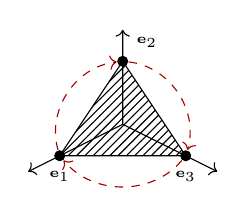
\begin{tikzpicture}[scale=0.8, baseline={(current bounding box.center)}]
        \tikzstyle{point}=[circle,fill,inner sep=0pt, minimum width=4pt, minimum height=4pt]

        % Triangle vertices
        \node[label=above right:\tiny$\bfe_2$] (e3)[point] at (1,1.5) {};
        \node[label=below:\tiny$\bfe_3$] (e1)[point] at (2,0) {};
        \node[label=below:\tiny$\bfe_1$] (e2)[point] at (0,0) {};

        % Barycenter
        \coordinate (bary) at (1,0.5) {}; 

        % Draw the triangle
        \draw[pattern=north east lines] (e1.center) -- (e2.center) -- (e3.center) -- cycle;

        % Compute extended axis endpoints
        \coordinate (e1_ext) at ($(bary) !1.5! (e1)$);
        \coordinate (e2_ext) at ($(bary) !1.5! (e2)$);
        \coordinate (e3_ext) at ($(bary) !1.5! (e3)$);

        % Draw coordinate axes
        \draw[->] (bary.center) -- (e1_ext);
        \draw[->] (bary.center) -- (e2_ext);
        \draw[->] (bary.center) -- (e3_ext);

        % Curved arrows showing clockwise direction around the triangle
        \draw[darkcandyapplered, dashed, ->, bend left=50] (e1) to (e2);
        \draw[darkcandyapplered, dashed, ->, bend left=50] (e2) to (e3);
        \draw[darkcandyapplered, dashed, ->, bend left=50] (e3) to (e1);
    \end{tikzpicture}
}

\newcommand{\triangleWithRotationn}{%
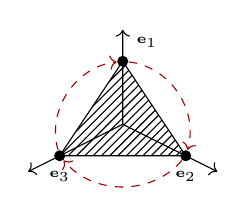
\begin{tikzpicture}[scale=0.8, baseline={(current bounding box.center)}]
        \tikzstyle{point}=[circle,fill,inner sep=0pt, minimum width=4pt, minimum height=4pt]

        % Triangle vertices
        \node[label=above right:\tiny$\bfe_1$] (e3)[point] at (1,1.5) {};
        \node[label=below:\tiny$\bfe_2$] (e1)[point] at (2,0) {};
        \node[label=below:\tiny$\bfe_3$] (e2)[point] at (0,0) {};

        % Barycenter
        \coordinate (bary) at (1,0.5) {}; 

        % Draw the triangle
        \draw[pattern=north east lines] (e1.center) -- (e2.center) -- (e3.center) -- cycle;

        % Compute extended axis endpoints
        \coordinate (e1_ext) at ($(bary) !1.5! (e1)$);
        \coordinate (e2_ext) at ($(bary) !1.5! (e2)$);
        \coordinate (e3_ext) at ($(bary) !1.5! (e3)$);

        % Draw coordinate axes
        \draw[->] (bary.center) -- (e1_ext);
        \draw[->] (bary.center) -- (e2_ext);
        \draw[->] (bary.center) -- (e3_ext);

        % Curved arrows showing clockwise direction around the triangle
        \draw[darkcandyapplered, dashed, ->, bend left=50] (e1) to (e2);
        \draw[darkcandyapplered, dashed, ->, bend left=50] (e2) to (e3);
        \draw[darkcandyapplered, dashed, ->, bend left=50] (e3) to (e1);
    \end{tikzpicture}
}

\newcommand{\triangleWithReflection}{%
    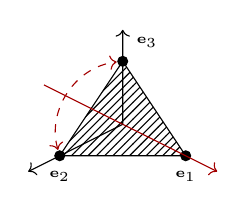
\begin{tikzpicture}[scale=0.8, baseline={(current bounding box.center)}]
        \tikzstyle{point}=[circle,fill,inner sep=0pt, minimum width=4pt, minimum height=4pt]

        % Triangle vertices
        \node[label=above right:\tiny$\bfe_3$] (e3)[point] at (1,1.5) {};
        \node[label=below:\tiny$\bfe_1$] (e1)[point] at (2,0) {};
        \node[label=below:\tiny$\bfe_2$] (e2)[point] at (0,0) {};

        % Barycenter
        \coordinate (bary) at (1,0.5) {}; 

        % Draw the triangle
        \draw[pattern=north east lines] (e1.center) -- (e2.center) -- (e3.center) -- cycle;

        % Compute extended axis endpoints
        \coordinate (e1_ext) at ($(bary) !1.5! (e1)$);
        \coordinate (e2_ext) at ($(bary) !1.5! (e2)$);
        \coordinate (e3_ext) at ($(bary) !1.5! (e3)$);

        % Draw coordinate axes
        \draw[darkcandyapplered,->] (bary.center) -- (e1_ext);
        \draw[->] (bary.center) -- (e2_ext);
        \draw[->] (bary.center) -- (e3_ext);

        % Make the e1 axis red and extend it beyond the midpoint of e2-e3
        \coordinate (mid_e2_e3) at ($(e2)!0.5!(e3)$); % Midpoint of e2 and e3
        \coordinate (e1_extended) at ($(e1)!1.5!(mid_e2_e3)$); % Extend e1 axis beyond midpoint
        \draw[darkcandyapplered] (bary.center) -- (e1_extended); % Red e1 axis extended
        
        \draw[darkcandyapplered, dashed, <->, bend left=50] (e2) to (e3);
    \end{tikzpicture}
}

\newcommand{\triangleWithReflectionn}{%
    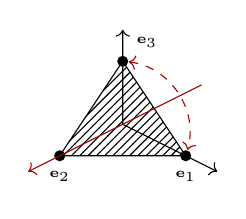
\begin{tikzpicture}[scale=0.8, baseline={(current bounding box.center)}]
        \tikzstyle{point}=[circle,fill,inner sep=0pt, minimum width=4pt, minimum height=4pt]

        % Triangle vertices
        \node[label=above right:\tiny$\bfe_3$] (e3)[point] at (1,1.5) {};
        \node[label=below:\tiny$\bfe_1$] (e1)[point] at (2,0) {};
        \node[label=below:\tiny$\bfe_2$] (e2)[point] at (0,0) {};

        % Barycenter
        \coordinate (bary) at (1,0.5) {}; 

        % Draw the triangle
        \draw[pattern=north east lines] (e1.center) -- (e2.center) -- (e3.center) -- cycle;

        % Compute extended axis endpoints
        \coordinate (e1_ext) at ($(bary) !1.5! (e1)$);
        \coordinate (e2_ext) at ($(bary) !1.5! (e2)$);
        \coordinate (e3_ext) at ($(bary) !1.5! (e3)$);

        % Draw coordinate axes
        \draw[->] (bary.center) -- (e1_ext);
        \draw[darkcandyapplered,->] (bary.center) -- (e2_ext);
        \draw[->] (bary.center) -- (e3_ext);

        % Make the e2 axis red and extend it beyond the midpoint of e1-e3
        \coordinate (mid_e1_e3) at ($(e1)!0.5!(e3)$); % Midpoint of e1 and e3
        \coordinate (e2_extended) at ($(e2)!1.5!(mid_e1_e3)$); % Extend e2 axis beyond midpoint
        \draw[darkcandyapplered] (bary.center) -- (e2_extended); % Red e2 axis extended

        % Curved clockwise arrows for the other axes
        \draw[darkcandyapplered, dashed, <->, bend left=50] (e3) to (e1);
    \end{tikzpicture}
}

\newcommand{\triangleWithReflectionnn}{%
    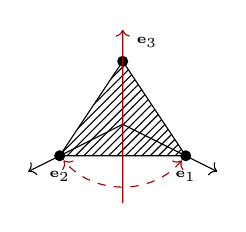
\begin{tikzpicture}[scale=0.8, baseline={(current bounding box.center)}]
        \tikzstyle{point}=[circle,fill,inner sep=0pt, minimum width=4pt, minimum height=4pt]

        % Triangle vertices
        \node[label=above right:\tiny$\bfe_3$] (e3)[point] at (1,1.5) {};
        \node[label=below:\tiny$\bfe_1$] (e1)[point] at (2,0) {};
        \node[label=below:\tiny$\bfe_2$] (e2)[point] at (0,0) {};

        % Barycenter
        \coordinate (bary) at (1,0.5) {}; 

        % Draw the triangle
        \draw[pattern=north east lines] (e1.center) -- (e2.center) -- (e3.center) -- cycle;

        % Compute extended axis endpoints
        \coordinate (e1_ext) at ($(bary) !1.5! (e1)$);
        \coordinate (e2_ext) at ($(bary) !1.5! (e2)$);
        \coordinate (e3_ext) at ($(bary) !1.5! (e3)$);

        % Draw coordinate axes
        \draw[->] (bary.center) -- (e1_ext);
        \draw[->] (bary.center) -- (e2_ext);
        \draw[darkcandyapplered,->] (bary.center) -- (e3_ext);

        % Make the e3 axis red and extend it beyond the midpoint of e1-e2
        \coordinate (mid_e1_e2) at ($(e1)!0.5!(e2)$); % Midpoint of e1 and e2
        \coordinate (e3_extended) at ($(e3)!1.5!(mid_e1_e2)$); % Extend e3 axis beyond midpoint
        \draw[darkcandyapplered] (bary.center) -- (e3_extended); % Red e3 axis extended

        % Curved clockwise arrows for the other axes
        \draw[darkcandyapplered, dashed, <->, bend left=50] (e1) to (e2);
    \end{tikzpicture}
}

% Start matrix with increased spacing
\matrix[column sep=2.5cm, row sep=.5cm] {
    % First row
    \node (T11) {\triangleWithAxes}; & \node (T12) {\triangleWithRotation}; & \node (T13) {\triangleWithRotationn}; \\
    % Second row
    \node (T21) {\triangleWithReflectionnn}; & \node (T22) {\triangleWithReflectionn}; & \node (T23) {\triangleWithReflection}; \\
};

% Add matrices with better spacing to avoid overlap
\node[left=0.2cm of T11] {$\begin{pmatrix} 1 & 0 & 0 \\ 0 & 1 & 0 \\ 0 & 0 & 1 \end{pmatrix}$};
\node[right=0.5cm of T11] {$\begin{pmatrix} 0 & 0 & 1 \\ 1 & 0 & 0 \\ 0 & 1 & 0 \end{pmatrix}$};
\node[right=0.5cm of T12] {$\begin{pmatrix} 0 & 1 & 0 \\ 0 & 0 & 1 \\ 1 & 0 & 0 \end{pmatrix}$};

\node[left=0.2cm of T21] {$\begin{pmatrix} 0 & 1 & 0 \\ 1 & 0 & 0 \\ 0 & 0 & 1 \end{pmatrix}$};
\node[right=0.5cm of T21] {$\begin{pmatrix} 0 & 0 & 1 \\ 0 & 1 & 0 \\ 1 & 0 & 0 \end{pmatrix}$};
\node[right=0.5cm of T22] {$\begin{pmatrix} 1 & 0 & 0 \\ 0 & 0 & 1 \\ 0 & 1 & 0 \end{pmatrix}$};

\node[above= 0.1cm of T11] {\text{Ταυτοτικός}};
\node[above= 0.1cm of T12] {\text{Στροφή κατά $120^\circ$}};
\node[above= 0.1cm of T13] {\text{Στροφή κατά $240^\circ$}};
\node[above= 0.001cm of T21] {\text{Ανάκλαση ως προς $x_3=0$}};
\node[above= 0.001cm of T22] {\text{$x_2=0$}};
\node[above= 0.001cm of T23] {\text{και $x_1=0$}};

\end{tikzpicture}
\]

Το σύνολο αυτών των έξι μετασχηματισμών αποτελεί ομάδα με πράξη τη σύνθεση (γιατί;), η οποία ονομάζεται \defn{ομάδα συμμετρίας} του $\Delta$. Οι ομάδες συμμετρίας τριγώνων μεγαλύτερης διάστασης θα είναι οι πρωταγωνιστές αυτών των σημειώσεων.

\begin{definition}
    \label{def:symmetricGroup}
    Έστω $S$ ένα σύνολο. \defn{Μετάθεση} του $S$ ονομάζεται κάθε αμφιμονοσήμαντη απεικόνιση $S \to S$. Το σύνολο $\fS(S)$ όλων των μεταθέσεων του $S$ με πράξη την σύνθεση απεικονίσεων αποτελεί ομάδα, η οποία ονομάζεται \defn{συμμετρική ομάδα} του $S$. Στην περίπτωση όπου $S = [n]$, τότε γράφουμε $\fS_n$.
\end{definition}

Μια μετάθεση $\pi \in \fS_n$ συνήθως γράφεται στην μορφή
\[
\begin{pmatrix}
    1     & 2     & \cdots & n \\
    \pi_1 & \pi_2 & \cdots & \pi_n
\end{pmatrix}
\]
όπου $\pi_i \coloneqq \pi(i)$, για κάθε $1 \le i \le n$, ή ως \emph{λέξη}
\[
\pi_1\pi_2\cdots\pi_n,
\]
ή στην \emph{κυκλική μορφή} ως γινόμενο ξένων κύκλων. Για παράδειγμα, 
\[
\pi \ = \ 
\begin{pmatrix}
    1 & 2 & 3 & 4 & 5 & 6 \\
    3 & 4 & 1 & 6 & 5 & 2
\end{pmatrix}
\ = \
341652
\ = \
\cycle{1,3}\cycle{2,4,6}\cycle{5} \ \in \fS_6.
\] 

Θα δούμε περισσότερα για τις μεταθέσεις και την συμμετρική ομάδα στην Παράγραφο \ref{sec:permutations}. Οι μεταθέσεις μπορούν να αναπαρασταθούν με πολλούς διαφορετικούς τρόπους, γεγονός που τις καθιστά ένα πολύ πλούσιο αντικείμενο μελέτης στην \emph{αλγεβρική συνδυαστική}. 

Ένα από τα στοιχεία που κάνουν τις ομάδες ενδιαφέρουσες είναι ότι δρουν σε διάφορα μαθηματικά αντικείμενα.

\begin{definition}
    \label{def:groupAction}
    Έστω $G$ μια ομάδα με ουδέτερο στοιχείο $\epsilon$ και $S$ ένα σύνολο. \defn{Δράση} της $G$ πάνω στο $S$ ονομάζεται μια απεικόνιση\footnote{Όπως και με την πράξη της ομάδας, έτσι και εδώ, συχνά θα παραλείπουμε το σύμβολο $\cdot$.} $\cdot : G \times S \to S$ τέτοια ώστε 
    %
    \begin{itemize}
        \item $g \cdot (h \cdot s) = (gh) \cdot s$
        \item $\epsilon \cdot s = s$
    \end{itemize}
    %
    για κάθε $g, h \in G$ και $s \in S$. Στην περίπτωση αυτή το $S$ ονομάζεται \defn{$G$-σύνολο}.
\end{definition}

Αν $S$ είναι ένα $G$-σύνολο, τότε η δράση κάθε στοιχείου $g \in G$ στο $S$ μεταθέτει τα στοιχεία του. Πιο συγκεκριμένα, η απεικόνιση 
\begin{align*}
    \sigma_g: S &\to S \\
    s &\mapsto gs
\end{align*}
είναι αμφιμονοσήμαντη (γιατί;).

Ένα $G$-σύνολο επάγει μια \emph{διαμέριση} της $S$ \emph{ταυτίζοντας} όλα εκείνα τα στοιχεία του $S$ τα οποία μπορούν να προκύψουν έπειτα από διαδοχικές εφαρμογές στοιχείων της $G$. Κάθε τέτοιο υποσύνολο του $S$
\[
\oO_s \coloneqq \{gs : g \in G\}
\] 
ονομάζεται \defn{τροχιά} (orbit) του $s$. Αν η ομάδα $G$ είναι πεπερασμένη, τότε 
%
\begin{equation}
    \label{eq:counting_formula}
    \abs{\oO_s} = \frac{\abs{G}}{\abs{G_s}},
\end{equation}
%
όπου $G_s$ είναι ο \defn{σταθεροποιητής} (stabilizer) του $s$ στην $G$, δηλαδή το σύνολο όλων των $g \in G$ τέτοια ώστε $gs = s$.

Για παράδειγμα, η συμμετρική ομάδα $\fS_n$ δρα στο $[n]$ με τον προφανή τρόπο:
\[
\pi \cdot i = \pi_i.
\]
Η δράση αυτή έχει ακριβώς \emph{μία} τροχιά και κατά συνέπεια $\abs{\oO_i} = n$, για κάθε $i \in [n]$. Τέτοιες δράσεις ονομάζονται \defn{μεταβατικές}. Η Ταυτότητα~\eqref{eq:counting_formula} μας πληροφορεί ότι 
\[
\abs{\left(\fS_n\right)_i} = (n-1)!,
\]
για κάθε $i \in [n]$. Πράγματι, ο σταθεροποιητής οποιουδήποτε στοιχείου του $[n]$ είναι ένα \textquote{αντίγραφο} της $\fS_{n-1}$ (γιατί;). 

Δεν είναι όμως όλες οι δράσεις μεταβατικές. Για παράδειγμα, για $n = 5$, θεωρούμε την υποομάδα της $\fS_5$ που παράγεται\footnote{Έστω $G$ μια ομάδα και $x_1, x_2, \dots, x_n$. Η υποομάδα της $G$ που παράγεται από τα $x_1, x_2, \dots, x_n$ περιέχει όλα τα στοιχεία της μορφής $x_{i_1}^{\pm1}x_{i_2}^{\pm1}\cdots x_{i_m}^{\pm1}$ για κάθε $1 \le i_1, i_2, \dots, i_m \le n$ και κάθε $m \ge 1$.} από τις αντιμεταθέσεις $\cycle{1,3}$ και $\cycle{2,5}$. Η δράση αυτή έχει τρεις τροχιές (γιατί;) και η επαγόμενη διαμέριση είναι 
\[
[5] \ = \ \{1, 3\} \uplus \{4\} \uplus \{2, 5\} .
\]

\begin{example}
    \label{ex:group_actions}
    Έστω $G$ μια ομάδα. Ας δούμε δύο σημαντικά παραδείγματα δράσεων ομάδων.
    \begin{itemize}
        \item[(1)] Έστω $H$ μια υποομάδα της $G$. Για $g \in G$, το σύνολο
        \[
        gH \coloneqq \{gh : h \in H\}
        \]
        ονομάζεται \defn{αριστερό σύμπλοκο} της $H$ στην $G$. 
        Το σύνολο των αριστερών συμπλόκων της $H$ επάγει μια διαμέριση της $G$
        \[
        G = t_1H \biguplus \, t_2H \biguplus \, \cdots \biguplus \, t_mH
        \]
        για κάποια\footnote{Το σύνολο $\{t_1, t_2, \dots, t_m\}$ συνήθως ονομάζεται \defn{σύστημα αντιπροσώπων} (system of representatives ή transversal) των αριστερών συμπλόκων της $H$.} $t_1, t_2, \dots, t_m \in G$, με φυσικό τρόπο, ταυτίζοντας δύο αριστερά σύμπλοκα $gH = xH$ αν και μόνο αν $x^{-1}g \in H$.

        Για παράδειγμα, αν $G = \fS_3$ και $H$ είναι η υποομάδα που παράγεται από την μετάθεση $\cycle{2,3}$, τότε έχουμε τη διαμέριση 
        \[
        \fS_3 = H \uplus \cycle{1,2}H \uplus \cycle{1,3}H.
        \]
        Παρατηρούμε ότι $\cycle{1,2}H = \cycle{1,2,3}H$ αφού 
        \[
        \cycle{1,2,3}^{-1}\cycle{1,2} = \cycle{1,3,2}\cycle{1,2} = \cycle{2,3} \ \in H.
        \]
        Ομοίως για το $\cycle{1,3}H = \cycle{1,3,2}H$.

        H $G$ δρα μεταβατικά στο σύνολο των αριστερών συμπλόκων της $H$, θέτοντας
        \[
        x \cdot gH = (xg)H,
        \]
        για κάθε $x ,g \in G$. Στην περίπτωση όπου $H = \{\epsilon\}$ είναι η τετριμμένη υποομάδα, τότε η $G$ δρα στον εαυτό  με \defn{αριστερό πολλαπλασιασμό}, δηλαδή 
        \[
        x \cdot g = xg. 
        \]

        \item[(2)] Η $G$ δρα στον εαυτό της με \defn{συζυγία}, θέτοντας
        \[
        g \cdot x = gxg^{-1}
        \]
        για κάθε $x, g \in G$. Οι τροχιές αυτής της δράσης ονομάζονται \defn{κλάσεις συζυγίας}. Δύο στοιχεία $t, x \in G$ που ανήκουν στην ίδια τροχιά, δηλαδή αν $x = gtg^{-1}$, για κάποιο $g \in G$ ονομάζονται \defn{συζυγή}. 

        Αν η $G$ είναι πεπερασμένη, το πλήθος των στοιχείων μιας κλάσης συζυγίας μπορεί να υπολογιστεί από την Ταυτότητα~\eqref{eq:counting_formula}. Το να έχει μια κλάση συζυγίας ένα μόνο στοιχείο $x$ σημαίνει ότι $x = gxg^{-1}$, \emph{για κάθε} $g \in G$. Το σύνολο όλων των στοιχείων της $G$ με αυτή την ιδιότητα ονομάζεται \defn{κέντρο} της $G$ και συμβολίζεται με $\rmZ(G)$.

        Για παράδειγμα, η συμμετρική ομάδα $\fS_3$ έχει τρεις κλάσεις συζυγίας: 
        \[
        \fS_3 = \{\cycle{1,2,3}\} \uplus \{\cycle{1,2}, \cycle{2,3}, \cycle{1,3}\} \uplus \{\cycle{1,2,3}, \cycle{1,3,2}\}.
        \]
    \end{itemize}
\end{example}

Στην περίπτωση όπου έχουμε ένα $G$-σύνολο $S$, μπορούμε να \textquote{αναπαραστήσουμε} την $G$ ως υποομάδα της ομάδας συμμετρίας του $S$. Πιο συγκεκριμένα, η απεικόνιση 
\begin{align*}
    \sigma : G &\to \fS(S) \\
    g &\mapsto \sigma_g
\end{align*}
είναι \emph{ομομορφισμός ομάδων}, δηλαδή ικανοποιεί τις σχέσεις:
\begin{align*}
    \sigma(\epsilon) &= \rmid_S \\ 
    \sigma(gx) &= \sigma_g\sigma_x
\end{align*}
για κάθε $g, x \in G$ (γιατί;).

Πίσω στο παράδειγμα του τριγώνου $\Delta$, η συμμετρική ομάδα $\fS_3$ δρα στον $\RR^3$, και κατά συνέπεια στο $\Delta$, μεταθέτοντας τα στοιχεία της βάσης του (δηλαδή, τις κορυφές του $\Delta$):
\[
w\cdot \bfe_i = \bfe_{w_i},
\] 
για κάθε $w\in \fS_3$ και $1 \le i \le 3$. Κάθε $w \in \fS_3$ επάγει μια διαφορετική μετάθεση $\sigma(w)$ (γιατί;). Οι δράσεις με αυτή την ιδιότητα ονομάζονται \defn{πιστές}. Συνεπώς, η $\sigma$ είναι \textquote{πιστή αναπαράσταση} της $\fS_3$ ως ομάδα συμμετρίας του $\Delta$.

Στην περίπτωση αυτή, το σύνολο $\RR^3$ έχει την έξτρα δομή του \emph{διανυσματικού χώρου} και κάθε μετάθεση $\sigma(w)$ είναι \emph{γραμμικός μετασχηματισμός}. Υπολογίζοντας του πίνακες ως προς τη συνήθη βάση $\{\bfe_1, \bfe_2, \bfe_3\}$ βρίσκουμε 
\begin{alignat*}{3}
    \sigma(\cycle{1}\cycle{2}\cycle{3}) &= 
    \begin{pmatrix} 
        1 & 0 & 0 \\ 
        0 & 1 & 0 \\ 
        0 & 0 & 1 
    \end{pmatrix}  
    &\quad \sigma(\cycle{1,2,3}) &= 
    \begin{pmatrix} 
        0 & 0 & 1 \\ 
        1 & 0 & 0 \\ 
        0 & 1 & 0 
    \end{pmatrix}
    &\quad \sigma(\cycle{1,3,2}) &= 
    \begin{pmatrix} 
        0 & 1 & 0 \\ 
        0 & 0 & 1 \\ 
        1 & 0 & 0 
    \end{pmatrix} \\[15pt]
    \sigma(\cycle{1,2}) &=
    \begin{pmatrix} 
        0 & 1 & 0 \\ 
        1 & 0 & 0 \\ 
        0 & 0 & 1 
    \end{pmatrix} 
    &\quad \sigma(\cycle{1,3}) &= 
    \begin{pmatrix} 
        0 & 0 & 1 \\ 
        0 & 1 & 0 \\ 
        1 & 0 & 0 
    \end{pmatrix} 
    &\quad \sigma(\cycle{2,3}) &= 
    \begin{pmatrix} 
        0 & 0 & 1 \\ 
        1 & 0 & 0 \\ 
        0 & 1 & 0 
    \end{pmatrix} 
\end{alignat*}
Οι μετασχηματισμοί αυτοί είναι οι συμμετρίες του $\Delta$ που συναντήσαμε νωρίτερα! Αυτή είναι και η βασική ιδέα της αναπαράστασης μιας ομάδας.

\begin{definition}
    \label{def:representation}
    Έστω $G$ μια ομάδα. \defn{Αναπαράσταση} (representation) της $G$ ονομάζεται ένα ζεύγος $(\rho, V)$, όπου 
    \begin{itemize}
    \item $V$ είναι διανυσματικός χώρος 
    \item $\rho : G \to \GL(V)$ είναι ένας ομομορφισμός ομάδων, 
    \end{itemize}
    όπου με $\GL(V)$ συμβολίζουμε την ομάδα των αντιστρέψιμων γραμμικών μετασχηματισμών του $V$\footnote{H $\GL(V)$ ονομάζεται \defn{γενική γραμμική} ομάδα του $V$.}. Η διάσταση του $V$ ονομάζεται \defn{διάσταση} (ή \defn{βαθμός}) της αναπαράστασης.
\end{definition}

Με άλλα λόγια, αναπαράσταση της $G$ είναι ένα $G$-σύνολο $V$ με δομή διανυσματικού χώρου, την οποία \textquote{σέβεται} η δράση. Συχνά, αντί για $\rho(g)(v)$ θα γράφουμε απλώς $g \cdot v$, ή ακόμα πιο απλά $gv$. Στην περίπτωση αυτή θα λέμε ότι το $V$ είναι ένα \defn{$G$-πρότυπο}. Επίσης, αν ο $V$ έχει πεπερασμένη διάσταση, τότε διαλέγοντας μια βάση του $V$ μπορούμε να αναπαραστήσουμε το $\rho(g)$ με έναν αντιστρέψιμο πίνακα. Σε ότι ακολουθεί, θα εναλλάσσουμε μεταξύ πινάκων και γραμμικών μετασχηματισμών χωρίς να το αναφέρουμε, αλλά θα είναι κατανοητό από τα συμφραζόμενα.

Τι γίνεται όμως αν έχουμε μια δράση σ' ένα σύνολο που δεν έχει (απαραίτητα) τη δομή διανυσματικού χώρου; Κάθε δράση ομάδας επάγει μια αναπαράσταση ως εξής. Έστω $S = \{s_1, s_2, \dots, s_n\}$ ένα $G$-σύνολο και $\FF[S]$ ο διανυσματικός χώρος που παράγεται από το $S$\footnote{Στην πράξη θα γράφουμε $\FF[s_1, s_2, \dots, s_n]$ \textquote{ξεχνώντας} τις αγκύλες και θα αναφερόμαστε στο $S$ ως  τη \defn{συνήθη βάση} του χώρου αυτού.}. Επεκτείνουμε γραμμικά την δράση στο $\FF[S]$ θέτοντας 
\[
g\left(c_1s_1 + c_2s_2 + \cdots + c_ns_n\right) \ =
c_1 gs_1 + c_2 gs_2 + \cdots + c_n gs_n
\] 
για κάθε $g \in G$ και $c_1, c_2, \dots, c_n \in \FF$, δίνοντας έτσι στο $\FF[S]$ την δομή $G$-προτύπου.

Η αντίστοιχη αναπαράσταση ονομάζεται \defn{αναπαράσταση μεταθέσεων} (permutation representation). Τέτοιου είδους αναπαραστάσεις είναι πολύ σημαντικές, διότι μας επιτρέπουν να χρησιμοποιούμε μεθόδους συνδυαστικής για να μελετήσουμε την ομάδα.

Ας δούμε μερικά σημαντικά παραδείγματα αναπαραστάσεων.
\begin{example}
    \label{ex:representations_examples}
    Έστω $G$ μια ομάδα και $H$ υποομάδα της.
    \leavevmode
    \begin{itemize}
        \item[(α)] Κάθε διανυσματικός χώρος $V$ διάστασης 1 γίνεται $G$-πρότυπο θέτοντας 
        \[
        gv = v
        \]
        για κάθε $g \in G$ και $v \in V$. Η αντίστοιχη αναπαράσταση ονομάζεται \defn{τετριμμένη αναπαράσταση} (trivial representation) της $G$ και την συμβολίζουμε με $(\rho^\triv, V)$. Όταν αναφερόμαστε στο αντίστοιχο πρότυπο γράφουμε $V^\triv$.
        \item[(β)] Η αναπαράσταση μεταθέσεων που επάγεται από την δράση της $G$ στον εαυτό της με αριστερό πολλαπλασιασμό ονομάζεται \defn{κανονική αναπαράσταση} (regular representation) της $G$ και την συμβολίζουμε με $(\rho^\reg, \FF[G])$. Όπως θα δούμε στην Παράγραφο \ref{sec:regular_representation}, η κανονική αναπαράσταση αποτελεί ένα από τα σημαντικότερα παραδείγματα αναπαραστάσεων.
        \item[(γ)] Η αναπαράσταση μεταθέσεων που επάγεται από τη δράση της $G$ στο σύνολο των αριστερών συμπλόκων της $H$ ονομάζεται \defn{αναπαράσταση συμπλόκου} (coset representation). Στην περίπτωση όπου $H = \{\epsilon\}$ είναι η τετριμμένη υποομάδα, τότε η αναπαράσταση συμπλόκου εξειδικεύεται στην κανονική αναπαράσταση. Όπως θα δούμε στην Παράγραφο \ref{sec:frobenius_reciprocity}, η αναπαράσταση συμπλόκου είναι ειδική περίπτωση μιας \emph{επαγόμενης αναπαράστασης} (induced representation) μεγάλου ενδιαφέροντος.
    \end{itemize}
    %
    Για τα υπόλοιπα παραδείγματα υποθέτουμε ότι $G = \fS_n$.
    %
    \begin{itemize}
        \item[(δ)] Ο πίνακας της μετάθεσης $\cycle{1,2}$ στην κανονική αναπαράσταση της $\fS_3$ ως προς τη συνήθη βάση $\{\cycle{1}\cycle{2}\cycle{3}, 
        \cycle{1,2}, 
        \cycle{2,3}, 
        \cycle{1,3}, 
        \cycle{1,2,3}, 
        \cycle{1,3,2}\}$ του $\FF[\fS_3]$ είναι   
        \[
        \begin{pmatrix}
            0 & 1 & 0 & 0 & 0 & 0 \\
            1 & 0 & 0 & 0 & 0 & 0 \\
            0 & 0 & 0 & 0 & 1 & 0 \\
            0 & 0 & 0 & 0 & 0 & 1 \\
            0 & 0 & 1 & 0 & 0 & 0 \\
            0 & 0 & 0 & 1 & 0 & 0
        \end{pmatrix}.
        \]
        Γιατί; Ποιοί είναι οι υπόλοιποι; Τι παρατηρείτε;
        \item[(στ)] Έστω $H$ η υποομάδα της $\fS_3$ που παράγεται από την μετάθεση $\cycle{2,3}$. Ο πίνακας της μετάθεσης $\cycle{1,2}$ στην αντίστοιχη αναπαράσταση συμπλόκου ως προς τη συνήθη βάση $\{H, \cycle{1,2}H, \cycle{1,3}H\}$ είναι 
        \[
        \begin{pmatrix}
            0 & 1 & 0 \\
            1 & 0 & 0 \\
            0 & 0 & 1
        \end{pmatrix}.
        \]
        Γιατί; Ποιοί είναι οι υπόλοιποι; Τι παρατηρείτε;
        \item[(ζ)] Εκτός από την τετριμμένη αναπαράσταση, η συμμετρική ομάδα έχει μια ακόμη αναπαράσταση διάστασης 1, η οποία προκύπτει με φυσικό τρόπο. Ένας διανυσματικός χώρος $V$ διάστασης 1 γίνεται $\fS_n$-πρότυπο θέτοντας
        \[
        \pi v = \sign(\pi)v,
        \]
        για κάθε $\pi \in \fS_n$ και $v \in V$, όπου $\sign(\pi)$ είναι το \defn{πρόσημο} της μετάθεσης $\pi$ (βλ. Ορισμός \ref{def:sign_permutation}). Η αναπαράσταση αυτή ονομάζεται \defn{αναπαράσταση προσήμου} (sign representation) και την συμβολίζουμε με $(\rho^\sign,V)$. Όταν αναφερόμαστε στο αντίστοιχο πρότυπο γράφουμε $V^\sign$.
        \item[(η)] Η αναπαράσταση μεταθέσεων που επάγεται από την προφανή δράση της $\fS_n$ στο $[n]$ ονομάζεται \defn{αναπαράσταση καθορισμού} (defining representation) και την συμβολίζουμε με $\left(\rho^\rmdef,\FF[1,2,\dots,n]\right)$. Όταν αναφερόμαστε στο αντίστοιχο πρότυπο γράφουμε $V^\rmdef$. Για $\pi \in \fS_n$, ως προς τη συνήθη βάση έχουμε   
        \[
       \left(\rho^\rmdef(\pi)\right)_{ij} = 
        \begin{cases}
            1, &\ \text{αν $\pi_j = i$} \\
            0, &\ \text{διαφορετικά}
        \end{cases}
        \]
        για κάθε $1 \le i, j \le n$ (γιατί;). Πίνακες αυτής της μορφής ονομάζονται \defn{πίνακες μετάθεσης} (permutation matrices). Ποιοί είναι οι πίνακες μετάθεσης για $n=3$; Τι παρατηρείτε;
    \end{itemize}
\end{example}

Επιστρέφοντας στο τρέχον παράδειγμα με την αναπαράσταση της $\fS_3$ ως ομάδα συμμετρίας του $\Delta$, ας \textquote{αλλάξουμε οπτική}, γράφοντας τους πίνακες $\sigma(w)$ στην βάση 
\[
\{\bfe_1 + \bfe_2 + \bfe_3, \bfe_2-\bfe_1, \bfe_3-\bfe_1\}
\]
του $\RR^3$:
\begin{alignat*}{3}
    \sigma(\cycle{1}\cycle{2}\cycle{3}) &= 
    \begin{pmatrix} 
        1 & 0 & 0 \\ 
        0 & 1 & 0 \\ 
        0 & 0 & 1 
    \end{pmatrix}    
    &\ \sigma(\cycle{1,2,3}) &= 
    \begin{pmatrix} 
        1 & 0 & 0 \\ 
        0 & -1 & -1 \\ 
        0 & 1 & 0 
    \end{pmatrix}
    &\ \sigma(\cycle{1,3,2}) &= 
    \begin{pmatrix} 
        1 & 0 & 0 \\ 
        0 & 0 & 1 \\ 
        0 & -1 & -1 
    \end{pmatrix} \\[15pt]
    \sigma(\cycle{1,2}) &=
    \begin{pmatrix} 
        1 & 0 & 0 \\ 
        0 & -1 & -1 \\ 
        0 & 0 & 1 
    \end{pmatrix}
    &\ \sigma(\cycle{1,3}) &= 
    \begin{pmatrix} 
        1 & 0 & 0 \\ 
        0 & 1 & 0 \\ 
        0 & -1 & -1 
    \end{pmatrix} 
    &\ \sigma(\cycle{2,3}) &= 
    \begin{pmatrix} 
        1 & 0 & 0 \\ 
        0 & 0 & 1 \\ 
        0 & 1 & 0 
    \end{pmatrix}.
\end{alignat*}

Συνεπώς, έχουμε μια διάσπαση
%
\begin{equation}
\label{eq:decomposition_R3}
\RR^3 = \RR[\bfe_1+\bfe_2+\bfe_3] \oplus \RR[\bfe_2-\bfe_1, \bfe_3-\bfe_1],
\end{equation}
%
η οποία \textquote{σέβεται} τη δράση της συμμετρικής ομάδας. 
Επιπλέον, παρατηρούμε ότι η $\fS_3$ δρα στον υπόχωρο $\RR[\bfe_1+\bfe_2+\bfe_3]$ τετριμμένα.

\begin{definition}
    \label{def:subrepresentation}
    Έστω $(\rho, V)$ αναπαράσταση μιας ομάδας $G$ και $W$ ένας υπόχωρος του $V$. Το ζεύγος $(\rho,W)$ ονομάζεται \defn{υποαναπαράσταση} (ή \defn{$G$-υποπρότυπο}, στην γλώσσα των προτύπων) της $V$ αν ο $W$ είναι \emph{$G$-αναλλοίωτος}, δηλαδή αν για κάθε $g \in G$ ισχύει ότι 
    \[
    \rho(g)(w) \in W
    \]
    για κάθε $w \in W$.
\end{definition}

Στην αναπαράσταση καθορισμού (όπως και στην περίπτωση της αναπαράστασης του τρέχοντος παραδείγματος) ο υπόχωρος 
\[
W = \FF[1 + 2 + \cdots + n] = \{c(1+2+ \cdots + n) : c \in \FF\}
\]
είναι $\fS_n$-αναλλοίωτος, διότι
\[
\pi \cdot (1+2+\cdots+n) = \pi_1 + \pi_2 + \cdots + \pi_n = 1 + 2 + \cdots + n \ \in \ W,
\]
για κάθε $\pi \in \fS_n$. Συνεπώς, βρήκαμε μια υποαναπαράσταση της $\FF[1,2,\dots,n]$ διάστασης ένα, η οποία είναι \textquote{αντίγραφο} της τετριμμένης αναπαράστασης. Γενικότερα, κάθε αναπαράσταση μεταθέσεων σ' ένα σύνολο $S = \{s_1, s_2, \dots, s_n\}$ περιέχει την μονοδιάστατη υποαναπαράσταση $\FF[s_1 + s_2 + \cdots + s_n]$ (γιατί;).

\begin{definition}
    \label{def:irreducible_representation}
    Μια αναπαράσταση η οποία περιέχει μια γνήσια υποαναπαράσταση, που δεν είναι ο τετριμμένος υπόχωρος, ονομάζεται \defn{αναγωγική} (reducible). Διαφορετικά, την αποκαλούμε \defn{ανάγωγη} (irreducible) αναπαράσταση.
\end{definition}

Κάθε μονοδιάσταση αναπαράσταση είναι κατ' ανάγκη ανάγωγη (γιατί;) και κάθε αναπαράσταση μεταθέσεων είναι αναγωγική (γιατί;).

\begin{proposition}
    \label{prop:irreducible_representation_criterion}
    Έστω $G$ μια ομάδα. Μια αναπαράσταση $(\rho,V)$ πεπερασμένης διάστασης της $G$ είναι αναγωγική αν και μόνο αν υπάρχει μια βάση του $V$ τέτοια ώστε ο πίνακας της $\rho(g)$ ως προς αυτή την βάση να είναι μπλόκ-άνω τριγωνικός, για κάθε $g \in G$.
\end{proposition}

\begin{proof}[Απόδειξη]
Έστω $\dim(V) = n$. Για την κατεύθυνση \textquote{$\then$}, υποθέτουμε ότι $W$ είναι υποαναπαράσταση του $V$ με βάση $\{w_1, w_2, \dots, w_k\}$. Συμπληρώνουμε την βάση αυτή με στοιχεία του $V$, για να πάρουμε μια βάση $\{w_1, w_2, \dots, w_k, v_{k+1}, \dots, v_n\}$ του $V$. Για κάθε $g \in G$, ο πίνακας $\rho(g)$ ως προς αυτή την βάση έχει την ζητούμενη μορφή, διότι 
\[
\rho(g)(w_i) \ \in W
\]
για κάθε $1 \le i \le k$.

Αντιστρόφως, υποθέτουμε ότι υπάρχει μια βάση του $V$ ως προς την οποία, για κάθε $g \in G$
\[
\rho(g) = 
\begin{pmatrix}
    A & \ast \\ 
    0 & B
\end{pmatrix}
\]
όπου $A, B$ είναι τετραγωνικοί πίνακες. Αν ο $A$ είναι $k\times{k}$, τότε ο υπόχωρος που παράγεται από τα πρώτα $k$ στοιχεία της βάσης αυτής είναι $G$-αναλλοίωτος (γιατί;) και το ζητούμενο έπεται.
\end{proof}

Στο τρέχον παράδειγμα, είδαμε ότι ο υπόχωρος $\RR[\bfe_1+\bfe_2+\bfe_3]$ είναι υποαναπαράσταση. Μιμούμενοι την απόδειξη της Πρότασης~\ref{prop:irreducible_representation_criterion}, μπορούμε να επεκτείνουμε τη βάση με τον προφανή τρόπο
\[
\{\bfe_1+\bfe_2+\bfe_3, \bfe_2, \bfe_3\}
\]
και υπολογίζοντας τους πίνακες των $\sigma(w)$ ως προς αυτή τη βάση βρίσκουμε 
\begin{alignat*}{3}
    \sigma(\cycle{1}\cycle{2}\cycle{3}) &= 
    \begin{pmatrix} 
        1 & 0 & 0 \\ 
        0 & 1 & 0 \\ 
        0 & 0 & 1 
    \end{pmatrix}    
    &\ \sigma(\cycle{1,2,3}) &= 
    \begin{pmatrix} 
        1 & 0 & 1 \\ 
        0 & 0 & -1 \\ 
        0 & 1 & -1 
    \end{pmatrix}
    &\ \sigma(\cycle{1,3,2}) &= 
    \begin{pmatrix} 
        1 & 1  & 0 \\ 
        0 & -1 & 1 \\ 
        0 & -1 & 0
    \end{pmatrix} \\[15pt]
    \sigma(\cycle{1,2}) &=
    \begin{pmatrix} 
        1 & 1  & 0 \\ 
        0 & -1 & 0 \\ 
        0 & 0  & 1 
    \end{pmatrix} 
    &\ \sigma(\cycle{1,3}) &= 
    \begin{pmatrix} 
        1 & 0 & 0 \\ 
        0 & 1 & 1 \\ 
        0 & 0 & 0
    \end{pmatrix} 
    &\ \sigma(\cycle{2,3}) &= 
    \begin{pmatrix} 
        1 & 0 & 1 \\ 
        0 & 0 & -1 \\ 
        0 & 1 & -1 
    \end{pmatrix},
\end{alignat*}
όπως προέβλεψε η Πρόταση~\ref{prop:irreducible_representation_criterion}. Αλλά, ο υπόχωρος $\RR[\bfe_2,\bfe_3]$ \emph{δεν} είναι $\fS_3$-αναλλοίωτος, διότι 
\[
\cycle{1,2} \cdot \bfe_2 = \bfe_1 \ \notin \ \RR[\bfe_2, \bfe_3]
\]
και κατ' επέκταση δεν αποτελεί υποαναπαράσταση. Συνεπώς, η διάσπαση 
\[
\RR^3 = \RR[\bfe_1+\bfe_2+\bfe_3] \oplus \RR[\bfe_2,\bfe_3]
\]
δεν \textquote{σέβεται} της δράση της συμμετρικής ομάδας, σ' αντίθεση με αυτή της Διάσπασης~\eqref{eq:decomposition_R3}, γεγονός το οποίο εξηγεί γιατί οι αντίστοιχοι πίνακες της τελευταίας περίπτωσης είναι μπλοκ-διαγώνιοι.

\section{Πλήρης αναγωγικότητα και το Θεώρημα του Maschke}
\label{sec:maschke}

Σε αυτή την παράγραφο υποθέτουμε ότι το σώμα $\FF$ είναι είτε το $\RR$, είτε το $\CC$ και θεωρούμε μια πεπερασμένη ομάδα $G$.

Συνεχίζοντας το τρέχον παράδειγμα της προηγούμενης παραγράφου, παρατηρούμε ότι ο υπόχωρος $\RR[\bfe_2-\bfe_1,\bfe_3-\bfe_1]$ αποτελείται από όλα εκείνα τα στοιχεία του $\RR^3$ που είναι \emph{ορθογώνια} με το $\bfe_1 + \bfe_2 + \bfe_3$ ως προς το σύνηθες εσωτερικό γινόμενο, δηλαδή
\[
\RR[\bfe_2-\bfe_1,\bfe_3-\bfe_1] =
\{(v_1, v_2, v_3) \in \RR^3 : v_1 + v_2 + v_3 = 0\},
\] 
τ' οποίο επιπλέον \textquote{σέβεται} τη δράση της $\fS_3$. Ας θυμηθούμε τον ορισμό του εσωτερικού γινομένου.

\begin{definition}
    \label{def:inner_product}
    Έστω $V$ διανυσματικός χώρος. \defn{Εσωτερικό γινόμενο} στον $V$ ονομάζεται μια απεικόνιση $(\Arg,\Arg) : V\times V \to \FF$ η οποία είναι
    %
    \begin{itemize}
        \item \emph{γραμμική} ως προς την πρώτη μεταβλητή, δηλαδή
        \[
            (v+cv', u) = (v,u) + c(v',u),
        \]
        για κάθε $v, v', u \in V$ και $c \in \FF$,
        \item \emph{συζυγής-συμμετρική}, δηλαδή 
        \[
        (v,u) = \ol{(u,v)},
        \]
        για κάθε $u, v \in V$, και 
        \item \emph{θετικά ορισμένη}, δηλαδή  
        \[
        (v,v) > 0, \quad \text{αν $v \neq 0$}.
        \]
    \end{itemize}
    %
    Επιπλέον, αν $W$ είναι υπόχωρος του $V$, τότε το σύνολο 
    \[
    W^\perp \coloneqq \{v \in V : (v,w) = 0, \ \text{για κάθε $w \in W$}\}
    \]
    ονομάζεται \defn{ορθογώνιο συμπλήρωμα} του $W$ στο $V$ ως προς το $(\Arg, \Arg)$.
\end{definition}

Το επόμενο αποτέλεσμα εξηγεί γιατί επιλέξαμε τον υπόχωρο $\RR[\bfe_2-\bfe_1,\bfe_3-\bfe_1]$ στο τρέχον παράδειγμα, έναντι κάποιου άλλου όπως, για παράδειγμα, τον $\RR[\bfe_2,\bfe_3]$.

\begin{proposition}
    \label{prop:invariant_inner_product}
    Έστω $V$ ένα $G$-πρότυπο και $W$ υποπρότυπο του $V$. Αν $(\Arg,\Arg)$ είναι ένα \emph{$G$-αναλλοίωτο} εσωτερικό γινόμενο στον $V$, δηλαδή 
    \[
    (gv, gu) = (v,u),
    \]
    για κάθε $g \in G$ και $v, u \in V$, τότε το ορθογώνιο συμπλήρωμα του $W$ στο $V$ ως προς αυτό είναι υποπρότυπο του $V$.
\end{proposition}

\begin{proof}[Απόδειξη]
    Αρκεί να δείξουμε ότι $gu \in W^\perp$, δηλαδή ότι $(gu, w) = 0$, για κάθε $g \in G$, $u \in W^\perp$ και $w \in W$. Πράγματι, 
    \[
    (gu, w) = (g^{-1}gu, g^{-1}w) = (u, g^{-1}w) = 0,
    \]
    όπου η πρώτη ισότητα έπεται από το ότι το $(\Arg,\Arg)$ είναι $G$-αναλλοίωτο και η τρίτη από το ότι το $W$ είναι υποπρότυπο του $V$. 
\end{proof}

Το να έχει μια αναπαράσταση $(\rho, V)$ ένα $G$-αναλλοίωτο εσωτερικό γινόμενο σημαίνει ότι για κάθε $g \in G$ ο μετασχηματισμός $\rho(g)$ είναι \emph{μοναδιαίος} (unitary), δηλαδή\footnote{Ο πίνακας $A^\ast \coloneqq \ol{A}^\top$ ονομάζεται \defn{προσηρτημένος} (adjoint) του $A$. Από την γραμμική άλγεβρα γνωρίζουμε ότι στην περίπτωση που έχουμε έναν μοναδιαίο πίνακα $A$ με στοιχεία στο $\CC$    , τότε υπάρχει μια \emph{ορθοκανοκική βάση} του $V$, η οποία αποτελείται από \emph{ιδιοδιανύσματα} του $A$ μήκους 1.}  
\[
\rho(g)^{-1} =  \ol{\rho(g)}^\top,
\]
όπου με $\ol{A}$ συμβολίζουμε τον πίνακα που προκύπτει από τον $A$ παίρνοντας τα συζηγή όλων των στοιχείων του και με $A^\top$ συμβολίζουμε τον ανάστροφο του $A$. Με άλλα λόγια, ο $\rho(g)$ πρέπει να είναι \emph{ισομετρία}. Στην περίπτωση όπου $\FF = \RR$, οι μοναδιαίοι πίνακες ονομάζονται \emph{ορθογώνιοι}. Παραδείγματα ορθογώνιων πινάκων αποτελούν οι πίνακες των μετασχηματισμών της στροφής και της ανάκλασης.

Ας δούμε ένα παράδειγμα μη-αναλλοίωτου εσωτερικού γινομένου. Έστω $\rmC_2$ η κυκλική ομάδα τάξης 2, η οποία παράγεται από ένα στοχείο $g$, δηλαδή $\rmC_2 = \{\epsilon, g\}$. Θεωρούμε τη δράση της $\rmC_2$ στον $\RR^2$ που ορίζεται ως εξής
\[
\begin{tikzpicture}[>=stealth, thick, scale=1]
    \begin{scope}[shift={(-1,0)}]
        % Axes
        \draw[->] (-1.5,0) -- (1.5,0);
        \draw[->] (0,-1.5) -- (0,1.5);

        % Vectors e1 and e2
        \draw[->, burntorange, very thick] (0,0) -- (1,0) node[below] {\textcolor{black}{$\bfe_1$}};
        \draw[->, iceberg, very thick] (0,0) -- (0,1) node[left] {\textcolor{black}{$\bfe_2$}};

        % Origin dot
        \fill (0,0) circle (1.5pt);
    \end{scope}
    \begin{scope}[shift={(6,0)}]
        % Axes
        \draw[->,burntorange!40] (-1.5,0) -- (1.5,0);
        \draw[->] (0,-1.5) -- (0,1.5);

        % Vectors
        \draw[->, burntorange, very thick] (0,0) -- (1,0) node[above] {\textcolor{black}{$\bfe_1$}};
        \draw[->, iceberg, very thick] (0,0) -- (1,-1) node[below] {\textcolor{black}{$\bfe_1 - \bfe_2$}};

        % Origin dot
        \fill (0,0) circle (1.5pt);
    \end{scope}

  % --- Curved arrow between them ---
    \draw[->, thick]
    (1.7,0.3) .. controls (2,0.7) and (3,0.7) .. (3.3,0.3)
    node[midway, above] {$g$};
\end{tikzpicture}
\]
Ισοδύναμα, έχουμε την αναπαράσταση $\rho : \rmC_2 \to \GL(\RR^2)$ με 
\[
\rho(\epsilon) = 
\begin{pmatrix}
    1 & 0 \\
    0 & 1
\end{pmatrix}
\quad
\text{και}
\quad
\rho(g) = 
\begin{pmatrix}
    1 & 1 \\
    0 & -1
\end{pmatrix}.
\]
Ο υπόχωρος $\RR[\bfe_1]$ διάστασης 1 που παράγεται από το $\bfe_1$ είναι $\rmC_2$-αναλλοίωτος (γιατί;). Ας \textquote{κοιτάξουμε} το ορθογώνιο συμπλήρωμά του ως προς το σύνηθες εσωτερικό γινόμενο 
\[
\RR[\bfe_1]^\perp  = \{v \in \RR^2 : v\cdot\bfe_1 = 0\} = \{v = (v_1, v_2) \in \RR^2 : v_1= 0\} = \RR[\bfe_2].
\]
Τότε, 
\[
g\bfe_2 = \bfe_1 - \bfe_2 \ \notin \RR[\bfe_2]
\]
και κατά συνέπεια το ορθογώνιο συμπλήρωμα του $\RR[\bfe_1]$ δεν είναι $\rmC_2$-αναλλοίωτο. Αυτό συμβαίνει διότι το σύνηθες εσωτερικό γινόμενο \emph{δεν} είναι $\rmC_2$-αναλλοίωτο!

Αποδεικνύεται όμως ότι κάθε αναπαράσταση πεπερασμένης διάστασης επιδέχεται ένα $G$-αναλ\-λοίωτο εσωτερικό γινόμενο. Πως θα μπορούσαμε να \textquote{τροποποιήσουμε} το σύνηθες εσωτερικό γινόμενο ώστε να \textquote{σέβεται} τη δράση της $\rmC_2$ στο παράδειγμα της προηγούμενης παραγράφου; Ας δούμε \textquote{πόσο έξω πέφτει} στην δράση του $g$ στην συνήθη βάση: 
\[
g\bfe_1 \cdot g\bfe_2 = \bfe_1 \cdot(\bfe_1-\bfe_2) = \bfe_1\cdot\bfe_1 - \bfe_1\cdot\bfe_2 = 1 - 0 = 1.
\]
Κατά έναν παράγοντα $\bfe_1\cdot\bfe_1$. Με άλλα λόγια, το εσωτερικό γινόμενο που ορίζεται θέτοντας
\[
v \cdot' w \coloneqq v \cdot w + gv \cdot gw = \epsilon v \cdot \epsilon w + gv \cdot gw = \sum_{x \in \rmC_2} xv \cdot xw
\]
για κάθε $v, w \in \RR^2$ είναι $\rmC_2$-αναλλοίωτο. Αυτή είναι η ιδέα της απόδειξης της επόμενης πρότασης.


\begin{proposition}{\rm(Weyl's unitary trick)}
    \label{prop:weyl_unitary_trick}
    Κάθε αναπαράσταση $V$ της $G$ πεπερασμένης διάστασης επιδέχεται ένα $G$-αναλλοίωτο εσωτερικό γινόμενο.
\end{proposition}

\begin{proof}
    Έστω $(\Arg,\Arg)_0$ ένα εσωτερικό γινόμενο στον $V$. Η βασική ιδέα (που επανέρχεται ξανά και ξανά στη θεωρία αναπαραστάσεων) είναι να μετατρέψουμε το $(\Arg,\Arg)_0$ σε $G$-αναλλοίωτο παίρνοντας τον \emph{μέσο όρο} πάνω από όλα τα στοιχεία της $G$. Πιο συγκεκριμένα, θεωρούμε την απεικόνιση που ορίζεται θέτοντας
    \[
    (v, u)  = \ \sum_{g \in G} (gv, gu)_0
    \]
    για κάθε $v, u \in V$. Αυτή είναι εσωτερικό γινόμενο (γιατί;) και για κάθε $x \in G$ έχουμε 
    \[
    (xv, xu) = \sum_{g \in G} (g(xv), g(xu))_0 = \sum_{g \in G} \left((gx)v, (gx)u\right)_0 = \sum_{h \in G} (hv, hu)_0 = (v,u),
    \]
    όπου η προτελευταία ισότητα έπεται από το ότι η απεικόνιση $g \mapsto gx$ είναι αμφιμονοσήμαντη (γιατί;).
\end{proof}

Θα χρησιμοποιήσουμε τις Προτάσεις~\ref{prop:invariant_inner_product} και \ref{prop:weyl_unitary_trick} για ν' αποδείξουμε το πρώτο σημαντικό αποτέλεσμα της θεωρίας αναπαραστάσεων που καθιστά τις ανάγωγες αναπαραστάσεις τα θεμελιώδη δομικά στοιχεία για κάθε αναπαράσταση.

\begin{theorem}{\rm(Maschke 1899)}
    \label{thm:maschke}
    Κάθε αναπαράσταση πεπερασμένης διάστασης, που δεν είναι ο τετριμμένος χώρος, μπορεί να γραφεί ως ευθύ άθροισμα ανάγωγων υποαναπαραστά\-σεων.
\end{theorem}

\begin{proof}[Απόδειξη]
    Έστω $V \neq \{0\}$ μια αναπαράσταση πεπερασμένης διάστασης της $G$. Θα κάνουμε επαγωγή ως προς τη διάσταση της $V$. Είδαμε ότι κάθε μονοδιάστατη αναπαράσταση είναι κατ' ανάγκη ανάγωγη. Αυτή είναι η βάση της επαγωγής. Τώρα, υποθέτουμε ότι $\dim(V) > 1$ και ότι κάθε αναπαράσταση διάστασης $<\dim(V)$ μπορεί να γραφεί ως ευθύ άθροισμα ανάγωγων υποαναπαραστάσεων. Αυτή είναι η επαγωγική υπόθεση. 
    
    Αν η $V$ ήταν ανάγωγη, τότε τελειώσαμε. Διαφορετικά, είναι αναγωγική και γι' αυτό θεωρούμε μια υποαναπαράσταση $W$. Από τις Προτάσεις~\ref{prop:invariant_inner_product} και \ref{prop:weyl_unitary_trick} έπεται ότι 
    \[
    V  = W \oplus W^\perp
    \]
    ως προς κάποιο $G$-αναλλοίωτο εσωτερικό γινόμενο στον $V$. Εφαρμόζοντας την επαγωγική υπόθεση σε κάθε μια από τις υποαναπαραστάσεις $W$ και $W^\perp$ έχουμε το ζητούμενο.
\end{proof}

\begin{definition}
    \label{def:completeReducibility}
    Κάθε αναπαράσταση που μπορεί να γραφεί ως ευθύ άθροισμα (πιθανώς άπει\-ρων το πλήθος) ανάγωγων υποαναπαραστάσεων ονομάζεται \defn{πλήρως αναγωγική} (completely reducible).
\end{definition}

\begin{remark}
    Ας υποθέσουμε ότι τα $\FF$ και $G$ είναι αυθαίρετο σώμα και ομάδα αντίστοιχα. Το Θεώρημα του Maschke στην πλήρη γενικότητά του ισχυρίζεται ότι μια αναπαράσταση πεπερασμένης διάστασης είναι πλήρως αναγωγική αν η χαρακτηριστική\footnote{Η \defn{χαρακτηριστική} ενός σώματος είναι ο ελάχιστος θετικός ακέραιος $k$ τέτοιος ώστε $\underbrace{1 + 1 + \cdots + 1}_{\text{$k$ φορές}}=0$, αν υπάρχει ή διαφορετικά το 0.} του $\FF$ \emph{δεν} διαιρεί την τάξη της $G$ ή είναι 0. Στην Άσκηση 1.3, βλέπουμε ότι το Θεώρημα \ref{thm:maschke} παύει να ισχύει για άπειρες ομάδες. Κατά συνέπεια, δεν είναι όλες οι αναπαραστάσεις πλήρως αναγωγικές. Στις σημειώσεις αυτές θα μας απασχολήσει η περίπτωση όπου $\FF = \CC$.
\end{remark}

Σύμφωνα με το Θεώρημα~\ref{thm:maschke}, μια πλήρως αναγωγική αναπαράσταση πεπερασμένης διάστασης έχει την μορφή  
\[
V_1 \oplus V_2 \oplus \cdots \oplus V_k,
\]
όπου $V_1, V_2, \dots, V_k$ είναι ανάγωγες υποαναπαραστάσεις. Πολλές από αυτές τις αναπαραστάσεις που εμφανίζονται στην παραπάνω διάσπαση μπορεί να είναι \textquote{ίδιες} και κατά συνέπεια θα θέλαμε να τις \textquote{ομαδοποιήσουμε} ως εξής 
\[
V_1^{m_1} \oplus V_2^{m_2} \oplus \cdots \oplus V_n^{m_n},
\]
για κάποια συλλογή $V_1, V_2, \dots, V_n$ ανά δύο \textquote{διαφορετικών} αναπαραστάσεων της $G$, όπου
\[
V_i^{m_i} \coloneqq \underbrace{V_i \oplus V_i \oplus \cdots \oplus V_i}_{\text{$m_i$ φορές}}.
\]

Η κατάσταση αυτή μας θυμίζει το \emph{θεωμελιώδες θεώρημα της αριθμητικής}, με το Θεώρημα του \textlatin{Maschke} να παραλληλίζει την ύπαρξη της παραγοντοποίησης ενός ακεραίου σε πρώτους παράγοντες. Θα δούμε παρακάτω ότι αυτή η ανάλυση σε ανάγωγες αναπαραστάσεις είναι ουσιαστικά μοναδική, ολοκληρώνοντας έτσι τον παραλληλισμό. Γι' αυτό χρειαζόμαστε κάποια ακόμα εργαλεία, ξεκινώντας από το τι σημαίνει για δύο αναπαραστάσεις να είναι \textquote{ίδιες}. 

\section{Λήμμα του Schur και εφαρμογές}
\label{sec:schur_lemma}

Σε αυτή την παράγραφο υποθέτουμε ότι $G$ είναι μια πεπερασμένη ομάδα και ότι όλοι οι διανυσματικοί χώροι είναι πεπερασμένης διάστασης.

\begin{definition}
    \label{def:representation_homomorphism}
    Έστω $(\rho, V)$ και $(\sigma, W)$ δύο αναπαραστάσεις της $G$. \defn{Ομομορφισμός αναπαραστάσεων} (ή \defn{$G$-ομομορφισμός}) ονομάζεται μια γραμμική απεικόνιση $\varphi : V \to W$ η οποία \emph{διατηρεί} την δράση της $G$, δηλαδή 
    %
    \begin{equation}
        \label{eq:representation_homomorphism}
        \varphi(\rho(g)(v)) = \sigma(g)(\varphi(v))
    \end{equation}
    για κάθε $g \in G$ και $v \in V$, ή ισοδύναμα αν το διάγραμμα
    \[
    \begin{tikzcd}
    V \arrow[r, "\varphi"] & W \\
    V \arrow[r, "\varphi"'] \arrow[u, "\rho(g)"] & W \arrow[u, "\sigma(g)"', right]
    \end{tikzcd}
    \]
    είναι μεταθετικό. Επιπλέον, αν η $\varphi$ είναι γραμμικός ισομορφισμός, τότε ονομάζεται \defn{ισομορφισμός αναπαραστάσεων} (ή \defn{$G$-ισομορφισμός}) και στην περίπτωση αυτή γράφουμε $V \cong_G W$ (ή απλά $V\cong W$).
\end{definition}

Αν έχουμε έναν $G$-ισομορφισμό $\varphi : V \to W$ με πίνακα $T$ (ως προς κάποια βάση της $V$), τότε η Ταυτότητα~\eqref{eq:representation_homomorphism} γίνεται
\[
\rho(g) = T^{-1}\sigma(g)T.
\]
Με άλλα λόγια, δύο αναπαραστάσεις είναι ισόμορφες όταν \textquote{διαφέρουν} κατά μια αλλαγή βάσης. 

Στον τρέχον παράδειγμα, όπου αναπαριστούμε την συμμετρική ομάδα $\fS_3$ ως ομάδα συμμετρίας του ισόπλευρου τριγώνου $\Delta$ έχουμε δει δύο εκδοχές της ίδιας αναπαράστασης στις ακόλουθες βάσεις του $\RR^3$:
\begin{itemize}
    \item $\{\bfe_1, \bfe_2, \bfe_3\}$ 
    \item $\{\bfe_1+\bfe_2+\bfe_3, \bfe_2-\bfe_1, \bfe_3-\bfe_1\}$.
\end{itemize}

Γενικότερα, η δράση αυτή της $\fS_n$ στον $\RR^n$ δίνεται από 
\[
\pi \cdot (v_1, v_2, \dots, v_n) \coloneqq (v_{\pi_1^{-1}}, v_{\pi_2^{-1}}, \dots, v_{\pi_n^{-1}})
\]
για κάθε $\pi \in \fS_n$ και $(v_1, v_2, \dots, v_n) \in \RR^n$ (βλ. Άσκηση 1.2). Η αναπαράσταση αυτή είναι ισόμορφη με την αναπαράσταση καθορισμού της $\fS_n$, με τον ισομορφισμό να δίνεται από 
\[
\bfe_i \mapsto i,
\]
για κάθε $1 \le i \le n$ και ο αντίστοιχος πίνακας είναι ο ταυτοτικός.

Έστω $\rmC_2$ η κυκλική ομάδα τάξης $2$, η οποία παράγεται από ένα στοιχείο $g$, δηλαδή $\rmC_2 = \{\epsilon, g\}$. Θεωρούμε τη δράση της $\rmC_2$ στον $\RR^2$ που ορίζεται ως εξής:
\[
\begin{tikzpicture}[>=stealth, thick, scale=1]
\begin{scope}[shift={(-1,0)}]
    % Axes
    \draw[->] (-1.5,0) -- (1.5,0);
    \draw[->] (0,-1.5) -- (0,1.5);

    % Vectors e1 and e2
    \draw[->, burntorange, very thick] (0,0) -- (1,0) node[below] {\textcolor{black}{$\bfe_1$}};
    \draw[->, iceberg, very thick] (0,0) -- (0,1) node[left] {\textcolor{black}{$\bfe_2$}};

    % Origin dot
    \fill (0,0) circle (1.5pt);
\end{scope}
\begin{scope}[shift={(6,0)}]
    % Axes
    \draw[->,burntorange!40] (-1.5,0) -- (1.5,0);
    \draw[->, iceberg!40] (0,-1.5) -- (0,1.5);

    % Vectors
    \draw[->, burntorange, very thick] (0,0) -- (1,0) node[above] {\textcolor{black}{$\bfe_1$}};
    \draw[->, iceberg, very thick] (0,0) -- (0,-1) node[right] {\textcolor{black}{$\bfe_2$}};

    % Origin dot
    \fill (0,0) circle (1.5pt);
\end{scope}

% --- Curved arrow between them ---
\draw[->, thick]
(1.7,0.3) .. controls (2,0.7) and (3,0.7) .. (3.3,0.3)
node[midway, above] {$g$};
\end{tikzpicture}
\]
Ισοδύναμα, έχουμε την αναπαράσταση $\sigma : \rmC_2 \to \GL(\RR^2)$ με 
\[
\sigma(\epsilon) = 
\begin{pmatrix}
    1 & 0 \\
    0 & 1
\end{pmatrix}
\quad
\text{και}
\quad
\sigma(g) = 
\begin{pmatrix}
    1 & 0 \\
    0 & -1
\end{pmatrix}.
\]
Αυτή είναι ισόμορφη με την απαράσταση $(\rho, \RR^2)$ της Παραγράφου \ref{sec:maschke}. Πράγματι, τα ιδιοδιανύσματα του $\rho(g)$ είναι
\begin{itemize}
    \item $\left(\begin{smallmatrix}
        1 \\ 0
    \end{smallmatrix}\right)$, που αντιστοιχεί στην ιδιοτιμή $1$, και 
    \item $\left(\begin{smallmatrix}
        1 \\ -2
    \end{smallmatrix}\right)$, που αντιστοιχεί στην ιδιοτιμή $-1$
\end{itemize}
και γι' αυτό
\[
\begin{pmatrix}
    1 & 1 \\
    0 & -2
\end{pmatrix}^{-1} 
\rho(g) 
\begin{pmatrix}
    1 & 1 \\
    0 & -2
\end{pmatrix}
\ = \
\sigma(g).
\]

Στην καινούργια βάση, μας είναι πιο εύκολο να \textquote{ξεχωρίσουμε} τις ανάγωγες υποαναπαραστάσεις. Κοιτώντας τον πίνακα $\sigma(g)$, προκύπτει η διάσπαση
\[
\RR^2 = \RR[\bfe_1] \oplus \RR[\bfe_2],
\]
όπου 
\begin{align*}
    \sigma(g)\left(\bfe_1\right) &= \bfe_1 \\
    \sigma(g)\left(\bfe_2\right) &= -\bfe_2
\end{align*}
και κατά συνέπεια το $\RR[\bfe_1]$ είναι ισόμορφο με την τετριμμένη αναπαράσταση και το $\RR[-\bfe_2]$ είναι ισόμορφο με την αναπαράσταση προσήμου (γιατί;).

Δοθείσης μια γραμμικής απεικόνισης $\varphi : V \to W$, οι υπόχωροι 
%
\begin{align*}
    \Ker(\varphi) &\coloneqq \{v \in V : \varphi(v) = 0\} \\
    \Im(\varphi) &\coloneqq \{w \in W : \varphi(v) = w, \ \text{για κάποιο $v \in V$}\}
\end{align*}
%
ονομάζονται \defn{πυρήνας} και \defn{εικόνα} της $\varphi$. Αν η $\varphi$ είναι $G$-ομομορφισμός, τότε ο πυρήνας και η εικόνα είναι υποπρότυπα του $V$ και $W$, αντίστοιχα (γιατί;).
Το επόμενο αποτέλεσμα, γνωστό ως \emph{Λήμμα του Schur}, χαρακτηρίζει τους $G$-ομομορφισμούς μεταξύ ανάγωγων αναπαραστάσεων και (παρά την απλή του απόδειξη) έχει πολύ σημαντικές συνέπειες, όπως θα δούμε στη συνέχεια.

\begin{theorem}{\rm(I. Schur 1905)}
    \label{thm:Schur_lemma}
    Έστω $V$ και $W$ δύο ανάγωγα $G$-πρότυπα και $\varphi : V \to W$ ένας $G$-ομομορφισμός. 
    \begin{itemize}
    \item[(1)] Ο $\varphi$ είναι είτε η μηδενική απεικόνιση, είτε είναι ισομορφισμός.
    \item[(2)] Αν το $\FF$ είναι αλγεβρικά κλειστό\footnote{Ένα σώμα ονομάζεται \emph{αλγεβρικά κλειστό} αν κάθε πολυώνυμο με συντελεστές πάνω από αυτό μπορεί να παραγοντοποιηθεί σε πολυώνυμα πρώτου βαθμού. Σε αυτή την περίπτωση κάθε (μη σταθερό) πολυώνυμο έχει τουλάχιστον μια ρίζα.}, τότε ο $\varphi$ είναι πολλαπλάσιο του ταυτοτικού ομομορφισμού.
    \end{itemize}
\end{theorem}

\begin{proof}[Απόδειξη]
    \leavevmode 
    \begin{itemize}
        \item[(1)] Αφού τα $V$ και $W$ είναι ανάγωγα, έπεται ότι το υποπρότυπο $\Ker(\varphi)$ (αντ. $\Im(\varphi)$) είναι είτε $\{0\}$, είτε $V$ (αντ. $W$).  Αν $\Ker(\varphi) = V$, τότε η $\varphi$ είναι η μηδενική απεικόνιση. 
        
        Διαφορετικά, έστω $\Ker(\varphi) = \{0\}$. Αν $\Im(\varphi) \neq \{0\}$, τότε $V = \{0\}$, τ' οποίο είναι αδύνατο (γιατί;). Συνεπώς, $\Im(\varphi) = W$ και γι' αυτό η $\varphi$ είναι ισομορφισμός.
        
        \item[(2)] Αφού το $\FF$ είναι αλγεβρικά κλειστό, ο $\varphi$ (ως γραμμική απεικόνιση) έχει κάποια ιδιοτιμή $c \in \FF$. Συνεπώς, ο ομομορφισμός 
        \[
        \varphi - c\, \rmid 
        \]
        έχει μη-τετριμμένο πυρήνα. Άρα, δεν μπορεί να είναι (γραμμικός) ισομορφισμός και γι' αυτό από το (1) έπεται ότι είναι η μηδενική απεικόνιση. Με άλλα λόγια, 
        \[
        \varphi = c\, \rmid 
        \] 
        που είναι το ζητούμενο.
    \end{itemize}
\end{proof}

Σε ότι ακολουθεί υποθέτουμε ότι το $\FF$ είναι αλγεβρικά κλειστό (σκεπτόμενοι, για παρά\-δειγμα, το $\CC$). Για δύο $G$-πρότυπα $V$ και $W$, θέτουμε\footnote{Ομομορφισμός (homomorphism) μεταξύ διανυσματικών χώρων δεν είναι τίποτα άλλα παρά μια γραμμική απεικόνιση και μια γραμμική απεικόνιση από ένα χώρο στον εαυτό του ονομάζεται ενδομορφισμός (endomorphism). Αυτό εξηγεί τα σύμβολα $\Hom$ και $\End$.} 
\begin{align*}
    \Hom(V,W) &\coloneqq \{\varphi : V \to W : \ \text{η $\varphi$ είναι γραμμική}\} \\
    \Hom_G(V,W) &\coloneqq \{\varphi : V \to W : \ \text{η $\varphi$ είναι $G$-ομομορφισμός}\} \\
    \End_G(V) &\coloneqq \Hom_G(V,V).
\end{align*}
Το $\Hom(V,W)$ έχει και αυτό τη δομή διανυσματικού χώρου. Στην Άσκηση 1.4, βλέπουμε ότι υπάρχει μια δράση της $G$ η οποία του δίνει την δομή $G$-προτύπου. Σε αυτή την περίπτωση, το $\Hom_G(V,W)$ ταυτίζεται με το σύνολο των σταθερών σημείων αυτής της δράσης. Το Λήμμα του Schur μας πληροφορεί ότι 
\begin{equation}
    \label{eq:endV_schur}
    \End_G(V) \cong \FF,    
\end{equation}
ως διανυσματικοί χώροι (γιατί;).

\begin{corollary}
    \label{cor:schur_dimension_of_Hom_space}
    Αν $V$ και $W$ είναι δύο ανάγωγα $G$-πρότυπα, τότε 
    \[
    \dim\left(\Hom_G(V,W)\right) \ = \ 
    \begin{cases}
        1, &\ \text{αν $V \cong_G W$} \\
        0, &\ \text{διαφορετικά}.
    \end{cases}
    \]
\end{corollary}

\begin{proof}[Απόδειξη]
    Αν τα $V$ και $W$ δεν είναι ισόμορφα, τότε από το Λήμμα του Schur έπεται ότι $\Hom_G(V,W) = \{0\}$. Στην περίπτωση αυτή 
    \[
    \dim\left(\Hom_G(V,W)\right)  = 0.
    \] 
    
    Διαφορετικά, έστω $\varphi, \vartheta : V \to W$ δύο μη-μηδενικοί $G$-ομομορφισμοί. Πάλι από το Λήμμα του Schur, έπεται ότι αυτοί είναι ισομορφισμοί και γι' αυτό μπορούμε να θεωρήσουμε το $\vartheta^{-1}\circ\varphi \in \End_G(V)$. Από την Ταυτότητα~\eqref{eq:endV_schur}, έπεται ότι υπάρχει $c \in \FF$ τέτοιο ώστε $\vartheta^{-1}\circ\varphi = c\, \rmid$ ή ισοδύναμα $\varphi = c\, \vartheta$. Με άλλα λόγια, κάθε δύο στοιχεία του $\Hom_G(V,W)$ είναι συγγραμμικά και γι΄αυτό 
    \[
    \dim\left(\Hom_G(V,W)\right)  = 1.
    \] 
\end{proof}

\begin{corollary}
    \label{cor:schur_representations_of_abelian_groups}
    Κάθε ανάγωγη αναπαράσταση μιας αβελιανής ομάδας έχει διάσταση $1$.
\end{corollary}

\begin{proof}[Απόδειξη]
    Υποθέτουμε ότι η $G$ είναι αβελιανή και θεωρούμε μια ανάγωγη αναπαράστασή της $(\rho,V)$. Για κάθε $g \in G$, παρατηρούμε ότι $\rho(g) \in \End_G(V)$. Πράγματι, για κάθε $h \in G$ και $v \in V$, 
    \[
    \rho(g)\left(\rho(h)(v)\right) = 
    \rho(gh)(v) = 
    \rho(hg)(v) = 
    \rho(h)\left(\rho(g)(v)\right)
    \]
    όπου η πρώτη και τρίτη ισότητα έπονται από το ότι η $\rho$ είναι ομομορφισμός ομάδων και η δεύτερη από το ότι η $G$ είναι αβελιανή. 
    
    Επομένως, εφαρμόζωντας το Λήμμα του Schur σε κάθε $\rho(g)$ έπεται ότι η δράση κάθε στοιχείου της ομάδας $G$ δίνεται από κάποιο πολλαπλάσιο της ταυτοτικής και κατά συνέπεια όλοι οι υπόχωροι της $V$ θα είναι αναγκαστικά $G$-αναλλοίωτοι (γιατί;). Καθώς η $V$ είναι ανάγωγη, αυτό αφήνει μόνο μια περίπτωση για τη διάστασής της (γιατί;), δηλαδή $\dim(V) = 1$.
\end{proof}

Στην Άσκηση 1.6 χρησιμοποιούμε το Πόρισμα~\ref{cor:schur_representations_of_abelian_groups} για να καθορίσουμε \emph{όλες} τις ανάγωγες αναπαραστάσεις μιας κυκλικής ομάδας όταν $\FF = \CC$. Θα ολοκληρώσουμε την παράγραφο αυτή με μια ακόμα σημαντική εφαρμογή του Λήμματος του Schur.

Στο τέλος της Παραγράφου \ref{sec:maschke}, είδαμε ότι ένα πλήρως αναγωγικό $G$-πρότυπο $V$ μπορεί να γραφεί ως 
\begin{equation}
    \label{eq:isotypic_decomposition}
    V \cong_G V_1^{m_1} \oplus V_2^{m_2} \oplus \cdots \oplus V_n^{m_n},
\end{equation}
για κάποια συλλογή $V_1, V_2, \dots, V_n$ ανά δύο \emph{μη-ισόμορφων} αναπαραστάσεων της $G$ και μη αρνητικούς ακέραιους $m_1, m_2, \dots, m_n$.

Η Έκφραση~\eqref{eq:isotypic_decomposition} ονομάζεται \defn{ισοτυπική διάσπαση} της $V$ και κάθε $m_i$ ονομάζεται \defn{πολλαπλότητα} εμφάνισης του $V_i$ στο $V$. Το παρακάτω αποτέλεσμα ολοκληρώνει τον παραλληλισμό που κάναμε με το θεμελιώδες θεώρημα της αριθμητικής.

\begin{corollary}
    \label{cor:Schur_uniqueness_of_isotypic_decomposition}
    Η ισοτυπική διάσπαση ενός πλήρως αναγωγικού προτύπου είναι μοναδική ως προς ισομορφισμούς και αναδιατάξεις των μερών της.
\end{corollary}

Η απόδειξη του Πορίσματος~\ref{cor:Schur_uniqueness_of_isotypic_decomposition} βασίζεται στην εξής παρατήρηση, η οποία με τη σειρά της είναι μια ακόμη εφαρμογή του Λήμματος του Schur.

\begin{lemma}
    \label{lem:Schur_uniqueness_of_isotypic_decomposition}
    Έστω $V$ ένα πλήρως αναγωγικό $G$-πρότυπο. Η πολλαπλότητα ενός ανάγωγου $G$-προτύπου $W$ στην ισοτυπική διάσπαση του $V$ ισούται με 
    \[
    \dim\left(\Hom_G(W,V)\right).
    \]
\end{lemma}

\begin{proof}[Απόδειξη]
    Έστω 
    \[
    V = W_1 \oplus W_2 \oplus \cdots \oplus W_k
    \]
    η ανάλυση σε ανάγωγα υποπρότυπα του $V$. Τότε 
    %
    \begin{align*}
    \Hom_G(W,V) 
        &= \Hom_G(W, W_1 \oplus W_2 \oplus \cdots \oplus W_k) \\
        &\cong \Hom_G(W, W_1) \oplus \Hom_G(W, W_2) \oplus \cdots \oplus \Hom_G(W, W_k) \\
        &\cong \FF^{\abs{\{1 \le i \le k : W_i \cong W\}}},
    \end{align*}
    %
    όπου ο τρίτος ισομορφισμός έπεται από το Πόρισμα~\ref{cor:schur_dimension_of_Hom_space}. Για τον δεύτερο ισομορφισμό, δείτε την παρατή\-ρηση μετά το τέλος της απόδειξης. Συνεπώς, 
    \[
    \dim\left(\Hom_G(W,V)\right) \ = \ \abs{\{1 \le i \le k : W_i \cong W\}},
    \]
    και το ζητούμενο έπεται.
\end{proof}

\begin{digression_la}
Έστω $V, V_1, V_2, W, W_1$ και $W_2$ διανυσματικοί χώροι. Υπάρχουν \emph{φυσικοί} ισομορφισμοί 
\begin{align*}
    \Hom(V, W_1 \oplus W_2) &\cong \Hom(V,W_1) \oplus \Hom(V,W_2) \\ 
    \Hom(V_1\oplus V_2, W) &\cong \Hom(V_1,W) \oplus \Hom(V_2,W),
\end{align*}
οι οποίοι δίνονται από 
\begin{align*}
    \varphi &\mapsto (\proj_1\circ\varphi, \proj_2\circ\varphi) \\ 
    \varphi &\mapsto (\varphi\circ\iota_1, \varphi\circ\iota_2),
\end{align*}
αντίστοιχα, όπου $\proj_i : W_1 \oplus W_2 \to W_i$ είναι η φυσική προβολή και $\iota_i : V_i \to V_1 \oplus V_2$ είναι ο φυσικός εγκλεισμός (γιατί;). Ομοίως, για κάθε πεπερασμένο αριθμό προσθετέων. Αυτό εξηγεί τον δεύτερο ισομορφισμό στην απόδειξη του Πορίσματος~\ref{lem:Schur_uniqueness_of_isotypic_decomposition}.

Αυτό έχει ως συνέπεια, η \textquote{ίδια} απόδειξη να μας πληροφορεί ότι η πολλαπλότητα ενός ανάγωγου $G$-προτύπου $W$ στην ισοτυπική διάσπαση του $V$ ισούται και με 
\[
\dim\left(\Hom_G(V,W)\right)
\]
(γιατί;). Αυτή η συμμετρία θα εξηγεί στο Θεώρημα \ref{thm:orthogonality_rels_I}, όταν μιλήσουμε για χαρακτήρες ομάδων.
\end{digression_la}

Ουσιαστικά το Λήμμα~\ref{lem:Schur_uniqueness_of_isotypic_decomposition} μας πληροφορεί ότι η πολλαπλότητα της $W$ στην ισοτυπική διάσπαση της $V$ εξαρτάται \emph{μόνο} από τα πρότυπα $V$ και $W$ και \emph{όχι} από την εκάστοτε διάσπαση. Τώρα, μπορεί κανείς να αποδείξει το Πόρισμα~\ref{cor:Schur_uniqueness_of_isotypic_decomposition}, η απόδειξη του οποίου αφήνεται ως άσκηση.

\section{Η κανονική αναπαράσταση και ο τύπος διάστασης}
\label{sec:regular_representation}

Στην παράγραφο αυτή υποθέτουμε ότι $G$ είναι μια πεπερασμένη ομάδα και όλοι οι διανυσματικοί χώροι είναι πεπερασμένης διάστασης.

Το Θεώρημα του Maschke έστρεψε την προσοχή μας στα ανάγωγα $G$-πρότυπα και το Λήμμα του Schur μας πληροφόρησε ότι μπορούμε να χρησιμοποιήσουμε τον χώρο $\Hom_G(\Arg,\Arg)$ για να \textquote{μετρήσουμε} πόσο απέχουν δύο $G$-πρότυπα από το να είναι ισόμορφα. Οι παρατηρήσεις αυτές εγείρουν τα εξής ερωτήματα.
\begin{questions}
\leavevmode
\begin{itemize}
    \item[(1)] Πόσα διαφορετικά ανάγωγα $G$-πρότυπα υπάρχουν ως προς ισομορφισμό?
    \item[(2)] Πως μπορούμε να υπολογίσουμε όλα τα ανάγωγα $G$-πρότυπα?
    \item[(3)] Υπάρχει εύκολος τρόπος να καταλάβουμε αν δύο ανάγωγα $G$-πρότυπα είναι ισόμορφα?
\end{itemize}
\end{questions}

Ας δούμε την ισοτυπική διάσπαση της κανονικής αναπαράστασης της $\rmC_4$. Ως προς τη συνήθη βάση $\{\epsilon, g, g^2, g^3\}$, υπολογίζουμε
\[
\rho^\reg(g) = 
\begin{pmatrix}
    0 & 0 & 0 & 1 \\
    1 & 0 & 0 & 0 \\
    0 & 1 & 0 & 0 \\
    0 & 0 & 1 & 0 \\
\end{pmatrix}.
\]
Ο πίνακας αυτός έχει τέσσερις ιδιοτιμές: $1, -1, i, -i$, με αντίστοιχα ιδιοδιανύσματα
\[
\begin{pmatrix}
    1 \\ 
    1 \\ 
    1 \\
    1
\end{pmatrix}, \quad 
\begin{pmatrix}
    1 \\ 
    -1 \\
    1 \\ 
    -1 
\end{pmatrix}, \quad 
\begin{pmatrix}
    1 \\ 
    i \\ 
    -1 \\ 
    -i 
\end{pmatrix}, \quad \text{και} \quad
\begin{pmatrix}
    1 \\ 
    -i \\
    -1 \\
    i
\end{pmatrix}.
\]
Συνεπώς, κάνοντας αλλαγή βάσης στην 
\[
\{
    \epsilon + g  + g^2 + g^3, \, 
    \epsilon - g  + g^2 - g^3, \, 
    \epsilon + ig - g^2 - ig^3, \, 
    \epsilon - ig - g^2 + ig^3
\}
\]
του $\CC[\rmC_4]$ ο παραπάνω πίνακας γίνεται
\[
\rho^\reg(g) = 
\begin{pmatrix}
    1 & 0 & 0 & 0 \\
    0 & -1 & 0 & 0 \\
    0 & 0 & i & 0 \\
    0 & 0 & 0 & -i 
\end{pmatrix}.
\]
Με άλλα λόγια, έχουμε τη διάσπαση 
\[
\CC[\rmC_4] = 
\CC[\epsilon + g  + g^2 + g^3] \oplus 
\CC[\epsilon - g  + g^2 - g^3] \oplus 
\CC[\epsilon + ig - g^2 - ig^3] \oplus 
\CC[\epsilon - ig - g^2 + ig^3],  
\]
όπου το $g$ δρα σε καθένα από τους προσθεταίους ως πολλαπλασιασμός με $1, -1, i$ και $-i$, αντίστοιχα (γιατί;).

Συγκρίνοντας με την Άσκηση~1.6 παρατηρούμε ότι κάθε ανάγωγη αναπαράσταση της $\rmC_4$ εμφανίζεται στην ισοτυπική διάσπαση της κανονικής αναπαράστασης της $\rmC_4$ με πολλαπλότητα ίση με τη διάστασή της. Αυτό ισχύει για κάθε ομάδα!

\begin{proposition}
    \label{prop:regularRep_irreducible_multiplicity}
    Η πολλαπλότητα εμφάνισης ενός ανάγωγου $G$-προτύπου στην ισοτυπική διάσπαση της κανονική αναπαράσταση της $G$ ισούται με τη διάστασή του.
\end{proposition}

\begin{proof}[Απόδειξη]
    Έστω $W$ ένα ανάγωγο $G$-πρότυπο. Από το Λήμμα \ref{lem:Schur_uniqueness_of_isotypic_decomposition}, αρκεί να δείξουμε ότι 
    \[
    \dim\left(\Hom_G\left(\CC[G],W\right)\right) = \dim(W).
    \]
    Έστω $\{w_1, w_2, \dots, w_k\}$ μια βάση του $W$. Θεωρούμε τις απεικονίσεις 
    \begin{align*}
        \varphi_i : \CC[G] &\to W \\
                    g   &\mapsto gw_i
    \end{align*}
    για κάθε $1 \le i \le k$. Αυτοί είναι $G$-ομομορφισμοί (γιατί;) και το σύνολο τους αποτελεί βάση του $\Hom_G\left(\CC[G],W\right)$. Το τελευταίο αφήνεται ως άσκηση.
\end{proof}

Μια άμεση συνέπεια της Πρότασης~\ref{prop:regularRep_irreducible_multiplicity} είναι ότι το πλήθος των κλάσεων ισομορφισμού των ανάγωγων $G$-προτύπων είναι πεπερασμένο, απαντώντας μερικώς στο Ερώτημα~(α). Επιπλέον, υπολογίζοντας τις διαστάσεις στην ισοτυπική διάσπαση της κανονικής αναπαράστασης προκύπτει το εξής.

\begin{corollary}
    \label{cor:dimension_formula}
    Αν $\{V_1, V_2, \dots, V_n\}$ είναι ένα σύνολο ανά δύο μη ισόμορφων $G$-προτύπων, τότε 
    \[
    \CC[G] \cong_G V_1^{\dim(V_1)} \oplus V_2^{\dim(V_2)} \oplus \cdots \oplus V_n^{\dim(V_n)}.
    \]
    Ειδικότερα, 
    \begin{equation}
        \label{eq:dimension_formula}
        \abs{G} = \sum_{i=1}^n \left(\dim(V_i)\right)^2.
    \end{equation}
\end{corollary}

Η Ταυτότητα~\eqref{eq:dimension_formula}, γνωστή και ως \emph{τύπος διάστασης} (dimension formula), επιβάλει ισχυρούς περιορισμούς στο πλήθος των ανάγωγων $G$-προτύπων. Για παράδειγμα, μια άμεση συνέπεια είναι ότι το πλήθος τους είναι μικρότερο ή ίσο με την τάξη της $G$. Επιπλέον, για 
\begin{itemize}
    \item $\abs{G}= 2$ έχουμε 
    \[
    2 = 1^2 + 1^2
    \] 
    και γι' αυτό υπάρχουν δύο ανάγωγα $\rmC_2$-πρότυπα,
    \item $\abs{G} = 3$ έχουμε
    \[
    3 = 1^2 + 1^2 + 1^3
    \] 
    και γι' αυτό υπάρχει τρία ανάγωγα $\rmC_3$-πρότυπα,
    \item $\abs{G} =4 $ έχουμε 
    \[
    4 = 1^2 + 1^2 + 1^2 + 1^2
    \] 
    και γι' αυτό υπάρχουν τέσσερα ανάγωγα $\rmC_4$- ή $\rmV_4$-πρότυπα (ποιά είναι;), 
    \item $\abs{G} = 5$ έχουμε 
    \[
    5 = 1^2 + 1^2 + 1^2 + 1^2 + 1^2
    \]
    και γι' αυτό υπάρχουν πέντε ανάγωγα $\rmC_5$-πρότυπα,
    \item $\abs{G} = 6$ έχουμε 
    \[
    6 = 1^2 + 1^2 + 1^2 + 1^2 + 1^2 + 1^2 = 1^2 + 1^2 + 2^2,
    \]
    όπου η πρώτη περίπτωση αντιστοιχεί στην $\rmC_6$ η οποία έχει έξι ανάγωγα πρότυπα και η δεύτερη στην $\fS_3$ η οποία εμφανίζει το πρώτο ανάγωγο πρότυπο διάστασης 2 (ποιό είναι;),
    \item $\abs{G} = 7$ έχουμε 
    \[
    7 = 1^2 + 1^2 + 1^2 + 1^2 + 1^2 + 1^2 + 1^2,
    \]
    και γι' αυτό υπάρχουν επτά ανάγωγα $\rmC_7$-πρότυπα,
    \item $\abs{G} = 8$ έχουμε
    \begin{align*}
    8 &= 1^2 + 1^2 + 1^2 + 1^2 + 1^2 + 1^2 + 1^2 + 1^2 \\ 
    &=  1^2 + 1^2 + 1^2 + 1^2 + 2^2,
    \end{align*}
    όπου η πρώτη περίπτωση αντιστοιχεί στις αβελιανές ομάδες $\rmC_8 , \rmC_4\times\rmC_2$ και $\rmC_2\times\rmC_2\times\rmC_2$ οι οποίες έχουν οκτώ ανάγωγα πρότυπα και η δεύτερη περίπτωση στις μη-αβελιανές ομάδες $\rmD_8$ και $\rmQ_8$\footnote{Η $\rmQ_8$ είναι η  ομάδα των \emph{quaternions}. Μια παράστασή της είναι $\langle i, j \ \vert \ i^4=1, i^2 = j^2, i^{-1}ji=j^{-1}\rangle$. Για μια γεωμετρική εισαγωγή στην ομάδα αυτή δείτε \href{https://youtu.be/d4EgbgTm0Bg?si=oWdYRfOO3EwByIaq}{εδώ}.}, οι οποίες έχουν πέντε ανάγωγα πρότυπα. Στην Άσκηση~1.1 βλέπουμε την ανάγωγη αναπαράσταση διάστασης 2 της διεδρικής ομάδας (ποιές είναι οι υπόλοιπες;).
\end{itemize}

Η απόδειξη του Πορίσματος~\ref{cor:dimension_formula} δεν μας δίνει πληροφορίες για το πως να κατασκευάσουμε τα ανάγωγα $G$-πρότυπα. Ιδανικά, θα θέλαμε να βρούμε μια οικογένεια $\cC$ \emph{συνδυαστικών} αντικειμένων (για παράδειγμα, υποσύνολα, δαμερίσεις, συνθέσεις κ.ο.κ.) ώστε για κάθε στοιχείο του $c \in \cC$ να ορίσουμε ένα ανάγωγο $G$-πρότυπο $V^c$, το οποίο με τη σειρά του θα έχει μια βάση που θα παραμετρικοποιείται από μια άλλη οικογένεια συνδυαστικών αντικειμένων $\dD(c)$ (για παράδειγμα, μεταθέσεις, ταμπλώ, γραφήματα, μερικές διατάξεις κ.ο.κ.). Η ισοτυπική διάσπαση της κανονικής αναπαράστασης και ο τύπος διάστασης, αντίστοιχα, παίρνουν την μορφή
\begin{align*}
\CC[G] &\cong_G \bigoplus_{c \in \cC} (V^c)^{\dim(V^c)} \\
\abs{G} &= \sum_{c \in \CC} \abs{\dD(c)}^2.
\end{align*}

Στην περίπτωση αυτή, θα μπορούσαμε να επανααποδείξουμε τον τύπο διάστασης βρίσκοντας μια αμφιμονοσήμαντη απεικόνιση που εμπλέκει τα στοιχεία της $G$ με ζεύγη στοιχείων του $\dD(c)$ για κάθε $c \in \CC$. Αυτό εν γένει είναι αρκετά δύσκολο. Στο Θεώρημα \ref{thm:RS_correspondence} βλέπουμε πως να το κάνουμε αυτό στην περίπτωση της συμμετρικής ομάδας. Προβλήματα τέτοιου τύπου αποτελούν μέρος της \emph{συνδυαστικής θεωρίας αναπαραστάσεων} (βλ. \cite{BR99}).

\section{Χαρακτήρες ομάδων: Εισαγωγή}
\label{sec:characters_intro}

Σε ότι ακολουθεί, υποθέτουμε ότι $G$ είναι μια πεπερασμένη ομάδα με ταυτοτικό στοιχείο $\epsilon$ και όλοι οι διανυσματικοί χώροι είναι πεπερασμένης διάστασης.

Όσο μεγαλώνει η διάσταση μιας αναπαραστάσης, τόσο πιο δύσκλο γίνεται να κάνει κανείς υπολογισμούς. Σ' αυτή την περίπτωση, και σκεπτόμενοι το Ερώτημα (3) της Παραγράφου \ref{sec:regular_representation}, μια ιδέα θα ήταν να βρούμε μια \emph{αναλλοίωτη} μιας αναπαράστασης, δηλαδή μια \textquote{ποσότητα} που να την χαρακτηρίζει. Μια τέτοια αναλλοίωτη, πρέπει να είναι αναλλοίωτη και από την αλλαγή βάσης, διότι όπως είδαμε στην Παράγραφο \ref{sec:schur_lemma}, δύο αναπαραστάσεις είναι ισόμορφες αν διαφέρουν κατά μια αλλαγή βάσης. Δύο προφανείς υποψήφιοι είναι η \emph{ορίζουσα} και το \emph{ίχνος} μιας γραμμικής απεικόνισης.

Η ορίζουσα δεν μπορεί να είναι η ζητούμενη αναλλοίωτη. Για παράδειγμα, ας θεωρήσουμε τις εξής αναπαραστάσεις της $\rmC_2 = \{\epsilon, g\}$
\[
    \rho(g) = 
        \begin{pmatrix}
            1 & 0 \\
            0 & 1
        \end{pmatrix} 
    \quad 
    \text{και}
    \quad
    \sigma(g) = 
        \begin{pmatrix}
            -1 & 0 \\
            0 & -1
        \end{pmatrix}.
\]
Οι αναπαραστάσεις $(\rho, \CC^2)$ και $(\sigma, \CC^2)$ δεν είναι ισόμορφές (γιατί;), αλλά 
\[
\det\left(\rho(g)\right) = 1 = \det\left(\sigma(g)\right).
\]
Από την άλλη μεριά,
\[
\trace\left(\rho(g)\right) = 2 \neq -2 = \trace\left(\sigma(g)\right).
\]

\begin{definition}
    \label{def:character}
    Έστω $(\rho,V)$ μια αναπαράσταση της $G$. Η απεικόνιση $\chi^{\rho,V} : G \to \CC$ (ή πιο απλά $\chi^V$), που ορίζεται θέτοντας 
    \[
    \chi^{\rho,V}(g) \coloneqq \trace\left(\rho(g)\right)
    \]
    ονομάζεται \defn{χαρακτήρας}\footnote{Η ορολογία που αναπτύσσουμε για τις αναπαραστάσεις θα χρησιμοποιείτε ελεύθερα για τους αντίστοιχους χαρακτήρες, όπου βγάζει νόημα. Για παράδειγμα, ένας χαρακτήρας θα λέγεται ανάγωγος, αν είναι ο χαρακτήρας μια ανάγωγης αναπαραστάασης.} της αναπαράστασης $(\rho,V)$.
\end{definition}

Στο τρέχον παράδειγμα, της αναπαράστασης της $\fS_3$ ως ομάδας συμμετρίας του $\Delta$, έχουμε
\begin{align*}
    \underbrace{\begin{pmatrix} 
        1 & 0 & 0 \\ 
        0 & 1 & 0 \\ 
        0 & 0 & 1 
    \end{pmatrix}
     }_{\cycle{1}\cycle{2}\cycle{3}} 
     \quad &\stackrel{\trace(\Arg)}{\mapstoto} \quad 3 \\
     \underbrace{\begin{pmatrix} 
        0 & 0 & 1 \\ 
        1 & 0 & 0 \\ 
        0 & 1 & 0
    \end{pmatrix}
     }_{\cycle{1,2,3}}, \ 
     \underbrace{\begin{pmatrix} 
        0 & 1 & 0 \\ 
        0 & 0 & 1 \\ 
        1 & 0 & 0
    \end{pmatrix}
     }_{\cycle{1,3,2}} 
     \quad &\stackrel{\trace(\Arg)}{\mapstoto} \quad 0 \\
     \underbrace{\begin{pmatrix} 
        0 & 1 & 0 \\ 
        1 & 0 & 0 \\ 
        0 & 0 & 1
    \end{pmatrix}
     }_{\cycle{1,2}\cycle{3}}, \ 
     \underbrace{\begin{pmatrix} 
        0 & 0 & 1 \\ 
        0 & 1 & 0 \\ 
        1 & 0 & 0
    \end{pmatrix}
     }_{\cycle{1,3}\cycle{2}}, \
     \underbrace{\begin{pmatrix} 
        1 & 0 & 0 \\ 
        0 & 0 & 1 \\ 
        0 & 1 & 0
    \end{pmatrix}
     }_{\cycle{2,3}\cycle{1}} 
     \quad &\stackrel{\trace(\Arg)}{\mapstoto} \quad 1. \\
\end{align*}

Αν $\chi^\rmdef$ είναι ο χαρακτήρας της αναπαράστασης καθορισμού της $\fS_n$, τότε 
\begin{align*}
\chi^\rmdef(\pi) &= \ \text{πλήθος των 1 στη διαγώνιο του $\rho^\rmdef(\pi)$} \\ 
&= \abs{\{i \in [n] : \pi_i = i\}} \\ 
&\coloneqq \fix(\pi)
\end{align*}
για κάθε $\pi \in \fS_n$. Με άλλα λόγια, ο χαρακτήρας της αναπαράστασης καθορισμού μιας μετάθεσης ισούται με το πλήθος των στοιχείων που μένουν σταθερά από την δράση της. 

Αυτό ισχύει γενικότερα, για κάθε αναπαράσταση μεταθέσεων (βλ. Άσκηση 2.3). Ειδικότερα, για τον χαρακτήρα $\chi^\reg$ της κανονικής αναπαράστασης της $G$ έχουμε
\[
\chi^\reg(g) = 
\begin{cases}
    \abs{G}, &\ \text{αν $g = \epsilon$} \\
    0, &\ \text{διαφορετικά}
\end{cases}
\]
(γιατί;).

\begin{combInterlude}
    Η απεικόνιση $\fix : \fS_n \to \NN$ αποτελεί παράδειγμα \emph{στατιστικ΄ής μεταθέσεων}. Γενικά, \defn{στατιστική} ενός συνόλου $\cC$ συνδυαστικών αντικειμένων ονομάζεται μια απεικόνιση 
    \[
    \stat : \cC \to \NN.
    \]
    Η $\stat$ εκλεπτύνει την απαρίθμηση στο $\cC$.

    Για παράδειγμα, αν $\cC = 2^{[n]}$ είναι το σύνολο όλων των υποσυνόλων του $[n]$, τότε ο πληθάριθμος $\abs{\Arg} : 2^{[n]} \to \NN$ είναι μια στατιστική η οποία εκλεπτύνει το πλήθος των στοιχείων του $2^{[n]}$ με την εξής έννοια 
    \[
    2^n = \sum_{S \ \in \ 2^{[n]}} \abs{S} = \sum_{k=0}^n \binom{n}{k},
    \]
    όπου με $\binom{n}{k}$ συμβολίζουμε τον \emph{δυωνυμικό συντελεστή}, δηλαδή το πλήθος των υποσυνόλων του $[n]$ με $k$ στοιχεία.

    Οι στατιστικές μεταθέσεων αποτελούν βασικό αντικείμενο μελέτης της \emph{απαριθμητικής} και \emph{αλγεβρικής συνδυαστικής}. Παρακάτω θα δούμε και άλλα παραδείγματα στατιστικών μεταθέσεων.
\end{combInterlude}

\begin{proposition}
    \label{prop:character_properties}
    Έστω $(\rho,V)$ μια αναπαράσταση της $G$.
    \begin{itemize}
        \item[(1)] Ισχύει ότι
        $
        \chi^{\rho,V}(\epsilon) = \dim(V).
        $
        \item[(2)] Ο χαρακτήρας μια αναπαράστασης της $G$ έχει σταθερή τιμή στις κλάσεις συζυγίας της $G$.
        \item[(3)] Δύο ισόμορφες αναπαραστάσεις έχουν τον ίδιο χαρακτήρα.
    \end{itemize}
\end{proposition}

\begin{proof}[Απόδειξη]
    To (1) έπεται από το ότι ο πίνακας του $\rho(\epsilon)$ είναι ο ταυτοτικός πίνακας διάστασης $\dim(V)$. Για το (2), θεωρούμε δύο συζυγή στοιχεία $g, h \in G$, δηλαδή $g = xhx^{-1}$ για κάποιο $x \in G$. Τότε,
    \begin{align*}
    \chi^{\rho,V}(g) 
    &= \trace\left(\rho(g)\right) \\
    &= \trace\left(\rho(xhx^{-1})\right) \\
    &= \trace\left(\rho(x)\rho(h)\left(\rho(x)\right)^{-1}\right) \\
    &= \trace\left(\rho(h)\right) \\
    &= \chi^{\rho,V}(h),
    \end{align*}
    όπου η τρίτη ισότητα έπεται από το ότι ο $\rho$ είναι ομομορφισμός ομάδων και η τέταρτη από το ότι το ίχνος είναι αναλλοίωτο για όμοιους πίνακες\footnote{Δύο τετραγωνικοί πίνακες $A,B$ ίδιας διάστασης ονομάζονται \defn{όμοιοι} αν υπάρχει αντιστρέψιμος πίνακας $P$ τέτοιος ώστε $B = PAP^{-1}$. Με άλλα λόγια, όμοιοι είναι οι συζυγείς πίνακες στην γενική γραμμική ομάδα.}. Όμοια έπεται και το (3).
\end{proof}

\begin{definition}
    \label{def:class_function}
    Μια απεικόνιση $\alpha : G \to \CC$ η οποία έχει σταθερή τιμή στις κλάσεις συζυγίας της $G$, δηλαδή 
    \[
    \alpha(g) = \alpha(xgx^{-1})
    \]
    για κάθε $x \in G$ και $g \in G$ ονομάζεται \defn{συνάρτηση κλάσης} (class function).
\end{definition}

Η Πρόταση~\ref{prop:character_properties}~(2) μας πληροφορεί ότι κάθε χαρακτήρας της $G$ είναι συνάρτηση κλάσης. Το σύνολο $\rmCF_\CC(G)$ (ή πιο απλά $\rmCF(G)$) όλων των συναρτήσεων κλάσης της $G$ αποτελεί διανυσματικό χώρο με πράξη την πρόσθεση συναρτήσεων 
\[
(\alpha+\beta)(g) \coloneqq \alpha(g) + \beta(g)
\]
για κάθε $\alpha, \beta \in \rmCF(G)$ και $g \in G$ (γιατί;). Μια προφανής βάση του χώρου αυτού αποτελείται από τις χαρακτηριστικές συναρτήσεις στις κλάσεις συζυγίας $\rmK$ της $G$, δηλαδή 
\[
1_K(g) \coloneqq 
\begin{cases}
    1, &\ \text{αν $g \in K$} \\
    0, &\ \text{διαφορετικά}.
\end{cases}
\]
Συνεπώς, 
\begin{equation}
    \label{eq:CF_dimension}
    \dim\left(\rmCF(G)\right) = \ \text{πλήθος των κλάσεων συζυγίας της $G$}.
\end{equation}

\begin{definition}
    \label{def:character_table}
    Ο πίνακας 
    \[
    \begin{array}{c | c}
                              & \text{κλάσεις συζυγίας της $G$} \\ 
    \hline 
    \text{ανάγωγοι}           &        \\
    \text{χαρακτήρες}  &  \vdots    \\
    \text{μη ισόμορφων}       & \cdots \ \chi(K) \ \cdots\\  
    \text{αναπαραστάσεων}     & \vdots \\
    \text{της $G$}
    \end{array}
    \]
    ονομάζεται \defn{πίνακας χαρακτήρων} (character table) της $G$. Στην πρώτη στήλη θα αναγράφεται πάντα η κλάση συζυγίας του ταυτοτικού στοιχείου και στην πρώτη γραμμή ο χαρακτήρας της τετριμμένης αναπαράστασης.
\end{definition}

Ας (προσπαθήσουμε) να υπολογίσουμε τον πίνακα χαρακτήρων της συμμετρικής ομάδας $\fS_3$. Οι κλάσεις συζυγίας της $\fS_3$ είναι 
\begin{align*}
K_{111} &= \{\cycle{1}\cycle{2}\cycle{3}\} \\ 
K_{21} &= \{\cycle{1,2}\cycle{3}, \cycle{1,3}\cycle{2}, \cycle{2,3}\cycle{1}\} \\ 
K_3 &= \{\cycle{1,2,3}, \cycle{1,3,2}\}.
\end{align*}
Στην Παράγραφο~\ref{sec:regular_representation} είδαμε ότι η $\fS_3$ έχει τρεις διαφορετικές ανάγωγες αναπαραστάσεις: 
\begin{itemize}
    \item την τετριμμένη αναπαράσταση,
    \item την αναπαράσταση προσήμου,
\end{itemize}  
των οποίων τους χαρακτήρες συμβολίζουμε με $\chi^\rmdef$ και $\chi^\sign$, αντίστοιχα και 
\begin{itemize}
    \item μια ανάγωγη αναπαράσταση διάστασης 2.
\end{itemize} 
Συνεπώς, ο πίνακας χαρακτήρων της $\fS_3$ έχει την εξής μορφή
\renewcommand{\arraystretch}{1.2} % increases row height by 20%
\[
\begin{array}{l|c|c|c}
                  & K_{111} & K_{21} & K_3 \\ \hline
    \chi^\triv    & 1   & 1   & 1 \\ \hline
    \chi^\sign    & 1   & -1  & 1 \\ \hline
    \chi^\text{;} & 2   & \text{;}   & \text{;} 
\end{array}.
\]
Ποιός είναι ο ανάγωγος χαρακτήρας που λείπει;

Ας κάνουμε το ίδιο για την κυκλική ομάδα $\rmC_3 = \{\epsilon, g, g^2\}$ τάξης $3$. Αφού η $\rmC_3$ είναι αβελιανή ομάδα, κάθε στοιχείο της σχηματίζει τη δική του κλάση συζυγίας. Στην Άσκηση~1.6 είδαμε ότι η $\rmC_3$ έχει τρεις ανάγωγες αναπαραστάσεις με χαρακτήρες\footnote{Στην περίπτωση όπου η αναπαράσταση έχει διάσταση 1, τότε η έννοια του χαρακτήρα και της αναπαράστασης ταυτίζονται.}
\[
\chi_1(g) = 1, \quad \chi_2(g) = \zeta, \quad \chi_3(g) = \zeta^2,
\]
όπου $\zeta$ είναι μια τρίτη ρίζα της μονάδας. Συνεπώς, ο πίνακας χαρακτήρων της $\rmC_3$ είναι 
\[
\begin{array}{l|c|c|c}
           & \{\epsilon\} & \{g\}   & \{g^2\} \\ \hline
    \chi_1 & 1            & 1       & 1 \\ \hline
    \chi_2 & 1            & \zeta   & \zeta^2 \\ \hline
    \chi_3 & 1            & \zeta^2 & \zeta
\end{array}.
\]
Ομοίως, o πίνακας χαρακτήρων της κυκλικής ομάδας τάξης 4 είναι 
\[
\begin{array}{l|c|c|c|c}
           & \{\epsilon\} & \{g\}   & \{g^2\} & \{g^3\} \\ \hline
    \chi_1 & 1            & 1       & 1       & 1       \\ \hline
    \chi_2 & 1            & -1      & 1       & -1      \\ \hline
    \chi_3 & 1            & i       & -1      & -i      \\ \hline 
    \chi_4 & 1            & -i      & -1      & i      
\end{array}
\]
(γιατί;).

\section{Χαρακτήρες ομάδων: Κατασκευές προτύπων}
\label{sec:characters_tensor}

Το ευθύ άρθοισμα $V\oplus W$ δύο διανυσματικών χώρων $V$ και $W$ γίνεται $G$-πρότυπο\footnote{Όπως είδαμε και στην περίπτωση του ευθέως αθροίσματος δύο υπόχωρων.} με τη \emph{διαγώνια δράση}:
\[
g\cdot(v,w) \coloneqq (gv,gw).
\]
Το ευθύ άθροισμα είναι μια κατασκευή μεταξύ διανυσματικών χώρων όπου τα στοιχεία του δεν \textquote{ανακατεύονται}. Για παράδειγμα, 
\[
\underbrace{\begin{pmatrix}
    a \\ 
    b
\end{pmatrix}}_{\in \, \RR^2}
\oplus
\underbrace{\begin{pmatrix}
    c \\ 
    d \\ 
    e
\end{pmatrix}}_{\in \, \RR^3}
=
\begin{pmatrix}
    a \\ 
    b \\ 
    c \\ 
    d \\ 
    e
\end{pmatrix} \ \in \RR^5
\]
Όπως θα δούμε παρακάτω, ο χαρακτήρας του ευθέως αθροίσματος ισούται με το \emph{άθροισμα} των χαρακτήρων των αντίστοιχων προτύπων.

Πώς θα μπορούσαμε να κατασκευάσουμε ένα πρότυπο του οποίου τα στοιχεία θα \textquote{ανακατεύονται} (ή \emph{πολλαπλασιάζονται}) και σε επίπεδο χαρακτήρων αυτό να μεταφράζεται σε \emph{πολλαπλασιασμό}; Για παράδειγμα, θα θέλαμε 
\[
\underbrace{\begin{pmatrix}
    a \\ 
    b
\end{pmatrix}}_{\in \, \RR^2}
\ \text{\textquote{$\times$}} \
\underbrace{\begin{pmatrix}
    c \\ 
    d \\ 
    e
\end{pmatrix}}_{\in \, \RR^3}
\ \text{\textquote{$=$}} \
\begin{pmatrix}
    ac \\ 
    ad \\ 
    ae \\ 
    bc \\ 
    bd \\
    be
\end{pmatrix} \ \in \RR^6.
\]

Όπως και στο ευθύ άθροισμα, ξεκινάμε με το $V\times{W}$. Στο $V \oplus W$ όμως, η πρόσθεση ορίζεται κατά συντεταγμένες. Για παράδειγμα, στο $\RR^2 \oplus \RR^2$ έχουμε 
\[
((1,0) + (0,1), (1,2)) = ((1,1), (1,2)).
\]
Στον δικό μας χώρο όμως, θα θέλαμε ο \textquote{πολλαπλασιασμός} να είναι επιμεριστικός ως προς την πρόσθεση:
\[
(v + v') \ \text{\textquote{$\times$}} \ w = 
v \ \text{\textquote{$\times$}} \ w + v' \ \text{\textquote{$\times$}} \ w,
\]
το οποίο δε συμβαίνει στο $V\oplus W$. Στο παράδειγμα, 
\[
((1,0), (1,2)) + ((0,1),(1,2)) = ((1,1), (2,4)) \neq ((1,1), (1,2)).
\] 
Για να \textquote{λύσουμε} αυτό το πρόβλημα, κατασκευάζουμε έναν χώρο, όπου \emph{εξαναγκάζουμε} τα στοιχεία του να ικανοποιούν την επιμεριστική ιδιότητα.

\begin{definition}
    \label{def:tensor_product}
    Έστω $V$ και $W$ δύο διανυσματικοί χώρου. Ο χώρος πηλίκο
    \[
    V \otimes W \coloneqq \FF[V \times W] / U,
    \]
    όπου $U$ είναι ο υπόχωρος που παράγεται από όλα τα στοιχεία της μορφής 
    \begin{itemize}
        \item $(v + v', w) - (v,w) - (v',w)$
        \item $(v, w+w') - (v,w) - (v,w')$
        \item $(cv, w) - c(v,w)$
        \item $(v, cw) - c(v,w)$,
    \end{itemize}
    για κάθε $v, v' \in V$, $w, w' \in W$ και $c \in \FF$ ονομάζεται \defn{τανυστικό γινόμενο} (tensor product) των $V$ και $W$.
\end{definition}

\begin{remark}
    Ο ορισμός του τανυστικού γινομένου εξαρτάται σε μεγάλο βαθμό πάνω από πιο σώμα το ορίζουμε. Γι αυτό συνήθως χρησιμοποιείται ο συμβολισμός $V\otimes_{\FF}W$. Για παράδειγμα, ως διανυσματικοί χώροι $\CC\otimes_\CC\CC \ncong \CC\otimes_\RR\CC$, καθώς ο πρώτος έχει διάσταση 1 (βλ. Παράδειγμα~\ref{ex:tensor_prosuct}~(1)), ενώ ο δεύτερος έχει διάσταση 2 (βλ. Θεώρημα~\ref{thm:tensor_product_basis}), αλλά τέτοιες περιπτώσεις δε θα μας απασχολήσουν σε αυτές τις σημειώσεις.
\end{remark}

Το τανυστικό γινόμενο αποτελείται από όλους γραμμικούς συνδυασμούς 
\[
\sum_{(v,w) \in V\times W} c_{v,w}(v,w)
\]
όπου όλα τα $c_{v,w}=0$ εκτός από το πολύ πεπερασμένο πλήθος αυτών, modulo τις σχέσεις του $U$. Την κλάση ενός στοιχείου $(v,w)$ τη συμβολίζουμε με $v \otimes w$ και ονομάζεται \defn{στοιχειώδης τανυστής} (simple tensor).

Πρέπει να είναι κανείς προσεκτικός όταν δουλεύει με στοιχείωδεις τανυστές καθώς μπορεί να έχουν πολλές \textquote{διαφορετικές} μορφές. Για παράδειγμα, 
\[
(2\bfe_1) \otimes \bfe_2 = 2(\bfe_1 \otimes \bfe_2) = \bfe_1 \otimes (2\bfe_2) = 4(\bfe_1 \otimes (\frac{1}{2}\bfe_2)) = \cdots. 
\]

Το τανυστικό γινόμενο μας επιτρέπει να \textquote{πολλαπλασιάσουμε} στοιχεία διανυσματικών χώρων όπου εκ των προτέρων δεν υπάρχει κάποιος προφανής \textquote{πολλαπλασιασμός}. Για παράδειγμα\footnote{Με $\FF[t]$ και $\rmMat_n(\FF)$ συμβολίζουμε τον χώρο των πολυωνύμων στο $t$ με συντελεστές στο $\FF$ και τον χώρο των $(n\times n)$-πινάκων με στοιχεία από το $\FF$, αντίστοιχα.}, στο $\RR[t] \otimes \rmMat_2(\RR)$,
\begin{align*}
(1 + 2t) \otimes \begin{pmatrix}
    0 & 1 \\
    2 & 0 
\end{pmatrix} &= 
1 \otimes \begin{pmatrix}
    0 & 1 \\
    2 & 0 
\end{pmatrix} + 2t \otimes \begin{pmatrix}
    0 & 1 \\
    2 & 0 
\end{pmatrix} \\ 
&= 
1 \otimes \begin{pmatrix}
    0 & 1 \\
    2 & 0 
\end{pmatrix} + t \otimes \begin{pmatrix}
    0 & 2 \\
    4 & 0 
\end{pmatrix} \\
&= \cdots 
\end{align*}
Σε κάποιες περιπτώσεις όμως που υπάρχει ένας προφανής \textquote{πολλαπλασιασμός}, παίρνουμε διαφορετικά στοιχεία από αυτά που περιμέναμε. Για παράδειγμα, στο $\RR[t] \otimes \RR[t]$, 
\[
1 \otimes t^2 \neq t \otimes t \neq t^2 \otimes 1.
\]

\begin{definition}
    \label{def:bilinear}
    Έστω $V, W$ και $U$ διανυσματικοί χώροι. Μια απεικόνιση $f: V\times W \to U$ ονομάζεται \defn{διγραμμική} (bilinear) αν 
    \begin{align*}
        f(c_1v_1 + c_2v_2, w) &= c_1f(v_1,w) + c_2f(v_2,w) \\
        f(v, cw_1+dw_2) &= c_1f(v,w_1) + c_2f(v,w_2) \\
    \end{align*}
    για κάθε $v_1, v_2 \in V$, $w_1, w_2 \in W$ και $c_1, c_2 \in \FF$.
\end{definition}

Οι σχέσεις που \textquote{επιβάλλαμε} στο $\FF[V\times{W}]$ στον Ορισμό~\ref{def:tensor_product} έχουν ως συνέπεια η απει\-κόνιση
\begin{align*}
\proj : V \times W &\to V \otimes W \\
(v,w) &\mapsto v \otimes w
\end{align*}
να είναι διγραμμική (γιατί;). Το επόμενο αποτέλεσμα εκφράζει την \emph{καθολική ιδιότητα} του τανυστικού γινομένου ως προς τις διγραμμικές απεικονίσης.
\begin{theorem}
    \label{thm:tensor_product_universal_property}
    Έστω $V, W$ και $U$ διανυσματικοί χώροι. Για κάθε διγραμμική απεικόνιση $f: V \times W \to U$, υπάρχει μοναδική γραμμική απεικόνιση $\ol{f}: V \otimes W \to U$, τέτοια ώστε
    \[
    f = \ol{f} \circ \proj
    \]
    ή ισοδύναμα το διάγραμμα
    \[
    \begin{tikzcd}
    V\times W \arrow[r, "f"] \arrow[d, "\proj"'] & U \\
    V \otimes W   \arrow[ur, "\ol{f}"']          & 
    \end{tikzcd}
    \]
    είναι μεταθετικό. Ειδικότερα, υπάρχει μια αμφιμονοσήμαντη απεικόνιση 
    \[
    \left\{
        \begin{array}{c}
        \text{διγραμμικές απεικονίσεις} \\
        V \times W \to U
    \end{array}
    \right\} 
    \to
    \left\{
    \begin{array}{c}
        \text{γραμμικές απεικονίσεις} \\
        V \otimes W \to U
    \end{array}
    \right\}.    
    \]
\end{theorem}

Το Θεώρημα~\ref{thm:tensor_product_universal_property}, η απόδειξη του οποίου παραλλείπεται, μας επιτρέπει να \textquote{αναγνωρίσουμε} τανυστικά γινόμενα ως εξής: αν θέλουμε να ορίσουμε μια γραμμική απεικόνιση $V\otimes{W} \to U$, αρκεί να βρούμε μια διγραμμική απεικόνιση $V\times{W} \to U$. Ας δούμε μερικά παραδείγματα τανυστικών γινομένων.

\begin{example}
    \label{ex:tensor_prosuct}
    \leavevmode
    \begin{itemize}
        \item[(1)] Για κάθε διανυσματικό χώρο $V$, ισχύει ότι $\FF \otimes V \cong V$. Πράγματι, η απεικόνιση 
        \begin{align*}
            \FF\times{V} &\to V \\
            (c,v) &\mapsto cv
        \end{align*}
        είναι διγραμμική (γιατί;) και από το Θεώρημα~\ref{thm:tensor_product_universal_property} επάγεται μια γραμμική απεικόνιση 
        \begin{align*}
            \FF\otimes{V} &\to V \\
            c\otimes{v} &\mapsto cv.
        \end{align*}
        Η αντίστροφή της δίνεται από $v \mapsto 1 \otimes v$ (γιατί;).
        \item[(2)] Έστω $\KK$ ένα σώμα το οποίο περιέχει το $\FF$. Το τανυστικό γινόμενο $\KK \otimes V$ (πάνω από το $\FF$) γίνεται διανυσματικός χώρος πάνω από το $\KK$ θέτοντας 
        \[
        c \cdot \left(\sum_{i} a_i \otimes v\right) \coloneqq \sum_{i} (ca_i) \otimes v,
        \]
        για κάθε $c \in \KK$. Η κατασκευή αυτή ονομάζεται \emph{επέκταση βαθμωτών} από το $\FF$ στο $\KK$. 

        Για παράδειγμα, αν $\KK = \CC$ και $\FF = \RR$, τότε το τανυστικό γινόμενο $\CC \otimes \RR$ ως διανυσματικός χώρος πάνω από το $\CC$ είναι ισόμορφος με το ίδιο το $\CC$, μέσω της ταύτισης
        \[
        a + ib \ \mapsto \ 1 \otimes a + i \otimes b 
        \]
        (γιατί;).
    \end{itemize}
\end{example}

Το παρακάτω αποτέλεσμα δίνει έναν ακόμη τρόπο να \textquote{αναγνωρίζουμε} τανυστικά γινόμενα.

\begin{theorem}
    \label{thm:tensor_product_basis}
    Αν $\{v_1, v_2, \dots, v_n\}$ και $\{w_1, w_2, \dots, w_m\}$ είναι βάσεις των διανυσματικών χώρων $V$ και $W$ αντίστοιχα, τότε το 
    \[
    \{v_i \otimes w_j : 1 \le i \le n, \ 1 \le j \le m\}
    \]
    αποτελεί βάση του $V \otimes W$.
\end{theorem}

\begin{example_64}{\rm(Συνέχεια)}
    \begin{itemize}
        \item[(3)] Ισχύει ότι $\rmMat_{n\times{m}}(\FF) \otimes \rmMat_{k\times{\ell}}(\FF) \cong \rmMat_{nk\times{m\ell}}(\FF)$. Ειδικότερα, $\FF^n \otimes \FF^m \cong \FF^{nm}$, όπως ελπίζαμε στην αρχή της παραγράφου. Πράγματι, η απεικόνιση 
        \[
        (A,B) \mapsto
        \begin{pmatrix}
            a_{11}B & a_{12}B & \cdots & a_{1m}B \\
            a_{21}B & a_{22}B & \cdots & a_{2m}B \\
            \vdots & \vdots &        & \vdots \\
            a_{n1}B & a_{n2}B & \cdots & a_{nm}B
        \end{pmatrix} 
        \]
        όπου $A = (a_{ij})_{\substack{1 \le i \le n\\ 1 \le j \le m}}$ και στο δεξί μέλος έχουμε τον μπλόκ-πίνακα\footnote{Ο πίνακας $A\otimes{B}$ ονομάζεται \defn{γινόμενο Kronecker} των $A$ και $B$.} του οποίου το $(i,j)$-μπλοκ είναι ο πίνακας $a_{ij}B$, είναι διγραμμική απεικόνιση (γιατί;). Από το Θεώρημα \ref{thm:tensor_product_universal_property}, επάγεται μια γραμμική απεικόνιση 
        \[
        \phi : \rmMat_{n\times{m}}(\FF) \otimes \rmMat_{k\times{\ell}}(\FF) \to \rmMat_{nk\times{m\ell}}(\FF). 
        \]
        Από το Θεώρημα~\ref{thm:tensor_product_basis}, το σύνολο 
        \[
        \{E_{ij} \otimes E_{rs} : 1\le{i}\le{n}, 1 \le j \le m, \ 1 \le r \le k, 1 \le s \le \ell\}
        \]
        όπου $E_{ij}$ είναι ο στοιχειώδης πίνακας που έχει 1 στη θέση $(i,j)$ και 0 οπουδήποτε αλλού, αποτελεί βάση του $\rmMat_{n\times{m}}(\FF) \otimes \rmMat_{k\times{\ell}}(\FF)$. Ποιά είναι η εικόνα της βάσης αυτής μέσω της $\phi$;
    \end{itemize}
\end{example_64}

Ένας ακόμη διανυσματικός χώρος που έχει διάσταση $\dim(V)\dim(W)$ είναι ο $\Hom(V,W)$. Πράγματι, αν $\{v_1, v_2, \dots, v_n\}$ και $\{w_1, w_2, \dots, w_m\}$ είναι βάσεις των $V$ και $W$ αντίστοιχα, τότε το σύνολο $\{\varphi_{ij} : 1 \le i \le n, \ 1 \le j \le m\}$, όπου 
\[
\varphi_{ij}(v_k) =
\begin{cases}
    w_j, &\ \text{αν $i=k$} \\ 
    0,   &\ \text{διαφορετικά}
\end{cases}
\]
αποτελεί βάση του $\Hom(V,W)$ (γιατί;). Στην Άσκηση~1.4 είδαμε ότι αυτός ο χώρος γίνεται $G$-πρότυπο θέτοντας 
\begin{equation}
    \label{eq:action_on_HomVW}
(g \cdot \varphi)(v) \coloneqq \underbrace{g\left(\varphi(\underbrace{g^{-1}v}_{\text{δράση της $G$ στο $V$}})\right)}_{\text{δραση της $G$ στο $W$}}
\end{equation}
Στην ειδική περίπτωση όπου $W = \FF$ και η δράση της $G$ είναι η τετριμμένη, τότε η Ταυτότητα \eqref{eq:action_on_HomVW} παίρνει την μορφή 
\[
(g \cdot \varphi)(v) = \varphi(g^{-1}v).
\]

Το τανυστικό γινόμενο $V \otimes W$ γίνεται και αυτό $G$-πρότυπο με τη διαγώνια δράση 
\[
g \cdot v\otimes w \coloneqq gv \otimes gw. 
\]
Είναι λογικό λοιπόν να αναρρωτηθούμε αν τα δύο αυτά $G$-πρότυπα είναι ισόμορφα. 
\begin{theorem}
    \label{thm:vdual_tensor_w_cong_homvw}
    Η απεικόνιση $\Gamma : V^\ast \otimes W \to \Hom(V,W)$, όπου 
    \begin{align*}
    \Gamma(f \otimes w) : V &\to W \\
        v &\mapsto f(v)w
    \end{align*}
    για κάθε $f \in V^\ast$ και $w \in W$ είναι $G$-ισομορφισμός.
\end{theorem}

Πριν την απόδειξη του Θεωρήματος~\ref{thm:vdual_tensor_w_cong_homvw}, ας θυμηθούμε την έννοια του δυϊκού χώρου.
\begin{digression_la}
Ας σκεφτούμε τις γραμμικές απεικονίσεις $f : \RR^n \to \RR$. Κάθε τέτοια καθορίζεται από τις τιμές της στα στοιχεία της συνήθους βάσης $\{\bfe_1, \bfe_2, \dots,$ $\bfe_n\}$. Συνεπώς, ο πίνακας της $f$ είναι 
\[
\begin{pmatrix}
    f(\bfe_1) & f(\bfe_2) & \cdots & f(\bfe_n)
\end{pmatrix}.
\]
Τι γίνεται αν υπολογίσουμε το $f(v)$ για ένα αυθαίρετο $v = (v_1, v_2, \dots, v_n) \in \RR^n$; Λόγω γραμμικότητας,
\begin{align*}
    f(v) 
    &= f(v_1\bfe_1 + v_2\bfe_2 + \cdots v_n\bfe_n) \\
    &= v_1f(\bfe_1) + v_2f(\bfe_2) + \cdots + v_nf(\bfe_n) \\ 
    &= \begin{pmatrix}
    f(\bfe_1) & f(\bfe_2) & \cdots & f(\bfe_n)
    \end{pmatrix}
    \begin{pmatrix}
        v_1 \\ 
        v_2 \\ 
        \vdots \\ 
        v_n
    \end{pmatrix}.
\end{align*}
Η τελευταία ισότητα δεν είναι τίποτα άλλο παρά το σύνηθες εσωτερικό γινόμενο δύο διανυσμάτων του $\RR^n$ και προβλέπει μια σύνδεση μεταξύ γραμμικών απεικονίσεων $\RR^n \to \RR$ και διανυσμάτων του $\RR^n$.
\begin{thm}{\rm(Riesz 1907)}
    Έστω $V$ διανυσματικός χώρος πάνω από το $\FF \in \{\RR, \CC\}$. Για κάθε γραμμική απεικόνιση $f: V \to \FF$, υπάρχει μοναδικό $v_0 \in V$ τέτοιο ώστε 
    \[
    f(v) = v_0 \cdot v,
    \]
    όπου με $\cdot$ συμβολίζουμε το σύνηθες εσωτερικό γινόμενο στο $\FF$.
\end{thm}

Για παράδειγμα, αν $f : \RR^2 \to \RR$ με $f(\bfe_1) = 3$ και $f(\bfe_2) = 2$, τότε 
\[
f(-1,-3) = (-1,-3)\cdot(2,3) = -11.
\]
Η εμφάνιση του εσωτερικού γινομένου, γεωμετρικά, εξηγείται στο παρακάτω σχήμα:
\[
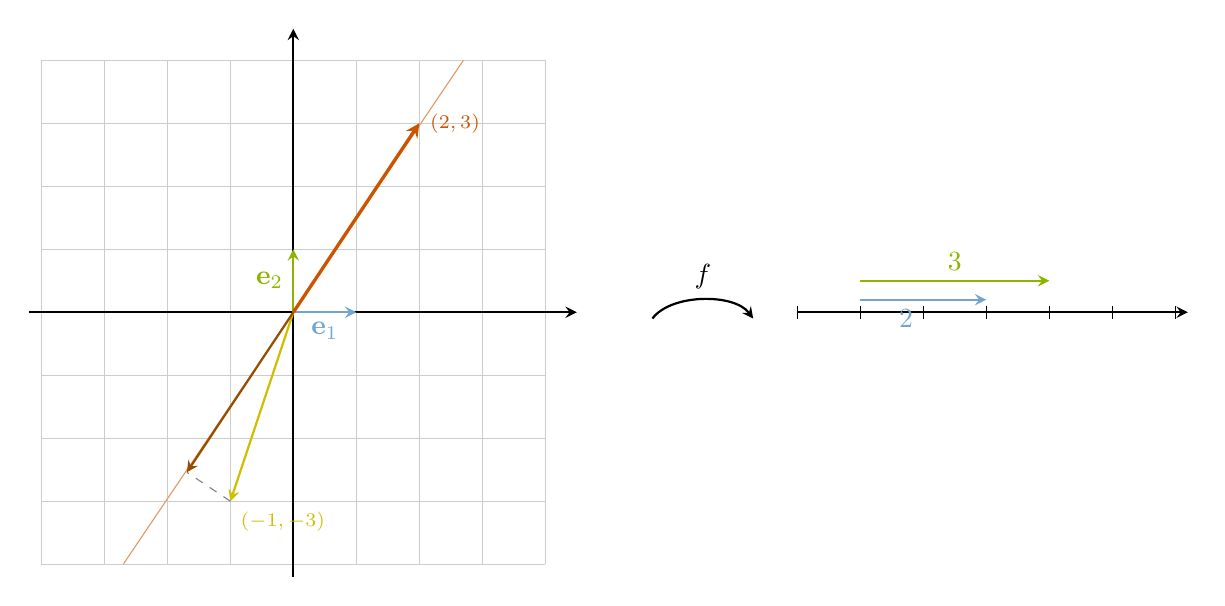
\begin{tikzpicture}[scale=0.8,>=stealth]
\begin{scope}[shift={(0,0)}]
    % Draw 2D grid
    \draw[step=1cm,gray!40,thin] (-4,-4) grid (4,4);

    % Axes
    \draw[thick,->] (-4.2,0) -- (4.5,0);
    \draw[thick,->] (0,-4.2) -- (0,4.5);

    % Basis vectors
    \draw[->,thick,iceberg] (0,0) -- (1,0) node[midway,below] {$\bfe_1$};
    \draw[->,thick,applegreen] (0,0) -- (0,1) node[midway,left] {$\bfe_2$};

    % 1D subspace spanned by (2,3)
    \draw[thin,burntorange!60] (-2.7,-4) -- (2.7,4); % the whole line
    \draw[->,very thick,burntorange] (0,0) -- (2,3) node[right] {\scriptsize{$(2,3)$}};

    % Vector v = (-1,-3)
    \draw[->,thick,canaryyellow!80!black] (0,0) -- (-1,-3) node[below right] {\scriptsize{$(-1,-3)$}};

    % Projection of v onto span{(2,3)}
    \coordinate (proj) at (-1.69,-2.54);
    \draw[dashed,gray] (-1,-3) -- (proj); % projection drop line
    \draw[->,thick,orange!60!black] (0,0) -- (proj) node {};
\end{scope}

% Curved arrow labelled f
\begin{scope}[shift={(4,-.4)}]
    \draw[->, thick]
        (1.7,0.3) .. controls (2,0.7) and (3,0.7) .. (3.3,0.3)
        node[midway, above] {$f$};
\end{scope}

% 1D grid (real line)
\begin{scope}[shift={(9,0)}]
    % Real line
    \draw[step=1cm,gray!40,thin] (-1,0) grid (5,0);
    \draw[thick,->] (-1,0) -- (5.2,0) node {};

    % Ticks (no labels)
    \foreach \x in {-1,0,1,2,3,4,5}
        \draw (\x,0.1) -- (\x,-0.1);

    % Vectors (as arrows on the real line)
    \draw[->,thick,iceberg] (0,0.2) -- (2,0.2) node[midway,below left] {$2$};
    \draw[->,thick,applegreen] (0,0.5) -- (3,0.5) node[midway,above] {$3$};
\end{scope}
\end{tikzpicture}
\]
Το $f(-1,-3)$ ισούται με το μήκος του $(2,3)$ πολλαπλασιασμένο με το μήκος της προβολής του $(-1,-3)$ στην ευθεία που παράγεται από το $(2,3)$. Με άλλα λόγια, το εσωτερικό τους γινόμενο.

Το σύνολο $V^\ast \coloneqq \Hom(V,\FF)$ ονομάζεται \defn{δυϊκός χώρος} του $V$. Το Θεώρημα του Riesz μας πληροφορεί ότι αν το $\FF$ είναι το $\RR$ ή το $\CC$, τότε η απεικόνιση 
\begin{align*}
    V &\to V^\ast \\
    v &\mapsto \Arg \cdot v
\end{align*}
είναι αμφιμονοσήμαντη. Στην περίπτωση όπου $\FF = \RR$, τότε η γραμμικότητα του εσωτερικού γινομένου έχει ως συνέπεια η απεικόνιση αυτή να είναι γραμμικός ισομορφισμός και γι' αυτό $V \cong V^\ast$. Στην περίπτωση όπου $\FF = \CC$ θέλει μια προσοχή, καθώς το εσωτερικό γινόμενο είνια \emph{συζυγές γραμμικό} ως προς τη δεύτερη μεταβλητή και γι' αυτό ο δυϊκός χώρος είναι (ουσιαστικά) ο $V$, αλλά με διαφορετική δομή γραμμικότητας. Σε γενικότερες περιπτώσεις, αυτές οι δύο ταυτίσεις παύουν να ισχύουν, αλλά $V \cong \left(V^\ast\right)^\ast$.

Από την παραπάνω συζήτηση, δοθήσεις μια βάσης $\{v_1, v_2, \dots, v_n\}$ του $V$ προκύπτει μια φυσική βάση του δυϊκού χώρου. Αυτή αποτελείται από τις \emph{προβολές} στην ευθεία που παράγεται από τo $v_i$. Πιο συγκεκριμένα, το σύνολο $\{v_1^\ast, v_2^\ast, \dots, v_n^\ast\}$ όπου 
\begin{align*}
    v_i^\ast : V &\to \RR \\
    v_j &\mapsto 
    \begin{cases}
        1, &\ \text{αν $i =j$} \\
        0, &\ \text{διαφορετικά}
    \end{cases}
\end{align*}
για κάθε $1 \le i \le n$ αποτελεί βάση του $V^\ast$ (γιατί;) η οποία ονομάζεται \emph{δυϊκή βάση} της $\{v_1, v_2, \dots, v_n\}$.
\end{digression_la}

\begin{proof}[Απόδειξη του Θεωρήματος~\ref{thm:vdual_tensor_w_cong_homvw}]
    Αρχικά, παρατηρούμε ότι η απεικόνιση $V^\ast \times W \to \Hom(V,W)$ που ορίζεται θέτοντας
    \[
    (f, w)(v) \mapsto f(v)w
    \]
    για κάθε $v \in V, f \in V^\ast$ και $w \in W$
    είναι διγραμμική και γι' αυτό από το Θεώρημα \ref{thm:tensor_product_universal_property} επάγεται η γραμμική απεικόνιση $\Gamma$. Θα δείξουμε ότι η $\Gamma$ είναι γραμμικός ισομορφισμός και $G$-ομομορφισμός.

    Για τον πρώτο ισχυρισμό, αρκεί να δείξουμε ότι η $\Gamma$ στέλνει μια βάση του $V^\ast \otimes W$ σε μια βάση του $\Hom(V,W)$. Έστω $\{v_1, v_2, \dots, v_n\}$ και $\{w_1, w_2, \dots, w_m\}$ βάσεις των $V$ και $W$, αντίστοιχα. Από το Θεώρημα~\ref{thm:tensor_product_basis}, το σύνολο 
    \[
    \{v_i^\ast \otimes w_j : 1 \le i \le n, \ 1 \le j \le m\}
    \]
    αποτελεί βάση του $V^\ast \otimes W$ (γιατί;). Η εικόνα ενός αυθαίρετου στοιχείου της βάσης αυτής μέσω της $\Gamma$ είναι 
    \[
    \Gamma(v_i^\ast \otimes w_j)(v_k) = v_i^\ast(v_j)w_k =
    \begin{cases}
    w_j, &\ \text{αν $i=k$} \\ 
    0,   &\ \text{διαφορετικά}
    \end{cases}
    \]
    το οποίο δεν είναι άλλο από εκείνη την γραμμική απεικόνιση $\varphi_{ij}$ που συναντήσαμε πριν το Θεώρημα~\ref{thm:vdual_tensor_w_cong_homvw} και το ζητούμενο έπεται.

    Για το δεύτερο, αρκεί να επαληθεύσουμε την Ταυτότητα \eqref{eq:representation_homomorphism}, δηλαδή 
    \[
    \Gamma\left(\underbrace{g\cdot(f\otimes{w})}_{\text{δράση της $G$ στο $V^\ast \otimes W$}}\right) = 
    \underbrace{g\cdot\Gamma(f\otimes{w})}_{\text{δράση της $G$ στο $\Hom(V,W)$}},
    \]
    για κάθε $g \in G, f \in V^\ast$ και $w \in W$. Πράγματι, για κάθε $v \in V$, 
    \begin{align*}
    \Gamma\left(g\cdot(f\otimes{w})\right)(v) &= 
    \Gamma\left(\underbrace{g\cdot{f}}_{\text{δράση της $G$ στο $V^\ast$}} \otimes \underbrace{g\cdot{w}}_{\text{δράση της $G$ στο $W$}}\right)(v) \\ 
    &= (g\cdot{f})(v)g\cdot{w} \\
    &= f(g^{-1}v) \, gw.
    \end{align*}
    Από την άλλη, 
    \begin{align*}
        \left(g\cdot\Gamma(f\otimes{w})\right) (v)
        &= \underbrace{g\cdot\left(\Gamma(f\otimes{w})(\underbrace{g^{-1}\cdot{v}}_{\text{δράση της $G$ στο $V$}})\right)}_{\text{δράση της $G$ στο $W$}} \\
        &= g\cdot\left(f(g^{-1}\cdot{v}) \, w\right) \\ 
        &= f(g^{-1}v) \, gw,
    \end{align*}
    και το ζητούμενο έπεται.
\end{proof}

Συνεπώς, ξεκινώντας από δύο διανυσματικούς χώρους, έχουμε κατασκευάσει τα εξής $G$-πρότυπα 
\[
V \oplus W, \, V\otimes{W}, \, \Hom(V,W), \ \text{και} \ V^\ast.
\]
Ας υπολογίσουμε τους χαρακτήρες τους και πως σχετίζονται με αυτούς των $V$ και $W$.
\begin{proposition}
    \label{prop:characters_of_constructions}
    Αν $V$ και $W$ είναι δύο $G$-πρότυπα πεπερασμένης διάστασης, τότε 
    \begin{align}
        \chi^{V\oplus{W}} &= \chi^V + \chi^W \label{eq:character_direct_sum}\\
        \chi^{V\otimes{W}} &= \chi^V\chi^W \label{eq:character_tensor_product}\\
        \chi^{V^\ast} &= \ol{\chi^V} \label{eq:character_dual} \\
        \chi^{\Hom(V,W)} &= \ol{\chi^V}\chi^W, \label{eq:character_hom}
    \end{align}
    όπου $\ol{\chi^V} : G \to \CC$ ορίζεται θέτοντας $\ol{\chi^V}(g) = \ol{\chi^V(g)}$ για κάθε $g \in G$.
\end{proposition}

\begin{proof}[Απόδειξη]
    Έστω $(\rho, V)$ και $(\sigma, W)$ οι αντίστοιχες αναπαραστάσεις της $G$ και έστω $\{v_1, v_2,$ $\dots, v_n\}$, $\{w_1, w_2, \dots, w_m\}$ βάσεις των $V$ και $W$, αντίστοιχα. Για την Ταυτότητα \eqref{eq:character_direct_sum}, αρκεί να παρατηρήσουμε ότι ο πίνακας της δράσης του $g$ στο $V \oplus W$ έχει την μορφή
    \[
    \begin{pmatrix}
        \rho(g) & 0 \\
        0       & \sigma(g)
    \end{pmatrix}
    \]
    (γιατί;). 
    
    Για την Ταυτότητα \eqref{eq:character_tensor_product}, από το Θεώρημα \ref{thm:tensor_product_basis} το σύνολο $\{v_i \otimes w_j : 1 \le i \le n, \, 1 \le j \le m\}$ αποτελεί βάση του $V \otimes W$. Πρέπει να υπολογίσουμε τον πίνακα του $\rho(g)$ ως προς αυτή τη βάση. Αν 
    \[
    \rho(g) = (\alpha_{ij})_{1 \le i, j \le n} \quad \text{και} \quad \sigma(g) = (\beta_{ij})_{1 \le i,j \le m}
    \]
    τότε 
    \begin{align*}
        g \cdot (v_i \otimes w_j)
        &= \rho(g)(v_i) \otimes \sigma(g)(w_j) \\
        &= \left(
            \alpha_{1i}v_1 + \cdots + \alpha_{ni}v_n 
        \right) \otimes 
        \left(
            \beta_{1j}w_1 + \cdots + \beta_{mj}w_m
        \right) \\ 
        &= \sum_{\substack{1 \le k \le n \\ 1 \le \ell \le m}} \alpha_{ki}\beta_{\ell{j}} \, v_k \otimes w_\ell,
    \end{align*}
    για κάθε $ 1 \le i \le n$ και $1 \le j \le m$. Με άλλα λόγια, ο πίνακας της δράσης του $g$ στο $V\otimes{W}$ είναι το γινόμενο Kronecker των $\rho(g)$ και $\sigma(g)$ και γι' αυτό
    \begin{align*}
        \chi^{V\otimes{W}}(g) 
        &= \sum_{i=1}^n \left(\alpha_{ii}\left(\sum_{j=1}^m\beta_{jj}\right)\right) \\
        &= \left(\sum_{i=1}^n\alpha_{ii}\right)\left(\sum_{j=1}^m\beta_{jj}\right) \\
        &= \trace(\rho(g))\trace(\sigma(g)) \\
        &= \chi^V(g)\chi^W(g),
    \end{align*}
    και το ζητούμενο έπεται.    

    Για την Ταυτότητα \eqref{eq:character_dual}, πρέπει να υπολογίσουμε τον πίνακα του $\rho(g)$ ως προς αυτή τη δυϊκή βάση $\{v_1^\ast, v_2^\ast, \dots, v_n^\ast\}$. Υποθέτουμε ότι  
    \[
    \rho(g^{-1}) = 
    \begin{pmatrix}
        \gamma_{11} & \gamma_{12} & \cdots & \gamma_{1n} \\
        \gamma_{21} & \gamma_{22} & \cdots & \gamma_{2n} \\
        \vdots      & \vdots      &        & \vdots \\
        \gamma_{n1} & \gamma_{n2} & \cdots & \gamma_{nn} \\
    \end{pmatrix}
    \]
    για $g \in G$ και γι αυτό
    \[
    \rho(g^{-1})(v_i) = \gamma_{1i}v_1 + \gamma_{2i}v_2 + \cdots + \gamma_{ni}v_n.
    \]
    Συνεπώς,
    \[
    \left(g \cdot v_j^\ast\right)(v_i) 
    = v_j^\ast\left(\rho(g^{-1})(v_i)\right) 
    = v_j^\ast(\gamma_{1i}v_1 + \gamma_{2i}v_2 + \cdots + \gamma_{ni}v_n) 
    = \gamma_{ji}
    \]
    για κάθε $1 \le i, j \le n$. Με άλλα λόγια ο πίνακας της δράσης του $g$ στο $V^\ast$ είναι ο ανάστροφος του $\rho(g^{-1})$ και γι αυτό 
    \[
    \chi^{V^\ast}(g) = \trace\left(\rho(g^{-1})^\top\right) = \chi^V(g^{-1}) = \ol{\chi^V(g)},
    \]
    όπου η τελευταία ισότητα έπεται από την Άσκηση~2.2~(2).

    Τέλος, η Ταυτότητα \eqref{eq:character_hom} έπεται από τις Ταυτότητες \eqref{eq:character_tensor_product} και \eqref{eq:character_dual}, σε συνδυασμό με το Θεώρημα \ref{thm:vdual_tensor_w_cong_homvw} και την Πρόταση \ref{prop:character_properties}~(3). 
\end{proof}

Οι πρώτες δύο ταυτότητες της Πρότασης \ref{prop:characters_of_constructions} μας πληροφορούν ότι το άθροισμα και το γινόμενο δύο χαρακτήρων είναι και αυτοί χαρακτήρες κάποιων αναπαραστάσεων, γεγονός το οποίο δεν είναι καθόλου προφανές εκ των προτέρων.
\begin{example}
    \label{ex:standard_representation}
    Από την συζήτηση της Πραγράφου \ref{sec:maschke}, προκύπτει η εξής διάσπαση
    \begin{align}
    V^{\rmdef} &= \CC[\bfe_1 + \cdots + \bfe_n] \oplus \left(\CC[\bfe_1 + \cdots + \bfe_n]\right)^\perp \notag \\
    &= \underbrace{\CC[\bfe_1 + \cdots + \bfe_n]}_{\cong \, V^{\triv}} \oplus \underbrace{\CC[\bfe_1-\bfe_2, \bfe_1 - \bfe_3, \dots, \bfe_1 - \bfe_n]}_{\coloneqq \, V^{\std}} \label{eq:def_isotypic}
    \end{align}
    $\fS_n$-προτύπων. Η αναπαράσταση $V^\std$ ονομάζεται \defn{συνήθης} (standard) αναπαράσταση της $\fS_n$ και έχει διάσταση $n-1$. Από την Ταυτότητα \eqref{eq:character_direct_sum}, ο χαρακτήρας της είναι 
    \[
    \chi^\std(\pi) = \fix(\pi) - 1,
    \]
    για κάθε $\pi \in \fS_n$.

    Θα αποδείξουμε ότι το $V^\std$ είναι \emph{ανάγωγo} πρότυπο και κατά συνέπεια, η Διάσπαση~\eqref{eq:def_isotypic} είναι η ισοτυπική διάσπαση της αναπαράστασης καθορισμού. Έστω $v = (v_1, v_2, \dots, v_n) \in V^\std$ τέτοιο ώστε $v \neq 0$. Θα δείξουμε ότι ο υπόχωρος που παράγεται από την τροχιά του $v$ περιέχει τα στοιχεία $\bfe_1 - \bfe_2, \bfe_1 - \bfe_3, \dots, \bfe_1-\bfe_n$ και κατά συνέπεια ολόκληρο τον $V^\std$. Με άλλα λόγια, ο $V^\std$ δεν περιέχει γνήσιους $\fS_n$-αναλλοίωτους υπόχωρους διαφορετικούς από το $\{0\}$. 

    Πράγματι, αφού $v \neq 0$ έπεται ότι  $v_i \neq v_{i+1}$ για κάποιο $1 \le i \le n-1$ (γιατί;). Αν $s_j \coloneqq \cycle{j,j+1}$ είναι η αντιμετάθεση που εναλλάσει τα $j$ και $j+1$ και αφήνει όλα τα άλλα σταθερά για κάθε $1 \le j \le n-1$, τότε 
    \[ 
    s_i\cdot{v} = (v_1, \dots, v_{i+1}, v_i, \dots, v_n)
    \]
    (γιατί;) και γι' αυτό 
    \begin{align*}
    v - s_i\cdot{v} 
    &= (0, \dots, \underbrace{v_i - v_{i+1}}_{\text{$i$-οστή θέση}}, \underbrace{v_{i+1} - v_i}_{\text{$(i+1)$-οστή θέση}}, \dots, 0) \\ 
    &= \underbrace{(v_i - v_{i+1})}_{\neq \, 0}(\bfe_i - \bfe_{i+1}).
    \end{align*}
    Άρα, $\bfe_i - \bfe_{i+1} \in \CC[\oO_v]$ και κατά συνέπεια 
    \[
    \bfe_1 - \bfe_{i+1} = (s_1s_2\cdots{s_{i-1}})\cdot{\bfe_i - \bfe_{i+1}} \in \oO_v
    \]
    (γιατί;) και 
    \[
    \bfe_1 - \bfe_k = 
    \begin{cases}
        (s_ks_{k+1}\cdots s_i)(\bfe_1-\bfe_{i+1}), &\ \text{αν $2\le k \le i$} \\ 
        (s_ks_{k+1}\cdots s_{i+1})(\bfe_1-\bfe_{i+1}), &\ \text{αν $i+1 \le k \le n$} \\ 
    \end{cases} \quad \in \oO_v,
    \]
    που ήταν το ζητούμενο. Τώρα, μπορούμε να ολοκληρώσουμε τον πίνακα χαρακτήρων της $\fS_3$
    \renewcommand{\arraystretch}{1.2} 
    \[
    \begin{array}{l|c|c|c}
                   & \rmK_{111} & \rmK_{21} & \rmK_3 \\ \hline
        \chi^\triv & 1       & 1      & 1 \\ \hline
        \chi^\sign & 1       & -1     & 1 \\ \hline
        \chi^\std  & 2       & 0      & -1 
    \end{array} \ .
    \]
\end{example}

\section{Χαρακτήρες ομάδων: Σχέσεις ορθογωνιότητας}
\label{sec:characters_orthogonality_relations}

Στην παράγραφο αυτή θα χρησιμοποιήσουμε τα αποτελέσματα των προηγούμενων παραγράφων για να απαντήσουμε στα δύο από τα τρία ερωτήματα που τέθηκαν στην Παράγραφο \ref{sec:regular_representation}. Σε ότι ακολουθεί υποθέτουμε ότι $G$ είναι μια πεπερασμένη ομάδα και όλοι οι διανυσματικοί χώροι είναι πεπερασμένης διάστασης πάνω από το $\CC$.

Ας θυμηθούμε τον πίνακα χαρακτήρων της $\rmC_3$
\renewcommand{\arraystretch}{1.2}
\[
\begin{array}{l|c|c|c}
           & \{\epsilon\} & \{g\}   & \{g^2\} \\ \hline
    \chi_1 & 1            & 1       & 1 \\ \hline
    \chi_2 & 1            & \zeta   & \zeta^2 \\ \hline
    \chi_3 & 1            & \zeta^2 & \zeta
\end{array}\ ,
\]
όπου $\zeta$ είναι μια τρίτη ρίζα της μονάδας. Αν φανταστούμε τους ανάγωγους χαρακτήρες της $\rmC_3$ ως διανύσματα του $\CC^3$, δηλαδή
\[
\chi_1 = (1,1,1), \quad \chi_2=(1,\zeta,\zeta^2), \quad \text{και} \quad \chi_3 = (1,\zeta^2,\zeta),
\]
και υπολογίσουμε το εσωτερικό τους γινόμενο, τότε παρατηρούμε ότι 
\begin{align*}
\chi_1\cdot\chi_2 &= \chi_1\cdot\chi_3 = \chi_2\cdot\chi_3 = 0 \\
\chi_1\cdot\chi_1 &= \chi_2\cdot\chi_2 = \chi_3\cdot\chi_3 = 3. 
\end{align*}
Με άλλα λόγια, το σύνολο $\{\chi_1, \chi_2, \chi_3\}$ είναι ορθογώνιο ως προς το σύνηθες εσωτερικό γινόμενο του $\CC^3$. Η παρατήρηση αυτή μας οδηγεί στον εξής ορισμό.
\begin{definition}
    \label{def:character_inner_product}
    Για δύο συναρτήσεις $\alpha, \beta : G \to \CC$ (όχι απαραίτητα χαρακτήρες της $G$), θέτουμε 
    \begin{equation}
    \label{eq:character_inner_product_def}
    (\alpha, \beta)_G \coloneqq  \frac{1}{\abs{G}} \sum_{g \in G} \alpha(g)\ol{\beta(g)},
    \end{equation}
    ή απλούστερα $(\alpha, \beta)$.
\end{definition}
Η απεικόνιση $(\Arg, \Arg)$ είναι εσωτερικό γινόμενο στον χώρο των συναρτήσεων κλάσης $\rmCF(G)$ (γιατί;). Από την Άσκηση~2.2~(2), αν $\chi$ και $\psi$ είναι δύο χαρακτήρες της $G$, τότε 
\begin{equation}
    \label{eq:character_bilinear}
    (\chi, \psi)_G = \frac{1}{\abs{G}} \sum_{g \in G} \chi(g)\psi(g^{-1}).
\end{equation}
Αν ορίζαμε το $(\Arg,\Arg)$ από το δεξί μέλος της Ταυτότητας~\eqref{eq:character_bilinear}, αντί γι αυτό της Ταυτότητας~\eqref{eq:character_inner_product_def}, τότε θα είχαμε μια διγραμμική απεικόνιση $\rmCF(G) \times \rmCF(G) \to \CC$, αντί για εσωτερικό γινόμενο. Παρόλα αυτά, στους χαρακτήρες της $G$ οι δύο τύποι συμφωνούν.

\begin{theorem}
    \label{thm:inner_prod_of_characters}
    Αν $V, W$ είναι δύο $G$-πρότυπα, τότε 
    \begin{equation}
        \label{eq:inner_prod_of_characters}
        (\chi^V,\chi^W) = \dim\left(\Hom_G(W,V)\right) = \dim\left(\Hom_G(V,W)\right).
    \end{equation}
\end{theorem}

Η Ταυτότητα~\eqref{eq:inner_prod_of_characters} εξηγεί την συμμετρία που παρατηρήσαμε μετά το Λήμμα \ref{lem:Schur_uniqueness_of_isotypic_decomposition}. Η απόδειξη του Θεωρήματος~\ref{thm:inner_prod_of_characters} βασίζεται στο παρακάτω αποτέλεσμα, την βασική ιδέα του οποία συναντήσαμε στην απόδειξη της Πρότασης \ref{prop:weyl_unitary_trick}.

\begin{lemma}
    \label{lem:projection}
    Έστω $(\rho,V)$ μια αναπαράσταση της $G$ και 
    \[
    V^G \coloneqq \{v \in V : \rho(g)(v) = v, \, \text{για κάθε $g \in G$}\}.
    \]
    \begin{itemize}
        \item[(1)] Το $V^G$ είναι υποαναπαράσταση της $V$.
        \item[(2)] Η απεικόνιση $\tl{\rho} : V \to V$ που ορίζεται θέτοντας 
        \[
        \tl{\rho}(v) = \frac{1}{\abs{G}} \sum_{g \in G} \rho(g)(v)
        \]
        για κάθε $v \in V$ είναι $G$-ομομορφισμός.
        \item[(3)] Ισχύει ότι $\mathrm{Im}(\tl{\rho}) = V^G$.
        \item[(4)] Ισχύει ότι 
        \[
        \dim(V^G) = \frac{1}{\abs{G}}\sum_{g \in G} \chi^{\rho,V}(g).
        \]
    \end{itemize}
\end{lemma}

\begin{proof}[Απόδειξη]
    Για το (1), αν $x \in G$ και $v \in V^G$, τότε για κάθε $g \in G$
    \[
    \rho(g)\left(\rho(x)(v)\right) = \rho(gx)(v) = v,
    \]
    όπου η πρώτη ισότητα έπεται από το ότι η $\rho$ είναι ομομορφισμός ομάδων και η δεύτερη ισότητα από το ότι $v \in V^G$. Συνεπώς, το $V^G$ είναι $G$-αναλλοίωτο.

    Για το (2), η γραμμικότητα της $\tl{\rho}$ έπεται άμεσα από την γραμμικότητα της $\rho$. Για να δείξουμε ότι είναι $G$-ομομορφισμός, πρέπει να δείξουμε ότι 
    \[
    \tl{\rho}\left(\rho(x)(v)\right) = \rho(x)\left(\tl{\rho}(v)\right) 
    \]
    ή ισοδύναμα ότι 
    \[
    \rho(x^{-1})\left(\tl{\rho}\left(\rho(x)(v)\right)\right) = \tl{\rho}(v)
    \]
    για κάθε $x\in G$ και $v \in V$. Πράγματι, 
    \begin{align*}
        \rho(x^{-1})\left(\tl{\rho}\left(\rho(x)(v)\right)\right) 
        &= \rho(x^{-1})\left(
            \frac{1}{\abs{G}} \sum_{g \in G} \rho(g)\left(\rho(x)(v)\right)
        \right) \\ 
        &= \frac{1}{\abs{G}} \sum_{g \in G} \rho(x^{-1})\left(\rho(g)\left(\rho(x)(v)\right)\right) \\
        &= \frac{1}{\abs{G}}\sum_{g \in G} \rho(x^{-1}gx)(v) \\
        &= \frac{1}{\abs{G}}\sum_{h \in G} \rho(h)(v) \\
        &= \tl{\rho}(v),
    \end{align*}
    όπου η δεύτερη (αντ. τρίτη) ισότητα έπεται από το ότι η $\rho$ είναι γραμμική απεικόνιση (αντ. ομομορφισμός ομάδων) και η τέταρτη από αλλαγή μεταβλητής $h \to x^{-1}gx$ στο άθροισμα.

    Για το (3), αν $v \in \mathrm{Im}(\tl{\rho})$, τότε $v = \tl{\rho}(v_0)$, για κάποιο $v_0 \in V$ και γι αυτό 
    \begin{align*}
        \rho(x)(\tl{\rho}(v_0)) 
        &= \rho(x)\left(\frac{1}{\abs{G}} \sum_{g \in G} \rho(g)(v_0)\right) \\
        &= \frac{1}{\abs{G}} \sum_{g \in G} \rho(x)\left(\rho(g)(v_0)\right) \\ 
        &= \frac{1}{\abs{G}} \sum_{g \in G} \rho(xg)(v_0) \\ 
        &= \frac{1}{\abs{G}}\sum_{h \in G} \rho(h)(v_0) \\
        &= \tl{\rho}(v_0)
    \end{align*}
    για κάθε $x \in G$, όπου η δεύτερη (αντ. τρίτη) ισότητα έπεται από το ότι η $\rho$ είναι γραμμική απεικόνιση (αντ. ομομορφισμός ομάδων) και η τέταρτη από αλλαγή μεταβλητής $h \to xg$ στο άθροισμα. Άρα, $v \in V^G$ και γι' αυτό $\mathrm{Im}(\tl{\rho}) \subseteq V^G$. Για τον άλλο εγκλεισμό, αν $v \in V^G$, τότε
    \[
    \tl{\rho}(v) = \frac{1}{\abs{G}}\sum_{g \in G} \rho(g)(v) = \frac{1}{\abs{G}} \sum_{g \in G} v = v
    \]
    που σημαίνει ότι $v \in \mathrm{Im}(\tl{\rho})$ και γι αυτό $V^G \subseteq \mathrm{Im}(\tl{\rho})$.

    Τέλος, για το (4), παρατηρούμε ότι η $\tl{\rho}$ είναι \emph{προβολή}, δηλαδή $\tl{\rho}\circ\tl{\rho} = \tl{\rho}$. Πράγματι,
    \begin{align*}
        \tl{\rho}\left(\tl{\rho}(v)\right)
        &= \tl{\rho}\left(\frac{1}{\abs{G}} \sum_{g \in G} \rho(g)(v)\right) \\
        &= \frac{1}{\abs{G}} \sum_{g \in G} \tl{\rho}\left(\rho(g)(v)\right) \\
        &= \frac{1}{\abs{G}} \sum_{g \in G} \rho(g)\left(\tl{\rho}(v)\right) \\
        &=\tl{\rho}(v),
    \end{align*}
    όπου η δεύτερη ισότητα έπεται από την γραμμικότητα της $\tl{\rho}$ και η τρίτη (αντ. τέταρτη) ισότητα έπεται από το (2) (αντ. (3)). Αυτό έχει ως συνέπεια\footnote{Γενικότερα, αν έχουμε μια προβολή $p : V\to{V}$ σε ένα διανυσματικό χώρο $V$, τότε $V = \mathrm{Im}(p) \oplus \Ker(p)$.},
    \[
    V = \mathrm{Im}(\tl{\rho}) \oplus \Ker(\tl{\rho}),
    \]
    και γι αυτό ο πίνακας του $(\tl{\rho})$ έχει την εξής μορφή 
    \[
    \begin{pmatrix}
        \mathrm{I}_{\dim(\mathrm{Im}(\tl{\rho}))} & 0 \\ 
        0 & 0
    \end{pmatrix},
    \]
    όπου $\mathrm{I}_k$ είναι ο ταυτοτικός $(k\times{k})$-πίνακας. 
    Υπολογίζοντας το ίχνος του έπεται ότι 
    \[
    \dim(V^G) = \dim(\mathrm{Im}(\tl{\rho})) = \trace\left(\tl{\rho}\right) = \frac{1}{\abs{G}} \sum_{g \in G} \trace\left(\rho(g)\right) = \frac{1}{\abs{G}}\sum_{g \in G} \chi^{\rho,V}(g),
    \]
    όπου η πρώτη ισότητα έπεται από το (3), και η απόδειξη ολοκληρώθηκε.
\end{proof}

\begin{proof}[Απόδειξη του Θεωρήματος~\ref{thm:inner_prod_of_characters}]
    Για την πρώτη ισότητα της Ταυτότητας~\ref{eq:inner_prod_of_characters},
    \begin{align*}
        (\chi^V,\chi^W) 
        &= \frac{1}{\abs{G}}\sum_{g\in{G}} \chi^V(g)\ol{\chi^W(g)} \\ 
        &= \frac{1}{\abs{G}}\sum_{g\in{G}}\chi^{\Hom(W,V)}(g) \\ 
        &= \dim\left(\Hom(W,V)^G\right) \\
        &= \dim\left(\Hom_G(W,V)\right),
    \end{align*}
    όπου η δεύτερη ισότητα έπεται από την Ταυτότητα \eqref{eq:character_hom}, η τρίτη ισότητα έπεται από το Λήμμα~\ref{lem:projection} και η τέταρτη ισότητα από την Άσκηση~1.4~(2).

    Για την δεύτερη ισότητα της Ταυτότητας~\ref{eq:inner_prod_of_characters},
    \[
    (\chi^V,\chi^W) = \ol{(\chi^V,\chi^W)} = (\chi^W,\chi^V) = \dim\left(\Hom_G(V,W)\right),
    \]
    όπου η πρώτη ισότητα έπεται από την συζυγή συμμετρία του εσωτερικού γινομένου.
\end{proof}

Συνδυάζοντας το Θεώρημα~\ref{thm:inner_prod_of_characters} και το Πόρισμα \ref{cor:schur_dimension_of_Hom_space} προκύπτει ότι το σύνολο των ανάγωγων χαρακτήρων της $G$ είναι ορθοκανονικό ως προς το εσωτερικό γινόμενο που ορίσαμε.

\begin{theorem}{\rm(Σχέσεις ορθογωνιότητας Ι)}
    \label{thm:orthogonality_rels_I}
    Αν $V$ και $W$ είναι ανάγωγα $G$-πρότυπα, τότε 
    \[
    (\chi^V,\chi^W) = 
    \begin{cases}
        1, &\ \text{αν $V\cong_G{W}$} \\
        0, &\ \text{διαφορετικά}
    \end{cases}.
    \]
\end{theorem}

\begin{corollary}
    \label{cor:orthogonality_rels_I}
    Αν $V$ είναι $G$-πρότυπο με ισοτυπική διάσπαση 
    \[
    V = V_1^{m_1} \oplus V_2^{m_2} \oplus \cdots \oplus V_n^{m_n},
    \]
    όπου $\{V_1, V_2, \dots, V_n\}$ είναι ένα σύνολο ανά δύο μη ισόμορφων $G$-προτύπων, τότε 
    \begin{itemize}
        \setlength{\itemsep}{4pt}
        \item[(1)] $\chi^V = m_1\chi^{V_1} + m_2\chi^{V_2} + \cdots + m_n\chi^{V_n}$,
        \item[(2)] $(\chi^V,\chi^{V_i}) = m_i$, για κάθε $1 \le i \le n$,
        \item[(3)] $(\chi^V,\chi^V) = m_1^2 + m_2^2 + \cdots + m_n^2$.
    \end{itemize}
    Ειδικότερα, το $V$ είναι ανάγωγο αν και μόνο αν $(\chi^V,\chi^V) = 1$.
\end{corollary}

\begin{proof}[Απόδειξη]
    Το (1) έπεται άμεσα από την Ταυτότητα \eqref{eq:character_direct_sum}. Για το (2), υπολογίζουμε
    \[
    (\chi^V, \chi^{V_i}) = (\left(\sum_{j=1}^n m_j \chi^{V_j}\right), \chi^{V_i}) = \sum_{j=1}^n m_j \, (\chi^{V_j}, \chi^{V_i}) = m_i 
    \]
    όπου η τελευταία ισότητα έπεται από το Θεώρημα \ref{thm:orthogonality_rels_I}. Για το (3), υπολογίζουμε 
    \[
    (\chi^V, \chi^V) = \left(\left(\sum_{i=1}^n m_i \chi^{V_i}\right), \left(\sum_{j=1}^n m_j \chi^{V_j}\right)\right) 
    = \sum_{1 \le i, j \le n} m_i\ol{m_j} \, (\chi^{V_i}, \chi^{V_j}) 
    = \sum_{i=1}^n m_i^2,
    \]
    όπου η τελευταία ισότητα έπεται από το Θεώρημα \ref{thm:orthogonality_rels_I}. 
    
    Τέλος, το $V$ είναι ανάγωγο $G$-πρότυπο αν και μόνο αν υπάρχει μοναδικό $1 \le i \le n$ για το οποίο $m_i = 1$ και $m_j = 0$ για κάθε $j \neq i$, ή ισοδύναμα, από το (3), αν και μόνο αν $(\chi^V, \chi^V)=1$. 
\end{proof}

Το Πόρισμα \ref{cor:orthogonality_rels_I} μας δίνει ένα ισχυρό κριτήριο για το πότε ένα $G$-πρότυπο είναι ανάγωγο. Για παράδειγμα, ξεχνώντας προσωρινά το Παράδειγμα \ref{ex:standard_representation}, μπορούμε να δείξουμε ότι η συνήθης αναπαράσταση της $\fS_3$ είναι ανάγωγη υπολογίζοντας το $(\chi^\std, \chi^\std)$. Πράγματι, 
    \[
    \renewcommand{\arraystretch}{1.2} 
    \begin{array}{c|c|c|c}
              & \rmK_{111} & \rmK_{21} & \rmK_{3} \\ \hline
    \chi^\std & 2          & 0       & -1        
    \end{array}
    \]
και γι αυτό 
    \[
    (\chi^\std, \chi^\std) = \frac{1}{6}(2^2 + 3\cdot0 + 2\cdot(-1)^2) = 1,
    \]
όπως περιμέναμε.
Τι γίνεται για μεγαλύτερα $n$ (βλ. Άσκηση 2.4);

Ομοίως, για την αναπαράσταση $\rho$ της Άσκησης 1.4, υπολογίζουμε 
    \[
    \renewcommand{\arraystretch}{1.2} 
    \begin{array}{c|c|c|c|c|c}
              & \{\epsilon\} & \{r^2\} & \{r, r^3\} & \{s, sr^2\} & \{sr, sr^3\} \\ \hline
    \chi^\rho & 2            & -2      & 0          & 0           & 0     
    \end{array}
    \]
    και γι αυτό 
    \[
    (\chi^\rho, \chi^\rho) = \frac{1}{8}(2^2 + (-2)^2 + 2\cdot0 + 2\cdot0 + 2\cdot0) = 1.
    \]
Για τον πίνακα χαρακτήρων της $\rmD_{2n}$ δείτε την Άσκηση 2.1.

\begin{corollary}
    \label{cor:representation_isomorphism_criterion}
    Δύο αναπαραστάσεις είναι ισόμορφες αν και μόνο αν έχουν τον ίδιο χαρακτήρα.
\end{corollary}

\begin{proof}[Απόδειξη]
    Την κατεύθυνση \textquote{$\then$} την είδαμε στην Πρόταση \ref{prop:character_properties} (3). Για την άλλη κατεύθυνση, αν δύο πρότυπα έχουν τον ίδιο χαρακτήρα, τότε από το Πόρισμα \ref{cor:orthogonality_rels_I} έπεται ότι τα ανάγωγα πρότυπα που εμφανίζονται στην ισοτυπική τους διάσπαση έχουν τις ίδιες πολλαπλότητες. Τo ζητούμενο έπεται από το Πόρισμα \ref{cor:Schur_uniqueness_of_isotypic_decomposition}.
\end{proof}

Τα Πορίσματα \ref{cor:orthogonality_rels_I} και \ref{cor:representation_isomorphism_criterion} απαντάνε πλήρως στο Ερώτημα (3) της Παραγράφου \ref{sec:regular_representation}. Το επόμενο αποτέλεσμα απαντάει στο Ερώτημα (1).
\begin{theorem}
    \label{thm:character_basis}
    Το σύνολο 
    \[
    \{\chi^V : \ \text{$V$ είναι ανάγωγο $G$-πρότυπο}\}
    \]
    αποτελεί ορθοκανονική βάση του $\rmCF(G)$ ως προς το εσωτερικό γινόμενο $(\Arg,\Arg)_G$. Ειδικότερα, το πλήθος των (διακεκριμένων) ανάγωγων $G$-προτύπων ισούται με το πλήθος των κλάσεων συζυγίας της $G$.
\end{theorem}

Από τις πρώτες σχέσεις ορθογωνιότητας, γνωρίζουμε ότι το σύνολο όλων των $\chi^V $ για ανάγωγα $G$-πρότυπα $V$ είναι ορθοκανονικό και κατά συνέπεια γραμμικώς ανεξάρτητο στο $\rmCF(G)$ (γιατί;). Αρκεί λοιπόν να δείξουμε ότι παράγει τον $\rmCF(G)$. Γι αυτό αρκεί να δέιξουμε ότι το ορθογώνιο συμπλήρωμα του υπόχωρου που παράγει είναι τετριμμένο (γιατί;). Για να το κάνουμε αυτό θα χρησιμοποιήσουμε το εξής.
\begin{lemma}
    \label{lem:character_basis}
    Έστω $(\rho,V)$ μια αναπαράσταση της $G$ και $\alpha \in \rmCF(G)$. 
    \begin{itemize}
        \item[(1)] Η απεικόνιση $\rho_\alpha : V \to V$ που ορίζεται θέτοντας 
        \[
        \rho_\alpha(v) = \frac{1}{\abs{G}} \sum_{g \in G} \ol{\alpha(g)} \rho(g)(v)
        \]
        για κάθε $v \in V$, είναι $G$-ομομορφισμός.
        \item[(2)] Αν η $(\rho, V)$ είναι ανάγωγη, τότε 
        \begin{equation}
            \label{eq:character_basis}
            \rho_\alpha = \frac{(\chi^{\rho,V}, \alpha)}{\dim(V)} \, \rmid_V.
        \end{equation}
    \end{itemize}
\end{lemma}

\begin{proof}[Απόδειξη]
    Για το (1), η γραμμικότητα της $\rho_\alpha$ έπεται από την γραμμικότητα της $\rho$ (γιατί;). Για να επαληθεύσουμε την Ταυτότητα \eqref{eq:representation_homomorphism} για την $\rho_\alpha$ παρατηρούμε ότι 
    \begin{align*}
        \rho(x^{-1})\left(\rho_\alpha(\rho(x)(v))\right)
        &= \frac{1}{\abs{G}} \sum_{g \in G} \ol{\alpha(g)}\rho(x^{-1}gx)(v) \\
        &= \frac{1}{\abs{G}} \sum_{g \in G} \ol{\alpha(x^{-1}gx)}\rho(x^{-1}gx)(v) \\
        &= \frac{1}{\abs{G}} \sum_{h \in G} \ol{\alpha(h)}\rho(h)(v) \\ 
        &= \rho_\alpha(v)
    \end{align*}
    για κάθε $x \in G$ και $v \in V$, όπου η πρώτη ισότητα έπεται από το ότι η $(\rho, V)$ είναι αναπαράσταση, η δεύτερη από το ότι η $\alpha$ είναι συνάρτηση κλάσης και η τρίτη ισότητα προκύπτει από την αλλαγή μεταβλητής $h \to x^{-1}gx$.

    Για το (2), από το Λήμμα του Schur υπάρχει $c \in \CC$ τέτοιο ώστε $\rho_\alpha = c\,\rmid_V$. Υπολογίζοντας το ίχνος και στα δύο μέλη, 
    \begin{align*}
    c \dim(V) 
    &= \trace(\rho_\alpha) \\
    &= \trace\left(\frac{1}{\abs{G}} \sum_{g \in G} \ol{\alpha(g)} \rho(g)(v)\right) \\ 
    &= \frac{1}{\abs{G}} \sum_{g \in G} \ol{\alpha(g)} \chi^{\rho,V}(g) \\
    &= (\chi^{\rho,V}, \alpha),
    \end{align*}
    και το ζητούμενο έπεται.
\end{proof}

\begin{proof}[Απόδειξη του Θεωρήματος \ref{thm:character_basis}]
    Έστω $\alpha \in \rmCF(G)$ τέτοια ώστε $(\alpha, \chi^{\rho,V}) = 0$ ή ισοδύναμα $(\chi^{\rho,V},\alpha) = 0$ για κάθε ανάγωγη ανάγωγη αναπαράσταση $(\rho,V)$ της $G$. Από την Ταυτότητα \eqref{eq:character_basis} έπεται ότι 
    \begin{equation}
        \label{eq:character_basis_proof}
        \sum_{g \in G} \ol{\alpha(G)}\rho(g)(v) = 0,
    \end{equation}
    για κάθε $v \in V$, για κάθε ανάγωγη αναπαράσταση $(\rho,V)$ της $G$. Αφού η Ταυτότητα~\eqref{eq:character_basis_proof} ισχύει για κάθε ανάγωγη αναπαράσταση, θα ισχύει και για κάθε αναπαράσταση της $G$ (γιατί;).

    Για την κανονική αναπαράσταση $(\rho^\reg, \CC[G])$, η Ταυτότητα \eqref{eq:character_basis_proof} γίνεται\footnote{Αυτή είναι μια ισότητα διανυσμάτων στον χώρο $\CC[G]$.} 
    \[
    0 = \sum_{g \in G} \ol{\alpha(G)}\rho^\reg(g)(h) 
    = \sum_{g \in G} \ol{\alpha(G)}gh 
    \]
    για κάθε $h \in G$. Για το ταυτοτικό στοιχείο $\epsilon$ της $G$
    παίρνουμε
    \[
    \sum_{g \in G} \ol{\alpha(G)}g = 0
    \]
    στον $\CC[G]$. Εξ' ορισμού τα στοιχεία του $G$ αποτελούν βάση του $\CC[G]$ και γι αυτό έπεται ότι $\ol{\alpha(g)} = 0$ για κάθε $g \in G$ (γιατί;). Με άλλα λόγια, η $\alpha$ είναι η μηδενική απεικόνιση και η απόδειξη ολοκληρώνεται.
\end{proof}

Μια ακόμη συνέπεια του Θεωρήματος~\ref{thm:character_basis} είναι ότι ο πίνακας χαρακτήρων της $G$ είναι τετραγωνικός. Η συζήτηση περί ορθογωνιότητας ξεκίνησε στην αρχή της παραγράφου όταν αποφασίσαμε να φανταστούμε τις γραμμές του πίνακα χαρακτήρων ως διανύσματα κάποιου $\CC^m$ και να υπολογίσουμε το σύνηθες εσωτερικό γινόμενό τους. Τι γίνεται αν κάνουμε το ίδιο και για τις στήλες;

Ας θυμιθούμε τον πίνακα χαρακτήρων της $\fS_3$ 
\[
\renewcommand{\arraystretch}{1.2}
\begin{array}{l|c|c|c}
               & K_{111} & K_{21} & K_3 \\ \hline
    \chi^\triv & 1       & 1      & 1 \\ \hline
    \chi^\sign & 1       & -1     & 1 \\ \hline
    \chi^\std  & 2       & 0      & -1 
\end{array} \ .
\]
Αν προσωρινά φανταστούμε 
\[
\rmK_{111} = (1,1,2), \quad \rmK_{21} = (1,-1,0), \quad \text{και} \quad \rmK_3 = (1,1,-1),
\]
τότε παρατηρούμε ότι 
\begin{align*}
    \rmK_{111}\cdot\rmK_{111} &= 1^2 + 1^2 + 2^2 = 6 = \frac{\abs{\fS_3}}{\abs{\rmK_{111}}} \\ 
    \rmK_{21}\cdot\rmK_{21} &= 1^2 + (-1)^2 + 0 = 2 = \frac{\abs{\fS_3}}{\abs{\rmK_{21}}} \\ 
    \rmK_3\cdot\rmK_3 &= 2^2 + 0 + (-1)^2 = 3 = \frac{\abs{\fS_3}}{\abs{\rmK_3}} \\ 
    \rmK_{111}\cdot\rmK_{21} &= \rmK_{111}\cdot\rmK_{3} = \rmK_{21}\cdot\rmK_{3} = 0. 
\end{align*}
Με άλλα λόγια, το σύνολο $\{\rmK_{111},\rmK_{21}, \rmK_3\}$ είναι ορθογώνιο ως προς το σύνηθες εσωτερικό γινόμενο του $\CC^3$. Αυτό ισχύει γενικότερα.
\begin{theorem}{\rm(Σχέσεις ορθογωνιότητας ΙΙ)}
    \label{thm:orthogonality_relations_II}
    Αν $K$ και $L$ είναι δύο κλάσεις συζυγίας της $G$, τότε 
    %
    \begin{equation}
        \label{eq:orthogonality_relations_II}
        \sum_{\chi} \chi(K)\ol{\chi(L)} = 
        \begin{cases}
            \frac{\abs{G}}{\abs{K}}, &\ \text{αν $K = L$} \\
            0, &\ \text{διαφορετικά}
        \end{cases}
    \end{equation}
    όπου το $\chi$ στο άθροισμα διατρέχει όλους τους (διακεκριμένους) ανάγωγους χαρακτήρες της $G$. 
\end{theorem}
\begin{proof}[Απόδειξη]
    Η Ταυτότητα~\eqref{eq:orthogonality_relations_II} είναι ισοδύναμη με το να έχει ο (κανονικοποιημένος) πίνακας χαρακτήρων 
    \[
    \left( \sqrt{\frac{\abs{K}}{\abs{G}}} \chi(K)\right)_{\chi, K}
    \]
    ορθοκανονικές στήλες, όπου το $\chi$ διατρέχει τους (διακεκριμένους) ανάγωγους χαρακτήρες της $G$ (γραμμές του πίνακα) και το $K$ διατρέχει τις κλάσεις συζυγίας της $G$ (στήλες του πίνακα) (γιατί;). Αυτό είναι ισοδύναμο με το να έχει ο πίνακας αυτός ορθοκανονικές γραμμές (βλ. την παρατήρηση μετά το τέλος της απόδειξης). Αν $\chi$ και $\psi$ είναι δύο ανάγωγοι χαρακτήρες της $G$, τότε αυτό είναι ισοδύναμο με την ταυτότητα 
    \begin{equation}
        \label{eq:orthogonality_relations_I}
        \sum_{K} \abs{K} \, \chi(K)\ol{\psi(K)} = \sum_{g \in G} \chi(g)\ol{\psi(g)} = 
        \begin{cases}
            \abs{G}, &\ \text{αν $\chi = \psi$} \\
            0, &\ \text{διαφορετικά}
        \end{cases}
    \end{equation}
    όπου το $K$ στο άθροισμα διατρέχει όλες τις κλάσεις συζυγίας της $G$ (γιατί;). Όμως, αυτές είναι ακριβώς οι πρώτες σχέσεις ορθογωνιότητας (γιατί;) και η απόδειξη ολοκληρώνεται.
\end{proof}

\begin{digression_la}
Αν θεωρήσουμε τα στοιχεία του $\CC^n$ ως πίνακες-στήλη, τότε το σύνηθες εσωτερικό γινόμενο παίρνει την μορφή
\[
v \cdot w = w^\ast v,
\]
όπου $w^\ast \coloneqq \ol{w}^\top$, ενώ αν τα θεωρήσουμε ως πίνακες-γραμμή, τότε παίρνει την μορφή 
\[
v \cdot w = vw^\ast.
\]
Έχοντας αυτό κατά νου, ένας $(n\times n)$-πίνακας 
\[
A = 
\begin{pmatrix}
\vertbar & \vertbar &        &  \vertbar \\
v_1      & v_2      & \cdots & v_n \\
\vertbar & \vertbar &        & \vertbar 
\end{pmatrix}
\] 
έχει ορθοκανονικές στήλες αν και μόνο αν 
\[
v_j^\ast v_i = \delta_{ij} \coloneqq
\begin{cases}
    1, &\ \text{αν $i=j$} \\
    0, &\ \text{διαφορετικά}
\end{cases}
\]
για κάθε $1 \le i, j \le n$, ή ισοδύναμα αν
\[
A^\ast A = \rmI_n
\]
όπου $A^\ast \coloneqq \ol{A}^\top$ είναι ο προσηρτημένος του $A$ (έννοια, την οποία συναντήσαμε και στην Παράγραφο \ref{sec:maschke}). Αυτό με τη σειρά του είναι ισοδύναμο με το 
\[
AA^\ast = \rmI_n,
\]
καθώς ο πίνακας $A$ είναι αντιστρέψιμος με αντίστροφο $A^\ast$ (γιατί;). Αν 
\[
A = 
\begin{pmatrix}
    \horzbar & w_1    & \horzbar \\
    \horzbar & w_2    & \horzbar \\
             & \vdots &  \\
    \horzbar & w_n    & \horzbar
\end{pmatrix}
\]
τότε η συνθήκη $AA^\ast = \rmI_n$ είναι ισοδύναμη με το 
\[
w_iw_j^\ast = \delta_{ij}
\]
για κάθε $1 \le i \le n$, δηλαδή αν και μόνο αν ο $A$ έχει ορθοκανονικές γραμμές.
\end{digression_la}

Εφαρμόζοντας τις δεύτερες σχέσεις ορθογωνιότητας στην πρώτη στήλη του πίνακα χαρακτήρων προκύπτει ο τύπος διάστασης. Γενικά, οι σχέσεις ορθογωνιότητας μας βοηθούν να συμπληρώσουμε πίνακες χαρακτήρων ομάδων των οποίων λείπουν ορισμένα στοιχεία. Για παράδειγμα, αν $G$ είναι ομάδα τάξης $12$ με πίνακα χαρακτήρων 
\[
\renewcommand{\arraystretch}{1.2}
\begin{array}{l|c|c|c|c}
           & K_1 & K_2 & K_3     & K_4 \\
           & 1   & 3   & 4       & 4       \\ \hline 
    \chi_1 & 1   & 1   & 1       & 1       \\ \hline
    \chi_2 & 1   & 1   & \zeta   & \zeta^2  \\ \hline
    \chi_3 & 1   & 1   & \zeta^2 & \zeta   \\ \hline
    \chi_4 & a   & b   & c & d
\end{array},
\]
με τέσσερις κλάσεις συζυγίας με $1, 3, 4$ και $4$ στοιχεία αντίστοιχα, τότε από τις σχέσεις ορθογωνιότητας στην πρώτη στήλη προκύπτει ότι $a = 3$ (γιατί;), ενώ στην πρώτη και τη δεύτερη στήλη προκύπτει ότι $b=-1$ (γιατί;) κ.ο.κ. Ποιά είναι τα $c$ και $d$;

\section{Περιορισμός, επαγωγή και ο νόμος αντιστροφής Frobenius}
\label{sec:frobenius_reciprocity}

Έστω $G$ πεπερασμένη ομάδα και $H$ υποομάδα της $G$.

\begin{que}
Αν γνωρίζουμε τις αναπαραστάσεις της $H$, τι μπορούμε να πούμε για τις αναπαραστάσεις της $G$ και αντίστροφα;
\end{que}

Αν $(\rho,V)$ είναι μια αναπαράσταση της $G$, τότε \textquote{περιορίζοντας} τη δράση στην $H$ παίρνουμε μια αναπαράσταση της $H$. Για παράδειγμα, αν $G = \fS_3$ και $H = \{\epsilon, \cycle{2,3}\}$ είναι η υποομάδα της $\fS_3$ που παράγεται από το $\cycle{2,3}$, τότε η αναπαράσταση καθορισμού της $\fS_3$ \textquote{περιορισμένη} στην $H$
\[
\rho^\rmdef(\epsilon) = 
\begin{pmatrix}
    1 & 0 & 0 \\
    0 & 1 & 0 \\
    0 & 0 & 1 \\
\end{pmatrix}, 
\quad 
\rho^\rmdef(\cycle{2,3}) = 
\begin{pmatrix}
    1 & 0 & 0 \\
    0 & 0 & 1 \\
    0 & 1 & 0 \\
\end{pmatrix}
\]
δίνει μια αναπαράσταση της $H$ διάστασης $3$.
\begin{definition}
    \label{def:restriction}
    Η αναπαράσταση $\left(\rho\!\downarrow_H^G, V\right)$, όπου $\rho\!\downarrow_H^G : H \to \GL(V)$ ορίζεται θέτοντας 
    \[
    \rho\!\downarrow_H^G(h) = \rho(h)
    \]
    για κάθε $h \in H$ ονομάζεται \defn{περιορισμός} (restriction) της $(\rho, V)$ στην $H$. Ο χαρακτήρας της συμβολίζεται με $\chi^{\rho,V}\!\downarrow_H^G$ και ικανοποιεί 
    \[
    \chi^{\rho,V}\!\downarrow_H^G(h) = \chi^{\rho,V}(h)
    \]
    για κάθε $h \in H$.
\end{definition}

Παρόλο που περιορίζοντας μια αναπαράσταση δεν αλλάζει ο χαρακτήρας της, πρέπει να είναι κανείς προσεκτικός, καθώς 
\begin{itemize}
    \item ο περιορισμός μιας ανάγωγης αναπαράστασης δεν είναι κατ' ανάγκη ανάγωγη αναπαράσταση της $H$
    \item δύο συζυγή στοιχεία στην $G$ δεν είναι κατ' ανάγκη συζυγή στοιχεία στην $H$.
\end{itemize}
Για παράδειγμα, έστω $G=\fS_3$ και $H = \rmA_3 = \{\epsilon, \cycle{1,2,3}, \cycle{1,3,2}\}$ η εναλλάσσουσα υποομάδα. Επειδή $\rmA_3 \cong \rmC_3$, ο περιορισμός της συνήθους αναπαράστασης $\rho^\std\!\downarrow_{\rmA_3}^{\fS_3}$ δεν μπορεί να είναι ανάγωγη (γιατί;). Επίσης, η κλάση συζυγίας $\rmK_3 = \{\cycle{1,2,3}, \cycle{1,3,2}\}$ της $\fS_3$ \textquote{σπάει} σε δύο κλάσεις συζυγίας στην $\rmA_3$, η οποία ως κυκλική ομάδα έχει πίνακα χαρακτήρων 
\[
\renewcommand{\arraystretch}{1.2}
\begin{array}{l|c|c|c}
           & \{\epsilon\} & \{\cycle{1,2,3}\}   & \{\cycle{1,3,2}\} \\ \hline
    \chi_1 & 1            & 1       & 1 \\ \hline
    \chi_2 & 1            & \zeta   & \zeta^2 \\ \hline
    \chi_3 & 1            & \zeta^2 & \zeta
\end{array}\ ,
\]
όπου $\zeta$ είναι μια τρίτη ρίζα της μονάδας. Από τον Ορισμό~\ref{def:restriction}, έπεται ότι 
\[
\renewcommand{\arraystretch}{1.4} 
\begin{array}{c|c|c|c}
                                     & \{\epsilon\} & \{\cycle{1,2,3}\}   & \{\cycle{1,3,2}\} \\ \hline
\chi^\std\!\downarrow_{\rmA_3}^{\fS_3} & 2          & -1       & -1        
\end{array}
\]
και γι αυτό έχουμε την ισοτυπική διάσπαση 
\[
\chi^\std\!\downarrow_{\rmA_3}^{\fS_3} \ = \chi_2 + \chi_3,
\]
λόγω της σχέσης $\zeta + \zeta^2 = -1$ (γιατί;). 

Ας υποθέσουμε τώρα ότι $(\sigma,W)$ είναι μια αναπαράσταση της $H$. Ένας τρόπος να επεκτείνουμε την αναπαράσταση αυτή σε ολόκληρη την $G$ είναι με το να θεωρήσουμε \textquote{αντίτυπα} της δράσης της $\sigma$ σε κάθε \emph{συζυγές υποσύνολο}\footnote{Τα υποσύνολα της $G$ που είναι συζυγή ως προς την $H$ έχουν την μορφή $xHx^{-1} = \{xhx^{-1} : h \in H\}$ για κάθε $x \in G$.} της $H$ στην $G$. 

Πιο συγκεκριμένα, έστω $\{x_1, x_2, \dots, x_k\}$ ένα σύνολο αντιπροσώπων των αριστερών κλά\-σεων της $H$ στην $G$, δηλαδή 
\[
G = x_1H \biguplus\, x_2H \biguplus\, \cdots \biguplus\, x_kH.
\]
Θεωρούμε τον διανυσματικό χώρο 
\begin{equation}
\label{eq:induction_module}
\left(\CC[x_1]\otimes W\right) \oplus 
\left(\CC[x_2]\otimes W\right) \oplus \cdots \oplus 
\left(\CC[x_k]\otimes W\right),
\end{equation}
όπου $\CC[x_i]$ είναι ο υπόχώρος της κανονικής αναπαράστασης της $G$ που παρά\-γεται από το στοιχείο $x_i$, για κάθε $1 \le i \le k$. Με άλλα λόγια, θεωρήσαμε το ευθύ άθροισμα $k$ \textquote{αντίτυπων} της $W$, ένα για κάθε αντιπρόσωπο των αριστερών κλάσεων της $H$ στην $G$. Αν $g \in G$, τότε για κάθε $1 \le j \le k$, υπάρχει (μοναδικό) $1 \le i \le k$ τέτοιο ώστε $gx_j \in x_iH$ και γι αυτό $gx_j = x_ih$ για κάποιο $h \in H$. Δίνουμε στον χώρο \eqref{eq:induction_module} τη δομή $G$-προτύπου θέτοντας 
\[
g \cdot\left( x_j \otimes w \right) = x_i \otimes \left( \sigma(h)(w) \right)
\]
για κάθε $g \in G, 1 \le j \le k$ και $w \in W$. Με άλλα λόγια, το $g$ δρα στον προσθεταίο $\CC[x_j] \otimes W$ \textquote{στέλνοντάς} τον στο $\CC[x_i] \otimes W$ και δρώντας στο $W$ με την $\sigma(h)$.

\begin{example}
    \label{ex:induction_S3}
    Ας δούμε την παραπάνω κατασκευή για $G = \fS_3$ και $H = \{\epsilon, \cycle{2,3}\}$ την υποομάδα που παράγεται από το $\cycle{2,3}$. Έχουμε την διαμέριση
    \[
    \fS_3 = \underbrace{\myblue{\epsilon}H}_{=\,\{\epsilon, \, \cycle{2,3}\}} \biguplus \underbrace{\myred{\cycle{1,2}}H}_{= \, \{\cycle{1,2}, \, \cycle{1,2,3}\}}\biguplus \underbrace{\mygreen{\cycle{1,3}}H}_{=\, \{\cycle{1,3},\, \cycle{1,3,2}\}}.
    \]
    Έστω $(\sigma, W)$ μια αναπαράσταση της $H$. Για κάθε $g \in \fS_3$, θα υπολογίσουμε τον πίνακα της δράσης του $g$ στον χώρο 
    \[
    \left(\CC[\myblue{\epsilon}]\otimes W\right) \oplus 
    \left(\CC[\myred{\cycle{1,2}}]\otimes W\right) \oplus 
    \left(\CC[\mygreen{\cycle{1,3}}]\otimes W\right).
    \]
    Τους πίνακες αυτούς θα τους εκφράσουμε ως $(3\times{3})$-μπλοκ πίνακες, των οποίων οι γραμμές και οι στήλες καθορίζονται από το τι κάνει το $g$ στον προσθεταίο $\CC[x]\otimes W$, για κάθε $x \in \{\myblue{\epsilon}, \myred{\cycle{1,2}}, \mygreen{\cycle{1,3}}\}$.

    Για να το κάνουμε αυτό, πρέπει να λύσουμε τις εξισώσεις $gx_j = x_ih$, ως προς $1 \le i \le 3$ και $h \in H$. Έχουμε 
    \[
    \renewcommand{\arraystretch}{1.2}
    \begin{array}{c|ccc|ccc|ccc}
    g             & g\myblue{\epsilon} & x_i                   & h            & g\myred{\cycle{1,2}} & x_i                   & h           & g\mygreen{\cycle{1,3}}  & x_i & h \\ \hline
    \epsilon      & \epsilon           & \myblue{\epsilon}     & \epsilon     & \cycle{1,2}          & \myred{\cycle{1,2}}   & \epsilon    & \cycle{1,3}        & \mygreen{\cycle{1,3}} & \epsilon \\ \hline
    \cycle{1,2}   & \cycle{1,2}        & \myred{\cycle{1,2}}   & \epsilon     & \epsilon             & \myblue{\epsilon}     & \epsilon    & \cycle{1,3,2}      & \mygreen{\cycle{1,3}} & \cycle{2,3} \\ \hline
    \cycle{1,3}   & \cycle{1,3}        & \mygreen{\cycle{1,3}} & \epsilon     & \cycle{1,2,3}        & \myred{\cycle{1,2}}   & \cycle{2,3} & \epsilon           & \myblue{\epsilon}     & \epsilon \\ \hline
    \cycle{2,3}   & \cycle{2,3}        & \myblue{\epsilon}     & \cycle{2,3}  & \cycle{1,3,2}        & \mygreen{\cycle{1,3}} & \cycle{2,3} & \cycle{2,3}        & \myblue{\epsilon}     & \cycle{2,3} \\ \hline
    \cycle{1,2,3} & \cycle{1,2,3}      & \myred{\cycle{1,2}}   & \cycle{2,3}  & \cycle{1,3}          & \mygreen{\cycle{1,3}} & \epsilon    & \cycle{1,2}        & \myred{\cycle{1,2}}   & \epsilon \\ \hline
    \cycle{1,3,2} & \cycle{1,3,2}      & \mygreen{\cycle{1,3}} & \cycle{2,3}  & \cycle{2,3}          & \myblue{\epsilon}     & \cycle{2,3} & \cycle{1,2,3}      & \myred{\cycle{1,2}}   & \cycle{2,3} \\ 
\end{array}\ .
\]
Συνεπώς, οι ζητούμενοι πίνακες είναι 

\begin{align*}
\epsilon &\mapsto 
\begin{blockarray}{cccc}
    & \myblue{\epsilon}\otimes W & \myred{\cycle{1,2}}\otimes W & \mygreen{\cycle{1,3}}\otimes W \\
\begin{block}{r(ccc)}
  \myblue{\epsilon}\otimes W     & \sigma(\epsilon) & 0                 & 0 \\
  \myred{\cycle{1,2}}\otimes W   & 0                & \sigma(\epsilon)  & 0 \\
  \mygreen{\cycle{1,3}}\otimes W & 0                & 0                 & \sigma(\epsilon) \\
\end{block}
\end{blockarray}
\hspace{-1.5em}
\\
\cycle{1,2} &\mapsto 
\begin{blockarray}{cccc}
    & \myblue{\epsilon}\otimes W & \myred{\cycle{1,2}}\otimes W & \mygreen{\cycle{1,3}}\otimes W \\
\begin{block}{r(ccc)}
  \myblue{\epsilon}\otimes W     & 0                & \sigma(\epsilon) & 0 \\
  \myred{\cycle{1,2}}\otimes W   & \sigma(\epsilon) & 0                & 0 \\
  \mygreen{\cycle{1,3}}\otimes W & 0                & 0                & \sigma(\cycle{2,3}) \\
\end{block}
\end{blockarray}
\\
\cycle{1,3} &\mapsto 
\begin{blockarray}{cccc}
    & \myblue{\epsilon}\otimes W & \myred{\cycle{1,2}}\otimes W & \mygreen{\cycle{1,3}}\otimes W \\
\begin{block}{r(ccc)}
  \myblue{\epsilon}\otimes W     & 0                & 0                   & \sigma(\epsilon) \\
  \myred{\cycle{1,2}}\otimes W   & 0                & \sigma(\cycle{2,3}) & 0 \\
  \mygreen{\cycle{1,3}}\otimes W & \sigma(\epsilon) & 0                   & 0 \\
\end{block}
\end{blockarray}
\\
\cycle{2,3} &\mapsto 
\begin{blockarray}{cccc}
    & \myblue{\epsilon}\otimes W & \myred{\cycle{1,2}}\otimes W & \mygreen{\cycle{1,3}}\otimes W \\
\begin{block}{r(ccc)}
  \myblue{\epsilon}\otimes W     & \sigma(\cycle{2,3}) & 0                   & 0 \\
  \myred{\cycle{1,2}}\otimes W   & 0                   & 0                   & \sigma(\epsilon) \\
  \mygreen{\cycle{1,3}}\otimes W & 0                   & \sigma(\cycle{2,3}) & 0 \\
\end{block}
\end{blockarray}
\end{align*}
%
\begin{align*}
\cycle{1,2,3} &\mapsto 
\begin{blockarray}{cccc}
    & \myblue{\epsilon}\otimes W & \myred{\cycle{1,2}}\otimes W & \mygreen{\cycle{1,3}}\otimes W \\
\begin{block}{r(ccc)}
  \myblue{\epsilon}\otimes W     & 0                   & 0                   & \sigma(\epsilon) \\
  \myred{\cycle{1,2}}\otimes W   & \sigma(\cycle{2,3}) & 0                   & 0 \\
  \mygreen{\cycle{1,3}}\otimes W & 0                   & \sigma(\cycle{2,3}) & 0 \\
\end{block}
\end{blockarray}
\\
\cycle{1,3,2} &\mapsto 
\begin{blockarray}{cccc}
    & \myblue{\epsilon}\otimes W & \myred{\cycle{1,2}}\otimes W & \mygreen{\cycle{1,3}}\otimes W \\
\begin{block}{r(ccc)}
  \myblue{\epsilon}\otimes W     & 0                   & \sigma(\cycle{2,3}) & 0 \\
  \myred{\cycle{1,2}}\otimes W   & 0                   & 0                   & \sigma(\cycle{2,3}) \\
  \mygreen{\cycle{1,3}}\otimes W & \sigma(\cycle{2,3}) & 0                   & 0 \\
\end{block}
\end{blockarray}
\\
\end{align*}
Οι παραπάνω πίνακες είναι όλοι γινόμενα Kronecker (βλ. Παράδειγμα 6.6). Η διάστασή τους είναι $(3\dim(W))^2$. Τι παρατηρείτε; Τι σας θυμίζουν;
\end{example}

\begin{definition}
    \label{def:induction}
    Το ζεύγος $(\sigma\!\uparrow_H^G, V)$, όπου $V$ είναι ο διανυσματικός χώρος \eqref{eq:induction_module} και η απεικόνιση $\sigma\!\uparrow_H^G : G \to \GL(V)$ ορίζεται θέτοντας το $(i,j)$-μπλοκ του $\sigma\!\uparrow_H^G(g)$ να είναι ίσο με  
    \[
    \begin{cases}
        \sigma(h), &\ \text{αν $gx_j = x_ih$} \\ 
        0, &\ \text{διαφορετικά} 
    \end{cases}
    \]
    ή ισοδύναμα 
    \[
    \begin{cases}
        \sigma(x_i^{-1}gx_j), &\ \text{αν $x_i^{-1}gx_j \in H$} \\ 
        0, &\ \text{διαφορετικά} 
    \end{cases}
    \]
    ονομάζεται \defn{επαγωγή} (induction) της $(\sigma, W)$ στην $G$. 
\end{definition}

\begin{proposition}
    \label{prop:induction}
    Η επαγωγή της $(\sigma, W)$ στην $G$ είναι αναπαράσταση διάστασης 
    \[
    \frac{\abs{G}}{\abs{H}}\dim(W).
    \]
\end{proposition}
\begin{proof}[Απόδειξη]
    Αρχικά, η απεικόνιση $\sigma\!\uparrow_H^G$ είναι καλώς ορισμένη, δηλαδή 
    \[
    \sigma\!\uparrow_H^G(g) \in \GL(V)
    \]
    για κάθε $g \in G$. Αυτό έπεται από το ότι κάθε $\sigma\!\uparrow_H^G(g)$ είναι μπλοκ-πίνακας μετάθεσης (γιατί;). Πράγματι, από την διαμέριση 
    \[
    G = x_1H \biguplus x_2H \biguplus \cdots \biguplus x_kH
    \]
    η εξίσωση $gx_j = x_ih$ για σταθερό $j$ έχει μοναδική λύση για κάποιο $1 \le i \le k$ και $h \in H$. Συνεπώς, κάθε στήλη του $\sigma\!\uparrow_H^G(g)$ έχει μοναδικό μη μηδενικό μπλοκ. Ομοίως, για τις γραμμές και το ζητούμενο έπεται.

    Μένει λοιπόν, να δείξουμε ότι η απεικόνιση $\sigma\!\uparrow_H^G$ είναι ομομορφισμός ομάδων, ή ισοδύναμα ότι ικανοποιούνται οι ιδιότητες
    \begin{align*}
        \epsilon \cdot (x_j\otimes w) &= x_j \otimes w \\
        g \cdot \left(g' \cdot (x_j \otimes w)\right) &= (gg') \cdot (x_j \otimes w)\\
    \end{align*}
    για κάθε $g, g' \in G, 1 \le j \le k$ και $w \in W$. Η πρώτη ταυτότητα είναι προφανής (γιατί;). Για την δεύτερη, θεωρούμε (μοναδικά) $1 \le i, i' \le k$ και $h, h' \in H$ τέτοια ώστε 
    \begin{align}
        \label{eq:induction_help1}
        g'x_j &= x_{i'}h' \\
        \label{eq:induction_help2}
        gx_{i'} &= x_{i}h.
    \end{align}
    Τότε, έχουμε
    \[
    g \cdot \left(g' \cdot (x_j \otimes w)\right) 
    = g \cdot \left(x_{i'} \otimes (h'\cdot w)\right)
    = x_i \otimes \left((hh)'\cdot w\right).
    \]
    Από την άλλη, 
    \[
    gg'x_j = gx_{i'}h' = x_ihh'
    \]
    όπου η πρώτη (αντ. δεύτερη) ισότητα έπεται από την Ταυτότητα~\eqref{eq:induction_help1} (αντ. \eqref{eq:induction_help2}) και γι αυτό 
    \[
    (gg') \cdot (x_j \otimes w) = x_i \otimes \left((hh)'\cdot w\right)
    \]
    και το ζητούμενο έπεται.
\end{proof}

Αν $(\sigma, W)$ είναι η τετριμμένη αναπαράσταση της $H$, τότε η επαγωγή της στην $G$ δεν είναι παρά η αναπαράσταση συμπλόκου που συναντήσαμε στο Παράδειγμα \ref{ex:representations_examples} (γ). Πράγματι, στη θέση $(i,j)$ ο πίνακας ενός $g \in G$ στην αναπαράσταση συμπλόκου έχει 1 αν και μόνο αν 
\[
g \cdot x_jH = x_iH \quad \Leftrightarrow \quad x_i^{-1}gx_j \in H
\]
και 0 διαφορετικά, το οποίο είναι ακριβώς η συνθήκη του Ορισμού \ref{def:induction}. 

Στην περίπτωση της επαγωγής της τετριμμένης αναπαράστασης της $H$, σε επίπεδο χαρακτήρων, η περιγραφή είναι αρκετά απλή: παίρνουμε ένα αντίγραφο του $\chi^\triv$ για κάθε υποομάδα συζυγή με την $H$. Στο Παράδειγμα \ref{ex:induction_S3}, έχουμε 
\[
\renewcommand{\arraystretch}{1.2} 
\begin{array}{c|c|c|c}
                             & \rmK_{111} & \rmK_{21} & \rmK_{111}\\ \hline
\chi^\triv\uparrow_H^{\fS_3} & 3          & 1         & 0        
\end{array}
\]
η οποία δεν είναι άλλη από την αναπαράσταση καθρισμού της $\fS_3$. Η εικόνα που έχουμε κατά νου είναι 
\begin{figure}[H]
    \centering
    \includegraphics[scale=0.15]{rourou}
\end{figure}
\vspace{-50pt}
Γενικότερα, έχουμε το εξής αποτέλεσμα.
\begin{proposition}
    \label{prop:induction_character}
    Ο χαρακτήρας της επαγωγής της $(\sigma,W)$ στην $G$ δίνεται από 
    \begin{equation}
        \label{eq:induction_character}
        \chi^{\sigma,W}\!\uparrow_H^G(g) = 
        \frac{1}{\abs{H}} \sum_{\substack{x \in G \\ x^{-1}gx \, \in \, H}} \chi^{\sigma, W}(x^{-1}gx),
    \end{equation}
    για κάθε $g \in G$. Ειδικότερα, η επαγωγή ενός $H$-προτύπου στην $G$ δεν εξαρτάται από την επιλογή αντιπροσώπων των αριστερών κλάσεων της $H$ στην $G$.
\end{proposition}
\begin{proof}[Απόδειξη]
    Από τον Ορισμό~\ref{def:induction}, έπεται ότι 
    \[
    \chi^{\sigma,W}\!\uparrow_H^G(g) = \sum_{\substack{1 \le i \le k \\ x_i^{-1}gx_i \, \in \, H}} \chi^{\sigma, W}(x_i^{-1}gx_i).
    \]
    Επειδή ο $\chi^{\sigma, W}$ είναι συνάρτηση κλάσης της $H$ έχουμε 
    \[
    \chi^{\sigma, W}(x_i^{-1}gx_i) = \chi^{\sigma, W}\left(h^{-1}(x_i^{-1}gx_i)h\right),
    \]
    για κάθε $h \in H$. Όμως, 
    \[
    h^{-1}(x_i^{-1}gx_i)h \, \in \, H \quad \Leftrightarrow \quad
    x_i^{-1}gx_i \, \in \, H
    \]
    για κάθε $h \in H$ και γι αυτό 
    \begin{align*}
        \chi^{\sigma,W}\!\uparrow_H^G(g)
        &= \sum_{\substack{1 \le i \le k \\ x_i^{-1}gx_i \, \in \, H}} \frac{1}{\abs{H}} \sum_{h \in H} \chi^{\sigma, W}\left(h^{-1}(x_i^{-1}gx_i)h\right) \\
        &= \frac{1}{\abs{H}} \sum_{\substack{1 \le i \le k \\ x_i^{-1}gx_i \, \in \, H}} \sum_{h \in H} \chi^{\sigma, W}\left((x_ih)^{-1}g(x_ih)\right) \\
        &= \frac{1}{\abs{H}} \sum_{\substack{x \in G \\ x^{-1}gx \, \in \, H}} \chi^{\sigma, W}(x^{-1}gx),
    \end{align*}
    όπου στο τελευταίο άθροισμα το $x = x_ih$ διατρέχει τα στοιχεία του $G$ με τον ίδιο τρόπο όπου στα προηγούμενα δύο αθροίσματα τα $i$ και $h$ διατρέχουν το $[k]$ και $H$, αντίστοιχα.
\end{proof}

Εφαρμόζοντας την Πρόταση \ref{prop:induction_character} στον χαρακτήρα της τετριμμένης αναπαράστασης προκύ\-πτει το εξής.

\begin{corollary}
    \label{cor:induction_trivial}
    Αν $\chi^\triv$ είναι ο χαρακτήρας της τετριμμένης αναπαράστασης της $H$, τότε 
    \[
    \chi^\triv\!\uparrow_H^G(g) = \frac{1}{\abs{H}}\abs{\{x \in G : x^{-1}gx \in H\}}
    \]
    για κάθε $g \in G$.
\end{corollary}

\begin{example}
    \label{ex:induction_of_trivial_defining}
    Έστω $(\fS_n)_n$ ο σταθεροποιητής του $n$ στην δράση καθορισμού της $\fS_n$ στο $[n]$. Όπως είδαμε στην Παράγραφο \ref{sec:groupActions_and_representations}, $(\fS_n)_n \cong \fS_{n-1}$. Από το Πόρισμα \ref{cor:induction_trivial}, 
    \begin{align*}
        \chi^\triv\!\uparrow_{\fS_{n-1}}^{\fS_n}(\pi) 
        &= \frac{1}{(n-1)!} \abs{\{\sigma \in \fS_n : \sigma^{-1}(\pi(\sigma(n))) = n\}} \\
        &= \frac{1}{(n-1)!} \abs{\{\sigma \in \fS_n : \pi(\sigma(n)) = \sigma(n)\}} \\
        &= \abs{\{i \in [n] : \pi(i) = i\}} \\
        &= \fix(\pi) \\
        &= \chi^\rmdef(\pi),
    \end{align*}
    για κάθε $\pi \in \fS_n$. Άρα, η επαγωγή της τετριμμένης αναπαράστασης από την $\fS_{n-1}$ στην $\fS_n$ είναι ισόμορφη με την αναπαράσταση καθορισμού της $\fS_n$. Αργότερα, με χρήση της θεωρίας των συμμετρικών συναρτήσεων (βλ. Θεώρημα \ref{thm:p_to_m}) θα υπολογίσουμε ταυτότητες για τους χαρακτήρες της επαγωγής της τετριμμένης αναπαράστασης από γενικότερες υποομάδες της $\fS_n$.
\end{example}

Ολοκληρώνουμε αυτή την παράγραφο, και κατά συνέπεια, τη συζήτηση για την θεωρία χαρακτήρων μιας πεπερασμένης ομάδας με το παρακάτω αποτέλεσμα, το οποίο θα μας φανεί πολύ χρήσιμο παρακάτω.
\begin{theorem}{\rm(Νόμος αντιστροφής Frobenius, 1898)}
    \label{thm:frobenius_reciprocity_law}
    Αν $\chi$ και $\psi$ είναι χαρακτήρες της $G$ και $H$, αντίστοιχα, τότε 
    \begin{equation}
        \label{eq:frobenius_reciprocity_law}
        \left(\psi\!\uparrow_H^G, \chi\right)_G = \left(\psi, \chi\!\downarrow_H^G\right)_H.
    \end{equation}
\end{theorem}
\begin{proof}[Απόδειξη]
    Έχουμε 
    \begin{align*}
        \left(\psi\!\uparrow_H^G, \chi\right)_G 
        &= \frac{1}{\abs{G}} \sum_{g \in G} \psi\!\uparrow_H^G(g)\chi(g^{-1}) \\ 
        &= \frac{1}{\abs{G}} \sum_{g \in G} \frac{1}{\abs{H}} \sum_{\substack{x \in G \\ x^{-1}gx \, \in \, H}} \psi(x^{-1}gx)\chi(g^{-1}) \\ 
        &= \frac{1}{\abs{G}\abs{H}} \sum_{x \in G} \sum_{\substack{g \in G \\ x^{-1}gx \, \in \, H}} \psi(x^{-1}gx)\chi(g^{-1}) \\
        &= \frac{1}{\abs{G}\abs{H}} \sum_{x \in G} \sum_{y \in H} \psi(y)\chi(xy^{-1}x^{-1}) \\
        &= \frac{1}{\abs{G}\abs{H}} \sum_{x \in G} \sum_{y \in H} \psi(y)\chi(y^{-1}) \\
        &= \frac{1}{\abs{H}}\sum_{y \in H} \psi(y)\chi(y^{-1}) \\
        &= \frac{1}{\abs{H}}\sum_{y \in H} \psi(y)\chi\!\downarrow_H^G(y^{-1}) \\
        &= \left(\psi, \chi\!\downarrow_H^G\right)_H,
    \end{align*}
    όπου η πρώτη ισότητα έπεται από την Άσκηση 2.2 (2), η δεύτερη ισότητα από την Πρόταση~\ref{prop:induction_character}, η τέταρτη ισότητα από την αλλαγή μεταβλητών $y \to x^{-1}gx$ και η πέμπτη ισότητα από το ότι ο $\chi$ είναι συνάρτηση κλάσης.
\end{proof}

Ο νόμος αντιστροφής Frobenius μας πληροφορεί ότι οι κατασκευές του περιορισμού και της επαγωγής συνδέονται από μια σχέση \textquote{δυϊκότητας}, η οποία μας θυμίζει τη σχέση που ικανοποιούν οι προσαρτημένοι πίνακες σε έναν διανυσματικό χώρο με εσωτερικό γινόμενο. Από αυτή την οπτική, η κατασκευή της επαγωγής μοιάζει \textquote{φυσική}.

% \chapter{Θεωρία αναπαραστάσεων της συμμετρικής ομάδας}
\section{Μεταθέσεις, διαμερίσεις, συνθέσεις και μερικές διατάξεις}
\label{sec:permutations}

Μια μετάθεση $\pi \in \fS_n$ ονομάζεται \defn{κύκλος} μήκους $k$ (ή πιο απλά \defn{$k$-κύκλος}) αν υπάρχουν $i_1, i_2, \dots, i_k \in [n]$ τέτοια ώστε 
\[
\pi(i_1) = i_2, \ \pi(i_2) = i_3, \ \dots, \pi(i_{k-1}) = i_k, \ \pi(i_k) = i_1
\]
και $\pi(j) = j$ για κάθε $j \in [n] \sm \{i_1, i_2, \dots i_k\}$. Συμβολικά, γράφουμε 
\[
\pi = \cycle{i_1, i_2, \cdots, i_k}.
\]
Για παράδειγμα, για $n=7$ η μετάθεση 
\[
\begin{pmatrix}
    1 & 2 & 3 & 4 & 5 & 6 & 7 \\
    7 & 3 & 5 & 1 & 4 & 6 & 2
\end{pmatrix}
= \cycle{1,7,2,3,5,4}
\]
είναι ένας $6$-κύκλος της $\fS_7$.

Αν μια μετάθεση $\pi \in \fS_n$ δεν είναι $n$-κύκλος, τότε η ακολουθία 
\[
i, \ \pi(i), \ \pi(\pi(i)), \ \dots 
\]
για κάποιο $i \in [n]$ πρέπει να έχει κάποια επαναλαμβανόμενα στοιχεία (γιατί;). Αν $k$ είναι ο μικρότερος μη αρνητικός ακέραιος τέτοιος ώστε 
\[
\pi^k(i) \coloneq \underbrace{\pi(\pi(\cdots(\pi}_{\text{$k$ φορές}}(i))\cdots)) = i,
\]
τότε 
\[
\pi = \cycle{i, \pi(i), \pi^2(i), \cdots, \pi^{k-1}(i)} \pi'
\]
για κάποια $\pi' \in \fS_n$. Επαναλαμβάνοντας το ίδιο επιχείρημα για κάποιο $j \in [n] \sm \{i, \pi(i), \dots,$ $\pi^{k-1}(i)\}$ προκύπτει ότι 
\[
\pi = 
\cycle{i, \pi(i), \pi^2(i), \cdots, \pi^{k-1}(i)}
\cycle{i, \pi(j), \pi^2(j), \cdots, \pi^{\ell-1}(j)}
\pi''
\]
για κάποια $\pi'' \in \fS_n$, όπου $\ell$ είναι ο μικρότερος θετικός ακέραιος για τέτοιος ώστε $\pi^\ell(j)=j$. Η έκφραση που προκύπτει μόλις εξαντλήσουμε όλα τα στοιχεία του $[n]$ ονομάζεται \defn{κυκλική μορφή} (cycle type) της $\pi$. Για παράδειγμα, για $n=9$
\[
\begin{pmatrix}
    \myorange{1} & \myblue{2} & \mygreen{3} & \mygreen{4} & \myred{5} & \myorange{6} & \mygreen{7} & \mygreen{8} & \myblue{9} \\
    \myorange{6} & \myblue{9} & \mygreen{4} & \mygreen{7} & \myred{5} & \myorange{1} & \mygreen{8} & \mygreen{3} & \myblue{2} 
\end{pmatrix}
= 
\cycle{\myorange{1},\myorange{6}}
\cycle{\myblue{2},\myblue{9}}
\cycle{\mygreen{3},\mygreen{4},\mygreen{7},\mygreen{8}}
\cycle{\myred{5}}.
\]

Δύο κύκλοι οι οποίοι δεν έχουν κοινά στοιχεία ονομάζονται \defn{ξένοι}. Αν $\pi, \sigma \in \fS_n$ είναι ξένοι κύκλοι, τότε $\pi\sigma = \sigma\pi$ (γιατί;). Συνεπώς, αναδιατάσσοντας τους (ξένους) κύκλους στην κυκλική μορφή μια μετάθεσης, δεν αλλάζει η μετάθεση. Για παράδειγμα, για $n=9$ 
\begin{align*}
    \begin{pmatrix}
    \myorange{1} & \myblue{2} & \mygreen{3} & \mygreen{4} & \myred{5} & \myorange{6} & \mygreen{7} & \mygreen{8} & \myblue{9} \\
    \myorange{6} & \myblue{9} & \mygreen{4} & \mygreen{7} & \myred{5} & \myorange{1} & \mygreen{8} & \mygreen{3} & \myblue{2} 
\end{pmatrix}
&= 
\cycle{\myorange{1},\myorange{6}}
\cycle{\myblue{2},\myblue{9}}
\cycle{\mygreen{3},\mygreen{4},\mygreen{7},\mygreen{8}}
\cycle{\myred{5}} \\
&= 
\cycle{\myblue{2},\myblue{9}}
\cycle{\myorange{1},\myorange{6}}
\cycle{\mygreen{3},\mygreen{4},\mygreen{7},\mygreen{8}}
\cycle{\myred{5}} \\
&= 
\cycle{\mygreen{3},\mygreen{4},\mygreen{7},\mygreen{8}}
\cycle{\myred{5}}
\cycle{\myblue{2},\myblue{9}}
\cycle{\myorange{1},\myorange{6}} \\
&\hspace{70pt} \vdots \\
&=
\cycle{\mygreen{3},\mygreen{4},\mygreen{7},\mygreen{8}}
\cycle{\myblue{2},\myblue{9}}
\cycle{\myorange{1},\myorange{6}}
\cycle{\myred{5}}.
\end{align*}
Συνεπώς, κάθε μετάθεση γράφεται ως γινόμενο ξένων κύκλων και η κυκλική μορφή είναι ένας \textquote{κανονικός} τρόπος να γίνει αυτό.

Οι 2-κύκλοι ονομάζονται \defn{αντιμεταθέσεις} (transpositions). Κάθε κύκλος μπορεί να γραφεί ως γινόμενο αντιμεταθέσεων. Πράγματι, αρκεί να παρατηρήσουμε ότι 
\[
\cycle{i,j}\cycle{j,k} = 
\begin{pmatrix}
1 & 2 & \cdots & i & \cdots & j & \cdots & k & \cdots & {n-1} & n \\
1 & 2 & \cdots & j & \cdots & k & \cdots & i & \cdots & {n-1} & n
\end{pmatrix}
= \cycle{i,j,k}
\]
για κάθε $i < j < k$ και γι αυτό, γενικότερα έχουμε
\[
\cycle{i_1, i_2, \cdots, i_k} = 
\cycle{i_1,i_2}\cycle{i_2,i_3}\cdots\cycle{i_{k-1},i_k}
\]
για $i_1 < i_2 < \cdots < i_k$ (γιατί;). Κατά συνέπεια, κάθε μετάθεση γράφεται ως γινόμενο αντιμεταθέσεων. Με άλλα λόγια, το σύνολο 
\[
\{\cycle{i,j} : 1 \le i < j \le n\}
\]
παράγει την $\fS_n$.

Παρόλο που υπάρχουν πολλοί διαφορετικοί τρόποι να γράψει κανείς μια μετάθεση ως γινόμενο αντιμεταθέσεων, το πλήθος αυτών σε κάθε τέτοια γραφή μπορεί να είναι είτε άρτιο είτε περιττό, αλλά όχι και τα δύο (γιατί;).
\begin{definition}
    \label{def:sign_permutation}
    Μια μετάθεση ονομάζεται \defn{άρτια} (αντ. \defn{περιττή}) αν μπορεί να γραφεί ως γινόμενο άρτιου (αντ. περιττού) πλήθους αντιμεταθέσεων. Για $\pi \in \fS_n$, το 
    \[
    \sign(\pi) \ \coloneqq \
    \begin{cases}
        1, &\ \text{αν η $\pi$ είναι άρτια} \\
        -1, &\ \text{αν η $\pi$ είναι περιττή}
    \end{cases}
    \]
    ονομάζεται \defn{πρόσημο} (sign) της $\pi$.
\end{definition}

Αναδιατάσσοντας τους κύκλους της κυκλικής μορφής μιας μετάθεσης σε (ασθενώς) φθίνουσα σειρά ανάλογα με τα μήκη τους, προκύπτει μια ακολουθία θετικών ακεραίων που ονομάζεται \defn{κυκλικός τύπος} (cycle type). Για παράδειγμα, ο κυκλικός τύπος της 
\[
\begin{pmatrix}
    \myorange{1} & \myblue{2} & \mygreen{3} & \mygreen{4} & \myred{5} & \myorange{6} & \mygreen{7} & \mygreen{8} & \myblue{9} \\
    \myorange{6} & \myblue{9} & \mygreen{4} & \mygreen{7} & \myred{5} & \myorange{1} & \mygreen{8} & \mygreen{3} & \myblue{2} 
\end{pmatrix}
= 
\cycle{\mygreen{3},\mygreen{4},\mygreen{7},\mygreen{8}}
\cycle{\myorange{1},\myorange{6}}
\cycle{\myblue{2},\myblue{9}}
\cycle{\myred{5}}
\]
είναι $(4,2,2,1)$. Η κυκλική μορφή δύο μεταθέσεων \textquote{γνωρίζει} αν ανήκουν στην ίδια κλάση συζυγίας της $\fS_n$ ή όχι και ο κυκλικός τύπος τις \textquote{ξεχωρίζει}.

\begin{proposition}
    \label{prop:conjugacy_class_criterion}
    Έστω $\pi, \sigma \in \fS_n$. Αν 
    \[
    \cycle{i_1, i_2, \cdots, i_k}
    \cycle{j_1, j_2, \cdots, j_\ell}\cdots
    \]
    είναι η κυκλική μορφή της $\pi$, τότε 
    \[
    \cycle{\sigma(i_1), \sigma(i_2), \cdots, \sigma(i_k)}
    \cycle{\sigma(j_1), \sigma(j_2), \cdots, \sigma(j_\ell)}\cdots
    \]
    είναι η κυκλική μορφή της $\sigma\pi\sigma^{-1}$. Ειδικότερα, δύο μεταθέσεις ανήκουν στην ίδια κλάση συζυγίας αν και μόνο αν έχουν τον ίδιο κυκλικό τύπο.
\end{proposition}
\begin{proof}[Απόδειξη]
    Για τον πρώτο ισχυρισμό, αρκεί να παρατηρήσουμε ότι αν $\pi(i_1) = i_2$, τότε 
    \[
    \sigma\pi\sigma^{-1}\left(\sigma(i_1)\right) = \sigma\pi(i_1) = \sigma(i_2)
    \]
    (γιατί;).

    Για το δεύτερο ισχυρισμό, η κατεύθυνση \textquote{$\then$} έπεται άμεσα από τον πρώτο ισχυρισμό. Για την άλλη κατεύθυνση, θα κάνουμε μια \textquote{απόδειξη με παράδειγμα}. Ας υποθέσουμε ότι έχουμε τις μεταθέσεις 
    \begin{align*}
        \sigma &= \cycle{1,2,9,5}\cycle{3,6}\cycle{4,7}\cycle{8} \\
        \pi &= \cycle{3,4,7,8}\cycle{1,6}\cycle{2,9}\cycle{5}
    \end{align*}
    οι οποίες έχουν κυκλικό τύπο $(4,2,2,1)$. Για να δείξουμε ότι ανήκουν στην ίδια κλάση συζυγίας, πρέπει να βρούμε μια μετάθεση $\tau \in \fS_9$ τέτοια ώστε $\sigma = \tau\pi\tau^{-1}$. Θεωρούμε την μετάθεση 
    \[
    \tau = \begin{pmatrix}
        1 & 2 & 3 & 4 & 5 & 6 & 7 & 8 & 9 \\
        3 & 4 & 1 & 2 & 8 & 6 & 9 & 5 & 7
    \end{pmatrix}
    \]
    που προκύπτει ως εξής: Ξεχνάμε τις παρενθέσεις στις κυκλικές μορφές των $\sigma$ και $\pi$ και τοποθετούμε τις δύο ακολουθίες αριθών που προκύπτουν σε έναν $(2\times9)$-πίνακα
    \[
    \begin{pmatrix}
        1 & 2 & 9 & 5 & 3 & 6 & 4 & 7 & 8 \\
        3 & 4 & 7 & 8 & 1 & 6 & 2 & 9 & 5
    \end{pmatrix}.
    \]
    Η $\tau$ είναι η μετάθεση που προκύπτει από την αναδιάταξη των στηλών του πίνακα αυτού με αύξουσα σειρά ως προς τους αριθμούς της πρώτης γραμμής. Τότε, παρατηρούμε ότι 
    \[
    \begin{tikzcd}
        1 \arrow{r}{\sigma} \arrow[swap]{d}{\tau^{-1}} & 2 \\
        3 \arrow{r}{\pi}& 4 \arrow[swap]{u}{\tau}
    \end{tikzcd}
    \quad
    \begin{tikzcd}
        2 \arrow{r}{\sigma} \arrow[swap]{d}{\tau^{-1}} & 9 \\
        4 \arrow{r}{\pi}& 7 \arrow[swap]{u}{\tau}
    \end{tikzcd}
    \quad 
    \begin{tikzcd}
        9 \arrow{r}{\sigma} \arrow[swap]{d}{\tau^{-1}} & 5 \\
        7 \arrow{r}{\pi} & 8 \arrow[swap]{u}{\tau}
    \end{tikzcd}
    \quad
    \begin{tikzcd}
        5 \arrow{r}{\sigma} \arrow[swap]{d}{\tau^{-1}} & 1 \\
        8 \arrow{r}{\pi} & 3 \arrow[swap]{u}{\tau}
    \end{tikzcd}
    \]
    και όμοια για τους υπόλοιπους κύκλους. Συνεπώς, $\sigma = \tau\pi\tau^{-1}$, όπως θέλαμε. Δεν είναι δύσκολο τώρα να γενικεύσει κανείς το επιχείρημα για αυθαίρετες μεταθέσεις που έχουν τον ίδιο κυκλικό τύπο.
\end{proof}

Η Πρόταση~\ref{prop:conjugacy_class_criterion} οδήγει με φυσικό τρόπο στον παρακάτω ορισμό.
\begin{definition}
    \label{def:integer_partition}
    Μια ακολουθία $\lambda = (\lambda_1,\lambda_2,\dots,\lambda_k)$ θετικών ακεραίων τέτοια ώστε 
    \begin{itemize}
        \item $\lambda_1 \ge \lambda_2 \ge \cdots \ge \lambda_k$
        \item $\lambda_1 + \lambda_2 + \cdots + \lambda_k = n$
    \end{itemize}
    ονομάζεται \defn{διαμέριση} (partition) του $n$ και γράφουμε $\lambda \vdash n$. Τα $\lambda_i$ ονομάζονται \defn{μέρη} της $\lambda$ και το $k$ ονομάζεται \defn{μήκος} της $\lambda$ και συμβολίζεται με $\ell(\lambda)$.
\end{definition}

Ο κυκλικός τύπος μιας μετάθεσης της $\fS_n$ δεν είναι άλλο παρά μια διαμέριση του $n$.
\begin{corollary}
    \label{cor:irreducible_characters_partitions}
    Οι κλάσεις συζυγίας, και κατά συνέπεια οι ανάγωγοι χαρακτήρες, της $\fS_n$ είναι σε αμφιμονοσήμαντη αντιστοιχία με τις διαμερίσεις του $n$.
\end{corollary}

Στις προηγούμενες παραγράφους, όπου υπολογίζαμε τους πίνακες χαρακτήρων της $\fS_n$ για μικρές τιμές του $n$ εμφανίστηκαν οι διαμερίσεις του $n$ ως υποδείκτες στον συμβολισμό των κλάσεων συζυ\-γίας. Το Πόρισμα \ref{cor:irreducible_characters_partitions} εξηγεί την επιλογή αυτού του συμβολισμού. Με άλλα λόγια, βρήκαμε μια οικογένεια συνδυαστικών αντικειμένων η οποία παραμετρικοποιεί τους ανάγωγους χα\-ρακτήρες της συμμετρικής ομάδας. Παρακάτω, θα δούμε πως μπορούμε να ορίσουμε ακριβώς την ανάγωγη αναπαράσταση που αντιστοιχεί σε αυτούς τους χαρακτήρες.

Έστω $\Par(n)$ το σύνολο όλων των διαμερίσεων του $n$ και $\rmp(n) = \abs{\Par(n)}$. Για παράδειγμα,
\[
\renewcommand{\arraystretch}{1.2}
\begin{array}{c|c|c}
    n       & 4 & 5 \\\hline 
    \Par(n) & (1,1,1,1) & (1,1,1,1,1) \\
            & (2,1,1)   & (2,1,1,1) \\ 
            & (2,2)     & (2,2,1) \\ 
            & (3,1)     & (3,1,1) \\ 
            & (4)       & (3,2) \\ 
            &           & (4,1) \\ 
            &           & (5) \\ 
\end{array}
\]
και 
\[
\left(\rmp(n)\right)_{n\ge1} = (1, 2, 3, 5, 7, 11, \dots).
\]
Δε γνωρίζουμε κλειστό τύπο για το $\rmp(n)$, ούτε καν αναδρομικό. Η καλύτερη προσέγγιση οφείλεται στους Hardy και Ramanujan (1918),
\[
\rmp(n) \approx \frac{1}{4\sqrt{3}n}e^{\pi\sqrt{\frac{2n}{3}}} 
\]
καθώς $n \to \infty$. Για περισσότερες πληροφορίες για τους αριθμούς αυτούς δείτε \href{https://oeis.org/A000041}{εδώ}. Παρόλα αυτά, μπορούμε να υπολογίσουμε ακριβώς το πλήθος των στοιχείων μια κλάσης συζυγίας της $\fS_n$.

\begin{proposition}
    \label{prop:conjugacy_class_cardinality_Sn}
    Αν $\rmK_\lambda$ είναι η κλάση συζυγίας της $\fS_n$ που αντιστοιχεί στην διαμέριση $\lambda \vdash n$, τότε 
    \[
    \abs{\rmK_\lambda} = \frac{n!}{\prod_{k=1}^n k^{m_k}m_k!},
    \]
    όπου $m_k$ είναι το πλήθος των μερών της $\lambda$ που είναι ίσα με $k$, για κάθε $1 \le k \le n$.
\end{proposition}

\begin{proof}[Απόδειξη]
    Θέτουμε\footnote{Παρατηρήστε ότι το $\rmz_\lambda$ είναι ο πληθάριθμος του κεντρικοποιητή οποιουδήποτε στοιχείου της κλάσης συζυγίας $\rmK_\lambda$ στην $\fS_n$.} 
    \[
    \rmz_\lambda \coloneqq \prod_{k=1}^n k^{m_k}m_k!
    \]
    και θεωρούμε την απεικόνιση $f: \fS_n \to \rmK_\lambda$ που ορίζεται ως εξής. Για $\pi = \pi_1\pi_2\cdots\pi_n \in \fS_n$, θέτουμε 
    \[
    f(\pi) = 
    \cycle{\pi_1,\pi_2,\cdots,\pi_{\lambda_1}}
    \cycle{\pi_{\lambda_1 + 1},\pi_{\lambda_1+2},\cdots,\pi_{\lambda_1+\lambda_2}} \cdots 
    \cycle{\pi_{\lambda_1 + \cdots + \lambda_{\ell(\lambda)-1}+1},\pi_{\lambda_1 + \cdots + \lambda_{\ell(\lambda)-1}+2},\cdots,\pi_n}. 
    \]
    Για παράδειγμα, αν $\pi = 347816295 \in \fS_9$ και $\lambda = (4,2,2,1)$, τότε 
    \[
    f(\pi) = \cycle{3,4,7,8}\cycle{1,6}\cycle{2,9}\cycle{5} \ \in \ \rmK_{(4,2,2,1)}.
    \]
    Αρκεί να δείξουμε ότι η $f$ είναι $\rmz_\lambda$ προς 1, δηλαδή ότι για κάθε $\sigma \in \rmK_\lambda$ υπάρχουν ακριβώς $\rmz_\lambda$ το πλήθος $\pi \in \fS_n$ τέτοιες ώστε $f(\pi) = \sigma$ (γιατί;).

    Γι αυτό, θεωρούμε $\sigma \in \rmK_\lambda$. Αν $\cycle{i_1,i_2, \dots, i_k}$ είναι ένας $k$-κύκλος που εμφανίζεται στην κυκλική μορφή της $\sigma$, τότε μεταθέτοντας κυκλικά τα στοιχεία $i_1, i_2, \dots, i_k$ δεν αλλάζει η $\sigma$ (γιατί;). Αυτό μπορούμε να το κάνουμε με $k$ διαφορετικούς τρόπους (γιατί;). Συνεπώς, επειδή η $\sigma$ έχει $m_k$ κύκλους μήκους $k$ έπεται ότι υπάρχουν ακριβώς
    \[
    \prod_{k=1}^n k^{m_k}
    \]
    μεταθέσεις $\pi \in \fS_n$ τέτοιες ώστε $f(\pi)=\sigma$ που προκύπτουν από κυκλικές μεταθέσεις των στοιχείων των κύκλων της κυκλικής μορφής της $\sigma$. 

    Για παράδειγμα, αν $\pi = 347816295 \in \fS_9, \lambda = (4,2,2,1)$ και $\sigma = \cycle{\mygreen{3},\mygreen{4},\mygreen{7},\mygreen{8}}\cycle{\myorange{1},\myorange{6}}\cycle{\myblue{2},\myblue{9}}\cycle{\myred{5}}$, τότε μεταθέτοντας κυκλικά τα στοιχεία $\mygreen{3},\mygreen{4},\mygreen{7}$ και $\mygreen{8}$ παίρνουμε τις τέσσερις μεταθέσεις 
    \[
    \mygreen{3478}16295, \ 
    \mygreen{8347}16295, \ 
    \mygreen{7834}16295, \ 
    \mygreen{4783}16295.
    \]
    \emph{Για κάθε μια από αυτές}, μεταθέτοντας κυκλικά τα στοιχεία $\myorange{1}$ και $\myorange{6}$ στη $\sigma$ παίρνουμε τις δύο \emph{διαφορετικές} μεταθέσεις 
    \[
    \mygreen{3478}\myorange{16}295, \
    \mygreen{3478}\myorange{61}295
    \]
    κ.ο.κ. έχοντας συνολικά $4^1\cdot2^2\cdot1^1$ διαφορετικές μεταθέσεις στην προεικόνα της $\sigma$ μέσω της $f$.

    Επιπλέον, μεταθέτοντας τους κύκλους στην κυκλική μορφή της $\sigma$ επίσης δεν αλλάζει η $\sigma$ (γιατί;). Επειδή το πλήθος των μεταθέσεων ενός συνόλου με $m_k$ στοιχεία ισούται με $m_k!$ και η $\sigma$ έχει $m_k$ κύκλους μήκους $k$ έπεται ότι υπάρχουν ακριβώς 
    \[
    \prod_{k=1}^n m_k!
    \]
    μεταθέσεις $\pi \in \fS_n$ τέτοιες ώστε $f(\pi)=\sigma$ που προκύπτουν από αναδιατάξεις των κύκλων της κυκλικής μορφής της $\sigma$. 

    Στο τρέχον παράδειγμα, αναδιατάσσοντας τους 2-κύκλους παίρνουμε τις δύο μεταθέσεις 
    \[
    \mygreen{3478}\myorange{16}\myblue{29}\myred{5}, \ 
    \mygreen{3478}\myblue{29}\myorange{16}\myred{5}. 
    \]
    \emph{Για κάθε μια από αυτές} τις αναδιατάξεις, αναδιατάσσοντας όλους τους κύκλους της $\sigma$ προκύτουν 24 διαφορετικές μεταθέσεις, δηλαδή συνολικά προκύτπουν $2!\cdot4!$ το πλήθος διαφορεικά στοιχεία της $\fS_9$ των οποία η εικόνα μέσω της $f$ είναι η $\sigma$ από αυτή την διαδικασία.

    Τέλος, συνδυάζοντας τις δύο απαριθμήσεις που κάναμε προκύτπουν ακριβώς  
    \[
    \rmz_\lambda = \prod_{k=1}^n k^{m_k}m_k!
    \]
    μεταθέσεις $\pi \in \fS_n$ τέτοιες ώστε $f(\pi)=\sigma$ όπως θέλαμε και η απόδειξη ολοκληρώθηκε.
\end{proof}

Μια διαμέριση $\lambda = (\lambda_1, \lambda_2, \dots, \lambda_k)$ του $n$ μπορεί να παρασταθεί με ένα \defn{διάγραμμα Young} $\rmY_\lambda$, δηλαδή μια διάταξη (μοναδιαίων) τετραγώνων παρατεταγμένων σε $k$ γραμμές, όπου η $i$-οστή γραμμή έχει $\lambda_i$ τετράγωνα, ξεκινώντας από αριστερά από την ίδια κατακόρυφο. Για παράδειγμα, το διάγραμμα Young της $\lambda = (4,2,2,1)$ είναι 
\[
\ytableausetup{centertableaux}
\rmY_{(4,2,2,1)} = \ydiagram{4,2,2,1}.
\]
Αν αντί για $\ytableausetup{smalltableaux}\ydiagram{1}$ έχουμε $\bullet$, τότε το $\rmY_\lambda$ συνήθως ονομάζεται \defn{διάγραμμα Ferrers}. Στο παράδειγμα,
\[
\fdiagram{4,2,2,1}
\]
είναι το διάγραμμα Ferrers της $(4,2,2,1)$. 

\begin{definition}
    \label{def:conjugate_partition}
    Έστω $\lambda = (\lambda_1, \lambda_2, \dots, \lambda_k)$ μια διαμέριση του $n$. Η διαμέριση $\lambda^\top$, της οποίας το διάγραμμα Young είναι το ανάστροφο του $\rmY_\lambda$ ονομάζεται \defn{συζυγής} (ή \defn{ανάστροφη}) της $\lambda$.
\end{definition}

Το $i$-οστό μέρος της $\lambda^\top$ ισούται με το πλήθος των $1 \le j \le k$ τέτοια ώστε $\lambda_j \ge i$. Για παράδειγμα, αν $\lambda = (4,2,2,1)$, τότε $\lambda^\top = (4,3,1,1)$ διότι 
\[
\rmY_\lambda^\top = 
\ytableausetup{nosmalltableaux}\ydiagram{4,3,1,1}.
\]

Για δύο διαμερίσεις $\lambda, \mu$, όχι απαραίτητα του ίδιου ακεραίου, γράφουμε $\lambda \subseteq \mu$ αν το $\rmY_\lambda$ περιέχεται στο $\rmY_\mu$ με τον προφανή τρόπο. Για παράδειγμα, $(2,1) \subseteq (4,2,2,1)$, διότι 
\[
\rmY_{(2,1)} \ = \
\ydiagram{2,1} \quad \subseteq \quad
\begin{ytableau}
*(gray!40) & *(gray!40) & {} & {} \\
*(gray!40) & {} \\
{} & {} \\
{}
\end{ytableau} = \
\rmY_{(4,2,2,1)}.
\]
Το σύνολο $\cup_{n \ge 1}\Par(n)$ όλων των διαμερίσεων με τη σχέση $\subseteq$ είναι παράδειγμα μερικής διάταξης που ονομάζεται \defn{διάταξη Young}
\[
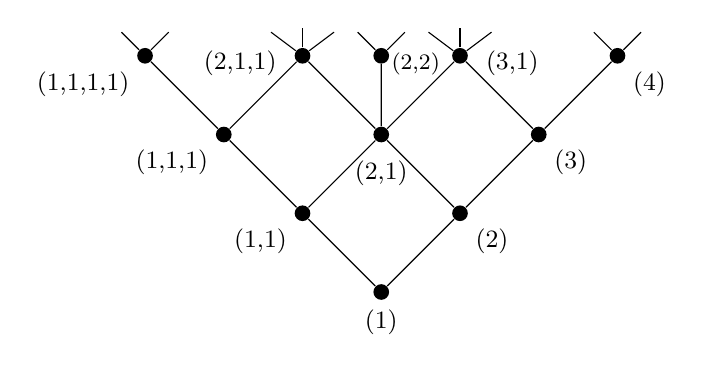
\begin{tikzpicture}[
    dot/.style={circle, fill=black, inner sep=2pt},
    every label/.style={font=\small},
    node distance=12mm and 14mm
]

% level 1 
\node[dot, label=below:{(1)}] (1) at (0,0) {};

% level 2
\node[dot, label=below left:{(1,1)}] (11) at (-1,1) {};
\node[dot, label=below right:{(2)}] (2) at (1,1) {};

% level 3
\node[dot, label=below left:{(1,1,1)}] (111) at (-2,2) {};
\node[dot, label={[yshift=-1mm]below:(2,1)}] (21) at (0,2) {};
\node[dot, label=below right:{(3)}] (3) at (2,2) {};

% level 3
\node[dot, label=below left:{(1,1,1,1)}] (1111) at (-3,3) {};
\node[dot, label={[xshift=-1mm,yshift=-1mm]left:(2,1,1)}] (211) at (-1,3) {};
\node[dot, label={[xshift=-1mm,yshift=-1mm]right:{{\footnotesize(2,2)}}}] (22) at (0,3) {};
\node[dot, label={[xshift=1mm,yshift=-1mm]right:(3,1)}] (31) at (1,3) {};
\node[dot, label=below right:{(4)}] (4) at (3,3) {};

\draw (1)--(11) (1)--(2);
\draw (11)--(111) (11)--(21);
\draw (2)--(21) (2)--(3);
\draw (111)--(1111) (111)--(211);
\draw (21)--(211) (21)--(22) (21)--(31);
\draw (3)--(31) (3)--(4);

% stubs for next level
% (1111) – two stubs
\draw (1111) -- ++(-0.3,0.3);
\draw (1111) -- ++(0.3,0.3);

% (211) – three stubs
\draw (211) -- ++(-0.4,0.3);
\draw (211) -- ++(0,0.35);
\draw (211) -- ++(0.4,0.3);

% (22) – two stubs
\draw (22) -- ++(-0.3,0.3);
\draw (22) -- ++(0.3,0.3);

% (31) – three stubs
\draw (31) -- ++(-0.4,0.3);
\draw (31) -- ++(0,0.35);
\draw (31) -- ++(0.4,0.3);

% (4) – two stubs
\draw (4) -- ++(-0.3,0.3);
\draw (4) -- ++(0.3,0.3);
\end{tikzpicture}
\]

\begin{definition}
    \label{def:poset}
    Το ζεύγος $(P,\leq)$, όπου $P$ είναι σύνολο και $\leq : P\times P \to P$ είναι μια σχέση η οποία είναι 
    \begin{itemize}
        \item \emph{αυτοπαθής}, δηλαδή $x \le x$
        \item \emph{αντισυμμετρική}, δηλαδή αν $x \le y$ και $y \le x$, τότε $x = y$
        \item \emph{μεταβατική}, δηλαδή αν $x \le y$ και $y \le z$, τότε $x \leq z$
    \end{itemize}
    για κάθε $x, y, z \in P$ ονομάζεται \defn{μερική διάταξη} (poset\footnote{Συντομογραφία του {\bf p}artially {\bf o}rdered {\bf set}.}).
\end{definition}

Ένα ακόμα παράδειγμα μερικής διάταξης είναι το ζεύγος $(2^{[n]},\subseteq)$, όπου $2^{[n]}$ είναι το σύνολο όλων των υποσυνόλων του $[n]$, η οποία ονομάζεται \defn{διάταξη Boole}. Για παράδειγμα, 
\[
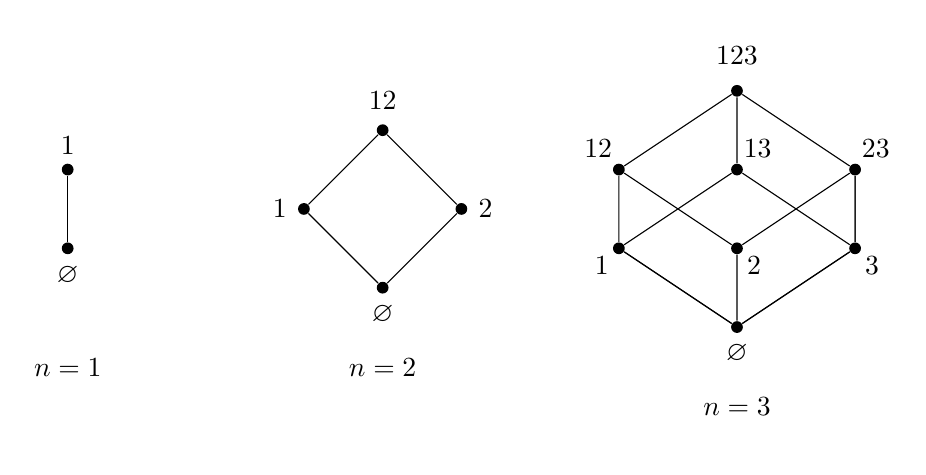
\begin{tikzpicture}[every node/.style={circle, fill, inner sep=1.5pt}]
    \begin{scope}[shift={(0,0.5)}]
    
    \node[label=above:{$1$}] (b) at (0,.5) {};
    \node[label=below:{$\emptyset$}] (a) at (0,-0.5) {};
    \node[below=0.5cm,fill=none] at (0,-1) {$n=1$};

    \draw (a) -- (b);
    \end{scope}

    \begin{scope}[shift={(3,.5)}] 
    \node[label=above:{$12$}] (12) at (1,1) {};
    \node[label=left:{$1$}] (1) at (0,0) {};
    \node[label=right:{$2$}] (2) at (2,0) {};
    \node[label=below:{$\emptyset$}] (0) at (1,-1) {};
    \node[below=0.5cm,fill=none] at (1,-1) {$n=2$};

    \draw (12) -- (1);
    \draw (12) -- (2);
    \draw (1) -- (0);
    \draw (2) -- (0);
    \end{scope}

    \begin{scope}[shift={(7,0)}] 
        \node[label=below left:{$1$}] (a1) at (0,0) {};
        \node[label=below right:{$2$}] (b1) at (1.5,0) {};
        \node[label=below right:{$3$}] (c1) at (3,0) {};
        \node[label=above left:{$12$}] (ab1) at (0,1) {};
        \node[label=above right:{$13$}] (ac1) at (1.5,1) {};
        \node[label=above right:{$23$}] (bc1) at (3,1) {};
        \node[label=above:{$123$}] (abc1) at (1.5,2) {};
        \node[label=below:{$\emptyset$}] (ee1) at (1.5,-1) {};
        \node[below=0.5cm,fill=none] at (1.5,-1) {$n=3$};

        \draw (abc1) -- (ab1) -- (a1) -- (ee1);
        \draw (abc1) -- (bc1) -- (c1) -- (ee1);
        \draw (abc1) -- (ac1) -- (a1) -- (ee1);
        \draw (ab1) -- (b1) -- (ee1);
        \draw (ac1) -- (c1);
        \draw (bc1) -- (b1);
        \draw (bc1) -- (c1) -- (ee1);
    \end{scope}
\end{tikzpicture}
\]

\begin{definition}
    \label{def:composition}
    Μια ακολουθία $\alpha = (\alpha_1, \alpha_2, \dots, \alpha_k)$ θετικών (αντ. μη αρνητικών) ακεραίων τέτοια ώστε 
    \[
    \alpha_1 + \alpha_2 + \cdots + \alpha_k = n
    \]
    ονομάζεται \defn{σύνθεση} (αντ. \defn{ασθενής σύνθεση}) (composition και weak composition, αντίστοιχα) του $n$. Συμβολίζουμε με $\Comp(n)$ το σύνολο όλων των συνθέσεων του $n$.
\end{definition}

Για παράδειγμα, οι συνθέσεις του $n=3$ είναι 
\[
(1,1,1), \quad (1,2), \quad (2,1), \quad \text{και} \quad (3).
\]
Σε αντίθεση με τις διαμερίσεις, το πλήθος των συνθέσεων υπολογίζεται αρκετά εύκολα.
\begin{proposition}
    \label{prop:comp_to_set}
    Η απεικόνιση $\rmset: \Comp(n) \to 2^{[n-1]}$ που ορίζεται θέτοντας 
    \[
    \rmset(\alpha) \coloneqq \{\alpha_1, \alpha_1 + \alpha_2, \dots, \alpha_1 + \cdots + \alpha_{k-1}\}
    \]
    για κάθε $\alpha = (\alpha_1, \alpha_2, \dots, \alpha_k) \in \Comp(n)$ είναι αμφιμονοσήμαντη. Ειδικότερα, 
    \[
    \abs{\Comp(n)} = 2^{n-1}.
    \]
\end{proposition}
\begin{proof}[Απόδειξη]
    Θεωρούμε την απεικόνιση $\comp: 2^{[n-1]} \to \Comp(n)$ που ορίζεται θέτοντας 
    \[
    \comp(S) \coloneqq \left(s_1, s_2-s_1, \dots, s_{k}-s_{k-1}, n-s_k\right)
    \]
    όπου $S = \{s_1, s_2, \dots, s_k\} \subseteq [n-1]$ έτσι ώστε $s_1 < s_2 < \cdots < s_k$. Για παράδειγμα, 
    \[
    \renewcommand{\arraystretch}{1.2}
    \begin{array}{c|c|c|c|c|c|c|c|c}
        S        & \emptyset & 1     & 2     & 3     & 12         & 13      & 23      & 123 \\\hline
        \comp(S) & (4)       & (1,3) & (2,2) & (3,1) & 
        (1,1,2)    & (1,2,1) & (2,1,1) & (1,1,1,1)
    \end{array}
    \]
    Η απεικόνιση $\comp$ είναι η αντίστροφη της $\rmset$ (γιατί;) και το ζητούμενο έπεται.
\end{proof}

\section{Πρότυπα Young}
\label{sec:young_module}

Στο Πόρισμα \ref{cor:irreducible_characters_partitions} είδαμε ότι το σύνολο των ανάγωγων χαρακτήρων της $\fS_n$ παραμετρικοποι\-είται από τις διαμερίσεις του $n$. Στόχος μας στις επόμενες παραγράφους είναι δοθείσης μια διαμέρισης $\lambda \vdash n$, να κατασκευάσουμε ένα ανάγωγο $\fS_n$-πρότυπο $\sS^\lambda$, έτσι ώστε το 
\[
\{\sS^\lambda : \lambda \vdash n\}
\]
να αποτελεί ένα σύνολο ανά δύο μη ισόμορφων ανάγωγων $\fS_n$-προτύπων.

Παρόλο που δεν υπάρχει κάποιος προφανής τρόπος να γίνει αυτό, μπορούμε, ξεκινώντας από μια διαμέριση $\lambda$ της $n$, να κατασκευάσουμε μια υποομάδα $\fS_{\lambda}$ που της αντιστοιχεί με \textquote{φυσικό} τρόπο και να μελετήσουμε τα πρότυπα της μορφής 
\[
V^\triv\!\uparrow_{\fS_\lambda}^{\fS_n},
\]
όπου $V^\triv$ είναι το τετριμμένο $\fS_\lambda$-πρότυπο.

\begin{definition}
    \label{def:young_subgroup}
    Έστω $\lambda = (\lambda_1, \lambda_2, \dots, \lambda_k) \vdash n$. Το σύνολο $\fS_\lambda$ όλων των μεταθέσεων της $\fS_n$ που σταθεροποιούν\footnote{Μια μετάθεση $\pi \in \fS_n$ \defn{σταθεροποιεί} το $S \subseteq [n]$ αν $\pi(S) = S$.} τα σύνολα
    \[
    [\lambda_1 + \cdots + \lambda_{i-1}+1, \lambda_1 + \cdots + + \lambda_{i-1} + \lambda_i]
    \]
    για κάθε $1 \le i \le k$, όπου $\lambda_0 \coloneqq 0$ και $[a,b] \coloneqq \{a, a+1, \dots, b\}$ για $a \leq b$ ονομάζεται \defn{υποομάδα Young} που αντιστοιχεί στην $\lambda$.
\end{definition}

Με άλλα λόγια, ένα στοιχείο της $\fS_\lambda$ μεταθέτει μεταξύ τους τους πρώτους $\lambda_1$ αριθμούς, τους επόμενους $\lambda_2$ αριθμούς κ.ο.κ. Για παράδειγμα, αν $n= 5$ και $\lambda = (2,2,1)$, τότε η $\fS_\lambda$ περιέχει όλες τις μεταθέσεις της $\fS_5$ οι οποίες σταθεροποιούν τα σύνολα 
\[
\{1,2\}, \ \{3,4\}, \ \{5\},
\]
και γι αυτό 
\[
\fS_{(2,2,1)} = \{\epsilon, \, \cycle{1,2}, \, \cycle{3,4}, \, \cycle{1,2}\cycle{3,4}\}.
\]

\begin{remark}
    Αν $G$ και $H$ είναι δύο ομάδες, τότε το $G \times H$ έχει και αυτό δομή ομάδας θέτοντας 
    \[
    (g,h) \ast (g', h') \coloneqq (gg', hh')
    \]
    για κάθε $g, g' \in G$ και $h, h' \in H$. Η τάξη της ομάδας αυτής ισούται με $\abs{G}\abs{H}$. Ομοίως, αν έχουμε ένα αυθαίρετο (πεπερασμένο) πλήθος ομάδων και θεωρήσουμε το καρτεσιανό τους γινόμενο.
\end{remark}

Με την παρατήρηση αυτή κατά νου, η υποομάδα Young είναι όντως υποομάδα της $\fS_n$, διότι 
\begin{align*}
    \fS_\lambda 
    &\cong \fS([\lambda_1]) \times \fS([\lambda_1+1,\lambda_1+\lambda_2]) \times \cdots \times \fS([\lambda_1 + \cdots + \lambda_{k-1}+1, n]) \\
    &\cong \fS_{\lambda_1} \times \fS_{\lambda_2} \times \cdots \times \fS_{\lambda_k},
\end{align*}
όπου ο δεύτερος ισομορφισμός έπεται από το γεγονός ότι $\fS(S) \cong \fS(T)$ αν και μόνο αν $\abs{S} = \abs{T}$ (γιατί;). Στο τρέχον παράδειγμα,  
\begin{align*}
\fS([1,2]) \times \fS([3,4]) \times \fS([5,5]) 
&= \{12, 21\} \times \{34, 43\} \times \{5\} \\
&= \{(12,34,5), (21,34,5), (12, 43, 5), (21, 43, 5)\} \\
&\cong \{12345, 21345, 12435, 21435\} \\
&= \{\epsilon, \cycle{1,2}, \cycle{3,4}, \cycle{12}\cycle{3,4}\} \\
&= \fS_{(2,2,1)}.
\end{align*}

Όπως θα δούμε παρακάτω, το πρότυπο
\[
V^\triv\!\uparrow_{\fS_\lambda}^{\fS_n}
\]
έχει μια αρκετά απλή μορφή ως αναπαράσταση μεταθέσεων για μια δράση της συμμετρικής ομάδας στα εξής συνδυαστικά αντικείμενα.

\begin{definition}
    \label{def:young_tableau}
    \defn{Young ταμπλώ} (Young tableau), ή απλούστερα ταμπλώ, σχήματος $\lambda \vdash n$ και περιεχομένου $[n]$ ονομάζεται μια αμφιμονοσήμαντη αντιστοιχία μεταξύ του συνόλου των τετραγώνων του διαγράμματος Young της $\lambda$ και του $[n]$.
\end{definition}

Για παράδειγμα, ένα ταμπλώ σχήματος $(4,2,2,1)$ και περιεχομένου $[9]$ είναι 
\[
T = \
\begin{ytableau}
7 & 3 & 8 & 2 \\
1 & 5 \\
4 & 9 \\
6
\end{ytableau}.
\]
Τα ταμπλώ σχήματος $(2,1)$ είναι 
\[
\left\{\,
\begin{ytableau}
    1 & 2 \\
    3
\end{ytableau}\,, \
\begin{ytableau}
    2 & 1 \\
    3
\end{ytableau}\,, \
\begin{ytableau}
    1 & 3 \\
    2
\end{ytableau}\,, \
\begin{ytableau}
    3 & 1 \\
    2
\end{ytableau}\,, \
\begin{ytableau}
    2 & 3 \\
    1
\end{ytableau}\,, \
\begin{ytableau}
    3 & 2 \\
    1
\end{ytableau}\,
\right\}.
\]

Η δράση καθορισμού της $\fS_n$ στο $[n]$ επάγει μια δράση στο σύνολο όλων των ταμπλώ σχήματος $\lambda$ και περιεχομένου $[n]$ με τον προφανή τρόπο. Για παράδειγμα, αν $n=9$, $\lambda = (4,2,2,1)$ και $\pi = \cycle{1,3,9,8}\cycle{2,7,6,5,4} \in \fS_9$, τότε 
\[
\pi T = 
\begin{ytableau}
    6 & 9 & 1 & 7 \\
    3 & 4 \\
    2 & 8 \\
    6
\end{ytableau}\, .
\]

Δοθέντος ενός ταμπλώ $T$, θεωρούμε τις υποομάδες $\rmR(T)$ και $\rmC(T)$ της $\fS_n$ που περιέχουν τις μεταθέσεις που σταθεροποιούν τα στοιχεία των γραμμών και των στηλών του $T$, αντίστοιχα. Στο τρέχον παράδειγμα, 
\begin{align*}
    \rmR(T) 
    &\cong \fS(\{2,3,7,8\}) \times \fS(\{1,5\}) \times \fS(\{4,9\}) \times \fS(\{6\}) \\  
    \rmC(T) 
    &\cong \fS(\{1,4,6,7\}) \times \fS(\{3,5,9\}) \times \fS(\{8\}) \times \fS(\{2\}).\\  
\end{align*}

\begin{definition}
    \label{def:young_tabloid}
    Έστω $T$ ένα ταμπλώ σχήματος $\lambda$. Η τροχιά του $T$ στη δράση της $\rmR(T)$ ονομάζεται \defn{ταμπλοειδές} (tabloid) σχήματος $\lambda$ και συμβολίζεται με $[T]$.
\end{definition}

Με άλλα λόγια, η $[T]$ είναι η κλάση ισοδυναμίας με αντιπρόσωπο το ταμπλώ $T$, όπου δύο ταμπλώ ίδιου σχήματος θεωρούνται ισοδύναμα αν και μόνο αν σε κάθε γραμμή έχουν το ίδιο σύνολο στοιχείων. Για παράδειγμα, υπάρχουν τρία ταμπλοειδή σχήματος $(2,1)$ 
\begin{align*}
    \ytableausetup{tabloids}
    \begin{ytableau}
        1 & 2 \\
        3
    \end{ytableau} \ &= 
    \ytableausetup{notabloids}
    \left\{\,
    \begin{ytableau}
    1 & 2 \\
    3
    \end{ytableau}\,, \
    \begin{ytableau}
    2 & 1 \\
    3
    \end{ytableau}\,
    \right\}
    \\[6pt]
    \ytableausetup{tabloids}
    \begin{ytableau}
        1 & 3 \\
        2
    \end{ytableau} \ &= 
    \ytableausetup{notabloids}
    \left\{\,
    \begin{ytableau}
    1 & 3 \\
    2
    \end{ytableau}\,, \
    \begin{ytableau}
    3 & 1 \\
    2
    \end{ytableau}\,
    \right\}
\\[6pt]
\ytableausetup{tabloids}
    \begin{ytableau}
        2 & 3 \\
        3
    \end{ytableau} \ &= 
    \ytableausetup{notabloids}
    \left\{\,
    \begin{ytableau}
    2 & 3 \\
    1
    \end{ytableau}\,, \
    \begin{ytableau}
    3 & 2 \\
    1
    \end{ytableau}\,
    \right\}.
\end{align*}
Στην πράξη, όταν γράφουμε ένα ταμπλοειδές θα \textquote{ξεχνάμε} τις κάθετες γραμμές στο διάγραμμα Young για να υποδείξουμε ότι μπορούμε ελεύθερα να μεταθέσουμε τα στοιχεία κάθε γραμμής και να προκύψει το ίδιο ταμπλοειδές.

Η παραπάνω δράση της $\fS_n$ στα ταμπλώ περιεχομένου $[n]$ επεκτείνεται και στο σύνολο των ταμπλοειδών περιεχομένου $[n]$ θέτοντας 
\[
\pi \cdot [T] \coloneqq [\pi T]
\]
για κάθε $\pi \in \fS_n$ και κάθε ταμπλώ $T$ περιεχομένου $[n]$. 

Η δράση αυτή είναι καλά ορισμένη. Πράγματι, αν $[T] = [Q]$, τότε, από τον Ορισμό~\ref{def:young_tabloid}, $Q = \pi{T}$ για κάποια $\pi \in \rmR(T)$. Συνεπώς, για κάθε $\sigma \in \fS_n$ έχουμε 
\[
\sigma{Q} = \sigma\pi{T} = (\sigma\pi\sigma^{-1})\sigma{T},
\]
όπου $\sigma\pi\sigma^{-1}\in \rmR(\sigma{T})$ (γιατί;\footnote{Για την ακρίβεια, παρατηρήστε ότι $\rmR(\sigma{T}) = \sigma\rmR(T)\sigma^{-1}$ για κάθε $\sigma \in \fS_n$ και κάθε ταμπλώ $T$ περιεχομένου $[n]$.}) και γι αυτό, πάλι από τον Ορισμό~\ref{def:young_tabloid}, $[\sigma{T}] = [\sigma{Q}]$ ή ισοδύναμα $\sigma\cdot[T] = \sigma\cdot[Q]$, όπως θέλαμε.

\begin{definition}
    \label{def:young_module}
    Η αναπαράσταση μεταθέσεων που επάγεται από τη δράση της $\fS_n$ στο σύνολο όλων των ταμπλοειδών σχήματος $\lambda$ ονομάζεται \defn{πρότυπο Young} (Young module) και συμβολίζεται με $\rmM^\lambda$.
\end{definition}

Ας υπολογίσουμε τον χαρακτήρα $\varphi^{(2,1)}$ του προτύπου Young 
\[
\rmM^{(2,1)} = 
\CC\left[\,
    \ytableausetup{tabloids,centertableaux,smalltableaux}
    \begin{ytableau}
        1 & 2 \\
        3
    \end{ytableau} \, , \ 
    \begin{ytableau}
        1 & 3 \\
        2
    \end{ytableau}\, , \ 
    \begin{ytableau}
        2 & 3 \\
        3
    \end{ytableau}
\right]
\]
που αντιστοιχεί στην διαμέριση $\lambda = (2,1)$ του $n=3$. Έχουμε
\[
    \renewcommand{\arraystretch}{2} 
    \begin{array}{c|c|c|c|}
                        & \rmK_{111}      & \rmK_{21}       & \rmK_{3}              \\ \hline
    \text{αντιπρόσωπος} & \epsilon         & \cycle{1,2}      & \cycle{1,2,3} \\ \hline
    \begin{ytableau}
        1 & 2 \\
        3
    \end{ytableau}      & \tcbo{\begin{ytableau}
        1 & 2 \\
        3
    \end{ytableau}} & \tcbo{\begin{ytableau}
        1 & 2 \\
        3
    \end{ytableau}} & \begin{ytableau}
        2 & 3 \\
        3
    \end{ytableau}       \\ \hline 
    \begin{ytableau}
        1 & 3 \\
        2
    \end{ytableau}           & \tcbo{\begin{ytableau}
        1 & 3 \\
        2
    \end{ytableau}} & \begin{ytableau}
        2 & 3 \\
        3
    \end{ytableau}        & \begin{ytableau}
        1 & 2 \\
        3
    \end{ytableau}      \\ \hline 
    \begin{ytableau}
        2 & 3 \\
        3
    \end{ytableau}           & \tcbo{\begin{ytableau}
        2 & 3 \\
        3
    \end{ytableau}} & \begin{ytableau}
        1 & 3 \\
        2
    \end{ytableau}        & \begin{ytableau}
        1 & 3 \\
        2
    \end{ytableau}     \\ \hline 
    \varphi^{(2,1)}                & 3                & 1                & 0                       
    \end{array}\ .
    \]
Τι σας θυμίζει;

\begin{proposition}
    \label{prop:young_module}
    Για κάθε $\lambda \vdash n$, 
    \begin{equation}
        \label{eq:young_module}
        \rmM^\lambda \ \cong_{\fS_n} \ V^\triv\!\uparrow_{\fS_{\lambda}}^{\fS_n}.
    \end{equation}
    Ειδικότερα, 
    \[
    \dim(\rmM^\lambda) = \frac{n!}{\lambda_1!\lambda_2!\cdots\lambda_{\ell(\lambda)}!}.
    \]
\end{proposition}

\begin{proof}[Απόδειξη]
    Ο δεύτερος ισχυρισμός έπεται άμεσα απαριθμώντας το πλήθος των ταμπλοειδών σχήματος $\lambda$ (γιατί;). Εναλλακτικά, υπολογίζοντας τις διαστάσεις και στα δύο μέλη της Ταυτότητας \eqref{eq:young_module}, έπεται ότι 
    \begin{align*}
    \dim(\rmM^\lambda) &= 
    \dim\left(
        V^\triv\!\uparrow_{\fS_{\lambda}}^{\fS_n}
    \right) \\
    &= \chi^\triv\!\uparrow_{\fS_{\lambda}}^{\fS_n}(\epsilon) \\
    &= \frac{\abs{\{\pi \in \fS_n : \pi^{-1}\epsilon\pi \in \fS_n\}}}{\abs{\fS_\lambda}} \\ 
    &= \frac{n!}{\lambda_1!\lambda_2!\cdots\lambda_{\ell(\lambda)}!},
    \end{align*}
    όπου η τρίτη ισότητα έπεται από το Πόρισμα \ref{cor:induction_trivial}. 

    Για τον πρώτο ισχυρισμό, αρκεί να δείξουμε ότι το $\rmM^\lambda$ είναι ισόμορφο με την αναπαράσταση συμπλόκου της $\fS_\lambda$ στην $\fS_n$ (γιατί;). Πράγματι, θεωρούμε την αντιστοιχία που στέλνει το σύμπλοκο $\epsilon\fS_\lambda$ στο \textquote{σύνηθες} ταμπλοειδές
    \[
    \ytableausetup{nosmalltableaux}
    \ytableausetup{boxsize=2em} 
    [T] \ = \ \begin{ytableau}
    1                                                                &&& 2                         &&              & \cdots &&&& \lambda_1 \\
    \scriptstyle \lambda_1 + 1                                       &&& \scriptstyle\lambda_1 + 2 &&  & \cdots &&& \scriptstyle \lambda_1 + \lambda_2 \\
    \vdots                                                           &&& \vdots && &  &  \\
     &\scriptstyle \lambda_1 + \cdots + \lambda_{\ell(\lambda)-1} + 1&               &&\scriptstyle \lambda_1 + \cdots + \lambda_{\ell(\lambda)-1} + 2  &             &
    \cdots &
    n
    \end{ytableau} 
    \]
    και κατά συνέπεια το σύμπλοκο $\pi\fS_n$ στο ταμπλοειδές $\pi[T]$. Η αντιστοιχία αυτή είναι καλά ορισμένη. Πράγματι, αν $\pi\fS_\lambda = \sigma\fS_\lambda$, τότε $\pi = \sigma\tau$ για κάποια $\tau \in \fS_\lambda$ ή ισοδύναμα για κάποια $\tau \in \rmR(T)$. Όμως, 
    \[
    \pi = \left(\sigma\tau\sigma^{-1}\right) \sigma
    \]
    όπου $\sigma\tau\sigma^{-1} \in \rmR(\sigma T)$. Συνεπώς, $\pi = w\sigma$, για κάποια $w \in \rmR(\sigma T)$ και γι αυτό $\pi[T] = \sigma[T]$, όπως θέλαμε. Επεκτείνοντας γραμμικά προκύπτει ο ζητούμενος $\fS_n$-ισομορφισμός (γιατί;).
\end{proof}

\section{Πρότυπα Specht}
\label{sec:specht_modules}

Όπως είδαμε στο τέλος της προηγούμενης παραγράφου, τα πρότυπα Young δεν είναι ανάγωγα για κάθε διαμέριση $\lambda$. Πιο συγκεκριμένα, αν $\lambda = (n)$, τότε 
\[
\ytableausetup{smalltableaux}
\rmM^{(n)} = \CC\left[\ \begin{ytableau}
        1 & 2 & \cdots & n 
    \end{ytableau} \ \right]
\]
είναι το τετριμμένο $\fS_n$-πρότυπο. Αυτή είναι και η μόνη περίπτωση όπου το $\rmM^\lambda$ είναι ανάγωγο. 

Αν $\lambda = (1^n)$ είναι η διαμέριση με $n$ μέρη ίσα με 1, τότε υπάρχουν $n!$ το πλήθος ταμπλοειδή σχήματος $(1^n)$ και κάθε τέτοιο αντιστοιχεί σε μια μετάθεση της $\fS_n$ ως εξής 
\[
\ytableausetup{nosmalltableaux}
\begin{ytableau}
    \pi_1 \\
    \pi_2 \\
    \vdots \\
    \pi_n 
\end{ytableau} \ \mapsto \ \pi_1\pi_2\cdots\pi_n.
\]
Συνεπώς, το $\rmM^{(1^n)}$ δεν είναι άλλο από το πρότυπο της κανονικής αναπαράστασης της $\fS_n$ (γιατί;).

Τέλος, αν $\lambda = (n-1,1)$, τότε υπάρχουν $n$ το πλήθος ταμπλοειδή σχήματος $(n-1,1)$ και κάθε ένα από αυτά αντιστοιχεί σε ένα στοιχείο του $[n]$ ως εξής 
\[
\begin{ytableau}
    \ast & \ast & \cdots & \ast\\ 
    i
\end{ytableau} \ \mapsto \ i.
\]
Συνεπώς, το $\rmM^{(n-1,1)}$ δεν είναι άλλο από το πρότυπο της αναπαράστασης καθορισμού της $\fS_n$ (γιατί;).

Επιστρέφοντας στον στόχο μας, δηλαδή να κατασκευάσουμε ένα ανάγωγο $\fS_n$-πρότυπο $\sS^\lambda$, για κάθε $\lambda \vdash n$, συνδυάζοντας τους παραπάνω υπολογισμούς με αυτά που έχουμε δει σε προηγούμενες παραγράφους βρίσκουμε
%
\begin{align*}
    \rmM^{(3)}   &\cong \sS^{(3)} \\ 
    \rmM^{(2,1)} &\cong \sS^{(3)} \oplus \sS^{(2,1)} \\ 
    \rmM^{(1,1,1)} &\cong \sS^{(3)} \oplus \left(\sS^{(2,1)}\right)^2 \oplus \sS^{(1,1,1)},
\end{align*}
%
όπου με $\sS^{(3)}, \sS^{(2,1)}$ και $\sS^{(1,1,1)}$ συμβολίσαμε τα πρότυπα της τετριμμένης, της συνήθους και της αναπαράστασης προσήμου, αντίστοιχα.

Η παρατήρηση αυτή γεννάει την εξής ιδέα: Να βρούμε μια ολική διάταξη\footnote{\emph{Ολική διάταξη} ονομάζεται μια μερική διάταξη $(P,\le)$ όπου για κάθε δύο στοιχεία $x, y \in P$ ισχύει ότι $x < y$ ή $y < x$.} 
\[
\lambda^{(1)} > \lambda^{(2)} > \cdots >\lambda^{(\rmp(n))}
\]
στο σύνολο $\Par(n)$ των διαμερίσων του $n$ τέτοια ώστε το $\rmM^{\lambda^{(1)}}$ να είναι ανάγωγο, έστω $\sS^{\lambda^{(1)}}$, το $\rmM^{\lambda^{(2)}}$ να αποτελείται από κάποια αντίγραφα του $\sS^{\lambda^{(1)}}$ και \emph{ακριβώς} ένα αντίγραφο ενός νέου ανάγωγου προτύπου, έστω $\sS^{\lambda^{(2)}}$ κ.ο.κ. μέχρι να εξαντλήσουμε όλες τις διαμερίσεις του $n$. Για $n=3$, η ζητούμενη ολική διάταξη είναι 
\[
(3) > (2,1) > (1,1,1).
\]

Προς αυτή την κατεύθυνση, θα εξερευνήσουμε τις συμμετρίες των Young ταμπλώ.

\begin{definition}
    \label{def:anti-symmetrizer}
    Έστω $T$ ταμπλώ σχήματος $\lambda \vdash n$. Τα στοιχεία\footnote{Ο συμβολισμός δεν είναι στάνταρ στην βιβλιογραφία.}
    \begin{align*}
        \nabla_T^+ &\coloneqq \sum_{\pi \in \rmR(T)} \pi \\
        \nabla_T^- &\coloneqq \sum_{\pi \in \rmC(T)} \sign(\pi)\pi \\
    \end{align*}
    του $\CC[\fS_n]$ ονομάζονται \defn{συμμετρικοποιητής γραμμών} (row symmetrizer) και \defn{αντισυμμετρικοποιητής στηλών} (column antisymmetrizer) του $T$, αντίστοιχα.
\end{definition}

Για παράδειγμα, αν
\[
\ytableausetup{notabloids}
T = \
\begin{ytableau}
    3 & 1 & 4 \\
    5 & 2 
\end{ytableau}
\]
τότε 
\begin{align*}
    \rmR(T) &= \fS(\{1,3,4\})\times\fS(\{2,5\}) \\
    \rmC(T) &= \fS(\{3,5\})\times\fS(\{1,2\})\times\fS(\{4\}) \\
\end{align*}
και γι αυτό 
\begin{align*}
\nabla_T^+ &= (\epsilon + \cycle{1,3} + \cycle{3,4} + \cycle{1,3,4} + \cycle{1,4,3})(\epsilon  + \cycle{2,5}) \\
\nabla_T^- &= \epsilon -\cycle{3,5} - \cycle{1,2} + \cycle{3,5}\cycle{1,2}.
\end{align*}

\begin{definition}
    \label{def:polytabloid}
    Έστω $T$ ένα ταμπλώ σχήματος $\lambda \vdash n$. Το  
    \[
    \bfe_T \coloneqq \nabla_T^- [T] \ \in \ \rmM^\lambda
    \]
    ονομάζεται \defn{πολυταμπλοειδές} (polytabloid) και ο υπόχωρος $\sS^\lambda$ που παράγεται από όλα τα $\bfe_T$, καθώς το $T$ διατρέχει τα ταμπλώ σχήματος $\lambda$ ονομάζεται \defn{πρότυπο Specht} (Specht module).
\end{definition}

Κάθε ταμπλοειδές είναι ουσιαστικά γραμμικός συνδυασμός (με συντελεστές στο $\ZZ$) ταμπλοειδών εντός του αντίστοιχου προτύπου Young. Στο παράδειγμα, 
\begin{align*}
    \ytableausetup{smalltableaux,notabloids}
    \bfe_{\ytableaushort{314, 52}} 
    \ytableausetup{smalltableaux,tabloids} 
    &= \left(\epsilon -\cycle{3,5} - \cycle{1,2} + \cycle{3,5}\cycle{1,2}\right)\ytableaushort{314, 52} \\
    &= \ytableaushort{314, 52} \ - \ \ytableaushort{514, 32} \ - \ \ytableaushort{324, 51} \ + \ \ytableaushort{524, 31} \\
    &= \ytableaushort{134, 25} \ - \ \ytableaushort{145, 23} \ - \ \ytableaushort{234, 15} \ + \ \ytableaushort{245, 13} \ \in \rmM^{(3,2)}.
\end{align*}
Παρατηρήστε ότι ένα πολυταμπλοειδές εξαρτάται από το ταμπλώ $T$ και όχι από το ταμπλοειδές $[T]$ με αντιπρόσωπο $T$. Ποιό είναι, για παράδειγμα, το πολυταμπλοειδές 
\[
\ytableausetup{smalltableaux,notabloids}
\bfe_{\ytableaushort{134, 52}}\, ;
\]
Επίσης, από τον Ορισμό~\ref{def:polytabloid}, δεν έπεται άμεσα ότι το πρότυπο Specht είναι όντως $\fS_n$-πρότυπο.


\begin{example}
    \label{ex:specht_modules}
    \leavevmode
    \begin{itemize}
        \item[(1)] Έστω $\lambda = (2,1) \vdash 3$. Για κάθε ένα από τα έξι ταμπλώ σχήματος $\lambda$
        \[
        \ytableausetup{nosmalltableaux}
        \begin{ytableau}
            1 & 2 \\
            3
        \end{ytableau}\,, \quad
        \begin{ytableau}
            2 & 1 \\
            3
        \end{ytableau}\,, \quad
        \begin{ytableau}
            1 & 3 \\
            2
        \end{ytableau}\,, \quad
        \begin{ytableau}
            3 & 1 \\
            2
        \end{ytableau}\,, \quad
        \begin{ytableau}
            2 & 3 \\
            1
        \end{ytableau}\,, \quad
        \begin{ytableau}
            3 & 2 \\
            1
        \end{ytableau}
        \]
        παίρνουμε ένα πολυταμπλοειδές. Για διαφορετικούς αριθμούς $a, b, c \in [3]$, έχουμε
        \[
        \ytableausetup{smalltableaux,notabloids}
        \bfe_{\ytableaushort{ab, c}} \ = \ 
        \nabla_{\ytableaushort{ab, c}}^- \
        \ytableausetup{smalltableaux,tabloids}
        \ytableaushort{ab, c} \ = \
        \left(\epsilon - \cycle{a,c}\right) \ \ytableaushort{ab, c}   \ = \
        \ytableaushort{ab, c} \ - \ \ytableaushort{cb, a}\ .
        \]
        Χρησιμοποιώντας τον ισομορφισμό $\rmM^{(2,1)} \cong \CC[1,2,3]$ που είδαμε στην αρχή της παραγράφου, προκύπτει ότι 
        \[
        \ytableausetup{smalltableaux,notabloids}
        \bfe_{\ytableaushort{ab, c}} \ \mapsto c - a. 
        \]
        Με άλλα λόγια, το πρότυπο Specht $\sS^{(2,1)}$ παράγεται από όλες τις διαφορές $c - a$ για κάθε $c \neq a$ στο $\rmM^{(2,1)}$. Όπως είδαμε στο Παράδειγμα \ref{ex:standard_representation}, αυτό δεν είναι άλλο από την συνήθη αναπαράσταση της $\fS_3$ και γι αυτό
        \[
        \sS^{(2,1)} = \CC[\,\bfe_{\ytableaushort{12, 3}}\, , \bfe_{\ytableaushort{13, 2}} \ ].
        \]
        Γενικότερα, το $\sS^{(n-1,1)}$ είναι ένα ανάγωγο υποπρότυπο του $\rmM^{(n-1,1)}$ ισόμορφο με τη συνήθη αναπαράσταση της $\fS_n$.

        \item[(2)] Αν $\lambda = (n)$, τότε υπάρχει ακριβώς ένα ταμπλώ σχήματος $(n)$ και γι αυτό 
        \[
        \ytableausetup{smalltableaux,notabloids}
        \bfe_{\ytableaushort{12\cdots{n}}} \ = \
        \nabla_{\ytableaushort{12\cdots{n}}}^- \
        \ytableausetup{smalltableaux,tabloids,centertableaux}
        \ytableaushort{12\cdots{n}} \ = \ \ytableaushort{12\cdots{n}} \, .
        \]
        Με άλλα λόγια, $\sS^{(n)} = \rmM^{(n)}$. 

        \item[(3)] Αν $\lambda = (1^n)$, τότε για κάθε ταμπλώ $T$ σχήματος $(1^n)$ έχουμε $\rmC(T) = \fS_n$ (γιατί;) και γι αυτό 
        \[
        \nabla_T^- = \sum_{\pi \in \rmC(T)} \sign(\pi)\pi = \sum_{\pi \in \fS_n} \sign(\pi)\pi \coloneqq \nabla_n^-.
        \]
        Συνεπώς, για ένα αυθαίρετο πολυταμπλοειδές σχήματος $(1^n)$ υπολογίζουμε
        \begin{align*}
            \ytableausetup{smalltableaux,notabloids}
            \ytableausetup{boxsize=1.3em}
            \bfe_{\ytableaushort{{\pi_1},{\pi_2},\vdots,{\pi_n}}} 
            &= \sum_{\sigma \in \fS_n} \sign(\sigma)\sigma \ 
            \ytableausetup{nosmalltableaux,tabloids,centertableaux} 
            \ytableaushort{{\pi_1},{\pi_2},\vdots,{\pi_n}} \\
            &\mapsto \sum_{\sigma \in \fS_n} \sign(\sigma)\sigma\pi \\
            &= \sign(\pi^{-1}) \sum_{\sigma \in \fS_n} \sign(\sigma\pi)\sigma\pi \\
            &= \sign(\pi) \sum_{\tau \in \fS_n} \sign(\tau)\tau \\
            &= \sign(\pi)\nabla_n^-,
        \end{align*}
        όπου στη δεύτερη γραμμή χρησιμοποιήσαμε τον ισομορφισμό $M^{(1^n)} \cong \CC[\fS_n]$ και η δεύτερη και τρίτη ισότητα έπονται από την Άσκηση 3.6 (4). 

        Άρα, το $\sS^{(1^n)}$ είναι ισόμορφο με το υποπρότυπο $\CC[\nabla_n^+]$ της κανονικής αναπαράστασης με τη δράση να δίνεται από το πρόσημο μιας μετάθεσης. Αυτό δεν είναι άλλο από το πρότυπο της αναπαράστασης προσήμου της $\fS_n$.
    \end{itemize}
\end{example}

Οι υπολογισμοί του Παραδείγματος \ref{ex:specht_modules} δείχνουν ότι \textquote{βαδίζουμε} στο σωστό μονοπάτι αναφορικά με τον στόχο μας να βρούμε τα ανάγωγα $\fS_n$-πρότυπα. Η επόμενη πρόταση εξερευνεί ορισμένες ιδιότητες των προτύπων Specht. Η απόδειξη, αν και τεχνική, δεν παρουσιάζει δυσκολίες και είναι μια καλή ευκαιρία να ελέγξει κανείς την κατανόηση των ορισμών.

\begin{lemma}
    \label{lem:specht_module}
    Αν $T$ είναι ταμπλώ περιεχομένου $[n]$ και $\pi \in \fS_n$, τότε ισχύουν τα εξής 
    \begin{itemize}
        \item[(1)] $\rmC(\pi{T}) = \pi\rmC(T)\pi^{-1}$
        \item[(2)] $\nabla_{\pi{T}}^- = \pi\nabla_{T}^-\pi^{-1}$
        \item[(3)] $\bfe_{\pi{T}} = \pi\bfe_T$
        \item[(4)] Αν επιπλεόν $\pi \in \rmC(T)$, τότε $\bfe_{\pi{T}} = \sign(\pi)\bfe_T$.
    \end{itemize}
\end{lemma}

\begin{proof}[Απόδειξη]
    Για το (1), έχουμε $\sigma \in \rmC(\pi{T})$ αν και μόνο αν για κάθε $i \in [n]$, τα $\sigma(i)$ και $i$ βρίσκονται στην ίδια στήλη του $\pi{T}$. Ισοδύναμα, αν και μόνο αν για κάθε $j \in [n]$, τα $\sigma(\pi(j))$ και $\pi(j)$ βρίσκονται στην ίδια στήλη του $\pi{T}$, καθώς η $\pi$ είναι μετάθεση. Με τη σειρά του, αυτό είναι ισόδυναμο με το να βρίσκονται τα $\pi^{-1}(\sigma(\pi(j)))$ και $j$ στην ίδια στήλη του $T$, για κάθε $j \in [n]$ (γιατί;), δηλαδή με το $\pi^{-1}\sigma\pi \in \rmC(T)$ και γι αυτό $\sigma \in \pi\rmC(T)\pi^{-1}$.

    Για το (2), υπολογίζουμε 
    \begin{align*}
        \pi\nabla_{T}^-\pi^{-1} 
        &= \sum_{\sigma \in \rmC(T)} \sign(\sigma) \pi\sigma\pi^{-1} \\
        &= \sum_{\sigma \in \rmC(T)} \sign(\pi\sigma\pi^{-1}) \pi\sigma\pi^{-1} \\
        &= \sum_{\tau \in \pi\rmC(T)\pi^{-1}} \sign(\tau) \tau \\
        &= \sum_{\tau \in \rmC(\pi{T})} \sign(\tau) \tau \\
        &= \nabla_{\pi{T}}^-,
    \end{align*}
    όπου η προτελευταία ισότητα έπεται από το (1).

    Για το (3), έχουμε 
    \begin{align*} 
        \bfe_{\pi{T}} 
        = \nabla_{\pi{T}}^-[\pi{T}] 
        = \pi\nabla_{T}^-\pi^{-1}[\pi{T}] 
        = \pi\nabla_{T}^-[T] 
        = \pi\bfe_T,
    \end{align*}
    όπου η δεύτερη ισότητα έπεται από το (2).

    Τέλος, για το (4), έχουμε 
    \begin{align*}
        \bfe_{\pi{T}} 
        &= \nabla_{\pi{T}}^-[\pi{T}] \\
        &= \sum_{\sigma \in \rmC(\pi{T})}\sign(\sigma)\sigma[\pi{T}] \\
        &= \sum_{\sigma \in \rmC(T)}\sign(\sigma)\sigma[\pi{T}] \\
        &= \sign(\pi^{-1})\sum_{\sigma \in \rmC(T)}\sign(\sigma\pi)\sigma\pi[T] \\
        &= \sign(\pi)\sum_{\tau \in \rmC(T)}\sign(\tau)\tau[T] \\
        &= \sign(\pi)\nabla_T^-[T] \\
        &= \sign(\pi)\bfe_T,
    \end{align*}
    όπου η τρίτη ισότητα έπεται από το (1) και το γεγονός ότι $\pi \in \rmC(T)$ και η πέμπτη ισότητα έπεται από το ότι η αντιστοιχία $\sigma \mapsto \sigma\pi$ είναι αμφιμονοσήμαντη στο $\rmC(T)$, καθώς $\pi \in \rmC(T)$.
\end{proof}

Μια σημαντική συνέπεια του Λήμματος \ref{lem:specht_module}~(3) είναι ότι το πρότυπο Specht είναι υποπρότυπο του προτύπου Young. Πράγματι, για κάθε $\lambda \vdash n$ αν 
\[
v = \sum_{T} c_T \, \bfe_T \ \in \ \sS^\lambda,
\]
όπου το άθροισμα διατρέχει όλα τα ταμπλώ σχήματος $\lambda$, και $c_T \in \CC$, τότε, 
\[
\pi{v} = \pi\left(\sum_{T} c_T \, \bfe_T\right) = \sum_{T} c_T \, (\pi\bfe_T) = \sum_{T} c_T \, \bfe_{\pi{T}} \ \in \ \sS^\lambda,
\]
για κάθε $\pi \in \fS_n$.

Για την ακρίβεια, μπορούμε να πούμε κάτι παραπάνω. Τα πρότυπα Young και Specht έχουν την ιδιότητα ένα αυθαίρετο στοιχείο τους να έχει την μορφή 
\[
\left(\sum_{\pi \in \fS_n}c_\pi\pi\right)[T]
\quad
\text{και}
\quad
\left(\sum_{\pi \in \fS_n}c_\pi\pi\right)\bfe_T
\]
για οποιοδήποτε ταμπλοειδές $[T]$ και πολυταμπλοειδές $\bfe_T$, αντίστοιχα (γιατί;). Ορισμένες φορές πρότυπα με αυτή την ιδιότητα ονομάζονται \emph{κυκλικά}.

\begin{digression_a}
    Γενικότερα, αν $G$ είναι μια πεπερασμένη ομάδα, τότε η κανονική αναπαράσταση $\FF[G]$, εκτός από δομή διανυσματικού χώρου έχει και τη δομή \emph{δακτύλιου}, με τον πολλαπλασιασμό να κληρονομείται από την πράξη στην $G$. Πιο συγκεκριμένα, 
    \[
    \left(\sum_{g \in G} c_g{g}\right)
    \left(\sum_{x \in G} c_x{x}\right) \ \coloneqq \ 
    \sum_{h \in G} \left(\sum_{\substack{g, x \in G \\ h = gx}}c_gc_x\right){h}.
    \]
    Αυτό ονομάζεται \emph{ομαδοδακτύλιος} (group ring).
    
    Έχοντας αυτό κατά νου, αυτά που ονομάζουμε $G$-πρότυπα μέχρι στιγμής, δεν είναι τίποτα άλλο παρά (αριστερά) $\FF[G]$-πρότυπα. Διαισθητικά, ένα πρότυπο πάνω από έναν δακτύλιο $R$ είσαι σαν ένα \textquote{διανυσματικό χώρο}, μόνο που τώρα ο βαθμωτός πολλαπλασιασμός δίνεται από τα στοιχεία του $R$, αντί για τα στοιχεία κάποιου σώματος $\FF$.
    
    Πιο συγκεκριμένα, ένα (\emph{αριστερό}) \emph{$R$-πρότυπο} (left $R$-module) είναι μια αβελιανή ομάδα $M$ εφοδιασμένη με μια πράξη $R \times M \to M$, την οποία συμβολίζουμε με $(r,m) \mapsto r\cdot{m}$ τέτοια ώστε 
    \begin{align*}
        1\cdot{m} &= m \\
        r\cdot{(m+m')} &= r\cdot{m} + r\cdot{m'} \\
        (r+r')\cdot{m} &= r\cdot{m} + r'\cdot{m} \\
        (rr')\cdot{m} &= r\cdot(r'\cdot(m)) 
    \end{align*}
    για κάθε $r, r' \in R$ και $m, m' \in M$. Συγκρίνοντας αυτά τα αξιώματα με τα αντίστοιχα ενός $G$-προτύπου, τι παρατηρείτε; Ποια είναι τα $\FF$-πρότυπα; Ποιά ειναι τα $\ZZ$-πρότυπα;

    Σε αυτό το πλαίσιο, ένα $R$-πρότυπο $M$ ονομάζεται \emph{κυκλικό} αν $M = Rm$, δηλαδή 
    \[
    M = \{rm : r \in R\}
    \]
    για κάποιο (μη μηδενικό) $m \in M$. Η έννοια του κυκλικού $\FF[G]$-προτύπου δεν είναι ακριβώς ίδια με την παραπάνω που έχουν τα πρότυπα Young και Specht. Ειδικότερα, τα πρότυπα Young παράγονται από οποιοδήποτε ταμπλοειδές, αλλά όχι οποιοδήποτε \emph{γραμμικό συνδυασμό ταμπλειδών}, που είναι και ένα αυθαίρετο στοιχείο του $\rmM^\lambda$. Από την άλλη μεριά όμως, θα δείξουμε ότι τα πρότυπα Specht είναι ανάγωγα και ως τέτοια είναι κυκλικά \emph{και} με τις δύο έννοιες\footnote{Δεν είναι δύσκολο να δείξει κανείς ότι ένα μη-τετριμμένο $\FF[G]$-πρότυπο είναι ανάγωγο αν και μόνο αν είναι κυκλικό ως $\FF[G]$-πρότυπο και παράγεται από κάθε (μη μηδενικό) στοιχείο.}. 
\end{digression_a}

Θα δείξουμε τώρα ότι τα πρότυπα Specht είναι ανάγωγα. Γι αυτό θεωρούμε το (μοναδικό) εσωτερικό γινόμενο $(\Arg, \Arg)$ στο $\rmM^\lambda$ που ορίζεται κάνοντας την βάση των ταμπλοειδών σχήματος $\lambda$ ορθοκανονική, δηλαδή
\[
([T], [Q]) = 
\begin{cases}
    1, &\ \text{αν $[T] = [Q]$} \\
    0, &\ \text{διαφορετικά}. \\
\end{cases}
\]
Το $(\Arg,\Arg)$ είναι $\fS_n$-αναλλοίωτο (γιατί;).

% James 1976
\begin{theorem}{\rm(James' submodule theorem)}
    \label{thm:james}
    Έστω $\lambda \vdash n$. Αν $U$ είναι υποπρότυπο του $\rmM^\lambda$, τότε είτε $U \supseteq \sS^\lambda$, ή $U \subseteq (\sS^\lambda)^\perp$, ως προς το εσωτερικό γινόμενο $(\Arg, \Arg)$.
\end{theorem}

Αυτό έχει ως άμεση συνέπεια το παρακάτω.
\begin{corollary}
    \label{cor:specht_irreducible}
    Τα πρότυπα Specht είναι ανάγωγα.
\end{corollary}
\begin{proof}[Απόδειξη]
    Έστω $\lambda$ μια διαμέριση ακεραίου. Αν $U \neq \{0\}$ είναι υποπρότυπο του $\sS^\lambda$, τότε από το Θεώρημα \ref{thm:james} έπεται ότι 
    \begin{itemize}
    \item είτε $U \supseteq \sS^\lambda$ και γι αυτό $U = \sS^\lambda$,      
    \item ή $U \subseteq (\sS^\lambda)^\perp$ και γι αυτό $U \subseteq \sS^\lambda \cap (\sS^\lambda)^\perp = \{0\}$, το οποίο είναι αδύνατο καθώς $U \neq \{0\}$. 
    \end{itemize}
    Με άλλα λόγια, το $\sS^\lambda$ δεν έχει γνήσια υποπρότυπα διαφορετικά του $\{0\}$ και κατά συνέπεια είναι ανάγωγο.
\end{proof}

Η απόδειξη του Θεωρήματος \ref{thm:james} βασίζεται στο παρακάτω τεχνικό λήμμα.
\begin{lemma}
    \label{lem:james}
    Έστω $\lambda \vdash n$ και $T, Q$ δύο ταμπλώ σχήματος $\lambda$. 
    \begin{itemize}
        \item[(1)] Για κάθε $v, u \in \rmM^\lambda$, ισχύει ότι $(\nabla_T^-v, u) = (v, \nabla_T^-u)$.
        \item[(2)] Αν $\cycle{i,j} \in \rmR(Q) \cap \rmC(T)$, τότε $\nabla_T^-[Q] = 0$.
        \item[(3)] Αν $\nabla_T^-[Q] \neq 0$, τότε $\nabla_T^-[Q] = \pm \bfe_T$.
        \item[(4)] Αν $v \in \rmM^\lambda$, τότε 
        \[
        \nabla_T^-v = c \, \bfe_T
        \]
        για κάποιο $c \in \CC$.
    \end{itemize}
\end{lemma}

\begin{proof}[Απόδειξη]
    Για το (1), υπολογίζουμε 
    \begin{align*}
        (\nabla_T^-v, u) 
        &= \left( \sum_{\pi \in \rmC(T)} \sign(\pi)\pi v, u \right) \\
        &= \sum_{\pi \in \rmC(T)} \sign(\pi)\left(\pi v, u\right) \\
        &= \sum_{\pi \in \rmC(T)} \sign(\pi)\left(v,\pi^{-1}u\right) \\
        &= \left(v,\sum_{\pi \in \rmC(T)} \sign(\pi)\pi^{-1}u\right) \\
        &= \left(v,\sum_{\pi \in \rmC(T)} \sign(\pi^{-1})\pi^{-1}u\right) \\
        &= \left(v,\nabla_T^-u\right),
    \end{align*}
    όπου η τρίτη ισότητα έπεται από το γεγονός ότι το $(\Arg,\Arg)$ είναι $\fS_n$-αναλλοίωτο.

    Για το (2), αρχικά παρατηρούμε ότι 
    \begin{equation}
        \label{eq:james_help}
        \nabla_T^- = x(\epsilon - \cycle{i,j}),
    \end{equation}
    για κάποιο $x \in \CC[\fS_n]$. Πράγματι, έστω $H$ η υποομάδα της $\rmC(T)$ που παράγεται από το $\cycle{i,j}$, το οποίο εξ υποθέσεως είναι στοιχείο της $\rmC(T)$, και $\{x_1, x_2, \dots, x_k\}$ ένα σύνολο αντιπροσώπων των αριστερών κλάσεων της $H$ στην $\rmC(T)$. Τότε 
    \[
    \rmC(T) = x_1H \uplus x_2H \uplus \cdots \uplus x_kH
    \]
    και γι αυτό 
    \begin{align*}
        \nabla_T^- 
        &= \sum_{\pi \in \rmC(T)} \sign(\pi) \pi \\
        &= \sum_{i=r}^k \left(\sign(x_r)x_r + \sign(x_r\cycle{i,j})x_r\cycle{i,j}\right) \\
        &= \left(\underbrace{\sum_{r=1}^k \sign(x_r)x_r}_{= \ x}\right)(\epsilon - \cycle{i,j}).
    \end{align*}
    Τώρα, εφαρμόζοντας της Ταυτότητα~\eqref{eq:james_help} παίρνουμε 
    \[
    \nabla_T^-[Q] 
    = x(\epsilon - \cycle{i,j})[Q]
    = x([Q] - \cycle{i,j}[Q]) 
    = x([Q]- [Q])
    =0,
    \]
    όπου η τρίτη ισότητα έπεται από την υπόθεση $\cycle{i,j} \in \rmR(Q)$.

    Για το (3), παρατηρούμε ότι κάθε δύο στοιχεία $i$ και $j$ τα οποία ανήκουν στην ίδια γραμμή του $Q$ \emph{δεν μπορούν} να ανήκουν στην ίδια στήλη του $T$, διότι διαφορετικά $\cycle{i,j} \in \rmR(Q) \cap \rmC(T)$ και από το (2) θα είχαμε $\nabla_T^-[Q] = 0$, το οποίο είναι αδύνατο. Αυτό έχει ως αποτέλεσμα την ύπαρξη μιας $\pi \in \rmC(T)$ τέτοια ώστε $[\pi{T}] = [Q]$.

    Για παράδειγμα, αν $\lambda = (4,3,3,1)$ και 
    \[
    T = 
    \ytableausetup{nosmalltableaux,notabloids}
    \ytableaushort{1234,567,89{10},{11}}
    \quad 
    \text{και}
    \quad
    Q = \ytableaushort{16{10}4,27{11},389,5}
    \]
    τότε \textquote{κοιτάμε} τα στοιχεία κάθε στήλης του $T$ ξεχωριστά για το αν βρίσκονται στην αντίστοιχη γραμμή του $Q$. Αν όχι, τότε τα μεταθέτουμε με ένα στοιχείο της $\rmC(T)$ για να βρεθούν στην \textquote{σωστή} τους θέση. Στο παράδειγμα, στην πρώτη στήλη έχουμε 
    \[
    T = 
    \begin{ytableau}
        1 & 2 & 3 & 4 \\
        *(burntorange)5 & 6 & 7 \\
        8 & 9 & 10 \\
        *(burntorange)11
    \end{ytableau}
    \quad 
    \text{και}
    \quad
    Q = 
    \begin{ytableau}
        1 & 6 & 10 & 4 \\
        2 & 7 & *(burntorange)11 \\
        3 & 8 & 9 \\
        *(burntorange)5
    \end{ytableau}
    \]
    και γι αυτό δρούμε με την $\cycle{5, 11}$. Έπειτα, για τη δεύτερη στήλη έχουμε
    \[
    \cycle{5, 11}T = 
    \begin{ytableau}
        1  & *(iceberg)2 & 3 & 4 \\
        11 & *(iceberg)6 & 7 \\
        8  & 9 & 10 \\
        5
    \end{ytableau}
    \quad 
    \text{και}
    \quad
    Q = 
    \begin{ytableau}
        1 & *(iceberg)6 & 10 & 4 \\
        *(iceberg)2 & 7 & 11 \\
        3 & 8 & 9 \\
        5
    \end{ytableau}
    \]
    και γι αυτό δρούμε με την $\cycle{2,6}$. Τέλος, για την τρίτη στήλη 
    \[
    \cycle{2,6}\cycle{5, 11}T = 
    \begin{ytableau}
        1  & 6 & *(applegreen)3 & 4 \\
        11 & 2 & 7 \\
        8  & 9 & *(applegreen)10 \\
        5
    \end{ytableau}
    \quad 
    \text{και}
    \quad
    Q = 
    \begin{ytableau}
        1 & 6 & *(applegreen)10 & 4 \\
        2 & 7 & 11 \\
        *(applegreen)3 & 8 & 9 \\
        5
    \end{ytableau}
    \]
    και γι αυτό δρούμε με την $\cycle{3,10}$, για να πάρουμε 
    \[
    [\cycle{3,10}\cycle{2,6}\cycle{5, 11}T] \ = \
    \ytableausetup{tabloids}
    \begin{ytableau}
        1  & 6 & 10 & 4 \\
        11 & 2 & 7 \\
        8  & 9 & 3 \\
        5
    \end{ytableau}
    \ = \
    \begin{ytableau}
        1 & 6 & 10 & 4 \\
        2 & 7 & 11 \\
        3 & 8 & 9 \\
        5
    \end{ytableau}
    = [Q].
    \]

    Συνεπώς, 
    \begin{align*}
        \nabla_T^-[Q] 
        &= \nabla_T^-[\pi{T}] \\
        &= \sum_{\sigma \in \rmC(T)} \sign(\sigma) \sigma\pi[T] \\
        &= \sign(\pi^{-1})\sum_{\sigma \in \rmC(T)} \sign(\sigma\pi) \sigma\pi[T] \\
        &= \sign(\pi)\sum_{\tau \in \rmC(T)} \sign(\tau) \tau[T] \\
        &= \sign(\pi)\bfe_{T},
    \end{align*}
    όπου η τέταρτη ισότητα έπεται από το ότι η αντιστοιχία $\sigma \mapsto \sigma\pi$ είναι αμφιμονοσήμαντη στο $\rmC(T)$, διότι $\pi \in \rmC(T)$.

    Τέλος, για το (4), έστω
    \[
    v = \sum_{[Q]} c_{[Q]}[Q] \ \in \ \rmM^\lambda, \ 
    \]
    όπου στο άθροισμα το $[Q]$ διατρέχει όλα τα ταμπλοειδή σχήματος $\lambda$ και $c_{[Q]} \in \CC$. Υπολογίζουμε
    \begin{align*}
        \nabla_T^-v 
        &= \nabla_T^-\left(\sum_{[Q]} c_{[Q]}[Q]\right) \\
        &= \sum_{[Q]} c_{[Q]}\nabla_T^-[Q] \\
        &= \sum_{\substack{[Q] \\ \nabla_T^-[Q] \neq 0}} c_{[Q]}\nabla_T^-[Q] \\
        &= \sum_{\substack{[Q] \\ \nabla_T^-[Q] \neq 0}} c_{[Q]}\left(\pm \bfe_T\right)\\
        &= \left(\underbrace{\sum_{\substack{[Q] \\ \nabla_T^-[Q] \neq 0}} \pm c_{[Q]}}_{= \, c \ \in \ \CC}\right)\bfe_T,
    \end{align*}
    όπου η τέταρτη ισότητα έπεται από το (3) και έτσι ολοκληρώνεται η απόδειξη.
\end{proof}

\begin{proof}[Απόδειξη του Θεωρήματος 11.5]
    Έστω $\lambda$ μια διαμέριση ακεραίου και $U$ ένα υποπρότυπο του $\rmM^\lambda$. Το Λήμμα 11.7 (4) μας πληροφορεί ότι για κάθε $u \in U$ και κάθε ταμπλώ $T$ σχήματος $\lambda$ ισχύει ότι $\nabla_T^-u = c\,\bfe_T$, για κάποιο $c \in \CC$. Διακρίνουμε περιπτώσεις.

    Αν για κάθε $u \in U$ και κάθε ταμπλώ $T$ σχήματος $\lambda$ ισχύει ότι $c = 0$, τότε 
    \[
    (u, \bfe_T) = (u, \nabla_T^-[T]) = (\nabla_T^-u, [T]) = (0,[T]) = 0,
    \]
    όπου η δεύτερη ισότητα έπεται από το Λήμμα 11.7 (1) και γι αυτό $u \in (\sS^\lambda)^\perp$. Άρα, $U \subseteq (\sS^\lambda)^\perp$.

    Διαφορετικά, υπάρχει κάποιο $u \in U$ και κάποιο ταμπλώ $T$ σχήματος $\lambda$ για τα οποία $c \neq 0$. Στην περίπτωση αυτή, 
    \[
    \bfe_T = \frac{1}{c}\nabla_T^-u \ \in U,
    \]
    διότι το $U$ είναι υποπρότυπο του $\rmM^\lambda$. Άρα, $\sS^\lambda \subseteq U$ λόγω της κυκλικότητας του $\sS^\lambda$ και η απόδειξη ολοκληρώνεται.
\end{proof}

Στην απόδειξη του Λήμματος 11.7 (3) είδαμε ότι αν δύο ταμπλώ $T, Q$ ίδιου σχήματος έχουν την ιδιότητα ότι κάθε δύο στοιχεία που ανήκουν στην ίδια γραμμή του $Q$ δεν μπορούν να ανήκουν στην ίδια στήλη του $T$, τότε υπάρχει μια μετάθεση $\pi \in \rmC(T)$ τέτοια ώστε $[\pi{T}] = [Q]$. Τι γίνεται αν τα $T$ και $Q$ έχουν διαφορετικό σχήμα;

Για παράδειγμα, έστω 
\[
    T = 
    \ytableausetup{nosmalltableaux,notabloids,centertableaux}
    \ytableaushort{3786,152,4},
    \quad 
    \text{και}
    \quad
    Q = \ytableaushort{615,42,8,3,7}
\]
δύο ταμπλώ σχήματος $\lambda = (4,3,1)$ και $\mu = (3,2,1,1,1)$ και περιεχομένου $[8]$. Κάνοντας την ίδια διακασία, όπως στην απόδειξη του Λήμματος 11.7 (3), επειδή $\lambda \neq \mu$, δεν μπορούμε να μεταθέσουμε τα στοιχεία κάθε στήλης του $T$ με σκοπό να βρεθούν στην αντίστοιχη θέση που έχουν στις γραμμές του $Q$, αλλά μπορούμε να τα μεταθέσουμε ώστε να βρεθούν στην ίδια \emph{σχετική} σειρά στις γραμμές του $T$ με αυτή που έχουν στις γραμμές του του $Q$. Στο παράδειγμα, στην πρώτη στήλη βλέπουμε
\[
    T = 
    \begin{ytableau}
        *(burntorange)3 & 7 & 8 & 6 \\
        *(burntorange)1 & 5 & 2 \\
        *(burntorange)4 \\
    \end{ytableau}
    \quad 
    \text{και}
    \quad
    Q = 
    \begin{ytableau}
        6 & *(burntorange)1 & 5 \\
        *(burntorange)4 & 2  \\
        8 \\
        *(burntorange)3 \\
        7
    \end{ytableau}
\]
και γι αυτό δρούμε με την $\cycle{1,4,3}$. Έπειτα, για τη δεύτερη στήλη έχουμε 
\[
    \cycle{1,4,3} T = 
    \begin{ytableau}
        1 & *(iceberg)7 & 8 & 6 \\
        4 & *(iceberg)5 & 2 \\
        3 \\
    \end{ytableau}
    \quad 
    \text{και}
    \quad
    Q = 
    \begin{ytableau}
        6 & 1 & *(iceberg)5 \\
        4 & 2  \\
        8 \\
        3 \\
        *(iceberg)7
    \end{ytableau}
\]
και γι αυτό δρούμε με την $\cycle{5,7}$. Τέλος, για την τρίτη στήλη
\[
    \cycle{5,7}\cycle{1,4,3} T = 
    \begin{ytableau}
        1 & 5 & *(applegreen)8 & 6 \\
        4 & 7 & *(applegreen)2 \\
        3 \\
    \end{ytableau}
    \quad 
    \text{και}
    \quad
    Q = 
    \begin{ytableau}
        6 & 1 & 5 \\
        4 & *(applegreen)2  \\
        *(applegreen)8 \\
        3 \\
        7
    \end{ytableau}
\]
και γι αυτό δρούμε με την $\cycle{2,8}$, για να προκύψουν τα ταμπλώ 
\[
    \cycle{2,8}\cycle{5,7}\cycle{1,4,3} T = 
    \begin{ytableau}
        *(burntorange)1 & *(iceberg)5 & *(applegreen)2 & 6 \\
        *(burntorange)4 & *(iceberg)7 & *(applegreen)8 \\
        *(burntorange)3 \\
    \end{ytableau}
    \quad 
    \text{και}
    \quad
    Q = 
    \begin{ytableau}
        6 & *(burntorange)1 & *(iceberg)5 \\
        *(burntorange)4 & *(applegreen)2  \\
        *(applegreen)8 \\
        *(burntorange)3 \\
        *(iceberg)7
    \end{ytableau}.
\]
Συμπερασματικά, προκύτπει το παρακάτω αποτέλεσμα, γνωστό ως το λήμμα κυριαρχίας (dominance lemma) για διαμερίσεις ακεραίων.

\begin{proposition}{\rm(Dominance lemma)}
    \label{prop:dominance_lemma}
    Έστω $\lambda = (\lambda_1, \lambda_2, \dots)$ και $\mu = (\mu_1, \mu_2, \dots)$ δύο διαμερίσεις ακεραίων. Αν $T$ και $Q$ είναι ταμπλώ σχήματος $\lambda$ και $\mu$, αντίστοιχα, με την ιδιότητα κάθε δύο στοιχεία που ανήκουν στην ίδια γραμμή του $Q$ δεν μπορούν να ανήκουν στην ίδια στήλη του $T$, τότε
    \begin{itemize}
        \item[(1)] υπάρχει μετάθεση $\pi \in \rmC(T)$ τέτοια ώστε κάθε στοιχείο της $i$-οστής γραμμής του $Q$ να βρίσκεται στις πρώτες $i$ γραμμές του $\pi{T}$,
        \item[(2)] $\lambda_1 + \lambda_2 + \cdots + \lambda_i \ge \mu_1 + \mu_2 + \cdots + \mu_i$
    \end{itemize}
    για κάθε $i \ge 1$, μέχρι να εξαντληθούν οι γραμμές της διαμέρισης με το μεγαλύτερο μήκος\footnote{Επεκτείνουμε τη διαμέριση με το μικρότερο μήκος με μηδενικά, μέχρι να φτάσει το μήκος της άλλης. Στο παράδειγμα, επειδή $\ell(\mu) = 5$, θέτουμε $\lambda_4 = \lambda_5 = 0$.}.
\end{proposition}

\begin{proof}[Απόδειξη]
    To (2) έπεται άμεσα από το (1). Πράγματι, για κάθε $i \ge 1$, 
    \begin{align*}
        \mu_1 + \mu_2 + \cdots + \mu_i 
        &= \ \text{πλήθος των αριθμών στις πρώτες $i$ γραμμές του $Q$} \\
        &\leq \ \text{πλήθος των αριθμών στις πρώτες $i$ γραμμές του $\pi T$} \\
        &= \lambda_1 + \lambda_2 + \cdots + \lambda_i,
    \end{align*}
    όπου η ανισότητα έπεται από το (1).

    Για το (1), έστω $r_Q(k)$ η γραμμή του $Q$ στην οποία βρίσκεται το $k$. Στο παράδειγμα, 
    \[
    \renewcommand{\arraystretch}{1.2}
    \begin{array}{c|c|c|c|c|c|c|c|c}
        k      & 1 & 2 & 3 & 4 & 5 & 6 & 7 & 8 \\\hline
        r_Q(k) & 1 & 2 & 4 & 2 & 1 & 1 & 5 & 3
    \end{array}.
    \]
    Αναδιατάσσουμε τα στοιχεία κάθε στήλης του $T$ (ξεχωριστά) σε αύξουσα σειρά, από πάνω προς τα κάτω, ανάλογα με την ποσότητα $r_Q(\Arg)$. Το ταμπλώ που προκύπτει είναι της μορφής $\pi{T}$, για κάποια $\pi \in \rmC(T)$, και ικανοποιεί
    \[
    r_{\pi{T}}(k) \leq r_Q(k)
    \]
    για κάθε $k \in [n]$, το οποίο είναι ισοδύναμο με το ζητούμενο (γιατί;).
\end{proof}

Η δεύτερη ιδιότητα της Πρότασης \ref{prop:dominance_lemma} οδηγεί με φυσιολογικό τρόπο στον ακόλουθο ορισμό.

\begin{definition}
    \label{def:dominance_order}
    Για δύο διαμερίσεις $\lambda$ και $\mu$ του $n$, γράφουμε $\lambda \tge \mu$ και λέμε ότι η $\lambda$ \defn{κυριαρχεί} (dominates) την $\mu$ αν 
    \[
    \lambda_1 + \lambda_2 + \cdots + \lambda_i \ge \mu_1 + \mu_2 + \cdots + \mu_i
    \]
    για κάθε $i \ge 1$.
\end{definition}

Το ζεύγος $(\Par(n), \tle)$ είναι μερική διάταξη. Για παράδειγμα, για $n = 6$, έχουμε 
\[
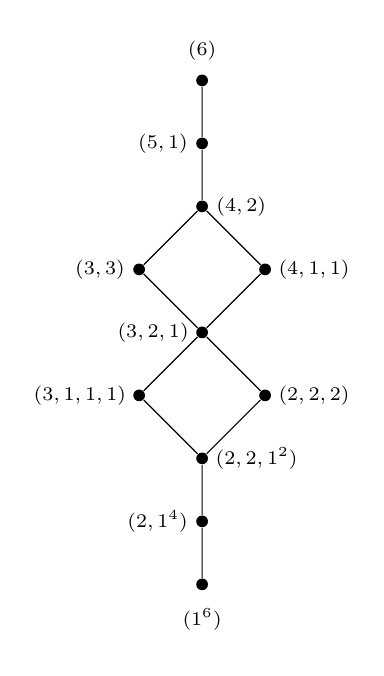
\begin{tikzpicture}[every node/.style={circle, fill, inner sep=1.5pt},scale=0.8]
\node[label=above:{\scriptsize$(6)$}] (6) at (0,8) {};
\node[label=left:{\scriptsize$(5,1)$}] (51) at (0,7) {};
\node[label=right:{\scriptsize$(4,2)$}] (42) at (0,6) {};
\node[label=left:{\scriptsize$(3,3)$}] (33) at (-1,5) {};
\node[label=right:{\scriptsize$(4,1,1)$}] (411) at (1,5) {};
\node[label=left:{\scriptsize$(3,2,1)$}] (321) at (0,4) {};
\node[label=right:{\scriptsize$(2,2,2)$}] (222) at (1,3) {};
\node[label=left:{\scriptsize$(3,1,1,1)$}] (3111) at (-1,3) {};
\node[label=right:{\scriptsize$(2,2,1^2)$}] (2211) at (0,2) {};
\node[label=left:{\scriptsize$(2,1^4)$}] (21111) at (0,1) {};
\node[label=below:{\scriptsize$(1^6)$}] (111111) at (0,0) {};

\draw (111111)--(21111)--(2211)--(222)--(321)--(411)--(42)--(51)--(6);
\draw (2211)--(3111)--(321);
\draw (321)--(33)--(42);
\end{tikzpicture}
\] 

\begin{definition}
    \label{def:lex_order}
    Για δύο (διαφορετικές) διαμερίσεις $\lambda$ και $\mu$ του $n$, γράφουμε $\lambda >_\lex \mu$ και λέμε ότι η $\lambda$ είναι \defn{λεξικογραφικά μεγαλύτερη} της $\mu$ αν για το μικρότερο $i \ge 1$ για το οποίο $\lambda_i \neq \mu_i$ ισχύει ότι $\lambda_i > \mu_i$.
\end{definition}

Το ζεύγος $(\Par(n),<_\lex)$ είναι μια ολική διάταξη η οποία επεκτείνει\footnote{Μια ολική διάταξη η οποία επεκτείνει μια μερική διάταξη ονομάζεται \emph{γραμμική επέκταση} (linear extension).} την διάταξη κυριαρχίας, δηλαδή 
\[
\lambda \triangleright \mu \ \then \ \lambda >_\lex \mu,
\]
για κάθε δύο διαμερίσεις $\lambda, \mu \in \Par(n)$ (γιατί;). Στο παράδειγμα, για $n=6$ έχουμε 
\[
(1^6) <_\lex \cdots <_\lex (2,2,2) <_\lex (3,1^3) <_\lex (3,2,1) <_\lex (3,3) <_\lex (4,1,1) <_\lex \cdots <_\lex (6).
\]

Η Πρόταση~\ref{prop:dominance_lemma} μας πληροφορεί ότι αν $T$ και $Q$ είναι ταμπλώ σχήματος $\lambda$ και $\mu$ τέτοια ώστε $\nabla_T^-[Q] \neq 0$, τότε $\lambda \tge \mu$. Αυτό έχει ως συνέπεια το εξής.

\begin{proposition}
    \label{prop:hom_specht_young}
    Έστω $\lambda, \mu \vdash n$. Αν $\varphi \in \Hom_{\fS_n}(\sS^\lambda,\rmM^\mu)$ είναι μη μηδενική, τότε $\lambda \tge \mu$. Ειδικότερα, αν $\lambda = \mu$, τότε $\varphi = c\,\rmid$, για κάποιο $c \in \CC$.
\end{proposition}

\begin{proof}[Απόδειξη]
    Αν $\varphi \in \Hom_{\fS_n}(\sS^\lambda,\rmM^\mu)$ είναι μη μηδενική, τότε υπάρχει ταμπλώ $T$ σχήματος $\lambda$ τέτοιο ώστε $\varphi(\bfe_T) \neq 0$. Επεκτείνουμε την $\varphi$ σε ολόκληρο το $\rmM^\lambda = \sS^\lambda \oplus (\sS^\lambda)^\perp$, θέτοντας $\varphi((\sS^\lambda)^\perp) = 0$. Έτσι, μπορούμε να γράψουμε 
    \[
    \varphi([T]) = c_1[Q_1] + c_2[Q_2] + \cdots + c_k[Q_k],
    \]
    για κάποια ταμπλοειδή $[Q_i]$ σχήματος $\mu$ και κάποια $c_i \in \CC$. Συνεπώς, 
    \begin{align*}
    \varphi(\bfe_T) 
    &= \varphi(\nabla_T^-[T]) \\
    &= \nabla_T^-\varphi([T]) \\
    &= \nabla_T^-\left(c_1[Q_1] + c_2[Q_2] + \cdots + c_k[Q_k]\right) \\
    &= c_1\nabla_T^-[Q_1] + c_2\nabla_T^-[Q_2] + \cdots + c_k\nabla_T^-[Q_k],
    \end{align*}
    όπου η δεύτερη ισότητα έπεται από το ότι η $\varphi$ είναι $\fS_n$-ομομορφισμός. Επειδή $\varphi(\bfe_T) \neq 0$, υπάρχει κάποιο $1 \le i \le k$, για το οποίο $c_i\nabla_T^-[Q_i] \neq 0$ και κατά συνέπεια $\nabla_T^-[Q_i] \neq 0$. Από την συζήτηση πριν την Πρόταση \ref{prop:hom_specht_young} έπεται ότι $\lambda \tge \mu$.

    Αν $\lambda = \mu$, τότε από το Λήμμα 11.7 (4) έπεται ότι 
    \[
    \varphi(\bfe_T) = c_1\nabla_T^-[Q_1] + c_2\nabla_T^-[Q_2] + \cdots + c_k\nabla_T^-[Q_k] = c\,\bfe_T
    \]
    για κάποιο $c \in \CC$. Το ζητούμενο έπεται από την κυκλικότητα του $\sS^\lambda$.
\end{proof}

\begin{theorem}
    \label{thm:specht_irreducible_complete_set}
    Το 
    $
    \{\sS^\lambda : \lambda \vdash n\}
    $
    αποτελεί ένα σύνολο αν δύο μη ισόμορφων ανάγωγων $\fS_n$-προτύπων.
\end{theorem}

\begin{proof}[Απόδειξη]
    Από το Πόρισμα 11.6 γνωρίζουμε ότι κάθε πρότυπο Specht είναι ανάγωγο. Επίσης, αν $\lambda \neq \mu$, τότε προφανώς $\sS^\lambda \ncong_{\fS_n} \sS^\mu$. Συνεπώς, αρκεί να αποδείξουμε ότι αν $\sS^\lambda \cong_{\fS_n} \sS^\mu$, τότε $\lambda = \mu$. Αυτό είναι άμεση συνέπεια της Πρότασης \ref{prop:hom_specht_young}.

    Πράγματι, αν $\sS^\lambda \cong_{\fS_n} \sS^\mu$, τότε $\Hom_{\fS_n}(\sS^\lambda,\sS^\mu) \neq \{0\}$ και γι αυτό $\lambda \tge \mu$. Επίσης, $\Hom_{\fS_n}(\sS^\mu, \sS^\lambda) \neq \{0\}$ και γι αυτό $\mu \tge \lambda$. Άρα, $\lambda = \mu$.
\end{proof}

Το Θεώρημα \ref{thm:specht_irreducible_complete_set} μας πληροφορεί ότι η ολική διάταξη του $\Par(n)$ που ψάχναμε είναι η λεξικογραφική διάταξη (ή, πιο σωστά, η \textquote{ανάποδή} της). Έτσι ολοκληρώνεται το πρόγραμμα που ξεκινήσαμε στην αρχή της παραγράφου.
\begin{corollary}
    \label{cor:young_rule_repTheoretic}
    Για $\mu \vdash n$, η ισοτυπική διάσπαση του προτύπου Young δίνεται από 
    \begin{equation}
        \label{eq:young_rule}
        \rmM^\mu \cong_{\fS_n} \bigoplus_{\lambda \ge_{\lex} \mu} \left(\sS^\lambda\right)^{m_{\lambda\mu}},
    \end{equation}
    όπου $m_{\lambda\mu} \in \NN$ με $m_{\lambda\lambda} = 1$.
\end{corollary}

\begin{proof}[Απόδειξη]
    Από το Θεώρημα~\ref{thm:specht_irreducible_complete_set} έπεται ότι 
    \[
    \rmM^\mu \cong_{\fS_n} \bigoplus_{\lambda \vdash n} \left(\sS^\lambda\right)^{m_{\lambda\mu}},
    \]
    όπου 
    \[
    m_{\lambda\mu} = \dim\left(\Hom_{\fS_n}(\sS^\lambda,\rmM^\mu)\right),
    \]
    από το Λήμμα \ref{lem:Schur_uniqueness_of_isotypic_decomposition}. Το ζητούμενο έπεται από την Πρόταση \ref{prop:hom_specht_young}.
\end{proof}

Οι αριθμοί $m_{\lambda\mu}$ που εμφανίζονται στην Ταυτότητα \eqref{eq:young_rule} ονομάζονται \defn{αριθμοί Kostka}. Είναι φυσικό να αναρωτηθεί κανείς τι απαριθμούν. Αργότερα, θα δούμε μια συνδυαστική τους ερμηνεία. Για την ώρα, χρησιμοποιώντας κανείς τον πίνακα χαρακτήρων της $\fS_4$ μπορεί να υπολογίσει τον πίνακα $(m_{\lambda\mu})_{\lambda,\mu \, \vdash 4}$, ο οποίος είναι 
\[
\renewcommand{\arraystretch}{1.2}
\begin{array}{c|ccccc}
              & (4) & (3,1) & (2,2) & (2,1,1) & (1,1,1,1) \\\hline
    (4)       & 1   & 0     & 0     & 0       & 0 \\
    (3,1)     & 1   & 1     & 0     & 0       & 0 \\
    (2,2)     & 1   & 2     & 1     & 0       & 0 \\
    (2,1,1)   & 1   & 2     & 1     & 1       & 0 \\
    (1,1,1,1) & 1   & 3     & 2     & 3       & 1 \\
\end{array}.
\]
Ποιός είναι ο αντίστοιχος πίνακας για $n=5$;

\section{Συνήθη Young ταμπλώ και το θεώρημα βάσης}
\label{sec:SYT}

Από τον Ορισμό \ref{def:polytabloid} δεν μπορούμε να αποφανθούμε ποιά είναι η διάσταση ενός προτύπου Specht, καθώς εν γένει υπάρχουν γραμμικές σχέσεις που ικανοποιούνται από πολυταμπλοειδή ίδιου σχήματος. Συνεπώς, είναι φυσικό να αναρωτηθεί κανείς το εξής.
\begin{que}
    Ποιά πολυταμπλοειδή αποτελούν βάση ενός προτύπου Specht και πόσα είναι αυτά;
\end{que}

Για $\lambda = (2,1) \vdash 3$, στο Παράδειγμα \ref{ex:specht_modules} (1), είδαμε ότι το 
\[
\ytableausetup{smalltableaux,notabloids}
\sS^{(2,1)} = \CC[\bfe_{\ytableaushort{12, 3}}\, , \bfe_{\ytableaushort{13, 2}} \,]
\]
είναι ισόμορφο με την συνήθη αναπαράσταση της $\fS_3$ και γι αυτό $\dim(\sS^{(2,1)}) = 2$. Οι γραμμικές σχέσεις που ικανοποιούν τα υπόλοιπα τέσσερα πολυταμπλοειδή είναι 
\begin{align*}
    \bfe_{\ytableaushort{21, 3}} \ 
    &= \ \bfe_{\ytableaushort{12, 3}} - \bfe_{\ytableaushort{13, 2}} \\
    \bfe_{\ytableaushort{31, 2}} \ 
    &= \ \bfe_{\ytableaushort{13, 2}} - \bfe_{\ytableaushort{12, 3}} \\ 
    \bfe_{\ytableaushort{23, 1}} \
    &= \ - \bfe_{\ytableaushort{13, 2}} \\ 
    \bfe_{\ytableaushort{32, 1}} \
    &= \ - \bfe_{\ytableaushort{12, 3}} \\ 
\end{align*}
(γιατί;). 

\begin{definition}
    \label{def:SYT}
    Έστω $\lambda \vdash n.$ Ένα Young ταμπλώ σχήματος $\lambda$ ονομάζεται \defn{σύνηθες} (standard) αν 
    \begin{itemize}
        \item τα στοιχεία της κάθε γραμμής του αυξάνουν από αριστερά προς τα δεξιά\footnote{Στην περίπτωση αυτή λέμε ότι το ταμπλώ είναι \emph{row-standard}.}, και
        \item τα στοιχεία της κάθε στήλης του αυξάνουν από πάνω προς τα κάτω\footnote{Στην περίπτωση αυτή λέμε ότι το ταμπλώ είναι \emph{column-standard}.}.
    \end{itemize}
    Έστω $\SYT(\lambda)$ το σύνολο των συνήθων Young ταμπλώ σχήματος $\lambda$.
\end{definition}

Ένα παράδειγμα συνήθους ταμπλώ σχήματος $(4,2,2,1)$ είναι 
\[
\ytableausetup{nosmalltableaux,centertableaux}
\begin{ytableau}
1 & 3 & 7 & 8 \\
2 & 5 \\
4 & 9 \\
6 \\
\end{ytableau}.
\]

\begin{example}
Έστω $f^\lambda \coloneqq \abs{\SYT(\lambda)}$.
\begin{itemize}
    \item[(1)] Προφανώς, $f^{(n)} = f^{(1^n)} = 1$.
    \item[(2)] Έχουμε $f^{(n-1,1)} = n-1$, διότι από την πρώτη συνθήκη του Ορισμού \ref{def:SYT}, η επιλογή του στοιχείου της δεύτερης γραμμής καθορίζει ένα σύνηθες ταμπλώ σχήματος $(n-1,1)$ (γιατί;). Γενικότερα\footnote{Με $\binom{n}{k}$ συμβολίζουμε το πλήθος των υποσυνόλων του $[n]$ με $k$ στοιχεία. Οι ακέραιοι $\binom{n}{k}$ ονομάζονται \defn{διωνυμικοί συντελεστές}.}, 
    \[
    f^{(n-k,1^k)} = \binom{n-1}{k}.
    \] 
    \item[(3)] Τα συνήθη ταμπλώ σχήματος $(3,3)$ είναι  
    \[
    \ytableaushort{123,456} \, , \quad
    \ytableaushort{124,356} \, , \quad 
    \ytableaushort{125,346} \, , \quad 
    \ytableaushort{134,256} \, , \quad 
    \ytableaushort{135,246} \, 
    \]
    και γι αυτό $f^{(3,3)} = 5$. Γενικότερα\footnote{Ο αριθμός $\frac{1}{n+1}\binom{2n}{n}$ ονομάζεται $n$-οστός \defn{αριθμός Catalan}.},
    \[
    f^{(n,n)} = \frac{1}{n+1}\binom{2n}{n}.
    \]
\end{itemize}
\end{example}

\begin{theorem}{\rm(Θεώρημα βάσης)}
    \label{thm:basis_thm}
    Έστω $\lambda \vdash n$. Το σύνολο 
    \[
    \{\bfe_T : T \in \SYT(\lambda)\}
    \]
    αποτελεί βάση του προτύπου Specht $\sS^\lambda$. Ειδικότερα,
    \[
    \dim(\sS^\lambda) = f^\lambda.
    \]
\end{theorem}

Για να προετοιμαστούμε για την απόδειξη του Θεωρήματος \ref{thm:basis_thm}, εισάγουμε μια διάταξη στο σύνολο των ταμπλειδών ίδιου σχήματος.

\begin{definition}
    \label{def:young_last_letter_order}
    Έστω $T$ και $Q$ δύο ταμπλώ ίδιου σχήματος. Γράφουμε $[T] < [Q]$ αν 
    \begin{itemize}
        \item υπάρχει $i \in [n]$, τέτοιο ώστε $r_T(i) \neq r_Q(i)$
        \item για το μεγαλύτερο τέτοιο $i$ ισχύει ότι $r_T(i) < r_Q(i)$.
    \end{itemize}
\end{definition}

Με άλλα λόγια, $[T] < [Q]$ αν και μόνο αν το μεγαλύτερο στοιχέιο που εμφανίζεται σε διαφορετικές γραμμές των $T$ και $Q$ βρίσκεται βορειότερα στο $[T]$ από ότι στο $[Q]$. Για παράδειγμα, 
\[
\ytableausetup{tabloids}
\begin{ytableau}
2 & 3 & 7 \\
4 & *(burntorange)6 \\
1 & 5 
\end{ytableau} 
\ < \ 
\ytableausetup{tabloids}
\begin{ytableau}
3 & 5 & 7 \\
1 & 4 \\
2 & *(burntorange)6 
\end{ytableau} \ .
\]
Η σχέση $<$ αποτελεί ολική διάταξη στο σύνολο των ταμπλειδών ίδιου σχήματος. Το ταμπλοειδές που βρίσκεται  χαμηλότερα σε αυτή τη διάταξη, έχει τα μεγαλύτερα στοιχεία του συγκεντρωμένα σε υψηλότερες γραμμές. Για παράδειγμα, για $\lambda = (2,2)$ έχουμε 
\[
\ytableausetup{nosmalltableaux}
\ytableaushort{34,12} \ < \
\ytableaushort{24,13} \ < \
\ytableaushort{14,23} \ < \
\ytableaushort{23,14} \ < \
\ytableaushort{13,24} \ < \
\ytableaushort{12,34} \ .
\]

\begin{lemma}
    \label{lem:basis_thm}
    Αν $T$ είναι ταμπλώ σχήματος  $\lambda \vdash n$, τέτοιο ώστε τα στοιχεία της κάθε στήλης του $T$ να αυξάνουν από πάνω προς τα κάτω, τότε
    \begin{itemize}
        \item[(1)] υπάρχει μια μετάθεση $\pi \in \rmC(T)$ με $\pi \neq \epsilon$ για την οποία $[\pi{T}] < [T]$, και
        \item[(2)] $\bfe_T = [T] +  \left(\text{γραμμικός συνδυασμός ταμπλοειδών $[Q]$ σχήματος $\lambda$ με $[Q] < [T]$}\right)$. 
    \end{itemize}
\end{lemma}

\begin{proof}[Απόδειξη]
    Το (2) έπεται άμεσα από το (1), διότι 
    \begin{align*}
        \bfe_T 
        = \nabla_T^-[T] 
        = \sum_{\pi \in \rmC(T)} \sign(\pi) [\pi{T}] 
        = [T] + \sum_{\substack{\pi \in \rmC(T) \\ \pi \neq \epsilon}} \sign(\pi) \underbrace{[\pi{T}]}_{< \ [T]}.
    \end{align*}

    Για το (1), έστω $\pi \in \rmC(T)$ με $\pi \neq \epsilon$. Θεωρούμε τον μεγαλύτερο ακέραιο $k \in [n]$ τέτοιο ώστε $\pi(k) \neq k$. Κάθε στοιχείο νότια του $k$ στο $T$ μένει σταθερό στο $\pi{T}$ και το $k$ μετατίθεται βορειότερα (γιατί;). Άρα, $[\pi{T}] < [T]$. 
    
    Για παράδειγμα, αν
    \[
    \ytableausetup{notabloids}
    T = \
    \begin{ytableau}
        1 & 3 & 5 & 4 \\
        2 & *(burntorange)6 & 7 \\
        9 & *(iceberg)8 
    \end{ytableau} 
    \quad 
    \text{και}
    \quad
    \pi = \cycle{3,6}
    \]
    με $k=6$, τότε
    \[
    \pi{T} = \
    \begin{ytableau}
        1 & *(burntorange)6 & 5 & 4 \\
        2 & 3 & 7 \\
        9 & *(iceberg)8 
    \end{ytableau}
    \]
    και γι αυτό 
    \[
    \ytableausetup{tabloids}
    [\pi{T}] = \ 
    \begin{ytableau}
        1 & *(burntorange)6 & 5 & 4 \\
        2 & 3 & 7 \\
        9 & 8 
    \end{ytableau}
    \ < \ 
    \begin{ytableau}
        1 & 3 & 5 & 4 \\
        2 & *(burntorange)6 & 7 \\
        9 & 8 
    \end{ytableau} 
    \ = [T].
    \]
\end{proof}

θα χρησιμοποιήσουμε το Λήμμα \ref{lem:basis_thm} για να αποδείξουμε το θεώρημα βάσης.

\begin{proof}[Απόδειξη του Θεωρήματος~\ref{thm:basis_thm}]
    Θα δείξουμε ότι το σύνολο $\{\bfe_T : T \in \SYT(\lambda)\}$ είναι γραμμικώς ανεξάρτητο υποσύνολο του $\rmM^\lambda$. Για τον σκοπό αυτό, υποθέτουμε ότι 
    \[
    c_{T_1} \bfe_{T_1} + c_{T_2} \bfe_{T_2} + \cdots + c_{T_k} \bfe_{T_k} = 0 \quad \text{στο $\rmM^\lambda$},
    \]
    για κάποια $c_{T_1}, c_{T_2}, \dots, c_{T_k} \neq 0$ και $T_1, T_2, \dots, T_k \in \SYT(\lambda)$. Έστω $T_{\max}$ το σύνηθες ταμπλώ εκ των $T_1, T_2, \dots, T_k$ του οποίου το αντίστοιχο ταμπλειδές είναι το μεγαλύτερο ως προς τη διάταξη του Ορισμού \ref{def:young_last_letter_order}. 
    \begin{claim}
        Για κάθε $1 \le i \le k$, αν 
        \[
        \bfe_{T_i} = \sum_{[Q]} a_{[Q]}^i [Q],
        \]
        όπου στο άθροισμα το $[Q]$ διατρέχει όλα τα ταμπλοειδή σχήματος $\lambda$, για $a_{[Q]}^i \in \CC$, τότε 
        \[
        a_{[T_{\max}]}^i = 
        \begin{cases}
            1, &\ \text{αν $T_i = T_{\max}$} \\
            0, &\ \text{διαφορετικά} \\
        \end{cases}. 
        \]
    \end{claim}
    O ισχυρισμός έπεται άμεσα από το Λήμμα \ref{lem:basis_thm}. Πράγματι, το (2) του λήμματος μας πληροφορεί ότι 
    \[
    \bfe_{T_i} = 
    [T_i] + \ \left(\text{γραμμικός συνδυασμός ταμπλοειδών $[Q]$ σχήματος $\lambda$ με $[Q] < [T_i]$}\right)
    \]
    Συνεπώς, το $[T_{\max}]$ θα εμφανιστεί στο ανάπτυγμα κάποιου $\bfe_{T_i}$ μόνο αν $T_i = T_{\max}$ και σε αυτή την περίπτωση με συντελεστή 1 (γιατί;).

    Από τον ισχυρισμό, ο συντελεστής του $[T_{\max}]$ στο ανάπτυγμα του 
    \[
    c_{T_1} \bfe_{T_1} + c_{T_2} \bfe_{T_2} + \cdots + c_{T_k} \bfe_{T_k} \ \in \ \rmM^\lambda
    \]
    στην βάση των ταμπλοδειδών σχήματος $\lambda$ ισούται με 
    \[
    \sum_{i=1}^k c_{T_i}a_{[T_{\max}]}^i = c_{T_{\max}} \neq 0.
    \]
    Αυτό όμως είναι αδύνατο, διότι 
    \[
    c_{T_1} \bfe_{T_1} + c_{T_2} \bfe_{T_2} + \cdots + c_{T_k} \bfe_{T_k} = 0.
    \]

    Για να ολοκληρωθεί η απόδειξη, μένει να δείξουμε ότι το σύνολο $\{\bfe_T : T \in \SYT(\lambda)\}$ παράγει το $\sS^\lambda$. Από την Ταυτότητα \eqref{eq:dimension_formula}, έπεται ότι
    \[
    n! = \sum_{\lambda \vdash n} \dim(\sS^\lambda)^2 \ge \sum_{\lambda \vdash n} (f^\lambda)^2,
    \]
    όπου η τελευταία ανισότητα έπεται από την γραμμική ανεξαρτησία του $\{\bfe_T : T \in \SYT(\lambda)\}$. Το ζητούμενο, δηλαδή ότι $\dim(\sS^\lambda) = f^\lambda$, έπεται από το Θεώρημα \ref{thm:RS_correspondence}\footnote{Για μια κατασκευαστική απόδειξη, θα έπρεπε να ξεκινήσουμε με ένα πολυταμπλοειδές $\bfe_T$ για κάποιο ταμπλώ $T$ και να δείξουμε ότι μπορεί να γραφεί ως γραμμικός συνδυασμός πολυταμπλοειδών $\bfe_Q$ για συνήθη ταμπλώ $Q$. Μια τέτοια απόδειξη δόθηκε από τον Garnir το 1950, επινοώντας έναν αλγόριθμο για να το κάνει αυτό, ο οποίος σήμερα ονομάζεται \emph{straightening algorithm} (βλ. \cite[Ενότητα~2.6]{Sag01}).}.
\end{proof}

Θα περιγράψουμε τώρα, μια αντιστοιχία από το σύνολο των μεταθέσεων της $\fS_n$ στο σύνολο όλων των ζευγών συνήθων ταμπλώ ίδιου σχήματος και περιεχομένου $[n]$. Αυτή βασίζεται στον λεγόμενο \emph{αλγόριθμο εισαγωγής γραμμών} (row insertion algorithm). 

Έστω $T$ ταμπλώ και έστω $x$ θετικός ακέραιος ο οποίος δεν είναι στοιχείο του $T$. Έστω $T \leftarrow x$ το ταμπλώ που ορίζεται ως εξής: 
\begin{itemize}
    \item Αν το $x$ είναι μεγαλύτερο από όλα τα στοιχεία της πρώτης γραμμής, τότε το $T \leftarrow x$ είναι το ταμπλώ που προκύπτει προσθέτοντας ένα τετράγωνο στο τέλος της πρώτης γραμμής του $T$ με το $x$ στο εσωτερικό του. 
    \item Διαφορετικά, έστω $y$ το μικρότερο στοιχείο της πρώτης γραμμής του $T$ για το οποίο $y > x$. Αντικαθιστούμε το $y$ με το $x$ και επαναλαμβάνουμε τη διαδικασία για το $y$ και τη δεύτερη γραμμή. Το $T \leftarrow x$ είναι το ταμπλώ που προκύτπει στο τέλος αυτής της διαδικασίας.
\end{itemize}

Για παράδειγμα, για
\[
\ytableausetup{notabloids,centertableaux}
Τ \ = \ 
\begin{ytableau}
1 & 3 & 8 \\
5 & 9 \\ 
6 \\
7
\end{ytableau}
\quad \text{και} \quad 
x = 4,
\]
ο αλγόριθμος εισαγωγής του $x$ στις γραμμές του $T$ έχει τα εξής βήματα:
\begin{itemize}
    \item Βρίσκουμε το μικρότερο στοιχείο της πρώτης γραμμής το οποίο είναι μεγαλύτερο από το 4
    \[
    \begin{ytableau}
    1 & 3 & *(burntorange) 8 \\
    5 & 9 \\ 
    6 \\
    7
    \end{ytableau}
    \]
    και το αντικαθιστούμε με το 4 
    \[
    \begin{ytableau}
    1 & 3 & 4 \\
    5 & 9 \\ 
    6 \\
    7
    \end{ytableau} \ .
    \]

    \item Βρίσκουμε το μικρότερο στοιχείο της δεύτερης γραμμής το οποίο είναι μεγαλύτερο από το 8
    \[
    \begin{ytableau}
    1 & 3 & 4 \\
    5 & *(burntorange) 9 \\ 
    6 \\
    7
    \end{ytableau}
    \]
    και το αντικαθιστούμε με το 8 
    \[
    \begin{ytableau}
    1 & 3 & 4 \\
    5 & 8 \\ 
    6 \\
    7
    \end{ytableau} \ .
    \]

    \item Το 9 είναι μεγαλύτερο από όλα τα στοιχεία της τρίτης γραμμής και γι αυτό 
    \[
    T \leftarrow x \ = \
    \begin{ytableau}
    1 & 3 & 4 \\
    5 & 8 \\ 
    6 & 9 \\
    7
    \end{ytableau} \ .
    \]
\end{itemize}

Για $\pi = \pi_1\pi_2\cdots\pi_n \in \fS_n$, έστω 
\[
\rmP(\pi) \coloneqq 
\left(
    \left( \cdots
        \left(
            \emptyset \leftarrow \pi_1
        \right) \leftarrow \pi_2
    \right) \leftarrow \cdots 
\right) \leftarrow \pi_n.
\]
Το $\rmP(\pi)$ είναι ένα σύνηθες ταμπλώ περιεχομένου $[n]$, το οποίο ονομάζεται \defn{ταμπλώ εισαγωγής} (insertion tableau) της $\pi$. Έστω, επίσης, $\rmQ(\pi)$ το σύνηθες ταμπλώ περιεχομένου $[n]$ στο οποίο, για κάθε $i \in [n]$, το στοιχείο $i$ καταλαμβάνει τη θέση στην οποία τερματίζεται η εισαγωγή του $\pi_i$ στο ταμπλώ 
\[
\left(
    \left( \cdots
        \left(
            \emptyset \leftarrow \pi_1
        \right) \leftarrow \pi_2
    \right) \leftarrow \cdots 
\right) \leftarrow \pi_{i-1}. 
\]
Το $\rmQ(\pi)$ είναι ένα σύνηθες ταμπλώ περιεχομένου $[n]$ ίδιου σχήματος με το $\rmP(\pi)$, το οποίο ονομάζεται \defn{ταμπλώ καταγραφής} (recording tableau) της $\pi$.

Για παράδειγμα, για $\pi = 765193842 \in \fS_9$, έχουμε τα ακόλουθα βήματα κατασκευής των ταμπλώ εισαγωγής και καταγραφής:
\[
\renewcommand{\arraystretch}{2}
\begin{array}{ccccc}
\left( \
    \ytableaushort{7} \, ,\, \ytableaushort{1} \
\right)
& \rightsquigarrow &
\left( \
    \ytableaushort{6,7} \, ,\, \ytableaushort{1,2} \
\right)
& \rightsquigarrow &
\left( \
    \ytableaushort{5,6,7} \, ,\, \ytableaushort{1,2,3} \
\right) \\[25pt] 
\left( \
    \ytableaushort{1,5,6,7} \, ,\, \ytableaushort{1,2,3,4} \
\right)
& \rightsquigarrow &
\left( \
    \ytableaushort{19,5,6,7} \, ,\, \ytableaushort{15,2,3,4} \
\right)
& \rightsquigarrow &
\left( \
    \ytableaushort{13,59,6,7} \, ,\, \ytableaushort{15,26,3,4} \
\right) \\[35pt]
\left( \
    \ytableaushort{138,59,6,7} \, ,\, \ytableaushort{157,26,3,4} \
\right) 
& \rightsquigarrow &
\left( \
    \ytableaushort{134,58,69,7} \, ,\, \ytableaushort{157,26,38,4} \
\right) \, .
\end{array}
\]

\begin{theorem}{\rm(Robinson 1936, Schensted 1961)}
    \label{thm:RS_correspondence}
    Η απεικόνιση $\pi \mapsto \left(\rmP(\pi), \rmQ(\pi)\right)$ είναι αμφιμονοσήμαντη. Ειδικότερα,
    \[
    n! = \sum_{\lambda \vdash n} (f^\lambda)^2.
    \]
\end{theorem}

Η απεικόνιση αυτή ονομάζεται \emph{αντιστοιχία Robinson--Schensted}. Όπως είδαμε, το Θεώρημα \ref{thm:basis_thm} μπορεί να αποδειχθεί χωρίς την χρήση του Θεωρήματος $\ref{thm:RS_correspondence}$. Έχοντας αυτό κατά νου, η αντιστοιχία Robinson--Schensted δίνει μια συνδυαστική απόδειξη του τύπου διάστασης για την συμμετρική ομάδα. Για μία απόδειξη του Θεωρήματος \ref{thm:RS_correspondence} παραπέμπουμε στο \cite[Θεώρημα 3.1.1]{Sag01}.

Ολοκληρώνουμε την παρούσα παράγραφο, παρουσιάζοντας έναν τύπο για την διάσταση του προτύπου Specht.
\begin{definition}
    \label{def:hook_length}
    Έστω $\lambda \vdash n$. Για ένα τετράγωνο $x$ του $\rmY_\lambda$, το οποίο συμβολικά γράφουμε $x \in \rmY_\lambda$, το σύνολο $\rmH(x)$ των τετραγώνων που βρίσκονται ασθενώς ανατολικά ή ασθενώς νότια του $x$ στο $\rmY_\lambda$ ονομάζεται \defn{γάντζος} (hook) του $x$. Θέτουμε $\rmh(x) \coloneqq \abs{\rmH(x)}$. 
\end{definition}

Για παράδειγμα, για $\lambda = (4,2,2,1)$ ο γάντζος του τετραγώνου $x$  
\[
\ytableausetup{notabloids}
\rmY_{(4,2,2,1)} = 
\begin{ytableau}
    {} & x & {} & {} \\
    {} & {} \\
    {} & {} \\
    {}
\end{ytableau}
\]
που βρίσκεται στη θέση (1,2) είναι 
\[
\ydiagram{4,2,2,1}
*[*(burntorange)]{1+1,1+1,1+1}
*[*(burntorange)]{2+2}
\]
και γι αυτό $\rmh(x) = 5$.

Το επόμενο αποτέλεσμα, γνωστό ως \emph{hook length formula}, δίνει έναν αναπάντεχα απλό\footnote{Δεν υπάρχει κανένας προφανής λόγος που να εξηγεί το ότι ο αριθμός στο δεξί μέλος της Ταυτότητας \eqref{eq:hook_length_formula} είναι ακέραιος.} τύπο για το πλήθος των συνήθων ταμπλώ δοσμένου σχήματος, και κατ' επέκταση τη διάσταση του προτύπου Specht. 
\begin{theorem}{\rm(Frame--Robinson--Thrall 1954)}
    \label{thm:hook_length_formula}
    Για $\lambda \vdash n$, 
    \begin{equation} 
        \label{eq:hook_length_formula}
        f^\lambda = 
        \frac{n!}{\prod_{x \in \rmY_\lambda} \rmh(x)}.
    \end{equation}
\end{theorem}

Το Θεώρημα \ref{thm:hook_length_formula} έχει μια πληθώρα διαφορετικών αποδείξεων. Για μερικές από αυτές παραπέμπουμε στο \cite[Ενότητες 14.5.1 και 14.6]{AR15}.

Για παράδειγμα, ας υπολογίσουμε το πλήθος των συνήθων ταμπλώ σχήματος $\lambda = (4,2,$ $2,1)$, χρησιμοποιώντας την Ταυτότητα \eqref{eq:hook_length_formula}. Για να το κάνουμε αυτό, γεμίζουμε τα τετράγωνα του διαγράμματος Young της $\lambda$ με τα μήκη κάθε γάντζου του αντίστοιχου τετραγώνου ως εξής 
\[
\begin{ytableau}
    7 & 5 & 2 & 1 \\
    4 & 2 \\
    3 & 1 \\
    1
\end{ytableau} \, .
\]
Τότε, η Ταυτότητα~\eqref{eq:hook_length_formula} μας πληροφορεί ότι 
\[
f^{(4,2,2,1)} = \frac{9!}{1^3\cdot2^3\cdot3\cdot4\cdot5\cdot7} = 108.
\]

\section{Κανόνες διακλάδωσης}
\label{sec:branching_rules}

Στο Παράδειγμα \ref{ex:induction_of_trivial_defining}, είδαμε ότι 
\[
\rmM^{(n-1)}\uparrow_{\fS_{n-1}}^{\fS_n} \cong_{\fS_n} V^\triv\uparrow_{\fS_{n-1}}^{\fS_n} \cong_{\fS_n} V^\rmdef \cong_{\fS_n} V^\triv \oplus V^\std \cong_{\fS_n} \sS^{(n)} \oplus \sS^{(n-1,1)},
\]
όπου o τελευταίος ισομορφισμός έπεται από το Παράδειγμα \ref{ex:specht_modules} (1).  Παρατηρούμε λοιπόν ότι η ισοτυπική διάσπαση της επαγωγής του προτύπου Specht που αντιστοιχεί στην διαμέριση $(n-1)$ στην $\fS_n$ προκύπτει \textquote{επεκτείνοντας} την $(n-1)$ σε διαμέριση του $n$ με όλους τους πιθανούς τρόπους. Συνεπώς, είναι φυσικό να αναρωτηθεί κανείς το εξής.
\begin{que}
    Για $\lambda \vdash n$, υπάρχει κάποιος απλός, κατά προτίμηση συνδυαστικός, κανόνας για να υπολογίσουμε τις ισοτυπικές διασπάσεις της επαγωγής και του περιορισμού του $\sS^\lambda$ στην $\fS_{n+1}$ και $\fS_{n-1}$, αντίστοιχα;
\end{que}

Για ακόμα μια φορά, η απάντηση είναι αναπάντεχα απλή. Διαισθητικά, η επαγωγή και ο περιορισμός ενός προτύπου Specht αντιστοιχούν σε προσθαφαίρεση τετραγώνων στο διάγραμμα Young της αντίστοιχης διαμέρισης.
\begin{definition}
    \label{def:inne_outer_corner}
    Για $\lambda \vdash n$, έστω $\pP^-(\lambda)$ (αντ. $\pP^+(\lambda)$) το σύνολο των διαμερίσεων του $n-1$ (αντ. $n+1$) των οποίων το διάγραμμα Young προκύπτει από το $\rmY_\lambda$ αφαιρώντας (αντ. προσθέτοντας) ακριβώς ένα τετράγωνο, το οποίο ονομάζεται \defn{εσωτερική} (αντ. \defn{εξωτερική}) \defn{γωνία} της $\lambda$.
\end{definition}

Για παράδειγμα, οι εσωτερικές και εξωτερικές γωνίες της διαμέρισης $(4,2,2,1)$ είναι
\[
\ytableausetup{centertableaux}
\ydiagram{3,2,1}
*[*(burntorange)]{3+1}
*[*(burntorange)]{3+0,2+0,1+1}
*[*(burntorange)]{3+0,2+0,1+0,1}
\quad \text{και} \quad 
\ydiagram{4,2,2,1}
*[*(iceberg)]{4+1}
*[*(iceberg)]{4+0,2+1}
*[*(iceberg)]{4+0,2+0,2+0,1+1}
*[*(iceberg)]{4+0,2+0,2+0,1+0,1}
\]
αντίστοιχα, και γι αυτό 
\begin{align*}
    \pP^-(4,2,2,1) &= \{(3,2,2,1), (4,2,1,1), (4,2,2)\} \ \subseteq \Par(8) \\
    \pP^+(4,2,2,1) &= \{(5,2,2,1), (4,3,2,1), (4,2,2,2), (4,2,2,1,1)\} \ \subseteq \Par(10). \\
\end{align*}

\begin{proposition}
    \label{prop:branching_rule}
    Για κάθε $\lambda \vdash n$, 
    \begin{equation}
        \label{eq:branching_rule_help}
        f^\lambda = \sum_{\mu \in \pP^-(\lambda)} f^\mu.
    \end{equation}
\end{proposition}
\begin{proof}[Απόδειξη]
    Παρατηρούμε ότι σε κάθε σύνηθες ταμπλώ περιεχομένου $[n]$, το στοιχείο $n$ καταλαμβάνει μια εσωτερική γωνία του $\lambda$ (γιατί;). Για παράδειγμα, για $\lambda = (4,2,2,1) \vdash 9 = n$, έχουμε τις εξής επιλογής
    \[
    \begin{ytableau}
    \ast & \ast & \ast & 9 \\
    \ast & \ast  \\
    \ast & \ast  \\
    \ast
    \end{ytableau} 
    \quad \text{ή} \quad 
    \begin{ytableau}
    \ast & \ast & \ast & \ast \\
    \ast & \ast  \\
    \ast & 9  \\
    \ast
    \end{ytableau} 
    \quad \text{ή} \quad 
    \begin{ytableau}
    \ast & \ast & \ast & \ast \\
    \ast & \ast  \\
    \ast & \ast  \\
    9
    \end{ytableau} \, .
    \]
    Αν $r_1, r_2, \dots, r_k$ είναι οι πιθανές εσωτερικές γωνίες της $\lambda$, με τις αντίστοιχες διαμερίσεις του $\pP^-(\lambda)$ να είναι $\mu^1, \mu^2, \dots, \mu^k$, τότε αφαιρώντας κάθε εσωτερική γωνία που κατέχει το στοιχείο $n$ και απαριθμώντας τα συνήθη ταμπλώ περιεχομένου $[n-1]$ που προκύπτουν έπεται ότι 
    \[
    f^\lambda = f^{\mu^1} + f^{\mu^2} + \cdots + f^{\mu^k}
    \]
    το οποίο είναι το ζητούμενο. Στο παράδειγμα, 
    \[
    f^{(4,2,2,1)} = f^{(3,2,2,1)} + f^{(4,2,1,1)} + f^{(4,2,2)}.
    \]
\end{proof}

\begin{theorem}{\rm(Κανόνες διακλάδωσης)}
    \label{thm:branching_rules}
    Για κάθε $\lambda \vdash n$, 
    \begin{align}
        \label{eq:branching_restriction}
        \sS^\lambda\!\downarrow_{\fS_{n-1}}^{\fS_n} 
        &\cong_{\fS_{n-1}} \bigoplus_{\mu \in \pP^-(\lambda)} \sS^\mu \\
        \label{eq:branching_induction}
        \sS^\lambda\!\uparrow_{\fS_n}^{\fS_{n+1}} 
        &\cong_{\fS_{n+1}} \bigoplus_{\mu \in \pP^+(\lambda)} \sS^\mu. 
    \end{align}
\end{theorem}

Για την διαμέριση του τρέχοντος παραδείγματος, οι κανόνες διακλάδωσης μας πληροφορούν ότι 
\begin{align*}
    \sS^{(4,2,2,1)}\!\downarrow_{\fS_8}^{\fS_9} 
    &\cong_{\fS_8} \sS^{(3,2,2,1)} \oplus \sS^{(4,2,1,1)} \oplus \sS^{(4,2,2)}\\
    \sS^{(4,2,2,1)}\!\uparrow_{\fS_9}^{\fS_{10}}  
    &\cong_{\fS_{10}} \sS^{(5,2,2,1)} \oplus \sS^{(4,3,2,1)} \oplus \sS^{(4,2,2,2)} \oplus \sS^{(4,2,2,1,1)}.
\end{align*}
Η απόδειξη που θα δούμε έχει το πλεονέκτημα ότι είναι ανεξάρτητη από το σώμα πάνω από το οποίο δουλεύουμε.
\begin{proof}[Απόδειξη του Θεωρήματος~\ref{thm:branching_rules} \rm(Peel 1975)]    
    Αρχικά, συνδυάζοντας τα Θεωρήματα \ref{thm:orthogonality_rels_I} και \ref{thm:frobenius_reciprocity_law}, αρκεί να αποδείξουμε την μία από τις δύο ταυτότητες. Πράγματι, ας υποθέσουμε ότι ισχύει η Ταυτότητα~\eqref{eq:branching_restriction}. Αν $\chi^\lambda$ είναι ο χαρακτήρας του $\sS^\lambda$, τότε για κάθε $\nu \vdash n+1$
    \begin{align*}
        \left(\chi^\lambda\!\uparrow_{\fS_n}^{\fS_{n+1}}, \chi^\nu\right)_{\fS_{n+1}} 
        &= \left(\chi^\lambda, \chi^\nu\!\downarrow_{\fS_n}^{\fS_{n+1}}\right)_{\fS_n} \\
        &= \left(\chi^\lambda, \sum_{\mu \in \pP^-(\nu)} \chi^\mu\right)_{\fS_n} \\
        &= 
        \begin{cases}
            1, &\ \text{αν $\lambda \in \pP^-(\nu)$} \\
            0, &\ \text{διαφορετικά} 
        \end{cases} \\ 
        &= 
        \begin{cases}
            1, &\ \text{αν $\nu \in \pP^+(\lambda)$} \\
            0, &\ \text{διαφορετικά} 
        \end{cases} \\ 
    \end{align*}
    όπου η πρώτη ισότητα έπεται από το Θεώρημα \ref{thm:frobenius_reciprocity_law}, η δεύτερη ισότητα από την Ταυτότητα \eqref{eq:branching_restriction} και η τρίτη ισότητα από το Θεώρημα \ref{thm:orthogonality_rels_I}. Με άλλα λόγια, το ανάγωγο $\fS_{n+1}$-πρότυπο που αντιστοιχεί στην διαμέριση $\nu$ εμφανίζεται στην ισοτυπική διάσπαση του $\sS^\lambda\!\uparrow_{\fS_n}^{\fS_{n+1}}$ αν και μόνο αν $\nu \in \pP^+(\lambda)$ και στην περίπτωση αυτή με πολλαπλότητα 1. Το ζητούμενο έπεται από το Πόρισμα \ref{cor:orthogonality_rels_I}.

    Αρκεί λοιπόν να αποδείξουμε την Ταυτότητα \eqref{eq:branching_restriction}. Γι αυτό τον σκοπό υποθέτουμε ότι οι εσωτερικές γωνίες της $\lambda$ βρίσκονται στις γραμμές $r_1, r_2, \dots, r_k$ και έστω $\mu^1, \mu^2, \dots, \mu^k \in \pP^-(\lambda)$ οι αντίστοιχες διαμερίσεις του $n-1$ που προκύπτουν αφαιρώντας αυτές. Η βασική ιδέα είναι ότι αρκεί να βρούμε μια ακολουθία 
    \[
    \{0\}=V_0 \subseteq V_1 \subseteq V_2 \subseteq \cdots \subseteq V_k = \sS^\lambda
    \]
    υποπροτύπων του $\sS^\lambda$, τα οποία είναι $\fS_{n-1}$-πρότυπα τέτοια ώστε τα διαδοχικά πηλίκα τους να ικανοποιούν\footnote{Γενικότερα, αν $V$ είναι ένα πρότυπο πάνω από κάποιον δακτύλιo, τότε μια ακολουθία υποπροτύπων του $V$ με αυτή την ιδιότητα ονομάζεται \emph{συνθετική σειρά} (composition series ή filtration). Η μελέτη των συνθετικών σειρών προτύπων είναι ιδιαίτερα χρήσιμη όταν παύει να ισχύει το θεώρημα του Maschke.} 
    \[
    V_i / V_{i-1} \ \cong_{\fS_{n-1}} \sS^{\mu^i},
    \]
    για κάθε $1 \le i \le k$. Πράγματι, σε αυτή την περίπτωση, από την Άσκηση 3.1 έπεται ότι 
    \begin{align*}
        \sS^\lambda 
        &\cong_{\fS_{n-1}} V_{k-1} \oplus \underbrace{\left(V_k/V_{k-1}\right)}_{\cong_{\fS_{n-1}} \, \sS^{\mu^k}} \\
        &\cong_{\fS_{n-1}} V_{k-2} \oplus \underbrace{\left(V_{k-1}/V_{k-2}\right)}_{\cong_{\fS_{n-1}} \, \sS^{\mu^{k-1}}} \oplus \ \sS^{\mu^k} \\
        &\quad\vdots \\
        &\cong_{\fS_{n-1}} \sS^{\mu^1}  \oplus \cdots \oplus \sS^{\mu^{k-1}} \oplus \sS^{\mu^k},
    \end{align*}
    το οποίο είναι το ζητούμενο.

Προς αυτή την κατεύθυνση, για κάθε $1 \le i \le k$, θεωρούμε τον υπόχωρο $V_i$ του $\sS^\lambda$ που παράγεται από τα πολυταμπλοειδή $\bfe_T$ για κάθε σύνηθες ταμπλώ σχήματος $\lambda$ με $r_T(n) \in \{r_1, r_2, \dots, r_i\}$. Προφανώς,
\begin{itemize}
    \item $\{0\}=V_0 \subseteq V_1 \subseteq V_2 \subseteq \cdots \subseteq V_k = \sS^\lambda$, και 
    \item κάθε $V_i$ είναι $\fS_{n-1}$-αναλλοίωτο.
\end{itemize}

Για κάθε $1 \le i \le k$, θεωρούμε την απεικόνιση $\vartheta_i : \rmM^\lambda \to \rmM^{\mu^i}$ η οποία ορίζεται θέτοντας 
\[
\vartheta_i([T]) = 
\begin{cases}
    [T]\sm{n}, &\ \text{αν $r_T(n) = r_i$} \\
    0, &\ \text{διαφορετικά}
\end{cases},
\]
όπου με $[T]\sm{n}$ συμβολίζουμε το ταμπλοειδές σχήματος $\mu^i$ που προκύπτει από το $[T]$ διαγράφοντας το $n$. Επεκτείνοντας γραμμικά κάθε $\vartheta_i$ προκύπτει ένας καλά ορισμένος $\fS_{n-1}$-ομομορφισμός, για κάθε $1 \le i \le k$. Διαισθητικά, η $\vartheta_i$ μετατρέπει κάθε ταμπλοειδές σχήματος $\lambda$ σε ένα ταμπλοειδές σχήματος $\mu^i$ \textquote{κοιτώντας} αν το $n$ \textquote{κάθεται} στην γραμμή $r_i$, ενώ διαφορετικά το \textquote{σκοτώνει}.

\begin{claim}
    Για κάθε $1 \le i \le k$ και κάθε $T \in \SYT(\lambda)$ με $r_T(n) = r_j$ έχουμε 
    \[
    \vartheta_i(\bfe_{T}) = 
    \begin{cases}
        \bfe_{T\sm{n}}, &\ \text{αν $i = j$} \\
        0, &\ \text{αν $i < j$}
    \end{cases},
    \]
    όπου με $T\sm{n}$ συμβολίζουμε το σύνηθες ταμπλώ σχήματος $\mu^j$ που προκύπτει από το $T$ διαγράφοντας το $n$. 
\end{claim}

Ο ισχυρισμός έπεται άμεσα από τον ορισμό της $\vartheta_i$ και το Λήμμα \ref{lem:basis_thm}, το οποίο μας πληροφορεί ότι στα πολυταμπλοειδή του αναπτύγματος του $\bfe_T$ στην βάση των ταμπλοειδών του $\rmM^\lambda$, το $n$ βρίσκεται στην ίδια γραμμή ή βορειότερα απ' ότι στο $[T]$.

Άμεση συνέπεια του ισχυρισμού είναι ότι 
\begin{itemize}
    \item[(1)] $\vartheta_i(V_i) = \sS^{\mu^i}$
    \item[(2)] $\vartheta_i(V_{i-1}) = \{0\}$ και γι αυτό\footnote{Αυτό περιγράφει με σύμβολα αυτό που περιγράψαμε στη συζήτηση πριν την διατύπωση του ισχυρισμού.} $V_{i-1} \subseteq \Ker(\vartheta_i)$
\end{itemize}
για κάθε $1 \le i \le k$. Συνεπώς, από το πρώτο θεώρημα ισομορφισμού και το (1) έπεται ότι 
\begin{equation} 
    \label{eq:branching_rule_help}
\sS^{\mu^i} \cong_{\fS_{n-1}} V_i / \left(V_i \cap \Ker(\vartheta_i)\right) 
\end{equation}
για κάθε $1 \le i \le k$. Από το (2) έπεται ότι μπορούμε να εκλεπτύνουμε την ακολουθία υποπροτύπων μας, προσθέτοντας του όρους $V_i \cap \Ker(\vartheta_i)$, για κάθε $1 \le i \le k$, δηλαδή 
\[
\{0\} = V_0 \subseteq V_1 \cap \Ker(\vartheta_1) \subseteq V_1 \subseteq V_2 \cap \Ker(\vartheta_2) \subseteq \cdots \subseteq V_{k-1} \cap \Ker(\vartheta_{k-1}) \subseteq V_k = \sS^\lambda.
\]

\begin{claim}
    Για κάθε $1 \le i \le k$, 
    \[
    V_i \cap \Ker(\vartheta_i) = V_{i-1}.
    \]
\end{claim}

Πράγματι, από την Πρόταση \ref{prop:branching_rule} έπεται ότι 
\begin{align*}
    \dim(\sS^\lambda) 
    &= f^\lambda \\ 
    &= \sum_{i=1}^k f^{\mu^i} \\ 
    &= \sum_{i=1}^k \dim(\sS^{\mu^i}) \\ 
    &= \sum_{i=1}^k \dim\left(V_i/\left(V_i \cap \Ker(\vartheta_i)\right)\right) \\ 
    &= \sum_{i=1}^k \left(\dim(V_i) - \dim\left(V_i \cap \Ker(\vartheta_i)\right)\right).
\end{align*}
Επομένως, το \textquote{βήμα} από το $V_i \cap \Ker(\vartheta_i)$ στο $V_i$ \textquote{καλύπτει} όλη τη διαθέσιμη διάσταση εξαναγκάζοντας 
\[
\dim(V_{i-1}) - \dim\left(V_i \cap \Ker(\vartheta_i)\right) = 0
\]
και γι αυτό $V_{i-1} = V_i \cap \Ker(\vartheta_i)$, για κάθε $1 \le i \le k$.

Από τον ισχυρισμό, η Ταυτότητα \eqref{eq:branching_rule_help} γίνεται 
\[
\sS^{\mu^i} \cong_{\fS_{n-1}} V_i / \left(V_i \cap \Ker(\vartheta_i)\right) = V_i / V_{i-1}
\]
για κάθε $1 \le i \le k$ και η απόδειξη ολοκληρώνεται.
\end{proof}

% \chapter{Θεωρία συμμετρικών συναρτήσεων}
\section{Γεννήτριες συναρτήσεις και τυπικές δυναμοσειρές}
\label{sec:FPS}

Στην Παράγραφο \ref{sec:permutations}, είδαμε ότι δεν γνωρίζουμε κλειστό τύπο για το πλήθος $\rmp(n)$ των διαμερίσεων του $n$, αλλά ούτε και αναδρομικό τύπο. Τι μπορούμε να κάνουμε σε αυτή την περίπτωση; Μια ιδέα είναι αντί να ψάχνουμε κάθε $\rmp(1), \rmp(2), \rmp(3), \dots$ ξεχωριστά, να \textquote{οργανώσουμε} όλους αυτούς τους (άπειρους το πλήθος) αριθμούς σε μια συνάρτηση.

\begin{definition}
    \label{def:generating_function}
    Έστω $(a_n)_{n\ge0}$ μια ακολουθία (εν γένει μιγαδικών) αριθμών. Η δυναμοσειρά 
    \[
    \sum_{n\ge0} a_n x^n = a_0 + a_1x + a_2x^2 + \cdots 
    \]
    ονομάζεται \defn{γεννήτρια συνάρτηση} (generating function) της ακολουθίας $(a_n)_{n\ge0}$.
\end{definition}

Για παράδειγμα, για κάποιο $n \ge 0$, έστω $a_k = \binom{n}{k}$, για κάθε $k \ge 0$. Η γεννήτρια συνάρτηση της ακολουθίας $(a_k)_{k \ge0}$ δίνεται από 
\[
\sum_{k\ge0} \binom{n}{k} x^k = 
\sum_{k=0}^n \binom{n}{k} x^k = 
(1+x)^n,
\]
όπου η τελευταία ισότητα είναι γνωστή ως \emph{Διωνυμικό Θεώρημα} (βλ. \cite[Ενότητα~2.3.5]{AthDM}).

Για ένα ακόμα παράδειγμα, έστω $(a_n)_{n\ge0}$ η ακολουθία αριθμών\footnote{Οι αριθμοί αυτοί ονομάζονται \emph{αριθμοί Fibonacci} (βλ. \cite[Ενότητα~6.1.2]{AthDM}).} που ορίζεται από τον αναδρομικό τύπο
\begin{equation}
    \label{eq:fibonacci}
    a_n = a_{n-1} + a_{n-2}, 
\end{equation}
για κάθε $n \ge 2$, όπου $a_0=a_1=1$. Αν συμβολίσουμε με $F(x)$ την γεννήτρια συνάρτηση της $(a_n)_{n\ge0}$, τότε 
\begin{align*}
    F(x) 
    &= \sum_{n \ge 0} a_n x^n \\
    &= 1 + x + \sum_{n \ge 2} a_n x^n \\
    &= 1 + x + \sum_{n \ge 2} (a_{n-1} + a_{n-2}) x^n \\
    &= 1 + x + \sum_{n \ge 2} a_{n-1}x^n + \sum_{n\ge 2}a_{n-2} x^n \\
    &= 1 + x + x\sum_{n \ge 1} a_{n-1}x^{n-1} + x^2\sum_{n\ge 2}a_{n-2} x^{n-2} \\
    &= 1 + x + x(F(x)-1) + x^2F(x) \\
    &= 1 + (x + x^2)F(x) \\
\end{align*}
και γι αυτό 
\[
F(x) = \frac{1}{1-x-x^2} 
= \frac{1}{x\sqrt{5}}\left(\frac{1}{1-\varphi{x}} + \frac{1}{1-\ol{\varphi}{x}}\right),
\]
όπου $\varphi = \frac{1 + \sqrt{5}}{2}$ και $\ol{\varphi} = \frac{1 + \sqrt{5}}{2}$. Άρα, 
\[
F(x) = \frac{1}{x\sqrt{5}}\sum_{n\ge0}(\varphi^n - \ol{\varphi}^n)x^n
\]
και κατά συνέπεια
\[
a_n = \frac{\varphi^{n+1} - \ol{\varphi}^{n+1}}{\sqrt{5}}.
\]

Τι ακριβώς είναι μια γεννήτρια συνάρτηση; Μια γεννήτρια συνάρτηση δεν είναι δυναμοσειρά με την αναλυτική έννοια. Πρόκειτα για μια \textquote{τυπική} δυναμοσειρά, δηλαδή μια έκφραση της μορφής 
\[
a_0 + a_1x + a_2x^2 + \cdots, 
\]
για κάποιους αριθμούς $a_0, a_1, a_2, \dots$. Συνεπώς, εξαρτάται από τους συντελεστές της και δεν είναι (απαραίτητα) ίση με την σειρά Taylor κάποιας συνάρτησης. 

Ας γίνουμε πιο συγκεκριμένοι. Έστω $\bfx = (x_1, x_2, \dots)$ μια (αριθμήσιμα άπειρη) ακολουθία μεταβλητών που μετατίθενται. Αν $\alpha = (\alpha_1, \alpha_2, \dots, \alpha_k)$ είναι μια ακολουθία μη αρνητικών ακεραίων, τότε το 
\[
\bfx^\alpha \coloneqq x_1^{\alpha_1}x_2^{\alpha_2}\cdots x_k^{\alpha_k}
\]
ονομάζεται \defn{μονώνυμο} με \defn{εκθέτες}  $\alpha_1, \alpha_2, \dots, \alpha_k$.
\begin{definition}
\label{def:formal_power_series} 
Μια έκφραση της μορφής 
\[
\sum_{\alpha} c_\alpha \bfx^\alpha
\]
για $c_\alpha \in \CC$, όπου στο άθροισμα το $\alpha$ διατρέχει όλες τις ακολουθίες $(\alpha_1, \alpha_2, \dots)$ μη αρνητικών ακεραίων, οι οποίοι είναι όλοι μηδέν, εκτός από το πολύ πεπερασμένο πλήθος αυτών, ονομάζεται \defn{τυπική δυναμοσειρά} (formal power series).
\end{definition}

Με άλλα λόγια, μια τυπική δυναμοσειρά είναι ένας γραμμικός συνδυασμός (άπειρων το πλήθος) μονωνύμων με συντελεστές στο $\CC$. Το σύνολο $\CC[\![\bfx]\!]$ όλων των τυπικών δυναμοσειρών αποτελεί διανυσματικό χώρο με την πράξη της πρόσθεσης 
\begin{equation}
    \label{eq:FPS_addition}
\left(\sum_{\alpha} c_\alpha \bfx^\alpha\right) + 
\left(\sum_{\alpha} d_\alpha \bfx^\alpha\right) = 
\sum_{\alpha} (c_\alpha + d_\alpha) \bfx^\alpha.
\end{equation}
Επίσης, θέτοντας 
\begin{equation} 
    \label{eq:FPS_multiplication}
\left(\sum_{\alpha} c_\alpha \bfx^\alpha\right) + 
\left(\sum_{\beta} d_\beta \bfx^\beta\right) = 
\sum_{\gamma}\left(\sum_{\alpha + \beta = \gamma} c_\alpha c_\beta\right) \bfx^\gamma, 
\end{equation}
όπου $\alpha + \beta \coloneqq (\alpha_1 + \beta_1, \alpha_2 + \beta_2, \dots)$, το $\CC[\![\bfx]\!]$ αποκτά την δομή \emph{δακτύλιου}. 

Για παράδειγμα, αν έχουμε μόνο μία μεταβλητή\footnote{Για να κάνουμε τον διαχωρισμό ανάμεσα σε μια ακολουθία μεταβλητών $\bfx$ και σε μια μεμονωμένη μεταβλητή $x$, χρησιμοποιούμε έντονη γραφή.} $x$ οι Ταυτότητες~\eqref{eq:FPS_addition} και \eqref{eq:FPS_multiplication} γίνονται 
\begin{align*}
    \left(\sum_{n\ge0} c_n x^n\right) + 
    \left(\sum_{n\ge0} d_n x^n\right) &= 
    \sum_{n\ge0} (c_n + d_n) x^n  \\
    \left(\sum_{n\ge0} c_n x^n\right)\left(\sum_{n\ge0} d_n x^n\right) &= 
    \sum_{n\ge0}\left(\sum_{k=0}^n c_kd_{n-k}\right) x^n.
\end{align*}

Οι γεννήτριες συναρτήσεις είναι τυπικές δυναμοσειρές μια μεταβλητής με την έννοια του Ορισμού~\ref{def:formal_power_series}. Το πλεονέκτημα των τυπικών δυναμοσειρών έναντι των \textquote{αναλυτικών} είναι ότι δεν μας απασχολεί πότε ή που συγκλίνουν, αρκεί να είναι καλά ορισμένα στοιχεία του $\CC[\![\bfx]\!]$. 

Για παράδειγμα, μια (αναλυτική) συνάρτηση όπως η $\exp(\Arg)$ μπορεί να θεωρηθεί ως τυπική δυναμοσειρά ορίζοντας 
\[
\exp(x) \coloneqq \sum_{n\ge0}\frac{x^n}{n!}.
\]
Έτσι, η \textquote{συνάρτηση} $\exp(x)$ μπορεί να θεωρηθεί ως η γεννήτρια συνάρτηση της ακολουθίας $(\frac{1}{n!})_{n\ge0}$. Ομοίως και για άλλες γνωστές (αναλυτικές) συναρτήσεις.

Τέλος, θα θέλαμε να ισχύουν οι γνωστές ταυτότητες των (αναλυτικών) δυναμοσειρών όπως, για παράδειγμα, η 
\begin{equation}
    \label{eq:geometric_series}
1 + x + x^2 + \cdots = \frac{1}{1-x}.
\end{equation}
Παρόλα αυτά, το δεξί μέλος της Ταυτότητας~\eqref{eq:geometric_series} δεν έχει (από μόνο του) νόημα στον δακτύλιο $\CC[\![x]\!]$. Όμως, παρατηρούμε ότι 
\[
(1-x)(1+x+x^2+\cdots) = 1 + x + x^2 + \cdots - x - x^2 - \cdots = 1.
\]
Συνεπώς, το $1-x$ είναι αντιστρέψιμο στο $\CC[\![x]\!]$ και το αντίστροφό του, το οποίο συμβολίζουμε με $\frac{1}{1-x}$, ισούται με το $\sum_{n\ge0}x^n$. 

Επιστρέφοντας στην αρχική συζήτηση αυτής της παραγράφου, η γεννήτρια συνάρτηση της $(\rmp(n))_{n\ge0}$, όπου $\rmp(0)\coloneqq 1$ έχει μια απροσδόκητα απλή μορφή.

\begin{theorem}{\rm(Euler 1748)}
    \label{thm:Euler}
    Ισχύει ότι 
    \begin{equation}
        \label{eq:Euler}
        \sum_{n\ge0}\rmp(n) x^n = \prod_{i\ge1}\frac{1}{1-x^i}.
    \end{equation}
\end{theorem}
\begin{proof}[Απόδειξη]
    Θεωρούμε το (άπειρο) σύνολο\footnote{Το συναντήσαμε ξανά στην Παράγραφο \ref{sec:permutations} ως διάταξη Young.} 
    \[
    \Par \coloneqq \bigcup_{n\ge0} \Par(n).
    \]
    Το αριστερό μέλος της Ταυτότητας~\eqref{eq:Euler} γράφεται ισοδύναμα 
    \[
    \sum_{n\ge0}\rmp(n) x^n = \sum_{\lambda \in \Par} x^{\abs{\lambda}},
    \]
    όπου με $\abs{\lambda}$ συμβολίζουμε το άθροισμα των μερών της διαμέρισης $\lambda$. Για παράδειγμα, αν $\lambda = (4,2,2,1)$, τότε $
    \abs{\lambda} = 4 + 2 + 2 + 1 = 9$.

    Έχουμε δει ότι κάθε διαμέριση $\lambda \vdash n$ μπορεί να παρασταθεί από μία διατεταγμένη $n$-άδα της μορφής $(1^{m_1},2^{m_2},\dots,n^{m_n})$, όπου $m_i$ είναι η πολλαπλότητα εμφάνισης του μέρους $i$ στην $\lambda$, έτσι ώστε
    \[
    x^{\abs{\lambda}} = x^{m_1 + 2m_2 + \cdots + nm_n}.
    \]
    Η διαμέριση του παραδείγματος αντοιστοιχεί στην ακολουθία 
    \[
    (1^1, 2^2, 3^0, 4^1, 5^0, 6^0, 7^0, 8^0, 9^0).
    \]
    Γενικότερα, ένα στοιχείο του $\Par$ μπορεί να παρασταθεί ως $(1^{m_1}, 2^{m_2}, \dots)$ για κάποια $m_i \ge 0$, τα οποία είναι όλα μηδέν, εκτός από το πολύ πεπερασμένο πλήθος αυτών.
    
    Με άλλα λόγια, έχουμε μια αμφιμονοσήμαντη αντιστοιχία μεταξύ του $\Par$ και του συνόλου 
    \[
    \left(\bigcup_{m_1\ge0}(1^{m_1})\right)\times
    \left(\bigcup_{m_2\ge0}(2^{m_2})\right)\times\cdots.
    \]
    Σε επίπεδο γεννητριών συναρτήσεων το $\cup$ (αντ. $\times$) μεταφράζεται σε $\sum$ (αντ. $\prod$) και γι αυτό 
    \begin{align*} 
    \sum_{\lambda \in \Par} x^{\abs{\lambda}} 
    &= \prod_{i\ge1}\left(\sum_{m_i \ge 0} (x^i)^{m_i}\right) \\
    &= \prod_{i\ge1}\left(1 + x^i + (x^i)^2 + \cdots\right) \\
    &= \prod_{i\ge1}\frac{1}{1-x^i},\\
    \end{align*}
    όπου η τελευταία ισότητα έπεται από την Ταυτότητα~\eqref{eq:geometric_series}.
\end{proof}

Κάποιος που συναντά για πρώτη φορά τυπικές δυναμοσειρές θα πρέπει να είναι σκεπτικός για το αν το δεξί μέλος της Ταυτότητας~\eqref{eq:Euler} είναι καλώς ορισμένο στοιχείο του $\CC[\![x]\!]$. Όμως, οι όροι $\frac{1}{1-x^i}$ του γινομένου με $i \ge n+1$ στην πραγματικότητα δε συνεισφέρουν στον συντελεστή του $x^n$ και κατά συνέπεια στον υπολογισμό του $\rmp(n)$. Για παράδειγμα, ο συντελεστής του $x^3$ στο 
\begin{align*}
\prod_{i\ge1}\frac{1}{1-x^i} &= 
\left(\frac{1}{1-x}\right)
\left(\frac{1}{1-x^2}\right)
\left(\frac{1}{1-x^3}\right)\cdots \\
&= (\myblue{1} + \mygreen{x} + x^2 + \myorange{x^3} + \cdots)(\myblue{1} + \mygreen{x^2} + x^4 + \cdots)(1 + \myblue{x^3} + x^6 + \cdots)\cdots
\end{align*}
ισούται με 3 και γι αυτό $\rmp(3) = 3$. 

Για περισσότερες πληροφορίες σχετικά με την θεωρία των τυπικών δυναμοσειρών παραπέμπουμε στα \cite[Ενότητα~1.1.3]{AthAEC}.

\section{Η άλγεβρα των συμμετρικών συναρτήσεων}
\label{sec:SYM}

Έστω $\bfx = (x_1, x_2, \dots)$ μια (αριθμήσιμα άπειρη) ακολουθία μεταβλητών που μετατίθενται. Για ένα μονώνυμο $\bfx^\alpha = x_1^{\alpha_1}x_2^{\alpha_2}\cdots{x_k^{\alpha_k}}$, το $\alpha_1 + \alpha_2 + \cdots + \alpha_k$ ονομάζεται \defn{βαθμός}. Μια τυπική δυναμοσειρά $f \in \CC[\![\bfx]\!]$ λέμε ότι είναι \defn{ομογενής βαθμού} $n$ αν κάθε μονώνυμο στο ανάπτυγμά της έχει βαθμό $n$. Για παράδειγμα, η 
\[
x_1x_2^2 + x_1x_3^2 + \cdots + x_2x_3^2 + x_2x_4^2 + \cdots
\]
είναι ομογενής βαθμού $3$, ενώ η 
\[
x_1x_2^4 + x_1^2 + x_3x_4x_7
\]
δεν είναι ομογενής.

\begin{definition}
    \label{def:symmetric_function}
    Μια ομογενής τυπική δυναμοσειρά $f \in \CC[\![x]\!]$ ονομάζεται \defn{συμμετρική συνά\-ρτηση} αν 
    \[
    f(x_{\pi(1)}, x_{\pi(2)}, \dots) = f(x_1, x_2, \dots)
    \]
    για κάθε μετάθεση $\pi$ των θετικών ακεραίων, η οποία αφήνει όλα τα στοιχεία σταθερά, εκτός από το πολύ πεπερασμένο πλήθος αυτών.
\end{definition}

Με άλλα λόγια, η $f$ είναι συμμετρική συνάρτηση αν και μόνο αν ο συντελεστής του 
\[
x_{i_1}^{\lambda_{i_1}}x_{i_2}^{\lambda_{i_2}}\cdots x_{i_k}^{\lambda_{i_k}}
\]
στην $f$ είναι ο ίδιος για κάθε διακεκριμένους $i_1, i_2, \dots, i_k \in \ZZ_{>0}$ και αυθαίρετους εκθέτες $\lambda_{i_1}, \lambda_{i_2}, \dots, \lambda_{i_k}$ (γιατί;). Για μονώνυμο $\bfx^\alpha$, θα γράφουμε $[\bfx^\alpha]f(\bfx)$ για τον συντελεστή του $\bfx^{\alpha}$ στην $f(\bfx)$.

\begin{example}
    \label{ex:symmetric_functions}
    \leavevmode
    \begin{itemize}
        \item[(1)] Ένα παράδειγμα συμμετρικής συνάρτησης βαθμού 1 είναι η 
        \[
        \sum_{i\ge1} x_i = x_1 + x_2 + \cdots.
        \]
        \item[(2)]
        Παραδείγματα συμμετρικών συναρτήσεων βαθμού 2 αποτελούν οι 
        \begin{align*}
            \sum_{i\ge1}x_i^2 &= x_1^2 + x_2^2 + \cdots \\
            \sum_{1 \le i <j} x_ix_j &= x_1x_2 + x_1x_3 + \cdots + x_2x_3 + x_2x_4 + \cdots.
        \end{align*}
        \item[(3)] Η τυπική δυναμοσειρά
        \[
        f(\bfx) = x_1x_2^2 + x_1x_3^2 + \cdots + x_2x_3^2 + x_2x_4^2 + \cdots
        \]
        που συναντήσαμε στην αρχή της παραγράφου, δεν είναι συμμετρική συνάρτηση, καθώς, για παράδειγμα, αν $\pi = \cycle{1,2}$, τότε 
        \[
        [x_{\pi(1)}x_{\pi(2)}^2]f(\bfx) = [x_2x_1^2]f(\bfx) = 0 \neq 1 = [x_1x_2^2]f(\bfx).
        \] 
        Ποιά ομογενής τυπική δυναμοσειρά βαθμού 2 \textquote{λείπει} από την $f(\bfx)$ ώστε να γίνει συμμετρική συνάρτηση;
    \end{itemize}
\end{example}

Έχοντας την παρατήρηση μετά τον Ορισμό~\ref{def:symmetric_function} κατά νου, ο πιο φυσικός τρόπος να κατα\-σκευάσουμε μια συμμετρική συνάρτηση βαθμού $n$ είναι ο εξής: Θεωρούμε μη αρνητικούς ακεραίους $\lambda_1, \lambda_2, \dots, \lambda_k$, έτσι ώστε $\lambda_1 + \lambda_2 + \cdots + \lambda_k = n$ και \textquote{συμμετρικοποιούμε} το μονώνυμο 
\[
x_1^{\lambda_1}x_2^{\lambda_2}\cdots x_k^{\lambda_k}
\]
με εκθέτες $\lambda_1, \lambda_2, \dots, \lambda_k$, δηλαδή παίρνουμε το άθροισμα όλων των διακεκριμένων μονωνύμων με αυτούς τους εκθέτες. Για την ακολουθία των εκθετών μπορούμε να υποθέσουμε ότι $\lambda_1 \ge \lambda_2 \ge \cdots \ge \lambda_k$ (γιατί;). Η διαδικασία αυτή οδηγεί στον ακόλουθο ορισμό.

\begin{definition}
    \label{def:monomial}
    Έστω $\lambda = (\lambda_1, \lambda_2, \dots, \lambda_k) \vdash n$. Το στοιχείο
    \[
    m_\lambda = m_\lambda(\bfx) \coloneqq \sum x_{i_1}^{\lambda_{i_1}}x_{i_2}^{\lambda_{i_2}}\cdots x_{i_k}^{\lambda_{i_k}},
    \]
    όπου το άθροισμα διατρέχει όλα τα διακεκριμένα μονώνυμα με εκθέτες $\lambda_1, \lambda_2, \dots, \lambda_k$ ονομά\-ζεται \defn{μονωνυμική συμμετρική συνάρτηση} (monomial symmetric function) που αντιστοιχεί στην $\lambda$.
\end{definition}

Στα Παραδείγματα~\ref{ex:symmetric_functions} (1) και (2), είδαμε τα στοιχεία $m_{(1)}, m_{(2)}$ και $m_{(1,1)}$, αντίστοιχα. Για $n=3$, έχουμε 
\begin{align*}
    m_{(3)}(\bfx) &= \sum_{i\ge1} x_i^3 = x_1^3 + x_2^3 + \cdots\\
    m_{(2,1)}(\bfx) &= \sum_{i \neq j} x_i^2x_j \\
    &= \sum_{i < j}x_i^2x_j + \sum_{i < j}x_ix_j^2 \\
    &= x_1^2x_2 + x_1^2x_3 + \cdots + x_2^2x_3 + x_2^2x_4 + \cdots  \\
    &\quad+ x_1x_2^2 + x_1x_3^2 + \cdots + x_2x_3^2 + x_2x_4^2 + \cdots \\
    m_{(1,1,1)}(\bfx) 
    &= \sum_{i < j < k} x_ix_jx_k \\
    &= x_1x_2x_3 + x_1x_2x_4 + \cdots + x_1x_3x_4 + x_1x_3x_5 + \cdots + x_2x_3x_4 + \cdots \\
\end{align*}
(γιατί;).

\begin{proposition}
    \label{prop:monomial_basis}
    Το σύνολο $\{m_\lambda : \lambda \vdash n\}$ αποτελεί βάση του χώρου\footnote{Συνηθίζεται να συμβολίζεται και με $\Lambda_n$.} $\Sym_n$ των συμμετρικών συναρτήσεων βαθμού $n$. Ειδικότερα,
    \[
    \dim(\Sym_n) = \rmp(n).
    \]
\end{proposition}

\begin{proof}[Απόδειξη]
    Αρκεί να δείξουμε ότι κάθε συμμετρική συνάρτηση βαθμού $n$ μπορεί να γραφεί σαν γραμμικός συνδυασμός μονωνυμικών συμμετρικών συναρτήσεων βαθμού $n$. Αυτό έπεται άμεσα από την παρατήρηση μετά τον Ορισμό \ref{def:symmetric_function} και την διαδικασία συμμετρικοποίησης όλων των διαφορετικών μονωνύμων που θα εμφανιστούν στο ανάπτυγμα μια συμμετρικής συνάρτησης $f \in \Sym_n$ και γι αυτό 
    \[
    f = \sum_{\lambda \vdash n} c_\lambda{m_\lambda}
    \]
    για κάποια $c_\lambda \in \CC$.
\end{proof}

Η Πρόταση \ref{prop:monomial_basis} μας πληροφορεί ότι ο $\Sym_n$ είναι ένας ακόμη διανυσματικός χώρος ο οποίος παραμετρικοποιείται από τις διαμερίσεις του $n$ (ποιόν άλλο έχουμε δει;). 

Κάθε τυπική δυναμοσειρά $f$ μπορεί να γραφεί με μοναδικό τρόπο ως 
\[
f = f_0 + f_1 + f_2 + \cdots,
\]
όπου $f_n$ είναι μια ομογενής τυπική δυναμοσειρά βαθμού $n$. Με άλλα λόγια, έχουμε μια διάσπαση του διανυσματικού χώρου $\CC[\![\bfx]\!]$ σε ομογενή κομμάτια\footnote{Το ίδιο συμβαίνει και στον χώρο των πολυωνύμων μιας μεταβλητής $x$. Ομογενή πολυώνυμα βαθμού $n$ είναι τα πολλαπλάσια του $x^n$. Συνεπώς, ο διανυσματικός χώρος όλων των πολυωνύμων διασπάται ως $\CC \oplus \CC[x] \oplus \CC[x^2] \oplus \cdots$, όπου $\CC[x^i]$ είναι ο χώρος που παράγεται από το $x^i$.}. Μιμούμενοι αυτό, θέτουμε 
\[
\Sym \coloneqq \CC \oplus \Sym_1 \oplus \Sym_2 \oplus \cdots.
\]
Το $\Sym$ είναι υποδακτύλιος του $\CC[\![\bfx]\!]$ (γιατί;) με την ιδιότητα
\[
f \in \Sym_n \ \text{και} \ g \in \Sym_m \quad \then \quad fg \in \Sym_{n+m}.
\]
Αυτό είναι παράδειγμα \emph{διαβαθμισμένης άλγεβρας} (graded algebra) πάνω από το $\CC$. Το $\Sym$ ονομάζεται η \defn{άλγεβρα των συμμετρικών συναρτήσεων}.

\begin{definition}
    \label{def:other_bases}
    Οι συμμετρικές συναρτήσεις 
    \begin{alignat*}{3}
    e_n &= e_n(\mathbf{x}) &\coloneqq\;& m_{(1^n)}(\mathbf{x}) 
        &=\;& \sum_{1 \le i_1 < i_2 < \cdots < i_n} x_{i_1}x_{i_2}\cdots x_{i_n} \\[4pt]
    h_n &= h_n(\mathbf{x}) &\coloneqq\;& \sum_{\lambda \vdash n} m_\lambda(\mathbf{x}) \
        &=\;& \sum_{1 \le i_1 \le i_2 \le \cdots \le i_n} x_{i_1}x_{i_2}\cdots x_{i_n} \\[4pt]
    p_n &= p_n(\mathbf{x}) &\coloneqq\;& m_{(n)}(\mathbf{x})
        &=\;& \sum_{i \ge 1} x_i^{n}
    \end{alignat*}
    ονομάζονται \defn{στοιχειώδεις} (elementary), \defn{πλήρως ομογενείς} (complete homogeneous) και \defn{power sum} συμμετρικές συναρτήσεις.
\end{definition}

Για παράδειγμα, για $n=3$ έχουμε 
\begin{align*}
    e_3(\bfx) &= x_1x_2x_3 + x_1x_2x_4 + \cdots + x_1x_3x_4 + x_1x_3x_5 + \cdots + x_2x_3x_4 + \cdots \\
    h_3(\bfx) &= m_{(1,1,1)}(\bfx) + m_{(2,1)}(\bfx) + m_{(3)}(\bfx) \\ 
    p_3(\bfx) &= x_1^3 + x_2^3 + \cdots. 
\end{align*}

Στόχος μας είναι να δείξουμε ότι για κάθε μια συμμετρική συνάρτηση του Ορισμού \ref{def:other_bases} μπορούμε να βρούμε μια καινούργια βάση του $\Sym_n$. Για τον λόγο αυτό, για $\lambda = (\lambda_1,\lambda_2,\dots)$, θέτουμε 
\[
f_\lambda \coloneqq f_{\lambda_1}f_{\lambda_2}\cdots 
\] 
για κάθε $f \in \{e, h, p\}$. Αυτές λέγονται \emph{πολλαπλασιαστικές συναρτήσεις}. Παρατηρήστε ότι η μονωνυμική συμμετρική συνάρτηση \emph{δεν} είναι πολλαπλασιαστική.

Από εδώ και στο εξής, θα παραλείπουμε τις παρενθέσεις και τα κόμματα στις διαμερίσεις που αποτελούν υποδείκτες συμμετρικών συναρτήσεων. Για παράδειγμα, θα γράφουμε $m_{21}$ αντί για $m_{(2,1)}$. Για $n=3$ υπολογίζει κανείς 
\begin{alignat*}{4}
e_{111} &=\;& m_3      &+&\; 3m_{21} &+&\; 6m_{111} \\
e_{21}  &=\;&          & &    m_{21} &+&\; 3m_{111} \\
e_{3}   &=\;&          & &           & &\; m_{111}.
\end{alignat*}
Δηλαδή, το σύνολο $\{e_{111}, e_{21}, e_{3}\}$ αποτελεί βάση του $\Sym_3$, διότι ο πίνακας μετάβασης στην βάση $\{m_{111}, m_{21}, m_{3}\}$ είναι άνω τριγωνικός με αντιστρέψιμα στοιχεία στην διαγώνιο. για κάποια ολική διάταξη του $\Par(3)$. Αυτό ισχύει γενικότερα, και μια τέτοια ολική διάταξη συναντήσαμε στην Παράγραφο \ref{sec:specht_modules}.

\begin{theorem}
    \label{thm:elementary_basis}
    Αν $\lambda \vdash n$, τότε 
    \begin{equation}
        \label{eq:elementary_to_monomial}
        e_\lambda = \sum_{\lambda^\top \tge \, \mu} c_{\lambda\mu} m_\mu,
    \end{equation}
    με $c_{\lambda\lambda^\top} = 1$. Ειδικότερα, το σύνολο $\{e_\lambda : \lambda \vdash n\}$ αποτελεί βάση του $\Sym_n$.
\end{theorem}

\begin{proof}[Απόδειξη]
    Έστω $\lambda = (\lambda_1, \lambda_2, \dots, \lambda_\ell)$ και $\mu = (\mu_1,\mu_2,\dots,\mu_k)$ δύο διαμερίσεις του $n$. Το $c_{\lambda\mu}$ ισούται με τον συντελεστή του μονωνύμου $\bfx^\mu = x_1^{\mu_1}x_2^{\mu_2}\cdots x_k^{\mu_k}$ στο 
    \[
    e_\lambda(\bfx) = 
    \left(\sum_{1 \le i_1^{(1)} < i_2^{(1)} < \cdots < i_{\lambda_1}^{(1)}} x_{i_1^{(1)}}x_{i_2^{(1)}}\cdots x_{i_{\lambda_1}^{(1)}}\right)
    \cdots
    \left(\sum_{1 \le i_1^{(\ell)} < i_2^{(\ell)} < \cdots < i_{\lambda_\ell}^{(\ell)}} x_{i_1^{(\ell)}}x_{i_2^{(\ell)}}\cdots x_{i_{\lambda_\ell}^{(\ell)}}\right).
    \]
    Αναπτύσσοντας το δεξί μέλος της παραπάνω ισότητας, ένα τέτοιο μονώνυμο προκύπτει διαλέγοντας κάθε $x_i$ ακριβώς $\mu_i$ φορές ώστε το $\bfx^\mu$ να παραγοντοποιηθεί σε $\ell$ μονώνυμα βαθμών $\lambda_1, \lambda_2, \dots, \lambda_\ell$ και εκθετών 0 ή 1 (γιατί;).

    Για παράδειγμα, αν $\lambda = (4,2,2,1)$ και $\mu = (3,2,2,1,1)$ είναι δύο διαμερίσεις του $n=9$, ένα παράδειγμα τέτοιας παραγοντοποίησης είναι 
    \[
    x_1^3x_2^2x_3^2x_4x_5 = 
    \left(x_1x_2x_3x_4\right)
    \left(x_1x_2\right)
    \left(x_1x_3\right)
    \left(x_5\right),
    \]
    προσδίδοντας +1 στο μέτρημα του $c_{4221\,32211}$.

    Αναπαριστούμε κάθε τέτοια παραγοντοποίηση με ένα ταμπλώ σχήματος $\lambda$, του οποίου η $i$-οστή γραμμή περιέχει τους υποδείκτες των μεταβλητών του $i$-οστού παράγοντα. Με άλλα λόγια, οι γραμμές του ταμπλώ αντιστοιχούν στους παράγοντες και οι είσοδοι στις μεταβλητές. Για παράδειγμα, το ταμπλώ που αντιστοιχεί στην παραγοντοποίηση του παραπάνω παραδείγματος είναι 
    \[
    \ytableausetup{centertableaux}
    \ytableaushort{1234,12,13,5} \ .
    \]
    Παρατηρούμε ότι για κάθε $i \ge 1$, όλες οι εμφανίσεις του $i$ βρίσκονται στις πρώτες $i$ γραμμές του ταμπλώ και γι αυτό από την Πρόταση \ref{prop:dominance_lemma} έπεται ότι $\lambda^\top \tge \mu$ (γιατί;). Στο παράδειγμα, το αντίστοιχο ανάστροφο ταμπλώ είναι 
    \[
    \ytableaushort{1115,223,3,4} \ .
    \]

    Στην περίπτωση όπου $\mu = \lambda^\top$, έχουμε \emph{ακριβώς μία} τέτοια παραγοντοίηση, της οποίας το αντίστοιχο ταμπλώ έχει μόνο $i$ στην $i$-οστή του στήλη. Για παράδειγμα, για $\mu = \lambda^\top = (4,3,1,1)$ έχουμε την παραγοντοποίηση
    \[
    x_1^4x_2^3x_3x_4 = 
    \left(x_1x_2x_3x_4\right)
    \left(x_1x_2\right)
    \left(x_1x_2\right)
    \left(x_1\right)
    \]
    με αντίστοιχο ταμπλώ 
    \[
    \ytableaushort{1234,12,12,1} \ .
    \]
    Άρα, $c_{\lambda\lambda^\top} = 1$ και η απόδειξη ολοκληρώνεται θεωρώντας μια γραμμική επέκταση της σχέσης κυριαρχίας στο $\Par(n)$ όπως, για παράδειγμα, την (ανάποδη) λεξικογραφική διάταξη.
\end{proof}

\begin{corollary}
    \label{cor:FTSF}
    Η άλγεβρα των συμμετρικών συναρτήσεων παράγεται ως δακτύλιος από τα στοιχεία $e_1, e_2, \dots$.
\end{corollary}

\begin{proof}[Απόδειξη]
    Αρκεί να δείξουμε ότι τα στοιχεία $e_1, e_2, \dots$ είναι αλγεβρικώς ανεξάρτητα στοιχεία του $\Sym$, δηλαδή ότι δεν ικανοποιούν κάποια πολυωνυμική ταυτότητα με συντελεστές από το $\Sym$. Πράγματι, αν υπήρχε μια τέτοια πολυωνυμική ταυτότητα, τότε εξάγοντας τα ομογενή κομμάτια της θα προέκυπτε μια γραμμική σχέση μεταξύ των στοιχειωδών συμμετρικών συ\-ναρτήσεων, το οποίο είναι αδύνατο λόγω του Θεωρήματος \ref{thm:elementary_basis}.
\end{proof}

Το Πόρισμα~\ref{cor:FTSF}, γνωστό ως το \emph{θεμελιώδες θεώρημα συμμετρικών πολυωνύμων}, ουσιαστικά μας πληροφορεί ότι η άλγεβρα των συμμετρικών συναρτήσεων είναι ένας πολυωνυμικός δακτύλιος στις \textquote{μεταβλητές} $e_1, e_2, \dots$. Αυτό το αποτέλεσμα έχει σημαντικές εφαρμογές, ειδικά στη Θεωρία Galois, οπου ενδιαφερόμαστε για τις ρίζες των πολυωνύμων (βλ., για παράδειγμα, \cite{AndGT}).

Μια πρώιμη μορφή του θεμελιώδους θεωρήματος των συμμετρικών συναρτήσεων έχουμε πιθανώς συναντήσει ήδη από το λύκειο με το όνομα \textquote{Τύπος του Vieta}: Αν $f(x) = a_n + a_{n-1}t + a_{n-2}t^2 + \cdots + a_1t^{n-1} + t^n \in \CC[x]$, τότε οι συντελστές $a_i$ είναι οι στοιχειώδεις συμμετρικές συναρτήσεις στις ρίζες του πολυωνύμου, δηλαδή\footnote{Ο ορισμός της στοιχειώδους συμμετρικής συνάρτησης παραμένει ίδιος για ένα πεπερασμένο πλήθος μεταβλητών, μόνο που αντί να έχουμε τυπικές δυναμοσειρές, έχουμε πολυώνυμα και γι αυτό σε αυτή την περίπτωση αποκαλούνται συμμετρικά πολυώνυμα (βλ. Παράγραφο \ref{sec:murnaghan-nakayama}).} 
\[
a_k = (-1)^k \bfe_k(x_1, x_2, \dots, x_n) 
\]
για κάθε $1 \le k \le n-1$, όπου $x_1, x_2, \dots, x_n$ είναι οι ρίζες του $f(x)$.

Συνεχίζοντας την αναζήτηση νέων βάσεων της άλγεβρας των συμμετρικών συναρτήσεων, θα δείξουμε ότι οι πλήρως ομογενείς συμμετρικές συναρτήσεις αποτελούν και αυτές βάση του $\Sym$. Θα μπορούσαμε να το κάνουμε με παρόμοιο τρόπο με αυτό του Θεωρήματος~\ref{thm:elementary_basis}, αλλά θα πάρουμε διαφορετικό δρόμο, χρησιμοποιώντας γεννήτριες συναρτήσεις. Για το λόγο αυτό, θεωρούμε τις ακόλουθες γεννήτριες συναρτήσεις 
\begin{align*}
    E(\bfx;t) &\coloneqq \sum_{n\ge0} e_n(\bfx) t^n \\
    H(\bfx;t) &\coloneqq \sum_{n\ge0} h_n(\bfx) t^n \\
\end{align*}
των στοιχειωδών και των πλήρως ομογενών συμμετρικών συναρτήσεων, αντίστοιχα. Παρα\-τηρούμε ότι $E(\bfx;t), H(\bfx;t) \in \CC[\![\bfx,t]\!]$.
\begin{lemma}
    \label{lem:EH_gf}
    Ισχύει ότι 
    \begin{align}
        E(\bfx;t) &= \prod_{i\ge1}(1+x_it)  \label{eq:E_gf}\\
        H(\bfx;t) &= \prod_{i\ge1}\frac{1}{1-x_it}. \label{eq:H_gf}
    \end{align}
\end{lemma}
\begin{proof}[Απόδειξη]
    Θα αποδείξουμε την Ταυτότητα~\eqref{eq:E_gf}. Η δεύτερη ταυτότητα αποδεικνύεται με παρόμοιο τρόπο. Έχοντας κατά νου την απόδειξη του Θεωρήματος \ref{thm:Euler}, κάθε $e_n(\bfx)$ είναι η γεννήτρια συνάρτηση του συνόλου των διαμερίσεων $\lambda = (\lambda_1, \lambda_2, \dots, \lambda_n)$ μήκους $n$ με \emph{διακεκριμένα} μέρη και \textquote{βάρος} 
    \[
    \weight(\lambda) \coloneqq x_{\lambda_1}x_{\lambda_2}\cdots x_{\lambda_n}.
    \]
    Πράγματι, 
    \begin{align*}
    e_n(\bfx) &= \sum_{1 \le i_1 < i_2 < \cdots < i_n} x_{i_1}x_{i_2}\cdots x_{i_n} \\ 
    &= \sum_{\lambda_1 > \lambda_2 > \cdots > \lambda_n \ge 1} x_{i_{\lambda_2}}x_{i_{\lambda_2}}\cdots x_{i_{\lambda_n}}  \\ 
    &= \sum_\lambda \weight(\lambda),
    \end{align*}
    όπου το τελευταίο άθροισμα διατρέχει τις διαμερίσεις ακεραίων με διακεκριμένα μέρη. Το τελευταίο σύνολο όμως είναι σε αμφιμονοσήμαντη αντιστοιχία με το σύνολο 
    \[
    \left((1^0) \cup (1^1)\right)\times
    \left((2^0) \cup (2^1)\right)\times\cdots
    \]
    (γιατί;). Συνεπώς,
    \[
        E(\bfx;t) = \sum_{n\ge0} e_n(\bfx) t^n = \sum_\lambda \weight(\lambda) t^{\ell(\lambda)}  = \prod_{i\ge1} (1 + x_it),
    \]
    όπου στο ενδιάμεσο άθροισμα το $\lambda$ διατρέχει \emph{όλες} τις διαμερίσεις με διακεκριμένα μέρη.
\end{proof}

\begin{theorem}
    \label{thm:homogeneous_basis}
    Το σύνολο $\{h_\lambda : \lambda \vdash n\}$ απορελεί βάση του $\Sym_n$. Ειδικότερα, η άλγεβρα των συμμετρικών συναρτήσεων παράγεται ως δακτύλιος από τα στοιχεία $h_1, h_2, \dots$. 
\end{theorem}

\begin{proof}[Απόδειξη]
    Ο δεύτερος ισχυρισμός έπεται από τον πρώτο με τον ίδιο τρόπο που αποδείχτηκε το Πόρισμα~\ref{cor:FTSF}. Για τον πρώτο, αρκεί να δείξουμε ότι το σύνολο $\{h_\lambda : \lambda \vdash n\}$ παράγει το $\Sym_n$, διότι ο πληθάριθμος του συνόλου αυτού ισούται με τη διάσταση του $\Sym_n$. Από το Θεώρημα~\ref{thm:elementary_basis}, αρκεί να δείξουμε ότι κάθε στοιχειώδης συμμετρική συνάρτηση είναι γραμμικός συνδυασμός πλήρως ομογενών συμμετρικών συναρτήσεων (γιατί;).

    Παρατηρούμε ότι 
    \begin{equation}
        \label{eq:newton}
        e_n = h_1e_{n-1} - h_2e_{n-2} + \cdots + (-1)^nh_n.
    \end{equation}
    Πράγματι, από το Λήμμα~\ref{lem:EH_gf} έπεται ότι 
    \[
    E(\bfx;t)H(\bfx;-t) = \prod_{i\ge1}(1-x_it)\frac{1}{1-x_it} = 1.
    \]
    Εξάγοντας τον συντελεστή του $t^n$ του αριστερού μέλους της παραπάνω ταυτότητας προκύπτει ότι 
    \begin{equation}
    \label{eq:newton_alt}
    \sum_{k=0}^n e_n(-1)^{n-k}h_{n-k} = 0,
    \end{equation}
    η οποία είναι ισοδύναμη με την Ταυτότητα~\eqref{eq:newton} (γιατί;).

    Θα δείξουμε ότι κάθε $e_n$ είναι γραμμικός συνδυασμός πλήρως ομογενών συμμετρικών συναρτήσεων κάνοντας ισχυρή επαγωγή ως προς $n$. Για $n=1$, έχουμε $e_1 = h_1$. Αυτή είναι η βάση της επαγωγής. Υποθέτουμε ότι για κάθε $k < n$, το $e_k$ είναι γραμμικός συνδυασμός πλήρως ομογενών συμμετρικών συναρτήσεων. Συνδυάζοντας την Ταυτότητα~\eqref{eq:newton} με την επαγωγική υπόθεση έπεται ότι το $e_n$ είναι γραμμικός συνδυασμός πλήρως ομογενών συμμετρικών συναρτήσεων και η απόδειξη ολοκληρώνεται (γιατί;).
\end{proof}

Η Ταυτότητα~\eqref{eq:newton}, γνωστή και ως ταυτότητα Newton ή ταυτότητα Jacobi--Trudi (βλ. Θεώρημα \ref{thm:jacobi-trudi}), υποννοεί ότι υπάρχει μια δυϊκότητα μεταξύ της βάσης των στοιχειωδών και των πλήρως ομογενών συμμετρικών συναρτήσεων.
\begin{definition}
    \label{def:involution_omega}
    Έστω $\omega : \Sym \to \Sym$ ο ομομορφισμός δακτυλίων που ορίζεται θέτοντας 
    \[
    \omega(e_n) \coloneqq h_n,
    \]
    για κάθε $n \ge 1$.
\end{definition}

\begin{proposition}
    \label{prop:involution_omega}
    Η απεικόνιση $\omega$ είναι αυτοαντίστροφη απεικόνιση, δηλαδή 
    \[
    \omega(\omega(f)) = f
    \]
    για κάθε $f \in \Sym$.
\end{proposition}

\begin{proof}[Απόδειξη]
    Αρκεί να δείξουμε ότι $\omega(\omega(e_n))= e_n$, για κάθε $n \ge 1$ (γιατί;). Εφαρμόζοντας την επεικόνιση $\omega$ στην Ταυτότητα~\eqref{eq:newton_alt} έχουμε 
    \begin{align*}
        0 
        &= \sum_{k=0}^n h_n(-1)^{n-k}\omega(h_{n-k}) \\
        &= \sum_{k=0}^n h_{n-k}(-1)^{k}\omega(h_{k}) \\
        &= (-1)^n\sum_{k=0}^n \omega(h_{k}) (-1)^{n-k} h_{n-k},
    \end{align*}
    όπου η δεύτερη ισότητα έπεται από αλλαγή μεταβλητών $k \mapsto n-k$. Συνεπώς, η συμμετρική συνάρτηση $\omega(h_k)$ ικανοποιεί την ίδια πολυωνυμική ταυτότητα στο $\Sym$ με το $e_n$. Άρα, $\omega(h_n) = e_n$ και το ζητούμενο έπεται.
\end{proof}

Για $\lambda, \mu \vdash n$, έστω $\varphi^\lambda(\mu)$ η τιμή του χαρακτήρα του προτύπου Young $\rmM^\lambda$ στην κλάση συζυγίας της $\fS_n$ που αντιστοιχεί στη διαμέριση $\mu$.
\begin{theorem}
    \label{thm:p_to_m}
    Αν $\lambda \vdash n$, τότε 
    \[
    p_\lambda = \sum_{\mu \, \tge \lambda} \varphi^\mu(\lambda) m_\mu.
    \]
\end{theorem}

\begin{proof}[Απόδειξη]
    Έστω $\ell(\lambda) = \ell$ και $\ell(\mu) = k$. Ο συντελεστής του $\bfx^\mu = x_1^{\mu_1}x_2^{\mu_2}\cdots x_k^{\mu_k}$ στο ανάπτυγμα του δεξιού μέλους της 
    \[
    p_\lambda(\bfx) = 
    \left(
        x_1^{\lambda_1} + x_2^{\lambda_1} + \cdots
    \right)
    \left(
        x_1^{\lambda_2} + x_2^{\lambda_2} + \cdots
    \right) 
    \cdots 
    \left(
        x_1^{\lambda_\ell} + x_2^{\lambda_\ell} + \cdots
    \right) 
    \]
    ισούται με το πλήθος των παραγοντοποιήσεων του $\bfx^\mu$ ως $x_{i_1}^{\lambda_1}x_{i_2}^{\lambda_2}\cdots x_{i_\ell}^{\lambda_\ell}$. Για παράδειγμα, για $\lambda = (2,1,1,1)$ και $\mu = (3,2)$, έχουμε τις εξής τέσσερις παραγοντοποιήσεις 
    \[
    x_1^3x_2^2 
    = x_1^2x_1x_2x_2
    = x_1^2x_2x_1x_2
    = x_1^2x_2x_2x_1
    = x_2^2x_1x_1x_1.
    \]

    Αναπαριστούμε κάθε τέτοια παραγοντοποίηση με ένα \emph{ταμπλοειδές} σχήματος $\mu$ έτσι ώστε οι αριθμοί 
    \[
    [\lambda_1 + \lambda_2 + \cdots + \lambda_{j-1}+1, 
    \lambda_1 + \lambda_2 + \cdots + \lambda_j]
    \]
    να βρίσκονται στην $i_j$-οστή γραμμή, για κάθε $1 \le j \le \ell$. Με άλλα λόγια, οι γραμμές του ταμπλοειδούς αντιστοιχούν στις μεταβλητές $x_1, x_2, \dots, x_k$, ενώ τα στοιχεία του ταμπλοειδούς αντιστοιχούν στη θέση που καταλαμβάνει κάθε μεταβλητή στο ανάπτυγμα. Τα ταμπλοειδή που αντιστοιχούν στις παραγοντοποιήσεις του παραδείγματος είναι 
    \[
    \ytableausetup{centertableaux,tabloids}
    \ytableaushort{123,45} \ , \ 
    \ytableaushort{124,35} \ , \ 
    \ytableaushort{125,34} \ , \ 
    \ytableaushort{345,12} \ , \ 
    \]
    αντίστοιχα.

    Τα ταμπλοειδή που αντιστοιχούν στις παραγοντοποιήσεις αυτές είναι ακριβώς τα ταμπλοειδή σχήματος $\mu$ που μένουν σταθερά από τη δράση της μετάθεσης 
    \[
    \cycle{1,2,\cdots,\lambda_1}
    \cycle{\lambda_1+1,\lambda_1+2,\cdots,\lambda_1+\lambda_2}
    \cdots 
    \cycle{\lambda_1+\lambda_2+\cdots+\lambda_{\ell-1}+1,\cdots,n},
    \]
    η οποία έχει κυκλικό τύπο $\lambda$ (γιατί;). Άρα, ο συντελεστής του $\bfx^\mu$ στο $p_\lambda$ ισούται με $\varphi^\lambda(\mu)$. Τέλος, από το Πρόταση \ref{prop:hom_specht_young}, αν $\varphi^\lambda(\mu) \neq 0$, τότε $\mu \tge \lambda$ και το ζητούμενο έπεται.
\end{proof}

\begin{corollary}
    Αν $\lambda \vdash n$, τότε 
    \[
    \varphi^\lambda(\lambda) = \prod_{i=1}^n m_i!,
    \]
    όπου $m_i$ είναι η πολλαπλότητα εμφάνισης του $i$ στα μέρη της $\lambda$. Ειδικότερα, το σύνολο $\{p_\lambda : \lambda \vdash n\}$ αποτελεί βάση του $\Sym_n$ και ο $\Sym$ παράγεται ως δακτύλιος από τα $p_1, p_2, \dots$.
\end{corollary}

\begin{proof}[Απόδειξη]
    Από την απόδειξη του Θεωρήματος~\ref{thm:p_to_m}, προκύπτει ότι η τιμή του $\varphi^\lambda(\lambda)$ ισούται με το πλήθος των ταμπλοειδών σχήματος $\lambda$ των οποίων η $i$-οστή γραμμή περιέχει τους αριθμούς 
    \[
    [\lambda_1 + \lambda_2 + \cdots + \lambda_{i-1}+1, \lambda_1 + \lambda_2 + \cdots + \lambda_i]
    \]
    για κάθε $i \ge 1$ (γιατί;) και γι αυτό έπεται ο πρώτος ισχυρισμός (γιατί;). Ο δεύτερος ισχυρισμός έπεται με τον ίδιο τρόπο όπως στο Πόρισμα \ref{cor:FTSF}.

    Για παράδειγμα, αν $\lambda = (2,1,1,1)$, τότε έχουμε τα εξής ταμπλοειδή της παραπάνω μορφής 
    \[
    \ytableaushort{12,3,4,5} \ , \
    \ytableaushort{12,3,5,4} \ , \
    \ytableaushort{12,4,3,5} \ , \
    \ytableaushort{12,4,5,3} \ , \
    \ytableaushort{12,5,3,4} \ , \
    \ytableaushort{12,5,4,3} \ , 
    \]
    και γι αυτό $\varphi^\lambda(\lambda) = 6$. (Ποιές είναι οι αντίστοιχες παραγοντοποιήσεις του $x_1^2x_2x_3x_4$;)
\end{proof}

Για $n=3$, υπολογίζουμε
\begin{alignat*}{4}
p_{111} &=\;& 6m_{111} &+&\; 3m_{21} &+&\; m_{3} \\
p_{21}  &=\;&          & &    m_{21} &+&\; m_{3}\\
p_{3}   &=\;&          & &           & &\; m_{3}.
\end{alignat*}
Αξίζει να παρατηρήσει κανείς ότι, σε αντίθεση με την βάση των στοιχειωδών συμμετρικών συναρτήσεων, όπου στην κύρια διαγώνιο είχαμε 1, εδώ οι πίνακες μετάβασης είναι αντιστρέψιμοι πάνω από το $\QQ$. Για παράδειγμα, 
\[
m_{11} = \frac{1}{2}(p_{11} + p_{2}).
\]

\section{Οι συναρτήσεις Schur}
\label{sec:schur}

Στην Παράγραφο \ref{sec:SYM} είδαμε τέσσερις βάσεις του χώρου των συμμετρικών συναρτήσεων: την μονωνυμική, την στοιχειώδη, την πλήρως ομογενή και την power sum. Η πρώτη από αυτές προέκυψε με φυσικό τρόπο από τη διαδικασία συμμετρικοποίησης ενός μονωνύμου. Οι υπόλοιπες τρεις σχετίζονται με την μονωνυμική και αποτελούν παραδείγματα πολλαπλασιαστικών συμμετρικών συναρτήσεων. Για περεταίρω συνδυαστικές ερμηνείες των πινάκων αλλαγής βάσης μεταξύ τους πραπέμπουμε στο \cite[Ενότητες 7.4, 7.5 και 7.7]{StaEC2}

Σε αυτή την παράγραφο, θα δούμε ένα ακόμα παράδειγμα, ίσως το πιο σημαντικό, βάσης του χώρου των συμμετρικών συναρτήσεων. Η βάση αυτή θα προκύψει\footnote{Υπάρχουν διάφοροι ισοδύναμοι τρόποι να εισαγάγει κανείς τις συναρτήσεις Schur. Εδώ παρουσιάζεται ο πιο συνδυαστικός.} ως η \textquote{γεννήτρια συνάρτηση} μιας οικογένειας συνδυαστικών αντικειμένων για κάποιο κατάλληλο \textquote{βάρος}. 

\begin{definition}
    \label{def:SSYT}
    Έστω $\lambda$ μια διαμέριση ακεραίου. \defn{Ημισύνηθες Young ταμπλώ} (semistandard Young tableau) σχήματος $\lambda$ ονομάζεται μια αμφιμονοσήμαντη αντιστοιχία του συνόλου των τετραγώνων του $\rmY_\lambda$ και του $\ZZ_{>0}$, τέτοια ώστε 
    \begin{itemize}
        \item τα στοιχεία κάθε γραμμής να αυξάνουν \emph{ασθενώς} από τα αριστερά προς τα δεξιά 
        \item τα στοιχεία κάθε στήλης να αυξάνουν \emph{αυστηρά} από πάνω προς τα κάτω. 
    \end{itemize}
    Το σύνολο όλων των ημισυνήθων ταμπλώ σχήματος $\lambda$ συμβολίζεται με $\SSYT(\lambda)$.
\end{definition}

Ένα παράδειγμα ημισυνήθους ταμπλώ σχήματος $\lambda = (4,2,2,1)$ είναι το εξής 
\[
\ytableausetup{notabloids}
\ytableaushort{1133,22,34,6} \ .
\]

Για $T \in \SSYT(\lambda)$, έστω $\cont(T) = (\alpha_1, \alpha_2, \dots)$, όπου $\alpha_i$ είναι η πολλαπλότητα εμφάνισης του ακεραίου $i$ στο $T$. Το $\cont(T)$ ονομάζεται \defn{τύπος} του $T$. Ο τύπος του ημισυνήθους ταμπλώ του παραδείγματος είναι 
\[
(2, 2, 3, 1, 0, 1, 0, 0, \dots).
\]
Παρατηρούμε ότι $2 + 2 + 3 + 1 + 0 + 1 + 0 + \cdots = 9$, δηλαδή το πλήθος των τετραγώνων του $\rmY_{(4,2,2,1)}$ ή ισοδύναμα το $\abs{\lambda} = 9$. Αν $\lambda \vdash n$, τότε ο τύπος ενός ημισυνήθους ταμπλώ σχήματος $\lambda$ είναι παράδειγμα ασθενούς σύνθεσης του $n$. Σε κάθε ομογενή τυπική δυναμοσειρά βαθμού $n$, η ακολουθία των εκθετών  είναι επίσης παράδειγμα ασθενούς σύνθεσης του $n$.

Το παρακάτω αποτέλεσμα, για την απόδειξη του οποίου παραπέμπουμε στο \cite[Θεώρημα 2.11.2]{Sag01}, παρέχει μια συνδυαστική ερμηνεία των αριθμών Kostka, δηλαδή των πολλαπλοτήτων εμφάνισης των ανάγωγων αναπαραστάσεων στην ισοτυπική διάσπαση του προτύπου Young, που αφορά ημισυ\-νήθη ταμπλώ.

\begin{theorem}{\rm(Κανόνας του Young)}
    \label{thm:young_rule}
    Για κάθε $\mu \vdash n$, 
    \begin{equation}
        \label{eq:young_rule}
        \rmM^\mu \cong_{\fS_n} \bigoplus_{\lambda \vdash n}\, (\sS^\lambda)^{\rmK_{\lambda\mu}},
    \end{equation}
    όπου 
    \[
    \rmK_{\lambda\mu} = \abs{\{T \in \SSYT(\lambda) : \cont(\lambda)=\mu\}}.
    \]
\end{theorem}

Για παράδειγμα, από το Πόρισμα \ref{cor:young_rule_repTheoretic}, για $\mu = (2,2,1) \vdash 5$, γνωρίζουμε ότι 
\[
\rmM^{(2,2,1)} \cong_{\fS_5} (\sS^{(5)})^a \oplus (\sS^{(4,1)})^b \oplus (\sS^{(3,2)})^c \oplus (\sS^{(3,1,1)})^d \oplus \sS^{(2,2,1)}.
\]
για κάποια $a, b, c, d \in \NN$. Όμως, 
\[
\ytableausetup{smalltableaux}
\renewcommand{\arraystretch}{1.2}
\setlength{\extrarowheight}{8pt}
\begin{tabular}{c|c|cc|cc|c|c}
\lambda & (5) & \multicolumn{2}{c|}{(4,1)} & \multicolumn{2}{c|}{(3,2)} & (3,1,1) & (2,2,1) \\
\hline
$T$     
& \ytableaushort{11223} 
& \ytableaushort{1122,3}  & \ytableaushort{1123,2}  
& \ytableaushort{112,23}  & \ytableaushort{113,22} 
& \ytableaushort{112,2,3} & \ytableaushort{11,22,3} 
\end{tabular}
\]
και από το Θεώρημα \ref{thm:young_rule} βρίσκουμε
\[
\rmM^{(2,2,1)} \cong_{\fS_5} \sS^{(5)} \oplus (\sS^{(4,1)})^2 \oplus (\sS^{(3,2)})^2 \oplus \sS^{(3,1,1)} \oplus \sS^{(2,2,1)}.
\]

Παρατηρούμε τα εξής:
\begin{itemize}
    \item 
    $\rmK_{\mu\mu} =1$, για κάθε $\mu \vdash n$, σε συμφωνία με τον ισχυρισμό του Πορίσματος \ref{cor:young_rule_repTheoretic}. 
    \item 
    $\rmK_{(n)\mu} = 1$, για κάθε $\mu \vdash n$, σε συμφωνία με το γεγονός ότι η αναπαράσταση συ\-μπλόκου της υποομάδας Young $\fS_\mu$ περιέχει ακριβώς ένα αντίγραφο της τετριμμένης αναπαράστασης της $\fS_n$.
    \item 
    Ένα ημισύνηθες ταμπλώ σχήματος $\lambda$ και περιεχομένου $(1^n)$ δεν είναι άλλο παρά ένα σύνηθες ταμπλώ (γιατί;) και γι αυτό $\rmK_{\lambda(1^n)} = f^\lambda$, για κάθε $\lambda \vdash n$. Συνεπώς, από το Θεώρημα \ref{thm:young_rule}, έπεται ότι
\[
\rmM^{(1^n)} \cong_{\fS_n} \bigoplus_{\lambda \vdash n} \, (\sS^\lambda)^{f^\lambda},
\]
σε συμφωνία με τον υπολογισμό στην αρχή της Παραγράφου \ref{sec:specht_modules}.
\end{itemize}
Τι μας πληροφορεί ο κανόνας του Young για την περίπτωση $\mu = (n-1,1)$;

Επιστρέφοντας στον \text{κόσμο} των συμμετρικών συναρτήσεων, για $T \in \SSYT(\lambda)$ τύπου $\cont(T) = (\alpha_1, \alpha_2, \dots)$ θεωρούμε το μονώνυμο
\[
\bfx^T \coloneqq x_1^{\alpha_1}x_2^{\alpha_2}\cdots.
\]
Για παράδειγμα, το μονώνυμο που αντιστοιχεί στο ημισύνηθες ταμπλώ 
\[
\ytableausetup{nosmalltableaux}
T = \ytableaushort{1133,22,34,6} \ \in \ \SSYT(4,2,2,1)
\]
είναι 
\[
\bfx^T = x_1^2x_2^2x_3^3x_4x_6.
\]
\begin{definition}
    \label{def:schur_function}
    Έστω $\lambda \vdash n$. Η τυπική δυναμοσειρά 
    \[
    s_\lambda = s_\lambda(\bfx) \coloneqq \sum_{T \in \SSYT(\lambda)} \bfx^T
    \]
    ονομάζεται \defn{συνάρτηση Schur} που αντιστοιχεί στην $\lambda$.
\end{definition}

Με άλλα λόγια, η συνάρτηση Schur είναι η \textquote{γεννήτρια συνάρτηση} των ημισυνήθων Young ταμπλώ $T$ ως προς το \textquote{βάρος} $\bfx^T$. Σε αντίθεση με όλα τα προηγούμενα παραδείγματα οικογενειών συμμετρικών συναρτήσεων που είδαμε μέχρι στιγμής, οι συναρτήσεις Schur δεν έχουν εκ των προτέρων κανένα λόγο να είναι συμμετρικές. 

Για ασθενή σύνθεση $\alpha$, έστω $\lambda(\alpha)$ η διαμέριση που προκύπτει από την $\alpha$ ξεχνώντας τα μηδενικά και αναδιατάσσοντας τα μέρη της σε (ασθενώς) αύξουσα σειρά.

\begin{example}
    \label{ex:schur}
    \leavevmode
    \begin{itemize}
        \item[(1)] Έχουμε $s_{(n)} = h_n$ και $s_{(1^n)} = e_n$. Συνεπώς η συνάρτηση Schur παρεμβάλλεται μεταξύ της πλήρους ομογενούς και της στοιχειώδους συμμετρικής συνάρτησης.
        \item[(2)] Έστω ότι
        \[
        s_{21} = c_{3}m_{3} + c_{21}m_{21} + c_{111}m_{111}
        \]
        για κάποια $c_\mu \in \CC$. Ας υπολογίσουμε τα $c_\mu$ του παραπάνω αναπτύγματος.

        Παρατηρούμε ότι δεν υπάρχει ημισύνηθες ταμπλώ σχήματος $(2,1)$ και τύπου $\alpha$ με $\lambda(\alpha) = (3)$ (γιατί;) και γι αυτό $c_{3} = 0$. Αν $0 < a < b < c$, τότε υπάρχουν ακριβώς δύο διαφορετικά ημισυνήθη ταμπλώ σχήματος $(2,1)$ και τύπου $\alpha$ με $\lambda(\alpha) = (1,1,1)$:
        \[
        \ytableaushort{ab,c}  \quad \text{και} \quad \ytableaushort{ac,b}
        \]
        και γι αυτό $c_{111} = 2$. Τέλος, αν $a\neq b$ δύο θετικοί ακέραιοι, τότε υπάρχει ακριβώς ένα ημισύνηθες ταμπλώ $(2,1)$ και τύπου $\alpha$ με $\lambda(\alpha) = (2,1)$:
        \[
        \begin{cases}
            \ \ytableaushort{aa,b}\, , &\ \text{αν $a < b$}, \vspace{10pt}\\
            \ \ytableaushort{bb,a}\, , &\ \text{αν $b < a$}
        \end{cases}
        \]
        και γι αυτό $c_{21} = 1$. Συμπερασματικά, λοιπόν, έχουμε 
        \[
        s_{21} = m_{21} + 2m_{111}
        \]
        \item[(3)] Γενικεύοντας τον υπολογισμό του $c_{21}$ στο (2), ο συντελεστής του $x_1x_2\cdots{x_n}$ στην συνάρτηση Schur που αντιστοιχεί στην διαμέριση $\lambda \vdash n$ ισούται με $f^\lambda$ (γιατί;).
    \end{itemize}
\end{example}

Όπως υποννοεί το παράδειγμα~\ref{ex:schur}, οι συναρτήσεις Schur είναι συμμετρικές και \textquote{γνωρίζουν} πολλά από αυτά που έχουμε δει μέχρι στιγμής.
\begin{theorem}
    \label{thm:schur_symmetric}
    Για κάθε $\lambda \vdash n$, $s_\lambda \in \Sym_n$.
\end{theorem}

Θα δούμε δύο αποδείξεις του Θεωρήματος~\ref{thm:schur_symmetric}: μια αλγεβρική και μια συνδυαστική. Για την αλγεβρική, θυμίζουμε ότι το πρότυπο Young $\rmM^\lambda$ είναι ισόμορφο με την επαγωγή της τετριμμένης αναπαράστασης $V^\triv$ της υποομάδας Young $\fS_\lambda$ στην $\fS_n$ (βλ. Πρόταση \ref{prop:young_module}). Όμως, $\fS_\alpha \cong \fS_{\lambda(\alpha)}$ για κάθε ασθενή σύνθεση $\alpha$ του $n$, όπου $\fS_0 \coloneqq \{\epsilon\}$ και γι αυτό 
\[
V^\triv\!\uparrow_{\fS_\alpha}^{\fS_n} \ \cong_{\fS_n} \
V^\triv\!\uparrow_{\fS_{\lambda(\alpha)}}^{\fS_n} \ \cong_{\fS_n} \
\rmM^{\lambda(\alpha)}.  
\]

\begin{proof}[Απόδειξη του Θεωρήματος~\ref{thm:schur_symmetric} (Αλγεβρική)]
    Από τον Ορισμό~\ref{def:schur_function},
    \[
    s_\lambda = \sum_\alpha \rmK_{\lambda\alpha} m_\alpha,
    \]
    όπου στο άθροισμα το $\alpha$ διατρέχει όλες τις ασθενείς συνθέσεις του $n$. Αρκεί, λοιπόν, να δείξουμε ότι 
    \[
    \rmK_{\lambda\alpha} = \rmK_{\lambda\lambda(\alpha)}
    \]
    για κάθε ασθενή σύνθεση $\alpha$ του $n$. Το ζητούμενο έπεται από την συζήτηση που προηγείται της απόδειξης, τον κανόνα του Young και το Πόρισμα \ref{cor:Schur_uniqueness_of_isotypic_decomposition} (γιατί;).
\end{proof}

Για την συνδυαστική απόδειξη, θα επαληθεύσουμε τον Ορισμό \ref{def:symmetric_function}, δηλαδή θα δείξουμε ότι η συνάρτηση Schur είναι αναλλοίωτη από οποιαδήποτε μετάθεση των μεταβλητών της. Από την Άσκηση 3.5 (1), αρκεί να εξετάσουμε την δράση κάθε γειτονικής αντιμεταθέσης $\cycle{i, i+1}$, για $i \ge 1$.
\begin{proof}[Απόδειξη του Θεωρήματος~\ref{thm:schur_symmetric} (Συνδυαστική)]
    Από την συζήτηση που προηγήθηκε αρκεί να δείξουμε ότι 
    \[
    \rmK_{\lambda\alpha} = \rmK_{\lambda\hat{\alpha}},
    \]
    όπου $\hat{\alpha} = (\alpha_1, \dots, \alpha_{i+1}, \alpha_i, \dots, )$ για κάθε ασθενή σύνθεση $\alpha = (\alpha_1, \alpha_2, \dots)$ του $n$. Για τον λόγο αυτό, αρκεί να βρούμε μια αμφιμονοσήμαντη αντιστοιχία 
    \[
    \{T \in \SSYT(\lambda) : \cont(T) = \alpha\} \to 
    \{T \in \SSYT(\lambda) : \cont(T) = \hat{\alpha}\}.  
    \]

    Έστω $T \in \SSYT(\lambda)$ με τύπο $\alpha$. Θεωρούμε τις εμφανίσεις των $i$ και $i+1$ σε κάθε γραμμή του $T$, αγνοώντας εκείνες όπου τα $i$ και $i+1$ βρίσκονται διαδοχικά στην ίδια στήλη, δηλαδή 
    \[
    \ytableaushort{i,{\scriptstyle i+1}}\, ,
    \]
    καθώς αυτά δεν μπορούν να εναλλαγούν (γιατί;). Για παράδειγμα, για $\lambda = (9,5,4,3,2)$ και $i=5$ έχουμε 
    \[
    T = \
    \begin{ytableau}
        1 & 1 & 1 & 2 & 3 & *(iceberg) 5 & *(applegreen) 6 & *(applegreen) 6 & *(applegreen) 6 \\
        2 & 3 & 4 & *(iceberg) 5 & *(applegreen) 6 \\
        3 & 4 & *(burntorange) 5 & 7 \\ 
        4 & *(applegreen) 6 & *(burntorange) 6 \\
        *(iceberg) 5 & 7
    \end{ytableau}
    \]
    με $\cont(T) = (3,2,3,3, \textcolor{iceberg}{3} + \textcolor{burntorange}{1}, \textcolor{applegreen}{5} + \textcolor{burntorange}{1}, 2)$.

    Έστω $\phi(T)$ το ταμπλώ που προκύπτει από το $T$ εναλλάσσοντας σε κάθε γραμμή το πλήθος των εμφανίσεων του $i$ με το πλήθος των εμφανίσεων του $i+1$. Το $\phi(T)$ είναι ένα ημισύνηθες ταμπλώ σχήματος $\lambda$ και τύπου $\hat{\alpha}$ (γιατί;) και η απεικόνιση $\phi$ είναι η ζητούμενη αμφιμονοσήμαντη αντιστοιχία (γιατί;). Στο παράδειγμα, έχουμε 
    \[
    \phi(T) = \
    \begin{ytableau}
        1 & 1 & 1 & 2 & 3 & *(applegreen) 5 & *(applegreen) 5 & *(applegreen) 5 & *(iceberg) 6 \\
        2 & 3 & 4 & *(applegreen) 5 & *(iceberg) 6 \\
        3 & 4 & *(burntorange) 5 & 7 \\ 
        4 & *(applegreen) 5 & *(burntorange) 6 \\
        *(iceberg) 6 & 7
    \end{ytableau}
    \]
    με $\cont(\phi(T)) = (3,2,3,3, \textcolor{applegreen}{5} + \textcolor{burntorange}{1}, \textcolor{iceberg}{3} + \textcolor{burntorange}{1}, 2)$.
\end{proof}

\begin{corollary}{\rm(Kostka 1882)}
    \label{cor:schur_basis}
    Αν $\lambda \vdash n$, τότε 
    \begin{equation}
        \label{eq:s_to_m}
        s_\lambda = \sum_{\mu \, \tle \, \lambda} \rmK_{\lambda\mu} m_\mu.
    \end{equation}
    Ειδικότερα, το σύνολο $\{s_\lambda : \lambda \vdash n\}$ αποτελεί βάση του $\Sym_n$.
\end{corollary}

\begin{proof}[Απόδειξη]
    Από το Θεώρημα \ref{thm:schur_symmetric} έπεται ότι 
    \[
    s_\lambda = \sum_{\mu \vdash n} \rmK_{\lambda\mu} m_\mu.
    \]
    Το ζητούμενο έπεται από τον κανόνα του Young και το Πόρισμα \ref{cor:young_rule_repTheoretic}.
\end{proof}

Για $\lambda, \mu \vdash n$, έστω $\chi^\lambda(\mu)$ η τιμή του χαρακτήρα του προτύπου Specht $\sS^\lambda$ στην κλάση συζυγίας της $\fS_n$ που αντιστοιχεί στη διαμέριση $\mu$.
\begin{theorem}
    \label{thm:s_to_p}
    Αν $\lambda \vdash n$, τότε 
    \begin{equation}
        \label{eq:s_to_p}
    s_\lambda 
    = \sum_{\mu\vdash{n}} \frac{1}{\rmz_\mu}\chi^\lambda(\mu)p_\mu
    = \frac{1}{n!}\sum_{\pi \in \fS_n}\chi^\lambda(\pi)p_{\ct(\pi)},
    \end{equation}
    όπου $\ct(\pi)$ είναι ο κυκλικός τύπος της $\pi$.
\end{theorem}

\begin{proof}[Απόδειξη]
    Η δεύτερη ισότητα έπεται από την Πρόταση \ref{prop:conjugacy_class_cardinality_Sn}. Για την πρώτη ισότητα, από τον κανόνα του Young έπεται ότι 
    \begin{equation}
        \label{eq:s_to_p_help}
        \rmK_{\lambda\mu} = (\varphi^\mu, \chi^\lambda) = \sum_{\nu \vdash n} \frac{1}{\rmz_\nu} \varphi^\mu(\nu)\chi^\lambda(\nu),
    \end{equation}
    όπου η δεύτερη ισότητα έπεται από την Ταυτότητα \eqref{eq:inner_prod_of_characters} και το γεγονός ότι μια μετάθεση και η αντίστροφή της έχουν τον ίδιο κυκλικό τύπο (γιατί;). Υπολογίζουμε,
    \begin{align*}
        s_\lambda
        &= \sum_{\mu \vdash n} \rmK_{\lambda\mu} m_\mu \\
        &= \sum_{\mu \vdash n} \left(\sum_{\nu \vdash n} \frac{1}{\rmz_\nu} \varphi^\mu(\nu)\chi^\lambda(\nu)\right) m_\mu \\
        &= \sum_{\nu \vdash n} \frac{1}{\rmz_\nu}\chi^\lambda(\nu)\left(\sum_{\mu \vdash n}\varphi^\mu(\nu)m_\mu\right) \\
        &= \sum_{\nu \vdash n} \frac{1}{\rmz_\nu}\chi^\lambda(\nu)p_\nu,
    \end{align*}
    όπου η πρώτη και δεύτερη ισότητα έπονται από τις Ταυτότητες~\eqref{eq:s_to_m} και \eqref{eq:s_to_p_help}, αντίστοιχα, ενώ η τελευταία ισότητα έπεται από το Θεώρημα \ref{thm:p_to_m}. 
\end{proof}

Το Θεώρημα~\ref{thm:s_to_p} μετατρέπει το πρόβλημα υπολογισμού του χαρακτήρα μιας ανάγωγης αναπαράστασης της $\fS_n$ σε πρόβλημα εξαγωγής συντελεστών του αναπτύγματος των συνα\-ρτήσεων Schur στην βάση των power sum συμμετρικών συναρτήσεων. Το παρακάτω αποτέ\-λεσμα έπεται άμεσα από την Ταυτότητα~\eqref{eq:s_to_p} και το Παράδειγμα \ref{ex:schur} (1).

\begin{corollary}
    \label{cor:hnen_to_p}
    Ισχύουν οι εξής ταυτότητες 
    \begin{align*}
        h_n &= \sum_{\mu \vdash n} \frac{1}{\rmz_\mu} p_\mu \\
        e_n &= \sum_{\mu \vdash n} \frac{\sign(\mu)}{\rmz_\mu} p_\mu, 
    \end{align*}
    όπου $\sign(\mu) \coloneqq (-1)^{n - \ell(\mu)}$.
\end{corollary}

\section{Η χαρακτηριστική απεικόνιση Frobenius}
\label{sec:frobenius_characteristic_map}

Η συζήτηση των προηγούμενων παραγράφων υποδεικνύει ότι υπάρχει μια σύνδεση μεταξύ των αναπαραστάσεων της συμμετρικής ομάδας και των συμμετρικών συναρτήσεων. Αυτή παίρνει μορφή μέσω της παρακάτω απεικόνισης. Έστω $\rmCF_n \coloneqq \rmCF(\fS_n)$.

\begin{definition}
    \label{def:frob_char}
    Η απεικόνιση\footnote{Συχνά συμβολίζεται και ως $\mathrm{Frob}$.} $\ch_n : \rmCF_n \to \Sym_n$, που ορίζεται θέτοντας 
    \begin{equation}
        \label{eq:frob_char}
        \ch_n(f) \coloneqq \frac{1}{n!} \sum_{\pi\in\fS_n}f(\pi)p_{\ct(\pi)} = \sum_{\mu \vdash n} \frac{1}{\rmz_\mu}f(\mu) p_\mu,
    \end{equation}
    για κάθε $f \in \rmCF_n$, όπου $f(\mu)$ είναι η τιμή της $f$ στην κλάση συζυγίας της $\fS_n$ που αντιστοιχεί στην $\mu$, ονομάζεται \defn{χαρακτηριστική Frobenius}.
\end{definition}

Η χαρακτηριστική απεικόνιση Frobenius είναι προφανώς γραμμική και από το Θεώρημα \ref{thm:s_to_p} έπεται ότι 
\begin{equation}
    \label{eq:specht_character_ch}
    \ch_n(\chi^\lambda) = s_\lambda
\end{equation}
για κάθε $\lambda \vdash n$. Με άλλα λόγια, απεικονίζει την βάση των ανάγωγων χαρακτήρων του $\rmCF_n$ στην βάση των συναρτήσεων Schur του $\Sym_n$ και γι αυτό είναι γραμμικός ισομορφισμός. Ειδικότερα, 
\[
\ch_n(\chi^\triv) = h_n \quad \text{και} \quad \ch_n(\chi^\sign) = e_n.
\]

Θεωρούμε το (μοναδικό) εσωτερικό γινόμενο $(\Arg, \Arg) : \Sym_n\times\Sym_n \to \CC$ για το οποίο η βάση των συναρτήσεων Schur είναι ορθοκανονική, δηλαδή θέτουμε
\[
(s_\lambda, s_\mu) = 
\begin{cases}
    1, &\ \text{αν $\lambda = \mu$} \\
    0, &\ \text{διαφορετικά}.
\end{cases}
\]
και επεκτείνουμε γραμμικά ως προς την πρώτη μεταβλητή και συζυγώς-γραμμικά ως προς την δεύτερη. Αυτό συνήθως ονομάζεται \defn{εσωτερικό γινόμενο Hall}. Η χαρακτηριστική απει\-κόνιση Frobenius είναι ισομετρία ως προς αυτό (γιατί;).

\begin{example}
    \label{ex:ch_1}
    Για $\lambda \vdash n$, θεωρούμε την χαρακτηριστική συνάρτηση $1_\lambda$ της κλάσης συζυγίας της $\fS_n$ που αντιστοιχεί στην $\lambda$, δηλαδή 
    \[
    1_\lambda(\mu) = 
    \begin{cases}
        1, &\ \text{αν $\lambda = \mu$} \\
        0, &\ \text{διαφορετικά}
    \end{cases}
    \]
    (βλ. συζήτηση πριν τον Ορισμό \ref{def:character_table}). Τότε 
    \[
    \ch_n(1_\lambda) = \sum_{\mu\vdash n}\frac{1}{\rmz_\mu}1_\lambda(\mu) p_\mu = \frac{1}{\rmz_\lambda}p_\lambda.
    \]
    Συνεπώς, για κάθε $\lambda, \mu \vdash n$, 
    \begin{align*}
        (p_\lambda, p_\mu)_{\Sym_n}
        &= \left(
            \rmz_\lambda\ch_n(1_\lambda), \rmz_\mu\ch_n(1_\mu)
        \right)_{\Sym_n} \\
        &= \rmz_\lambda\rmz_\mu \left(
            \ch_n(1_\lambda), \ch_n(1_\mu)
        \right)_{\Sym_n} \\ 
        &= \rmz_\lambda\rmz_\mu \left(
            1_\lambda, 1_\mu
        \right)_{\rmCF_n} \\
        &= \rmz_\lambda\rmz_\mu \sum_{\nu \vdash n} \frac{1}{\rmz_\nu} 1_\lambda(\nu)1_\mu(\nu) \\
        &= \begin{cases}
            \rmz_\lambda, &\ \text{αν $\lambda = \mu$} \\
            0, &\ \text{διαφορετικά}
        \end{cases},
    \end{align*}
    όπου η τρίτη ισότητα έπεται από το ότι η χαρακτηριστική Frobenius είναι ισομετρία. Άρα, το σύνολο των power sum συμμετρικών συναρτήσεων αποτελεί \emph{ορθογώνια} βάση του $\Sym_n$ ως προς το εσωτερικό γινόμενο Hall.
\end{example}

Θεωρούμε τον (διαβαθμισμένο) διανυσματικό χώρο 
\[
\rmCF \coloneqq \CC \oplus \rmCF_1 \oplus \rmCF_2 \oplus \cdots.
\]
Επεκτείνοντας την χαρακτηριστική Frobenius στο $\rmCF$, θέτοντας 
\[
\ch(f_0 + f_1 + f_2 + \cdots) \coloneqq f_0 + \ch_1(f_1) + \ch_2(f_2) + \cdots 
\]
για κάθε $f = f_0 + f_1 + f_2 + \cdots \in \rmCF$, προκύπτει ένας γραμμικός ισομορφισμός $\ch : \rmCF \to \Sym$. Επεκτείνοντας και το εσωτερικό γινόμενο Hall στο $\rmCF$, θέτοντας $(f, g) = 0$ αν $f \in \rmCF_n$ και $g \in \rmCF_m$ με $n\neq m$, προκύπτει επιπλέον ότι η $\ch$ είναι ισομετρία.

Όπως είδαμε στην Παράγραφο \ref{sec:SYM}, ο χώρος των συμμετρικών συναρτήσεων $\Sym$ διαθέτει έναν \textquote{φυσικό} πολλαπλασιασμό που τον καθιστά δακτύλιο. Πως θα μπορούσαμε να πολλαπλασιάσουμε δύο $f \in \rmCF_n$ και $g \in \rmCF_m$ έτσι ώστε το γινόμενό τους να είναι ένα στοιχείο $f\circ{g} \in \rmCF_{n+m}$;

\begin{digression_a}
Έστω $G$ και $G'$ δύο πεπερασμένες ομάδες. Αν $V$ και $V'$ είναι $G$- και $G'$-πρότυπα αντίστοιχα, τότε το τανυστικό τους γινόμενο $V \otimes V'$ γίνεται $(G\times{G'})$-πρότυπο θέτοντας 
\[
(g, g') \cdot v \otimes v' \coloneqq gv \otimes g'v'
\]
(γιατί;). Σε αντίθεση με την καταστασκευή της Παραγράφου \ref{sec:characters_tensor}, εδώ το $V \otimes V'$ δέχεται δομή προτύπου από δύο διαφορετικές ομάδες. Για τον λόγο αυτό, συχνά ονομάζεται \emph{εξωτερικό τανυστικό γινόμενο} (outer tensor product). Γι αυτά τα πρότυπα ισχύουν τα εξής:
\begin{itemize}
    \item Για κάθε $g \in G$ και $g' \in G'$, 
    \[
    \chi^{V\otimes{V'}}(g,g') = \chi^V(g)\chi^{V'}(g').
    \]
    \item Για κάθε $G$-πρότυπα $V_1, V_2$ και κάθε $G'$-πρότυπα $V_1', V_2'$, 
    \[
    \left(\chi^{V_1\otimes{V_1'}}, \chi^{V_2\otimes{V_2'}}\right)_{G\times{G'}} = \left(
        \chi^{V_1},\chi^{V_2}
    \right)_G\left(
        \chi^{V_1'},\chi^{V_2'}
    \right)_{G'}.
    \]
    \item Αν $\{V_1, V_2, \dots, V_n\}$ και $\{V_1', V_2', \dots, V_m'\}$ είναι σύνολα ανά δύο μη ισόμορφων ανάγωγων προτύπων της $G$ και $G'$, αντίστοιχα, τότε το \[\{V_i \otimes V_j' : 1\le i\le n, 1 \le j \le m\}\] είναι ένα σύνολο ανά δύο μη ισόμορφων ανάγωγων $(G\times{G'})$-προτύπων.
\end{itemize}
\end{digression_a}

Έστω $\chi$ και $\psi$ (ανάγωγοι) χαρακτήρες της $\fS_n$ και $\fS_m$, αντίστοιχα. Από την παραπάνω συζήτηση προκύπτει ότι η απεικόνιση $\chi\times\psi : \fS_n\times\fS_m \to \CC$, που ορίζεται θέτοντας 
\[
\chi\times\psi(\pi,\sigma) \coloneqq \chi(\pi)\psi(\sigma)
\]
για κάθε $(\pi,\sigma) \in \fS_n\times\fS_m$ είναι χαρακτήρας της $\fS_n\times\fS_m$. Τώρα, μπορούμε να \textquote{ανέβουμε} στην $\fS_{n+m}$ θεωρώντας την επαγωγή αυτού του χαρακτήρα:
\[
\chi\circ\psi \coloneqq \left(\chi\times\psi\right)\uparrow_{\fS_n\times\fS_m}^{\fS_{n+m}}.
\]
Αυτό ονομάζεται \defn{γινόμενο επαγωγής} (induction product) των $\chi$ και $\psi$. Επεκτείνοντας διγραμμικά το $\circ$ σε ολόκληρο το $\rmCF$, αυτό παίρνει τη δομή δακτύλιου.

\begin{theorem}
    \label{thm:frobenius}
    Η χαρακτηριστική απεικόνιση Frobenius $\ch : \rmCF \to \Sym$ είναι ισομορφισμός δακτυλίων.
\end{theorem}

Για την απόδειξη του Θεωρήματος~\ref{thm:frobenius} χρειαζόμαστε μια γενικότερη μορφή του νόμου αντιστροφής Frobenius (βλ. Θεωρήμα \ref{thm:frobenius_reciprocity_law}), η οποία αποδεικνύεται ουσιαστικά με τον ίδιο τρόπο.
\begin{lemma}
    \label{lem:frobenius_reciprocity_law}
    Έστω $G$ πεπερασμένη ομάδα και $H$ υποομάδα της. Αν $A$ είναι μια άλγεβρα πάνω από το $\CC$ και $\chi : G \to A$ μια συνάρτηση η οποία έχει σταθερή τιμή στις κλάσεις συζυγίας της $G$, τότε 
    \[
    \left(
        \psi\uparrow_H^G, \chi
    \right)_G' =
    \left(
        \psi, \chi\downarrow_H^G
    \right)_H'
    \]
    για κάθε συνάρτηση $\psi : H \to A$, όπου 
    \begin{itemize}
        \item για κάθε $h \in H$, $\chi\downarrow_H^G(h) \coloneqq \chi(h)$,
        \item για κάθε $g \in G$, $\psi\uparrow_H^G(g) \coloneqq \frac{1}{\abs{H}}\sum_{x^{-1}gx \in H} \psi(x^{-1}gx)$
        \item για κάθε $\alpha, \beta : G \to A$, $(\alpha,\beta)' \coloneqq \frac{1}{\abs{G}}\sum_{g \in G} \ol{\alpha(g)}\beta(g)$.
    \end{itemize}
\end{lemma}

\begin{proof}[Απόδειξη του Θεωρήματος~\ref{thm:frobenius}]
    Αρκεί να αποδείξουμε ότι η $\ch$ είναι ομομορφισμός δακτυλίων. Προς αυτή την κατεύθυνση, παρατηρούμε ότι 
    \begin{align*}
    \ch_n(\chi) 
    &= \frac{1}{n!} \sum_{\pi \in \fS_n} \chi(\pi) p_{\ct(\pi)} \\
    &= \frac{1}{n!} \sum_{\pi \in \fS_n} \chi(\pi^{-1}) p_{\ct(\pi^{-1})} \\
    &= \frac{1}{n!} \sum_{\pi \in \fS_n} \ol{\chi(\pi)} p_{\ct(\pi)} \\
    &= (\chi, P)_{\fS_n}', 
    \end{align*}
    όπου $P : \fS_n \to \Sym$ είναι η συνάρτηση που ορίζεται θέτοντας $P(\pi) \coloneqq p_{\ct(\pi)}$. Προφανώς, η συνάρτηση $P$ έχει σταθερή τιμή στις κλάσεις συζυγίας της $\fS_n$. Συνεπώς, για $f \in \rmCF_n$ και $g \in \rmCF_m$ υπολογίζουμε 
    \begin{align*}
        \ch(f \circ g)
        &= \ch_{n+m}(\left(
            f\times{g}
        \right)\uparrow_{\fS_n\times\fS_m}^{\fS_{n+m}}) \\ 
        &= \left(\left(
            f\times{g}
        \right)\uparrow_{\fS_n\times\fS_m}^{\fS_{n+m}}, P
        \right)_{\fS_{n+m}}' \\
        &= \left(
            f\times{g}, P\downarrow_{\fS_n\times\fS_m}^{\fS_{n+m}}
        \right)'_{\fS_n\times\fS_m} \\
        &= \frac{1}{n!m!} \sum_{(\pi, \sigma) \in \fS_n\times\fS_m} \ol{f\times{g}(\pi,\sigma)} P(\pi,\sigma) \\
        &= \frac{1}{n!m!} \sum_{(\pi, \sigma) \in \fS_n\times\fS_m} \ol{f(\pi)}\ol{g(\sigma)} p_{\ct(\pi,\sigma)} \\
        &=  \left(
            \frac{1}{n!}\sum_{\pi\in\fS_n} \ol{f(\pi)}p_{\ct(\pi)}
        \right)
        \left(
            \frac{1}{m!}\sum_{\sigma\in\fS_m} \ol{g(\sigma)}p_{\ct(\sigma)}
        \right) \\
        &= \ch_n(f)\ch_m(g),
    \end{align*}
    όπου η τρίτη ισότητα έπεται από το Λήμμα~\ref{lem:frobenius_reciprocity_law} και η προτελευταία ισότητα έπεται από την πολλαπλασιαστικότητα των power sum συμμετρικών συναρτήσεων και το γεγονός ότι ο κυκλικός τύπος του στοιχείου $(\pi,\sigma)$ όταν το βλέπουμε ως μετάθεση της $\fS_{n+m}$ είναι ουσιαστικά\footnote{Για παράδειγμα, αν $\pi = \cycle{1,2}\cycle{3} \in \fS([3])\cong\fS_3$ με κυκλικό τύπο $(2,1)$ και $\sigma = \cycle{4,5} \in \fS([4,5])\cong \fS_2$ με κυκλικό τύπο $(2)$, τότε το στοιχείο $(\pi,\sigma)$ ταυτίζεται με την μετάθεση $\cycle{1,2}\cycle{3}\cycle{4,5}$ στην $\fS_5$ και γι αυτό έχει κυκλικό τύπο $(2,2,1)$. Συνεπώς, $p_{\ct(\pi,\sigma)} = p_{221} = p_2p_2p_1 = p_{21}p_{2} = p_{\ct(\pi)}p_{\ct(\sigma)}$.} η \textquote{ένωση} των κυκλικών τύπων της $\pi$ και της $\sigma$.
\end{proof}

Ας δούμε μια σειρά από συνέπειες του Θεωρήματος \ref{thm:frobenius}.
\begin{corollary}
    \label{cor:young_module_char}
    Για κάθε $\lambda \vdash n$, 
    \begin{equation}
        \label{eq:young_character_ch}
        \ch_n(\varphi^\lambda) = h_\lambda.
    \end{equation}
    Ειδικότερα, 
    \begin{equation}    
    \label{eq:h_to_p}
        h_\lambda = \sum_{\mu \vdash n} \frac{1}{\rmz_\mu} \varphi^\lambda(\mu) p_\mu.
    \end{equation}
\end{corollary}

\begin{proof}[Απόδειξη]
    Η Ταυτότητα~\eqref{eq:h_to_p} έπεται άμεσα από την \eqref{eq:young_character_ch}. Για την τελευταία, αν $\lambda = (\lambda_1,$ $\lambda_2, \dots, \lambda_k)$, τότε υπολογίζουμε 
    \begin{align*}
        \ch_n(\varphi^\lambda) 
        &= \ch_n\left(
            \chi^\triv\uparrow_{\fS_\lambda}^{\fS_n} 
        \right) \\
        &= \ch_n\left(
            \left(
            \chi^{(\lambda_1)}\times\chi^{(\lambda_2)}\times\cdots\times \chi^{(\lambda_k)}
            \right)\uparrow_{\fS_\lambda}^{\fS_n} 
        \right) \\
        &= \ch_n\left(
            \chi^{(\lambda_1)}\circ\chi^{(\lambda_2)}\circ\cdots\circ \chi^{(\lambda_k)}
            \right) \\
        &= \ch_{\lambda_1}\left( \chi^{(\lambda_1)}\right)\ch_{\lambda_2}\left( \chi^{(\lambda_2)}\right)\cdots \ch_{\lambda_k}\left( \chi^{(\lambda_k)}\right) \\ 
        &= s_{(\lambda_1)}s_{(\lambda_2)}\cdots s_{(\lambda_k)} \\ 
        &= h_{\lambda_1}h_{\lambda_2}\cdots h_{\lambda_k} \\ 
        &= h_\lambda,
    \end{align*}
    όπου η πρώτη ισότητα έπεται από την Ταυτότητα \eqref{eq:young_module}, η τέταρτη ισότητα έπεται από το Θεώρημα \ref{thm:frobenius} και η πέμπτη ισότητα από την Ταυτότητα \eqref{eq:specht_character_ch}.
\end{proof}

\begin{corollary}
    \label{cor:h_to_schur}
    Για κάθε $\mu \vdash n$, 
    \begin{equation}
        \label{eq:h_to_s}
        h_\mu = \sum_{\lambda \vdash n} \rmK_{\lambda\mu} s_\lambda.
    \end{equation}
    Ειδικότερα,
    \[
    (s_\lambda, h_\mu) = \rmK_{\lambda\mu}
    \]
    για διαμερίσεις $\lambda$ και $\mu$ του ίδιου ακεραίου.
\end{corollary}

\begin{proof}[Απόδειξη]
    Ο δεύτερος ισχυρισμός έπεται άμεσα από την Ταυτότητα~\eqref{eq:h_to_s}, η οποία με τη σειρά της έπεται από την Ταυτότητα~\eqref{eq:young_character_ch} και τον κανόνα του Young.
\end{proof}

Το επόμενο πόρισμα μας πληροφορεί ότι οι βάσεις των μονωνυμικών και των πλήρως ομογενών συμμετρικών συναρτήσεων είναι δυϊκές ως προς το εσωτερικό γινόμενο Hall\footnote{Συχνά, το εσωτερικό γινόμενο Hall ορίζεται με αυτόν τον τρόπο.}. 

\begin{corollary}
    \label{cor:mh_scalar}
    Για διαμερίσεις $\lambda$ και $\mu$, 
    \[
    \left(m_\lambda, h_\mu\right) 
    = \begin{cases}
            1, &\ \text{αν $\lambda = \mu$} \\ 
            0, &\ \text{διαφορετικά}.
        \end{cases}
    \]
\end{corollary}

\begin{proof}[Απόδειξη]
    Από τα Πορίσματα \ref{cor:schur_basis} και \ref{cor:h_to_schur} έπεται ότι 
    \[
    \rmK_{\lambda\mu} 
    = \left(s_\lambda, h_\mu\right) 
    = \sum_{\nu \, \tle \, \lambda} \rmK_{\lambda\nu} \left(m_\nu, h_\mu\right).
    \]
    Το ζητούμενο έπεται από το γεγονός ότι ο πίνακας με στοιχεία τους αριθμούς Kostka είναι αντιστρέψιμος (γιατί;).
\end{proof}

Για $\lambda \vdash n$, έστω $\psi^\lambda \coloneqq \chi^\sign\uparrow_{\fS_\lambda}^{\fS_n}$. Το επόμενο πόρισμα αποδεικνύεται με παρόμοιο τρόπο με το Πόρισμα~\ref{cor:young_module_char}.
\begin{corollary}
    \label{cor:induction_of_sign_char}
    Για κάθε $\lambda \vdash n$,
    \begin{equation}
        \label{eq:induction_of_sign_char}
        \ch_n(\psi^\lambda) = e_\lambda.
    \end{equation}
    Ειδικότερα,
    \begin{equation}
        e_\lambda = \sum_{\mu\vdash n} \frac{\sign(\mu)}{\rmz_\mu} \varphi^\lambda(\mu) p_\mu.
    \end{equation}
\end{corollary}

Τα επόμενα αποτελέσματα δεν αποτελούν άμεσα πορίσματα του Θεωρήματος \ref{thm:frobenius}, αλλά συμπεριλαμβάνονται σε αυτή την ενότητα λόγω της σημασίας τους, καθώς ολοκληρώνουν την εικόνα που αναπτύσσουμε για τις σχέσεις που έχουν οι διάφορες βάσεις του χώρου των συμμετρικών συναρτήσεων μεταξύ τους.

\begin{theorem}{\rm(Jacobi 1841, Trudi 1864, von N\"{a}gelsbach 1871)}
    \label{thm:jacobi-trudi}
    Για κάθε διαμέριση $\lambda = (\lambda_1, \lambda_2, \dots, \lambda_k)$,
    \begin{align}
        \label{eq:jacobi-trudi_main}
        s_\lambda 
        &= \det\left(
            \left(
                h_{\lambda_i - i + j}
            \right)_{i,j=1}^k 
        \right)
        = \begin{vmatrix}
            h_{\lambda_1}     & h_{\lambda_1+1}   & \cdots & h_{\lambda_1+k-1} \\
            h_{\lambda_2-1}   & h_{\lambda_2}     & \cdots & h_{\lambda_2+k-2} \\
            \vdots            & \vdots            &        & \vdots \\ 
            h_{\lambda_k-k+1} & h_{\lambda_k-k+2} & \cdots & h_{\lambda_k}
        \end{vmatrix} \\ 
        \label{eq:jacobi-trudi_conjugate}
        s_{\lambda^\top} 
        &= \det\left(
            \left(
                e_{\lambda_i - i + j}
            \right)_{i,j=1}^k 
        \right)
        = \begin{vmatrix}
            e_{\lambda_1}     & e_{\lambda_1+1}   & \cdots & e_{\lambda_1+k-1} \\
            e_{\lambda_2-1}   & e_{\lambda_2}     & \cdots & e_{\lambda_2+k-2} \\
            \vdots            & \vdots            &        & \vdots \\ 
            e_{\lambda_k-k+1} & e_{\lambda_k-k+2} & \cdots & e_{\lambda_k}
        \end{vmatrix},
    \end{align}
    όπου $h_0 = e_0 = 1$ και $h_i = e_i = 0$ για κάθε $i < 0$.
\end{theorem}

Οι ταυτότητες του Θεωρήματος \ref{thm:jacobi-trudi} ονομάζονται \emph{ορίζουσες Jacobi--Trudi}. Για μία συνδυαστική απόδειξη, που αναδεικνύει την σύνδεση μεταξύ οριζουσών, ταμπλώ και ακέραιων μονοπατιών (lattice paths) παραπέμπουμε στο \cite[Ενότητα 4.5]{Sag01}. Για παράδειγμα, για $\lambda = (4,2,2,1)$ η Ταυτότητα~\eqref{eq:jacobi-trudi_main} γίνεται
\begin{align*}
    s_{4221} 
    &= \begin{vmatrix}
        h_4 & h_5 & h_6 & h_7 \\
        h_1 & h_2 & h_3 & h_4 \\
        1   & h_1 & h_2 & h_3 \\
        0   &  0  & 1   & h_1 
    \end{vmatrix} \\
    &= h_{4421} - h_{443} - h_{5321} - h_{533} - h_{5411} + h_{551} + h_{6311} - h_{65} - h_{731} + h_{74}.
\end{align*}

Επίσης, παρατηρούμε ότι για $\lambda = (1^n)$ η Ταυτότητα~\eqref{eq:jacobi-trudi_main} παίρνει την μορφή 
\[
e_n = s_{(1^n)} = 
\begin{vmatrix}
    h_1    & h_2    & h_3    & \cdots & h_{n-1} & h_n \\
    1      & h_1    & h_2    & \cdots & h_{n-2} & h_{n-1} \\
    0      & 1      & h_1    & \cdots & h_{n-3} & h_{n-2} \\
    \vdots & \vdots & \vdots &        & \vdots  & \vdots \\
    0      & 0      & 0      & \cdots & 1       & h_1.
\end{vmatrix}
\]
Υπολογίζοντας την τελευταία ορίζουσα (αναπτύσσοντας, για παράδειγμα, ως προς την πρώτη στήλη) προκύπτει η Ταυτότητα \eqref{eq:newton}, γεγονός που δικαιολογεί την ονομασία της. 

Εφαρμόζωντας την απεικόνιση $\omega$ στις ορίζουσες Jacobi--Trudi προκύπτει άμεσα ότι 
\begin{equation}
    \label{eq:omega_schur}
    \omega(s_\lambda) = s_{\lambda^\top}
\end{equation}
για κάθε διαμέριση $\lambda$, το οποίο με τη σειρά του έχει ως αποτέλεσμα το εξής.
\begin{corollary}
    \label{cor:omega_isometry}
    Η απεικόνιση $\omega$ είναι ισομετρία ως προς το εσωτερικό γινόμενο Hall.
\end{corollary}
\begin{proof}[Απόδειξη]
    Αρκεί να το αποδείξουμε για τις συναρτήσεις Schur (γιατί;). Πράγματι, 
    \begin{align*}
    \left(\omega(s_\lambda), \omega(s_\mu)\right) &= 
    \left(
        s_{\lambda^\top},s_{\mu^\top}
    \right)\\ &=
    \begin{cases}
        1, &\ \text{αν $\lambda^\top = \mu^\top$} \\
        0, &\ \text{διαφορετικά} \\
    \end{cases} \\
    &=
    \begin{cases}
        1, &\ \text{αν $\lambda = \mu$} \\
        0, &\ \text{διαφορετικά} \\
    \end{cases} \\ &= (s_\lambda, s_\mu),
    \end{align*}
    όπου η πρώτη ισότητα έπεται από την Ταυτότητα~\eqref{eq:omega_schur}.
\end{proof}

Η επόμενη πρόταση μας πληροφορεί ότι ο πίνακας αλλαγής βάσης από την βάση των power sum συμμετρικών συναρτήσεων στην βάση των συναρτήσεων Schur είναι ακριβώς ο πίνακας χαρακτήρων της $\fS_n$. 
\begin{proposition}{\rm(Τύπος Frobenius)}
    \label{prop:frobenius_formula}
    Για κάθε $\mu \vdash n$, 
    \begin{equation}
        \label{eq:frobenius_formula}
        p_\mu = \sum_{\lambda\vdash n}\chi^\lambda(\mu) s_\lambda.
    \end{equation}
    Ειδικότερα,
    \[
    (x_1 + x_2 + \cdots )^n = \sum_{\lambda \vdash n} f^\lambda s_\lambda.
    \]
\end{proposition}
\begin{proof}[Απόδειξη]
    Ο δεύτερος ισχυρισμός έπεται από την Ταυτότητα~\eqref{eq:frobenius_formula} για $\mu = (n)$. Για την τελευταία, υπολογίζουμε 
    \[
    (s_\lambda, p_\mu) = \sum_{\nu \vdash n} \frac{1}{\rmz_\nu} \chi^\lambda(\nu) (p_\nu,p_\mu) = \chi^\lambda(\mu),
    \]
    όπου η πρώτη ισότητα έπεται από την Ταυτότητα \eqref{eq:s_to_p} και η τελευταία έπεται από το Παράδειγμα \ref{ex:ch_1}.
\end{proof}

Η Ταυτότητα \eqref{eq:frobenius_formula} ανακαλύφθηκε από τον Frobenius το 1900 χρησιμοποιώντας την θεωρία χαρακτήρων που μόλις είχε αναπτύξει σε μια σειρά εργασιών το διάστημα 1896-1900. Παρατηρούμε ότι εξισώνοντας τον συντελεστή του $x_1x_2\cdots x_n$ και στα δύο μέλη της ταυτότητας του δεύτερου ισχυρισμού προκύπτει για ακόμη μία φορά ο τύπος διάστασης της $\fS_n$ (γιατί;). 

\section{Ο κανόνας Murnaghan--Nakayama}
\label{sec:murnaghan-nakayama}

Στην προηγούμενη παράγραφο είδαμε ότι η χαρακτηριστική απεικόνιση Frobenius προσφέρει μια \textquote{γέφυρα} μεταξύ της θεωρίας αναπαραστάσεων της συμμετρικής ομάδας και της θεωρίας των συμμετρικών συναρτήσεων, μετατρέποντας το πρόβλημα υπολογισμού διάφορων χαρακτήρων σε πρόβλημα εξαγωγής συντελεστών από ταυτότητες που αφορούν συμμετρικές συναρτήσεις. Τίθεται λοιπόν το ακόλουθο φυσικό ερώτημα.

\begin{que}
Μπορούμε να βρούμε έναν \textquote{απλό}, κατά προτίμηση συνδυαστικό, τύπο για την τιμή του χαρακτήρα του προτύπου Specht;
\end{que}
 
Στην παράγραφο αυτή θα δώσουμε μια απάντηση σε αυτό το ερώτημα, η οποία θα προ\-κύψει από έναν κανόνα για το πως να εκφράσουμε το γινόμενο μιας power sum συμμετρικής συνά\-ρτησης και μιας συνάρτησης Schur στην βάση των συναρτήσεων Schur. Προς αυτή την κατεύθυνση, χρειαζόμαστε μια γενίκευση της έννοιας της διαμέρισης ενός ακεραίου.

Έστω $\lambda$ και $\mu$ διαμερίσεις ακεραίων τέτοιες ώστε $\mu \subseteq \lambda$. Το ζεύγος $(\lambda, \mu)$ ονομάζεται \defn{λοξή διαμέριση} (skew shape) και συμβολίζεται με $\lambda/\mu$. Με $\rmY_{\lambda/\mu}$ συμβολίζουμε το σύνολο των τετραγώνων του διαγράμματος Young της $\lambda$ που δεν ανήκουν σε εκείνο της $\mu$. Για παράδειγμα, για $\lambda = (6,5,3,3)$ και $\mu = (3,1)$, έχουμε
\[
\ytableausetup{centertableaux}
\rmY_{6533/31} \ = \ 
\ydiagram{3+3,1+4,3,3} \ .
\]

Μια λοξή διαμέριση ονομάζεται \defn{συνεκτική} αν το (τοπολογικό) εσωτερικό της ένωσης των τετραγώνων του διαγράμματος Young αυτής είναι συνεκτικό υποσύνολο του $\RR^2$. Η λοξή διαμέριση του προηγούμενου παραδείγματος είναι συνεκτική, ενώ οι 
\[
\rmY_{21/1} \ = \ 
\ydiagram{1+1,1}  \quad \text{και} \quad
\rmY_{6531/422} \ = \ 
\ydiagram{4+2, 2+3, 2+1, 0+1}
\]
δεν είναι. Με άλλα λόγια, μια λοξή διαμέριση είναι συνεκτική αν κάθε δύο τετράγωνα του διαγράμματος Young αυτής μπορούν να ενωθούν με ένα \textquote{μονοπάτι} τετραγώνων που μοιράζονται μια κοινή πλευρά.

\begin{definition}
    \label{def:ribbon}
    Μια συνεκτική λοξή διαμέριση $\lambda/\mu$ ονομάζεται \defn{λωρίδα} (ribbon\footnote{Υπάρχουν διάφορες ονομασίες για τις λωρίδες στην βιβλιογραφία, όπως border strip, rim hook και zigzag shape.}) αν το $\rmY_{\lambda\mu}$ δεν περιέχει κανένα ($2\times2$) τετράγωνο. Το \defn{ύψος} μια λωρίδας ορίζεται ως 
    \[
    \height(\lambda/\mu) \coloneqq \ell(\lambda/\mu) -1.
    \]
\end{definition}

Για παράδειγμα, η λοξή διαμέριση $(6,5,3,3)/(3,1)$ δεν είναι λωρίδα, ενώ η 
\[
\rmY_{63311/22} \ = \
\ydiagram{2+4,2+1,3,1,1}
\]
είναι λωρίδα ύψους 4. 

Παρατηρούμε ότι υπάρχουν οκτώ λωρίδες με 4 τετράγωνα
\[
\ytableausetup{smalltableaux}
\ydiagram{4} \ , \quad 
\ydiagram{3,1} \ , \quad 
\ydiagram{2+1,3} \ , \quad 
\ydiagram{1+2,2} \ , \quad 
\ydiagram{1+1,1+1,2} \ , \quad 
\ydiagram{1+1,2,1} \ , \quad 
\ydiagram{2,1,1} \ , \quad 
\ydiagram{1,1,1,1} \ .
\]
Γενικότερα, πόσες λωρίδες με $n$ τετράγωνα υπάρχουν;

\begin{definition}
    \label{def:ribbon_tableau}
    Έστω $\lambda/\mu$ μια λοξή διαμέριση. \defn{Ταμπλώ λωρίδων} (ribbon tableau) ονομάζεται μια αμφιμονοσήμαντη αντιστοιχία μεταξύ του συνόλου των τετραγώνων του $\rmY_{\lambda\mu}$ και του $\ZZ_{>0}$ τέτοια ώστε 
    \begin{itemize}
        \item τα στοιχεία κάθε γραμμής (αντ. στήλης) αυξάνουν ασθενώς από τα αριστερά προς τα δεξιά (αντ. από πάνω προς τα κάτω)
        \item για κάθε $i \ge 1$, το σύνολο των τετραγώνων που περιέχουν το $i$ αποτελεί (πιθανώς κενή) λωρίδα.
    \end{itemize}
    Το σύνολο όλων των ταμπλώ λωρίδων σχήματος $\lambda/\mu$ συμβολίζεται με $\RT(\lambda/\mu)$. Αν $T \in \RT(\lambda/\mu)$ περιέχει τις λωρίδες $R_1, R_2, \dots$, τότε το ύψος του $T$ ορίζεται ως 
    \[
    \height(T) \coloneqq \height(R_1) + \height(R_2) + \cdots.
    \]
\end{definition}

Ο τύπος ενός ταμπλώ λωρίδων ορίζεται με τον ίδιο τρόπο όπως ενός ημισυνήθους ταμπλώ. Για παράδειγμα, το 
\[
\ytableausetup{nosmalltableaux}
\begin{ytableau}
\none & \none & \none & *(burntorange) 2 & *(burntorange) 2 & *(burntorange) 2 & *(iceberg) 3 & *(canaryyellow) 7\\
\none & *(burntorange) 2 & *(burntorange) 2 & *(burntorange) 2 & *(iceberg) 3 & *(iceberg) 3 & *(iceberg) 3 & *(canaryyellow) 7 \\
*(burntorange) 2 & *(burntorange) 2 & *(iceberg) 3 & *(iceberg) 3 & *(iceberg) 3 & *(applegreen) 5 & *(applegreen) 5\\
*(burntorange) 2 & *(iceberg) 3 & *(iceberg) 3 & *(applegreen) 5 & *(applegreen) 5 & *(applegreen) 5\\
*(iceberg) 3 & *(iceberg) 3 & *(applegreen) 5 & *(applegreen) 5 \\ 
*(applegreen) 5 & *(applegreen) 5 & *(applegreen) 5 \\
*(applegreen) 5
\end{ytableau}
\ \in \ \RT(8876431/31)
\]
έχει τύπο $(0,9,11,0,11,0,2,0,0,\dots)$ και ύψος $\textcolor{burntorange}{3} + \textcolor{iceberg}{4} + \textcolor{applegreen}{4} + \textcolor{canaryyellow}{1} = 12$.

\begin{theorem}{\rm(Κανόνας Murnaghan--Nakayama)}
    \label{thm:MN_rule}
    Για κάθε $\lambda, \mu \vdash n$, 
    \begin{equation}
        \label{eq:MN_rule}
        \chi^\lambda(\mu) = 
        \sum_{\substack{T \in \RT(\lambda) \\ \cont(T) = \mu}} (-1)^{\height(T)}.
    \end{equation}
    Ειδικότερα, οι ανάγωγοι χαρακτήρες της συμμετρικής ομάδας παίρνουν ακέραιες τιμές.
\end{theorem}

Για παράδειγμα, για $n=9, \lambda = (5,3,1)$ και $\mu = (4,4,1)$ έχουμε δύο ταμπλώ λωρίδων  
\[
\begin{ytableau}
    *(burntorange) 1 & *(burntorange) 1 & *(iceberg) 2 & *(iceberg) 2 & *(applegreen) 3 \\
    *(burntorange) 1 & *(iceberg) 2     & *(iceberg) 2 \\
    *(burntorange) 1
\end{ytableau} \qquad \text{και} \qquad
\begin{ytableau}
    *(burntorange) 1 & *(burntorange) 1 & *(burntorange) 1 & *(burntorange) 1 & *(applegreen) 3 \\
    *(iceberg) 2 & *(iceberg) 2     & *(iceberg) 2 \\
    *(iceberg) 2
\end{ytableau} 
\]
σχήματος $(5,3,1)$ και τύπου $(4,4,1)$ και γι αυτό ο κανόνας Murnaghan--Nakayama μας πληροφορεί ότι 
\[
\chi^{(5,3,1)}(4,4,1) = (-1)^{\textcolor{burntorange}{2} + \textcolor{iceberg}{1} + \textcolor{applegreen}{0}} + (-1)^{\textcolor{burntorange}{0} + \textcolor{iceberg}{1} + \textcolor{applegreen}{0}} = (-1)^3 + (-1)^1 = -2.
\]

Για την απόδειξη του κανόνα Murnaghan--Nakayama, θα χρειαστούμε τον κλασικό ορισμό της συνάρτησης Schur. Για τον λόγο αυτό περιορίζουμε τον αριθμό των μεταβλητών σε $x_1, x_2, \dots, x_n$ και θεωρούμε τον δακτύλιο των πολυωνύμων $\CC[x_1, x_2, \dots, x_n]$.  Η συμμετρική ομάδα $\fS_n$ δρα στο $\CC[x_1, x_2, \dots, x_n]$ θέτοντας 
\[
\pi\cdot{f(x_1,x_2, \dots, x_n)} \coloneqq f(x_{\pi(1)},x_{\pi(2)},\dots, x_{\pi(n)})
\]
για κάθε $\pi \in \fS_n$ και $f \in \CC[x_1, x_2, \dots, x_n]$. Τα σταθερά σημεία αυτής της δράσης ονομάζονται \defn{συμμετρικά πολυώνυμα}. Η άλγεβρα των συμμετρικών πολυωνύμων ορίζεται με τον ίδιο τρόπο όπως και στην περίπτωση των συμμετρικών συναρτήσεων και διαθέτει τις ίδιες βασικές ιδιότητες, δηλαδή σχηματίζει μια διαβαθμισμένη άλγεβρα, κάθε ομογενές κομμάτι της οποίας παραμετρικοποιείται από διαμερίσεις ακεραίων και ισχύουν τα περισσότερα αποτελέσματα (αν όχι όλα) των προηγούμενων παραγράφων.

Ένα μειονέκτημα που έχει το να δουλεύουμε με πεπερασμένο το πλήθος μεταβλητές είναι, για παράδειγμα, ότι 
\[
m_\lambda(x_1, x_2, \dots, x_n) = 0
\]
για κάθε διαμέριση $\lambda$ με $\ell(\lambda) > n$, παρόλο που ταυτότητες που αφορούν συμμετρικές συνα\-ρτήσεις, όπως αυτή που προηγείται της Ταυτότητας \eqref{eq:newton}, παραμένουν αληθείς. Για τον λόγο αυτό προτιμάμε να δουλεύουμε στον δακτύλιο των τυπικών δυναμοσειρών. Σε κάθε περίπτω\-ση, μια ταυτότητα συμμετρικών συναρτήσεων η οποία ισχύει για ένα (αρκετά μεγά\-λο) πεπερασμένο πλήθος μεταβλητών ισχύει και για άπειρες μεταβλητές και το αντίστροφο.

% \begin{remark}
%     Ο χώρος των (ομογενών) πολυωνύμων βαθμού $d$ στις μεταβλητές $x_1, x_2, \dots, x_n$ έχει διάσταση ίση με το πλήθος των ασθενών συνθέσεων $\alpha$ του $d$ (γιατί;). Η δράση της $\fS_n$ στο $\CC[x_1, x_2, \dots, x_n]$ είναι μια \emph{αριστερή} δράση\footnote{Οι δράσεις του Ορισμού 1.2 ονομάζονται αριστερές δράσεις.}. Από την άλλη, δρα στο σύνολο όλων των ασθενών συνθέσεων θέτοντας 
%     \[
%     \pi \cdot (\alpha_1, \alpha_2, \dots, \alpha_k) \coloneqq
%     (\alpha_{\pi^{-1}(1)}, \alpha_{\pi^{-1}(2)},\dots, \alpha_{\pi^{-1}(k)}).
%     \]
%     Αυτό είναι παράδειγμα \emph{δεξιάς} δράσης. 
% \end{remark}

Ένα πολυώνυμο $f \in \CC[x_1, x_2, \dots, x_n]$ ονομάζεται \defn{αντισυμμετρικό} (skew symmetric) αν 
\[
\pi\cdot{f} = \sign(\pi)f
\]
για κάθε $\pi \in \fS_n$. Ειδικότερα, 
\[
f(x_1, \dots, x_{i+1},x_i, \dots, x_n) = - f(x_1, \dots, x_i, x_{i+1}, \dots, x_n)
\]
για κάθε αντισυμμετρικό πολυώνυμο $f$. 

Με τον ίδιο τρόπο που η συμμετρικοποίηση ενός μονωνύμου οδηγεί στον ορισμό της μονωνυμικής συμμετρικής συνάρτησης, έτσι μπορούμε να \textquote{αντισυμμετρικοποιήσουμε} ένα μονώ\-νυμο 
\[
\bfx^\alpha \coloneqq x_1^{\alpha_1}x_2^{\alpha_2}\cdots x_k^{\alpha_k}
\]
για κάθε $\alpha = (\alpha_1, \alpha_2, \dots, \alpha_k) \in \NN^k$, ώστε να κατασκευάσουμε ένα \textquote{μονωνυμικό αντισυμμετρικό πολυώνυμο}. Έστω\footnote{Αυτό το πολυώνυμο συνήθως ονομάζεται \emph{alternant}.}, λοιπόν, 
\[
    a_\alpha = a_\alpha(x_1, x_2, \dots, x_n)
    \coloneqq \sum_{\pi \in \fS_n} \sign(\pi) \, \pi\cdot \bfx^\alpha 
    = \begin{vmatrix}
        x_1^{\alpha_1} & x_2^{\alpha_1} & \cdots & x_n^{\alpha_1} \\ 
        x_1^{\alpha_2} & x_2^{\alpha_2} & \cdots & x_n^{\alpha_2} \\ 
        \vdots         & \vdots         &        & \vdots          \\ 
        x_1^{\alpha_n} & x_2^{\alpha_n} & \cdots & x_n^{\alpha_n}
    \end{vmatrix}
\]
όπου η τελευταία ισότητα έπεται από τον ορισμό της ορίζουσας. Για παράδειγμα, για $\alpha = (5,3,2)$ έχουμε 
\[
a_{(5,3,2)}(x_1, x_2, x_3) =
x_1^5x_2^3x_3^2 -
x_1^5x_2^2x_3^3 -
x_1^3x_2^5x_3^2 -
x_1^2x_2^3x_3^5 + 
x_1^2x_2^5x_3^3 +
x_1^3x_2^2x_3^5.
\]

Προφανώς, το $a_\alpha$ είναι αντισυμμετρικό πολυώνυμο (γιατί;). Επιπλέον, για κάθε αναδιάταξη $\tl{\alpha}$ των μερών της $\alpha$ ισχύει ότι 
\[
a_{\tl{\alpha}} = \pm a_\alpha
\]
(γιατί;). Συνεπώς, αρκεί να επικεντρωθούμε σε εκείνες τις ακολουθίες $\alpha$ για τις οποίες $\alpha_1 \ge \alpha_2 \ge \cdots \ge \alpha_n$. Όμως, αν η $\alpha$ έχει δύο ίσα μέρη, τότε $a_\alpha = 0$ (γιατί;). Επομένως, αρκεί να επικεντρωθούμε σε εκείνες τις ακολουθίες $\alpha$ για τις οποίες $\alpha_1 > \alpha_2 > \cdots > \alpha_n \ge 0$. Κάθε τέτοια ακολουθία έχει την μορφή 
\[
\alpha = \lambda + \delta_n,
\]
όπου η πρόσθεση ακολουθιών γίνεται κατά συντεταγμένες και\footnote{Η \textquote{διαμέριση} $\delta_n$ ονομάζεται \emph{staircase shape}.} 
\[
\delta_n \coloneqq (n-1, n-2, \dots, 1, 0).
\]
Η ακολουθία του παραδείγματος γράφεται 
\[
\alpha = (5,3,2) = (3,2,2) + \delta_2 = (3,2,2) + (2,1,0).
\]

Παρατηρούμε ότι 
\[
a_{\delta_n} = 
\begin{vmatrix}
        x_1^{n-1} & x_2^{n-1} & \cdots & x_n^{n-1} \\ 
        x_1^{n-2} & x_2^{n-2} & \cdots & x_n^{n-2} \\ 
        \vdots    & \vdots    &        & \vdots          \\ 
        x_1       & x_2       & \cdots & x_n \\
        1         & 1         & \cdots & 1
    \end{vmatrix} =
    \prod_{1 \le i < j \le n}(x_i -x_j),
\]
όπου η τελευταία ισότητα έπεται από τον υπολογισμό της \emph{ορίζουσας Vandermonde} (βλ., για παράδειγμα, \cite[Άσκηση 6.4.4]{EKPALA}). Αφού η $a_\alpha$ είναι αντισυμμετρική έπεται ότι $(x_i - x_{i+1})\mid a_\alpha$, για κάθε $1 \le i \le n-1$ (γιατί;) και κατ' επέκταση 
\[
\frac{a_{\lambda + \delta_n}}{a_{\delta_n}} \ \in \ \ZZ[x_1, x_2, \dots, x_n].
\]
Το πολυώνυμο αυτό, ως πηλίκο δύο αντισυμμετρικών πολυωνύμων, είναι ομογενές συμμετρικό πολυώνυμο βαθμού $\abs{\lambda}$. Παραδόξως, αυτό το συμμετρικό πολυώνυμο μας είναι γνώριμο.

\begin{theorem}{\rm(Cauchy 1815)}
    \label{thm:schur}
    Για κάθε διαμέριση $\lambda$ με $\ell(\lambda) \le n$, 
    \[
    \frac{a_{\lambda + \delta_n}(x_1, x_2, \dots, x_n)}{a_{\delta_n}(x_1, x_2, \dots, x_n)} = s_\lambda(x_1, x_2, \dots, x_n).
    \]
\end{theorem}

\begin{proof}[Απόδειξη]
    Εφαρμόζοντας την απεικόνιση $\omega$ στην Ταυτότητα \eqref{eq:h_to_s} προκύπτει ότι 
    \[
    e_\mu = \omega(h_\mu) = \sum_\lambda \rmK_{\lambda\mu}\omega(s_\lambda) = \sum_\lambda \rmK_{\lambda\mu} s_{\lambda^\top} = \sum_{\lambda} \rmK_{\lambda^\top\mu} s_\lambda
    \]
    όπου η τρίτη ισότητα έπεται από την Ταυτότητα \eqref{eq:omega_schur}. Συνεπώς, αρκεί να δείξουμε ότι 
    \begin{equation} 
        \label{eq:schur_help}
    a_{\delta_n}(x_1,x_2,\dots,x_n)e_\mu(x_1,x_2,\dots,x_n) = \sum_{\substack{\lambda\vdash\abs{\mu} \\ \ell(\lambda) \le n}} \rmK_{\lambda^\top\mu} \, a_{\lambda+\delta_n}(x_1,x_2, \dots, x_n),
    \end{equation}
    για κάθε διαμέριση $\mu$ με $\ell(\mu) \le n$. Ισοδύναμα, αρκεί να δείξουμε ότι ο συντελεστής του $\bfx^{\lambda+\delta_n}$ στο αριστερό μέλος της Ταυτότητας \eqref{eq:schur_help} ισούται με $\rmK_{\lambda^\top\mu}$ (γιατί;).

    Ο συντελεστής αυτός ισούται με το πλήθος των παραγοντοποιήσεων του $\bfx^{\lambda+\delta_n}$ ως 
    \[
    \bfx^{\delta_n}\bfx^{\alpha^{(1)}}\bfx^{\alpha^{(2)}}\cdots\bfx^{\alpha^{(\ell(\mu))}},
    \]
    όπου κάθε μονώνυμο $\bfx^{(\alpha^{(i)})}$ είναι όρος του $e_{\mu_i}$ τέτοιος ώστε η ακολουθία των εκθετών σε κάθε βήμα της παραγοντοποίησης 
    \[
    \bfx^{\delta_n}\bfx^{\alpha^{(1)}}\bfx^{\alpha^{(2)}}\cdots\bfx^{\alpha^{(j)}}
    \] 
    να είναι γνησίως φθίνουσα, για κάθε $1 \le j \le \ell(\mu)$.

    Πράγματι, για να προκύψει ο όρος $\bfx^{\lambda+\delta_n}$ ξεκινάμε από το $\bfx^{\delta_n}$ και πολλαπλασιάζουμε διαδοχικά με μονώνυμα $\bfx^{\alpha^{(1)}}, \bfx^{\alpha^{(2)}}, \dots, \bfx^{\alpha^{(\ell(\mu))}}$ από τα $e_{\mu_1}, e_{\mu_2}, \dots, e_{\mu_{\ell(\mu)}}$ ώστε κάθε φορά το μονώνυμο που προκύπτει να έχει γνησίως φθίνουσα ακολουθία εκθετών, διαφορετικά σε περίπτωση που δύο εκθέτες είναι ίσοι παίρνουμε 0 (γιατί;). 
    
    Για παράδειγμα, για $n=3$ και $\lambda = \mu = (2,2,1)$ έχουμε 
    \[
    a_{\delta_3}e_2e_2e_1 = (x_1-x_2)(x_1-x_3)(x_2-x_3)(x_1x_2+x_1x_3+x_2x_3)^2(x_1+x_2+x_3).
    \]
    Ξεκινάμε από το $\bfx^{\delta_3} = x_1^2x_2$ και πολλαπλασιάζουμε με το $e_2(x_1, x_2, x_3) = x_1x_2+x_1x_3+x_2x_3$, για να προκύψουν οι όροι
    \[
    x_1^2x_2(x_1x_2), \quad x_1^2x_2(x_1x_3), \quad x_1^2x_2(x_2x_3)
    \]
    από τους οποίους κρατάμε μόνο τον πρώτο (γιατί;). Συνεχίζοντας, έχουμε τον όρο $x_1^3x_2^2$ και πολλαπλασιάζουμε με το $e_2(x_1, x_2, x_3) = x_1x_2+x_1x_3+x_2x_3$ για να προκύψουν οι όροι 
    \[
    x_1^3x_2^2(x_1x_2), \quad x_1^3x_2^2(x_1x_3), \quad x_1^3x_2^2(x_2x_3)
    \]
    από τους οποίους κρατάμε τους πρώτους δύο (γιατί;). Τέλος, έχουμε τους όρους $x_1^4x_2^3$ και $x_1^4x_2^2x_3$ και πολλαπλασιάζουμε με το $e_1(x_1,x_2,x_3) = x_1 + x_2 + x_3$ για να προκύψουν οι όροι 
    \begin{align*}
        x_1^4x_2^3(x_1), &\quad x_1^4x_2^3(x_2), \quad x_1^4x_2^3(x_3), \\
        x_1^4x_2^2x_3(x_1), &\quad x_1^4x_2^2x_3(x_2), \quad x_1^4x_2^2x_3(x_3),
    \end{align*}
    από τους οποίους κρατάμε τον τρίτο και τον πέμπτο (γιατί;). Άρα, προκύπτουν οι εξής παραγοντοποιήσεις
    \[
    x_1^2x_2(x_1x_2)(x_1x_2)(x_3) \quad \text{και} \quad x_1^2x_2(x_1x_2)(x_1x_3)(x_2).
    \]

    Αναπαριστούμε κάθε τέτοια παραγοντοποίηση με ένα ημισύνηθες ταμπλώ $T$ του οποίου η $j$-οστή στήλη περιέχει τους υποδείκτες του μονωνύμου $\bfx^{\alpha^{(j)}}$, για κάθε $1 \le j \le \ell(\mu)$. Οι παραγοντοποιήσεις του παραδείγματος αντιστοιχούν στα ταμπλώ 
    \[
    \ytableausetup{centertableaux}
    \begin{ytableau}
        1 & 1 & 3 \\
        2 & 2 
    \end{ytableau} \, \quad \text{και} \quad 
    \begin{ytableau}
        1 & 1 & 2 \\
        2 & 3 
    \end{ytableau}
    \]
    Παρατηρούμε ότι $T \in \SSYT(\lambda^\top)$ και $\cont(T) = \mu$ (γιατί;). Η διαδικασία αυτή αντιστρέφεται με τον προφανή τρόπο και το ζητούμενο έπεται.
\end{proof}

\begin{theorem}{\rm(Littlewood--Richardson 1934)}
    \label{thm:sp_to_s} 
    Έστω $\mu$ μια διαμέριση ακεραίου.
    \begin{itemize}
        \item[(1)] Για κάθε $k \in \NN$,
        \begin{equation}
            \label{eq:spk_to_s}
            s_\mu p_k = \sum_\lambda (-1)^{\height(\lambda/\mu)} s_\lambda,
        \end{equation}
        όπου στο άθροισμα το $\lambda$ διατρέχει όλες τις διαμερίσεις για τις οποίες $\mu \subseteq \lambda$ τέτοιες ώστε η λοξή διαμέριση $\lambda/\mu$ είναι λωρίδα με $k$ τετράγωνα.
        \item[(2)]
        Για κάθε ασθενή σύνθεση $\alpha$ του $n$,
        \begin{equation}
            \label{eq:spmu_to_s}
            s_\mu p_\alpha = 
            \sum_{\substack{\lambda \vdash n + \abs{\mu} \\ \mu \subseteq \lambda}}\left(
                \sum_{\substack{T \in \RT(\lambda/\mu)\\ \cont(T) = \alpha}} (-1)^{\height(\lambda/\mu)}
            \right) s_\lambda.
        \end{equation}
    \end{itemize}
\end{theorem}

Για παράδειγμα, για $\mu = (3,2,1) \vdash 6$ και $\alpha = (2,2) \vDash 4$ έχουμε τα εξής ταμπλώ λωρίδων
\[
\ytableausetup{smalltableaux}
\begin{ytableau}
    *(gray!40) & *(gray!40) & *(gray!40) \\
    *(gray!40) & *(gray!40)  \\
    *(gray!40)  \\
    1 \\
    1 \\
    2 \\
    2
\end{ytableau}\, , \quad 
\begin{ytableau}
    *(gray!40) & *(gray!40) & *(gray!40) \\
    *(gray!40) & *(gray!40)  \\
    *(gray!40) & 2 \\
    1          & 2\\
    1 
\end{ytableau}\, , \quad
    \begin{ytableau}
    *(gray!40) & *(gray!40) & *(gray!40) & 1 & 1\\
    *(gray!40) & *(gray!40)  \\
    *(gray!40)  \\
    2 \\
    2
\end{ytableau} \, , \quad
    \begin{ytableau}
    *(gray!40) & *(gray!40) & *(gray!40) & 2 & 2\\
    *(gray!40) & *(gray!40)  \\
    *(gray!40)  \\
    1 \\
    1
\end{ytableau} \, , \quad
\begin{ytableau}
    *(gray!40) & *(gray!40) & *(gray!40) & 1 & 1\\
    *(gray!40) & *(gray!40) & 2          & 2 \\
    *(gray!40) 
\end{ytableau} \, , \quad 
\begin{ytableau}
    *(gray!40) & *(gray!40) & *(gray!40) & 1 & 1 & 2 & 2\\
    *(gray!40) & *(gray!40)  \\
    *(gray!40)  
\end{ytableau}
\]
σχήματος $\lambda/\mu$, τύπου $\alpha$ με ύψη $2, 2, 1, 1, 0$ και $0$, αντίστοιχα, και γι αυτό η Ταυτότητα~\eqref{eq:spmu_to_s} γίνεται
\[
s_{321}p_{22} = s_{321} + s_{32221} - 2s_{521} + s_{541} + s_{721}.
\]

\begin{proof}[Απόδειξη του Θεωρήματος~\ref{thm:sp_to_s}]
    Η Ταυτότητα~\eqref{eq:spmu_to_s} έπεται άμεσα από την Ταυτότητα \eqref{eq:spk_to_s} (γιατί;). Αρκεί να αποδείξουμε την τελευταία. Όμοια με την απόδειξη του Θεωρήματος \ref{thm:schur}, εργαζόμαστε με πεπερασμένες μεταβλητές $x_1, x_2, \dots, x_n$ και αρκεί να αποδείξουμε ότι για κάθε διαμέριση $\mu$ με $\ell(\mu) \le n$, 
    \begin{equation}
        \label{eq:sp_to_s_help}
        a_{\mu + \delta_n}(x_1,x_2, \dots, x_n)p_k(x_1, x_2, \dots, x_n) =
         \sum_\lambda (-1)^{\height(\lambda/\mu)} a_{\lambda+\delta_n}(x_1,x_2, \dots, x_n),
    \end{equation}
    όπου στο άθροισμα το $\lambda$ διατρέχει όλες τις διαμερίσεις για τις οποίες $\mu \subseteq \lambda$ τέτοιες ώστε η λοξή διαμέριση $\lambda/\mu$ είναι λωρίδα με $k$ τετράγωνα.

    Αν $\alpha = \mu + \delta_n$, και $\epsilon_j$ είναι η ακολουθία που στην $j$-οστή θέση έχει 1 και παντού αλλού 0, τότε 
    \begin{align*}
        a_\alpha p_k 
        &= \sum_{\pi \in \fS_n} \sign(\pi) x_{\pi_1}^{\alpha_1}x_{\pi_2}^{\alpha_2}\cdots x_{\pi_n}^{\alpha_n} \left(x_1^k + x_2^k + \cdots + x_n^k\right) \\
        &= \sum_{\pi \in \fS_n} \sign(\pi) x_{\pi_1}^{\alpha_1}x_{\pi_2}^{\alpha_2}\cdots x_{\pi_n}^{\alpha_n} \left(x_{\pi_1}^k + x_{\pi_2}^k + \cdots + x_{\pi_n}^k\right)  \\
        &= \sum_{\pi \in \fS_n} \sign(\pi)\left(
            \pi\cdot\bfx^{\alpha + k\epsilon_1} + \pi\cdot\bfx^{\alpha + k\epsilon_2} + \cdots + \pi\cdot\bfx^{\alpha + k\epsilon_n}
        \right) \\
        &= \sum_{j=1}^n\left(
            \sum_{\pi \in \fS_n} \sign(\pi)\pi\cdot\bfx^{\alpha + k\epsilon_j}
        \right) \\
        &= \sum_{j=0}^n a_{\alpha+k\epsilon_j}.
    \end{align*}
    Θέλουμε, λοιπόν, να αναδιατάξουμε τα μέρη κάθε ακολουθίας $\alpha+k\epsilon_j$ σε γνησίως φθίνουσα σειρά. Οι ακολουθίες $\alpha$ και $\alpha + k\epsilon_j$ διαφέρουν (πιθανώς) μόνο στην $j$-οστή θέση και κατά συνέπεια για να το κάνουμε αυτό πρέπει να μετακινήσουμε τον $j$-οστό όρο 
    \[
    \left(\alpha + k\epsilon_j\right)_j = \mu_j + n - j + k 
    \]
    στην \textquote{σωστή} του θέση. 
    
    Αν η ακολουθία $\alpha + k\epsilon_j$ έχει δύο μέρη ίσα, τότε $a_{\alpha+k\epsilon_j}=0$ (γιατί;). Διαφορετικά, υπάρχει $1 \le i \le j$ τέτοιο ώστε 
    \[
    \alpha_{i-1} > \left(\alpha + k\epsilon_j\right)_j > \alpha_i
    \]
    ή ισοδύναμα 
    \[
    \mu_{i-1} + n - (i-1) > \mu_j + n - j + k > \mu_i  + n - i,
    \]
    όπου αν $i=1$, τότε αγνοούμε την πρώτη ανισότητα.

    Για παράδειγμα, για $n=3, \mu = (3,2,1)$ και $k=3$ έχουμε 
    \[
    \alpha = \mu + \delta_3 = (3,2,1) + (2,1,0) = (5,3,1)
    \]
    και 
    \[
    a_{(5,3,1)}p_3 = a_{(8,3,1)} + a_{(5,6,1)} + a_{(5,3,4)}.
    \]
    Στον πρώτο όρο δε χρειάζεται να κάνουμε κάτι. Για τον δεύτερο όρο $a_{(5,6,1)}$ πρέπει να μετακινήσουμε τον $\alpha_2+3=6$ στην θέση $i=1$ και για τον τρίτο όρο $a_{(5,3,4)}$ πρέπει να μετακινήσουμε τον $\alpha_3+3=4$ στη θέση $i=2$.

    Συνεπώς, αναδιατάσσοντας τα μέρη της $\alpha + k\epsilon_j$ σε γνησίως φθίνουσα σειρά, ουσιαστικά μετακινούμε (αν χρειαστεί) το $j$-οστό μέρος στη θέση $i$ πηγαίνοντας μια θέση δεξιά τα μέρη $\alpha_i, \alpha_{i+1}, \dots, \alpha_{j-1}$. Με άλλα λόγια, \textquote{δρούμε} με έναν $(j-i+1)$-κύκλο και γι αυτό 
    \[
    a_{\mu+\delta_n+k\epsilon_j} = (-1)^{j-i}a_{\lambda+\delta_n},
    \]
    όπου 
    \[
    \lambda + \delta_n = (\alpha_1, \dots, \alpha_{i-1}, \alpha_j + k, \alpha_i, \alpha_{i+1}, \dots, \alpha_{j-1}, \alpha_{j+1}, \dots, \alpha_n),
    \]
    ή ισοδύναμα 
    \[
    \lambda = (\mu_1, \dots, \mu_{i-1}, \mu_j+i-j+k, \mu_i+1, \dots, \mu_{j-1}+1, \mu_{j+1}, \dots, \mu_n).
    \]
    Στο τρέχον παράδειγμα, 
    \begin{align*}
        a_{(5,6,1)} &= (-1)^1 a_{(6,5,1)} = - a_{(4,4,1) + (2,1,0)} \\
        a_{(5,3,4)} &= (-1)^1 a_{(5,4,3)} = - a_{(3,3,3) + (2,1,0)},
    \end{align*}
    για να προκύψει το ανάπτυγμα 
    \[
    a_{(5,3,1)}p_3 = a_{(8,3,1)} - a_{(6,5,1)} - a_{(5,4,3)}.
    \]
    
    Οι διαμερίσεις $\lambda$ που προκύπτουν έχουν την ιδιότητα των διαμερίσεων του αθροίσματος στο δεξί μέλος της Ταυτότητας \eqref{eq:spk_to_s}, δηλαδή περιέχουν την $\mu$ και η λοξή διαμέριση $\lambda/\mu$ είναι λωρίδα με $k$ τετράγωνα (γιατί;). Το ακόλουθο λήμμα ισχυρίζεται ότι ισχύει και το αντίστροφο, ολοκληρώνοντας την απόδειξη.
\end{proof}

\begin{lemma}
    \label{lem:sp_to_s_help}
    Αν $\mu, \lambda$ είναι διαμερίσεις τέτοιες ώστε η $\lambda$ προκύπτει από την $\mu$ \textquote{επισυνάπτοντας} μια λωρίδα $R$ ως εξής: η $R$ καταλαμβάνει τις γραμμές $i, i+1, \dots, j$ και $\lambda_k = \mu_k$ για $k \in [1,i-1] \cup [j+1,\ell(\lambda)]$, τότε
    \begin{itemize}
        \item $\lambda_i \in [\mu_i+1, \mu_{i-1}]$, και 
        \item $\lambda_k = \mu_{k-1} + 1$, για κάθε $i+1 \le k \le j$.
    \end{itemize}
\end{lemma}

Οι διαμερίσεις του λήμματος έχουν την εξής μορφή 
\[
\ytableausetup{smalltableaux}
\ydiagram[*(gray!50)]{11,9,8,4,4,2,2,2,2,1,1}
*[*(burntorange)]{11,9,8,4+3,4+1,2+3,2+1,2,2,1,1}
\]
όπου $i=4$ και $j=7$ με 
\begin{itemize}
    \item $\lambda_4 = 7 \, \in \, \{\mu_4+1=5,6,7,8=\mu_3\}$
    \item $\lambda_5 = 5 = 4 + 1 = \mu_4 + 1$
    \item $\lambda_6 = 5 = 4 + 1 = \mu_5 + 1$
    \item $\lambda_7 = 3 = 2 + 1 = \mu_6 + 1$.
\end{itemize}

\begin{proof}[Απόδειξη του Λήμματος~\ref{lem:sp_to_s_help}]
    Για τον πρώτο ισχυρισμό, παρατηρούμε ότι $\lambda_i \le \lambda_{i-1} = \mu_{i-1}$. Από την άλλη μεριά, $\lambda_i > \mu_i$, διότι το $\lambda_i$ προκύπτει από το $\mu_i$ προσθέτοντας τουλάχιστον ένα τετράγωνο. Συνεπώς, $\mu_{i}+1 \le \lambda_i \le \mu_{i-1}$.

    Ο δεύτερος ισχυρισμός ουσιαστικά μας πληροφορεί ότι το τελευταίο τετράγωνο της $k$-οστής γραμμής του διαγράμματος Young της $\lambda$ βρίσκεται μια στήλη δεξιά και μια στήλη κάτω από το τελευταίο τετράγωνο της $(k-1)$-οστής γραμμής του διαγράμματος Young της $\mu$. Πράγματι, σε οποιαδήποτε άλλη περίπτωση η $R$ δε θα ήταν συνεκτική ή θα περιείχε ένα $(2\times2)$ τετράγωνο, αντίστοιχα, πράγμα αδύνατο (γιατί;).
\end{proof}

\begin{remark}
    Τα διαγράμματα Young των διαμερίσεων που προέκυψαν στο παράδειγμα της απόδειξης του Θεωρήματος~\ref{thm:sp_to_s} είναι 
    \[
    \begin{ytableau}
        *(gray!40) & *(gray!40) & *(gray!40) &  *(burntorange) &  *(burntorange) &  *(burntorange)\\
        *(gray!40) & *(gray!40)\\
        *(gray!40)
    \end{ytableau} \, , \quad
    \begin{ytableau}
        *(gray!40) & *(gray!40) & *(gray!40)     &  *(burntorange)\\
        *(gray!40) & *(gray!40) & *(burntorange) &  *(burntorange)\\
        *(gray!40)
    \end{ytableau} \, \quad \text{και} \quad 
    \begin{ytableau}
        *(gray!40) & *(gray!40)     & *(gray!40)   \\
        *(gray!40) & *(gray!40)     & *(burntorange)          \\
        *(gray!40) & *(burntorange) & *(burntorange)
    \end{ytableau}
    \]
    αντίστοιχα, όπου με πορτοκαλί υποδεικνύεται η λωρίδα $\lambda/\mu$. Η Ταυτότητα~\eqref{eq:spk_to_s} προβλέπει την ύπαρξη δύο ακόμα διαμερίσεων
    \[
    \begin{ytableau}
        *(gray!40)     & *(gray!40) & *(gray!40)  \\
        *(gray!40)     & *(gray!40) \\
        *(gray!40)     & *(burntorange) \\
        *(burntorange) & *(burntorange)
    \end{ytableau} \, \quad \text{και} \quad 
    \begin{ytableau}
        *(gray!40) & *(gray!40)     & *(gray!40)   \\
        *(gray!40) & *(gray!40)        \\
        *(gray!40) \\
        *(burntorange) \\
        *(burntorange) \\
        *(burntorange)
    \end{ytableau} \, 
    \]
    ώστε να προκύψει το ανάπτυγμα 
    \[
    s_{(3,2,1)}p_3 = s_{(6, 2, 1)} - s_{(4, 4, 1)} - s_{(3, 3, 3)} - s_{(3, 2, 2, 2)} + s_{(3, 2, 1, 1, 1, 1)}.
    \]
    Τι έγινε με αυτές τις δύο διαμερίσεις; Στον υπολογισμό υποθέσαμε ότι $n=3$, ενώ οι διαμερίσεις $(3,2,2,2)$ και $(3,2,1,1,1,1)$ έχουν μήκη $4$ και $6$, αντίστοιχα, και γι αυτό 
    \[
    s_{(3, 2, 2, 2)}(x_1,x_2,x_3) = s_{(3, 2, 1, 1, 1, 1)}(x_1,x_2,x_3) = 0,
    \]
    όπως έχουμε ήδη συζητήσει στην αρχή της παραγράφου. Αυτό είναι ένα παράδειγμα που δείχνει το πλεονέκτημα του να \textquote{δουλεύουμε} με άπειρες μεταβλητές.
\end{remark}

Τώρα, είμαστε σε θέση να αποδείξουμε τον κανόνα Murnaghan--Nakayama.
\begin{proof}[Απόδειξη του Θεωρήματος~\ref{thm:MN_rule}]
    Εφαρμόζοντας την Ταυτότητα~\eqref{eq:spmu_to_s} για $\mu = \emptyset$ παίρνουμε 
    \[
    p_\alpha = \sum_{\lambda\vdash n}
            \left(
                \sum_{\substack{T \in \RT(\lambda/\mu)\\ \cont(T) = \alpha}} (-1)^{\height(\lambda/\mu)}
            \right) s_\lambda.
    \]
    Το ζητούμενο έπεται από την Πρόταση~\ref{prop:frobenius_formula}.
\end{proof}

Οι επόμενες δύο ταυτότητες αποδεικνύονται με τρόπο παρόμοιο με το Θεώρημα~\ref{thm:sp_to_s} και παίζουν σημαντικό ρόλο στην αλγεβρική γεωμετρία. Για τη σύνδεση μεταξύ της αλγεβρικής γεωμετρίας (και πιο συγκεκριμένα, του \emph{λογισμού Schubert}) και της θεωρίας των συμμετρικών συναρτήσεων παραπέμπουμε στο \cite{Man01}
%manivel 1.2.5
\begin{theorem}{\rm(Κανόνες Pieri)}
    \label{thm:pieri_rules}
    Για κάθε διαμέριση $\mu$ και $k \in \NN$
    \begin{align}
        \label{eq:sh_to_s}
        s_\mu h_k &= \sum_{\lambda} s_\lambda
        \\
        \label{eq:se_to_s}
        s_\mu e_k &= \sum_{\lambda} s_\lambda,
    \end{align}
    όπου στο πρώτο (αντ. δεύτερο) άθροισμα η $\lambda$ διατρέχει όλες τις διαμερίσεις\footnote{Αυτές ονομάζονται \emph{οριζόντιες} και \emph{κάθετες} λωρίδες αντίστοιχα.} του $\abs{\mu}+k$ των οποίων το διάγραμμα Young προκύπτει από το $\rmY_\mu$ προσθέτοντας $k$ τετράγωνα ανά δύο όχι στην ίδια στήλη (αντ. γραμμή).
\end{theorem}

Για παράδειγμα, για $\lambda = (3,2,1)$ και $k=3$ έχουμε τις εξής οριζόντιες λωρίδες:
\[
\ytableausetup{smalltableaux}
\ydiagram[*(gray!50)]{3,2}
*[*(burntorange)]{3,2+1,1} \, , \quad 
\ydiagram[*(gray!50)]{3,2}
*[*(burntorange)]{3+1,2,2} \, , \quad
\ydiagram[*(gray!50)]{3,2}
*[*(burntorange)]{3+1,2+1,1} \, , \quad 
\ydiagram[*(gray!50)]{3,2}
*[*(burntorange)]{3+2,2,1} \, , \quad
\ydiagram[*(gray!50)]{3,2}
*[*(burntorange)]{3+2,2+1} \, , \quad  
\ydiagram[*(gray!50)]{3,2}
*[*(burntorange)]{3+3,2} \, . 
\]
και γι αυτό η Ταυτότητα~\eqref{eq:sh_to_s} γίνεται
\[
s_{32}h_3 = 
s_{332} + s_{422} + s_{431} + s_{521} + s_{53} + s_{62}
\]
και τις εξής κάθετες λωρίδες:
\[
\ytableausetup{smalltableaux}
\ydiagram[*(gray!50)]{3,2}
*[*(burntorange)]{3,2,1,1,1} \, , \quad
\ytableausetup{smalltableaux}
\ydiagram[*(gray!50)]{3,2}
*[*(burntorange)]{3,2+1,1,1} \, , \quad
\ytableausetup{smalltableaux}
\ydiagram[*(gray!50)]{3,2}
*[*(burntorange)]{3+1,2,1,1} \, , \quad
\ytableausetup{smalltableaux}
\ydiagram[*(gray!50)]{3,2}
*[*(burntorange)]{3+1,2+1,1} \, , \quad    
\]
και γι αυτό η Ταυτότητα~\eqref{eq:se_to_s} γίνεται
\[
s_{32}e_3 = 
s_{32111} + s_{3311} + s_{4211} + s_{431}
\]

Σε επίπεδο θεωρίας αναπαραστάσεων, οι κανόνες Pieri μας πληροφορούν την ισοτυπική διάσταση των προτύπων
\[
\left(
    \sS^\mu \otimes \sS^{(k)}
\right)\!\uparrow_{\fS_\mu\times\fS_k}^{\fS_{\abs{\mu}+k}}, \quad \text{και} \quad 
\left(
    \sS^\mu \otimes \sS^{(1^k)}
\right)\!\uparrow_{\fS_\mu\times\fS_k}^{\fS_{\abs{\mu}+k}},
\]
(γιατί;) οι οποίες εξειδικεύονται για $k =1$ στους κανόνες διακλάδωσης (βλ. Θεώρημα \ref{thm:branching_rules}).

Γενικότερα, για διαμερίσεις $\mu$ και $\nu$ έχουμε 
\[
s_\mu s_\nu = \sum_{\lambda \vdash \abs{\mu} + \abs{\nu}} c_{\mu\nu}^\lambda s_\lambda,
\]
για κάποιους $c_{\mu\nu}^\lambda \in \NN$. Οι αριθμοί αυτοί ονομάζονται \defn{συντελεστές Littlewood--Richardson} και επιδέχονται μια πληθώρα ερμηνειών. Για παράδειγμα, ο $c_{\mu\nu}^\lambda$,
\begin{itemize}
    \item στη \emph{θεωρία αναπαραστάσεων}, είναι η πολλαπλότητα εμφάνισης του προτύπου Specht $\sS^\lambda$ στην ισοτυπική διάσπαση του προτύπου $\left(
    \sS^\mu \otimes \sS^\nu 
\right)\!\uparrow_{\fS_\mu\times\fS_\nu}^{\fS_{\abs{\mu}+\abs{\nu}}}$,
    \item  στην \emph{αλγεβρική συνδυαστική}, είναι η πολλαπλασιαστική σταθερά (structure constant) της άλγεβρας $\Sym$ των συμμετρικών συναρτήσεων,
    \item στην \emph{αλγεβρική γεωμετρία}, περιγράφει τα intersection numbers των πολλαπλοτήτων Grassmannian. 
\end{itemize}
Θα ολοκληρώσουμε αυτή την παράγραφο, διατυπώνοντας μια απλή συνδυαστική ερμηνεία των συντελεστών Littlewood-Richardson.

Για $T \in \SSYT(\lambda/\mu)$, έστω $w_\row(T)$ η λέξη που προκύπτει \textquote{διαβάζοντας} τα στοιχεία του $T$ αρχίζοντας από την τελευταία γραμμή, κινούμενοι από τα αριστερά προς τα δεξιά και συνεχίζοντας βόρεια με τον ίδιο τρόπο. Για παράδειγμα, για $\lambda/\mu = (4,4,2,1)/(2,1)$
\[
\ytableausetup{nosmalltableaux}
w_\row\left( 
    \   
    \begin{ytableau}
        \none & \none & 1 & 1 \\
        \none & 1     & 2 & 2 \\
        1     & 3  \\
        2
    \end{ytableau}
    \
\right)
=
(2,1,3,1,2,2,1,1).
\]

Μια ακολουθία $w = (w_1, w_2, \dots, w_n) \in \ZZ_{>0}^n$ ονομάζεται \defn{πλεγματική λέξη} (lattice word) αν για κάθε $i \ge 1$, το $i$ εμφανίζεται στην $(w_1, w_2, \dots, w_j)$ τουλάχιστον τόσες φορές όσες και το $i+1$, για κάθε $1 \le j \le n$.  Για παράδειγμα, η 
\[
(1, 1, 2, 2, 1, 3, 1, 2)
\]
είναι πλεγματική λέξη μήκους 8. Τέλος, η ακολουθία $(w_n, \dots, w_2, w_1)$ ονομάζεται \defn{ανάστροφη} της $w$. Η παραπάνω πλεγματική λέξη είναι η ανάστροφη της $w_\row(T)$ του προηγούμενου παραδείγματος.
\begin{theorem}{\rm(Κανόνας Littlewood--Richardson)}
    \label{thm:LR_rule}
    Για κάθε διαμέριση $\lambda, \mu$ και $\nu$, το $c_{\mu\nu}^\lambda$ ισούται με το πλήθος των $T \in \SSYT(\lambda/\mu)$ τύπου $\nu$ τέτοια ώστε η ανάστροφη της $w_\row(T)$ είναι πλεγματική λέξη.
\end{theorem}

Για παράδειγμα, για $\lambda = (4,4,2,1), \mu = (2,1)$ και $\nu = (4,3,1)$, τα ταμπλώ που ικανοποιούν τη συνθήκη του κανόνα Littlewood--Richardson είναι 
\[
\begin{ytableau}
        \none & \none & 1 & 1 \\
        \none & 1     & 2 & 2 \\
        1     & 3  \\
        2
    \end{ytableau} \, , \quad \text{και} \quad
    \begin{ytableau}
        \none & \none & 1 & 1 \\
        \none & 1     & 2 & 2 \\
        1     & 2  \\
        3
    \end{ytableau} \, 
\]
και γι αυτό 
\[
c_{21 \, 431}^{4421} = 2.
\]

Για περισσότερες πληροφορίες σχετικά με τη θεωρία των συμμετρικών συναρτήσεων παραπέμπουμε στο \cite[Κεφάλαιο 7]{StaEC2}.

\newpage
\thispagestyle{empty}
\epigraph{Μέσα στη θλίψη της απέραντης μετριότητας, \\ που μας πνίγει από παντού, \\ παρηγοριέμαι ότι κάπου, σε κάποιο καμαράκι, \\ κάποιοι πεισματάρηδες αγωνίζονται να εξουδετερώσουν τη φθορά.}{\textit{Οδυσσέας Ελύτης \\ Εν λευκώ (1992)}}

\begin{thebibliography}{99}
    \bibitem{AR15}
    R.~Adin και Y.~Roichman, 
    Standard Young tableaux, 
    στο Handbook of enumerative combinatorics, CRC Press, Boca Raton, FL, 2015, 895–974.
    %
    \bibitem{AndGT}
    Σ.~Α.~Ανδρεαδάκης,
    Θεωρία Galois, 
    Εκδόσεις Συμμετρία, Αθήνα, 1999.
    %
    \bibitem{AthAEC}
    Χ.~Α.~Αθανασιάδης,
    \emph{Αλγεβρική και Απαριθµητική Συνδυαστική}, 
    Σηµειώσεις, Εθνικό και Καποδιστριακό Πανεπιστήµιο Αθηνών. (διαθέσιμο \href{http://users.uoa.gr/~caath/book.pdf}{εδώ})
    %
    \bibitem{AthDM}
    Χ.~Α.~Αθανασιάδης,
    Διακριτά μαθηματικά, 
    Εκδόσεις Εφαλτήριο, Αθήνα, 2023.
    %
    \bibitem{BR99}
    H.~Barcelo και A.~Ram,
    \emph{Combinatorial representation theory},
    στο New Perspectives in Algebraic Combinatorics, MSRI Book Series {\bf38}, Cambridge University Press, New York, 1999, pp. 23--90.
    %
    \bibitem{EKPALA}
    Δ.~Α.~Βάρσος, Δ.~Ι.~Δεριζιώτης, Ι.~Π.~Εμμανουήλ, Μ.~Π.~Μαλιάκας, Α.~Δ.~Μελλάς και Ο.~Π.~Ταλλέλη,
    Μια εισαγωγή στην γραμμική άλγεβρα,
    Ελληνικές Εκδόσεις, Αθήνα, 2012.
    %
    \bibitem{Cur99}
    C.~Curtis,
    \emph{Pioneers of representation theory: Frobenius, Burnside, Schur and Brauer},
    History of Mathematics {\bf15}, AMS, Providence, RI, 1999.
    %
    \bibitem{DFAA}
    D.~S.~Dummit και R.~M.~Foote,
    Abstract algebra,
    third edition, John Wiley \& Sons, Hoboken, NJ, 2004.
    %
    \bibitem{GriSGA}
    D.~Grinberg,
    \emph{An introduction to the symmetric group algebra},
    Lecture notes, 2025. (διαθέσιμο \href{https://www.cip.ifi.lmu.de/~grinberg/t/24s/sga.pdf}{εδώ})
    %
    \bibitem{Jam76}
    G.~D.~James,
    The representation theory of symmetric groups,
    Lecture Notes in Math. {\bf682}, Springer-Verlag, New York, NY, 1978.
    %
    \bibitem{Man01}
    L.~Manivel,
    Symmetric functions, Schubert polynomials and degeneracy loci,
    SMF/AMS Texts and Monographs {\bf6}, AMS, Providence, RI, 2001.
    (translated from the 1998 French original by J.~R.~Swallow)
    %
    \bibitem{Mat22}
    A.~Mathas,
    \emph{Gordon Douglas James, 1945--2020},
    Bull. London Math. Soc. {\bf54} (2022), 2561--2584.
    %
    \bibitem{Sag01}
    B.E.~Sagan,
    The Symmetric Group: Representations, Combinatorial
    Algorithms and Symmetric Functions,
    second edition, Graduate Texts in Mathematics
    {\bf~203}, Springer, 2001.
    %
    \bibitem{StaEC2}
    R.P.~Stanley,
    Enumerative Combinatorics, vol.~2,
    Cambridge Studies in Advanced Mathematics {\bf~62},
    Cambridge University Press, Cambridge, 1999.
\end{thebibliography}


\end{document}